% Options for packages loaded elsewhere
\PassOptionsToPackage{unicode}{hyperref}
\PassOptionsToPackage{hyphens}{url}
%
\documentclass[
  a4paper,
]{article}
\usepackage{amsmath,amssymb}
\usepackage{lmodern}
\usepackage{iftex}
\ifPDFTeX
  \usepackage[T1]{fontenc}
  \usepackage[utf8]{inputenc}
  \usepackage{textcomp} % provide euro and other symbols
\else % if luatex or xetex
  \usepackage{unicode-math}
  \defaultfontfeatures{Scale=MatchLowercase}
  \defaultfontfeatures[\rmfamily]{Ligatures=TeX,Scale=1}
\fi
% Use upquote if available, for straight quotes in verbatim environments
\IfFileExists{upquote.sty}{\usepackage{upquote}}{}
\IfFileExists{microtype.sty}{% use microtype if available
  \usepackage[]{microtype}
  \UseMicrotypeSet[protrusion]{basicmath} % disable protrusion for tt fonts
}{}
\makeatletter
\@ifundefined{KOMAClassName}{% if non-KOMA class
  \IfFileExists{parskip.sty}{%
    \usepackage{parskip}
  }{% else
    \setlength{\parindent}{0pt}
    \setlength{\parskip}{6pt plus 2pt minus 1pt}}
}{% if KOMA class
  \KOMAoptions{parskip=half}}
\makeatother
\usepackage{xcolor}
\IfFileExists{xurl.sty}{\usepackage{xurl}}{} % add URL line breaks if available
\IfFileExists{bookmark.sty}{\usepackage{bookmark}}{\usepackage{hyperref}}
\hypersetup{
  pdftitle={MATH3714 Linear Regression and Robustness},
  pdfauthor={Jochen Voss},
  hidelinks,
  pdfcreator={LaTeX via pandoc}}
\urlstyle{same} % disable monospaced font for URLs
\usepackage[left=1.5in,right=1.5in,top=1.2in,bottom=1.2in]{geometry}
\usepackage{color}
\usepackage{fancyvrb}
\newcommand{\VerbBar}{|}
\newcommand{\VERB}{\Verb[commandchars=\\\{\}]}
\DefineVerbatimEnvironment{Highlighting}{Verbatim}{commandchars=\\\{\}}
% Add ',fontsize=\small' for more characters per line
\usepackage{framed}
\definecolor{shadecolor}{RGB}{248,248,248}
\newenvironment{Shaded}{\begin{snugshade}}{\end{snugshade}}
\newcommand{\AlertTok}[1]{\textcolor[rgb]{0.94,0.16,0.16}{#1}}
\newcommand{\AnnotationTok}[1]{\textcolor[rgb]{0.56,0.35,0.01}{\textbf{\textit{#1}}}}
\newcommand{\AttributeTok}[1]{\textcolor[rgb]{0.77,0.63,0.00}{#1}}
\newcommand{\BaseNTok}[1]{\textcolor[rgb]{0.00,0.00,0.81}{#1}}
\newcommand{\BuiltInTok}[1]{#1}
\newcommand{\CharTok}[1]{\textcolor[rgb]{0.31,0.60,0.02}{#1}}
\newcommand{\CommentTok}[1]{\textcolor[rgb]{0.56,0.35,0.01}{\textit{#1}}}
\newcommand{\CommentVarTok}[1]{\textcolor[rgb]{0.56,0.35,0.01}{\textbf{\textit{#1}}}}
\newcommand{\ConstantTok}[1]{\textcolor[rgb]{0.00,0.00,0.00}{#1}}
\newcommand{\ControlFlowTok}[1]{\textcolor[rgb]{0.13,0.29,0.53}{\textbf{#1}}}
\newcommand{\DataTypeTok}[1]{\textcolor[rgb]{0.13,0.29,0.53}{#1}}
\newcommand{\DecValTok}[1]{\textcolor[rgb]{0.00,0.00,0.81}{#1}}
\newcommand{\DocumentationTok}[1]{\textcolor[rgb]{0.56,0.35,0.01}{\textbf{\textit{#1}}}}
\newcommand{\ErrorTok}[1]{\textcolor[rgb]{0.64,0.00,0.00}{\textbf{#1}}}
\newcommand{\ExtensionTok}[1]{#1}
\newcommand{\FloatTok}[1]{\textcolor[rgb]{0.00,0.00,0.81}{#1}}
\newcommand{\FunctionTok}[1]{\textcolor[rgb]{0.00,0.00,0.00}{#1}}
\newcommand{\ImportTok}[1]{#1}
\newcommand{\InformationTok}[1]{\textcolor[rgb]{0.56,0.35,0.01}{\textbf{\textit{#1}}}}
\newcommand{\KeywordTok}[1]{\textcolor[rgb]{0.13,0.29,0.53}{\textbf{#1}}}
\newcommand{\NormalTok}[1]{#1}
\newcommand{\OperatorTok}[1]{\textcolor[rgb]{0.81,0.36,0.00}{\textbf{#1}}}
\newcommand{\OtherTok}[1]{\textcolor[rgb]{0.56,0.35,0.01}{#1}}
\newcommand{\PreprocessorTok}[1]{\textcolor[rgb]{0.56,0.35,0.01}{\textit{#1}}}
\newcommand{\RegionMarkerTok}[1]{#1}
\newcommand{\SpecialCharTok}[1]{\textcolor[rgb]{0.00,0.00,0.00}{#1}}
\newcommand{\SpecialStringTok}[1]{\textcolor[rgb]{0.31,0.60,0.02}{#1}}
\newcommand{\StringTok}[1]{\textcolor[rgb]{0.31,0.60,0.02}{#1}}
\newcommand{\VariableTok}[1]{\textcolor[rgb]{0.00,0.00,0.00}{#1}}
\newcommand{\VerbatimStringTok}[1]{\textcolor[rgb]{0.31,0.60,0.02}{#1}}
\newcommand{\WarningTok}[1]{\textcolor[rgb]{0.56,0.35,0.01}{\textbf{\textit{#1}}}}
\usepackage{longtable,booktabs,array}
\usepackage{calc} % for calculating minipage widths
% Correct order of tables after \paragraph or \subparagraph
\usepackage{etoolbox}
\makeatletter
\patchcmd\longtable{\par}{\if@noskipsec\mbox{}\fi\par}{}{}
\makeatother
% Allow footnotes in longtable head/foot
\IfFileExists{footnotehyper.sty}{\usepackage{footnotehyper}}{\usepackage{footnote}}
\makesavenoteenv{longtable}
\usepackage{graphicx}
\makeatletter
\def\maxwidth{\ifdim\Gin@nat@width>\linewidth\linewidth\else\Gin@nat@width\fi}
\def\maxheight{\ifdim\Gin@nat@height>\textheight\textheight\else\Gin@nat@height\fi}
\makeatother
% Scale images if necessary, so that they will not overflow the page
% margins by default, and it is still possible to overwrite the defaults
% using explicit options in \includegraphics[width, height, ...]{}
\setkeys{Gin}{width=\maxwidth,height=\maxheight,keepaspectratio}
% Set default figure placement to htbp
\makeatletter
\def\fps@figure{htbp}
\makeatother
\setlength{\emergencystretch}{3em} % prevent overfull lines
\providecommand{\tightlist}{%
  \setlength{\itemsep}{0pt}\setlength{\parskip}{0pt}}
\setcounter{secnumdepth}{5}
\usepackage{comment}
\specialcomment{myanswers}{\smallbreak\begingroup\leftskip=\leftmargini\noindent Solution: }%
  {\medbreak\endgroup}
\ifLuaTeX
  \usepackage{selnolig}  % disable illegal ligatures
\fi
\usepackage[]{natbib}
\bibliographystyle{plainnat}

\title{MATH3714 Linear Regression and Robustness}
\author{\href{mailto:J.Voss@leeds.ac.uk}{Jochen Voss}}
\date{University of Leeds, Semester 1, 2021/22}

\usepackage{amsthm}
\newtheorem{theorem}{Theorem}[section]
\newtheorem{lemma}{Lemma}[section]
\newtheorem{corollary}{Corollary}[section]
\newtheorem{proposition}{Proposition}[section]
\newtheorem{conjecture}{Conjecture}[section]
\theoremstyle{definition}
\newtheorem{definition}{Definition}[section]
\theoremstyle{definition}
\newtheorem{example}{Example}[section]
\theoremstyle{definition}
\newtheorem{exercise}{Exercise}[section]
\theoremstyle{definition}
\newtheorem{hypothesis}{Hypothesis}[section]
\theoremstyle{remark}
\newtheorem*{remark}{Remark}
\newtheorem*{solution}{Solution}
\begin{document}
\maketitle

{
\setcounter{tocdepth}{2}
\tableofcontents
}
\newcommand{\argmin}{\mathop{\mathrm{arg\,min}}\limits}
\newcommand{\bias}{\mathop{\mathrm{bias}}}
\newcommand{\cor}{\mathop{\mathrm{cor}}}
\newcommand{\Cov}{\mathop{\mathrm{Cov}}}
\newcommand{\CN}{\mathcal{N}}
\newcommand{\ds}{\displaystyle}
\newcommand{\E}{\mathbb{E}}
\newcommand{\eps}{\varepsilon}
\newcommand{\MSE}{\mathop{\mathrm{MSE}}\nolimits}
\renewcommand{\phi}{\varphi}
\newcommand{\R}{\mathbb{R}}
\newcommand{\rank}{\mathop{\mathrm{rank}}}
\newcommand{\se}{\mathop{\mathrm{se}}}
\newcommand{\stdev}{\mathop{\mathrm{stdev}}}
\newcommand{\tr}{\mathop{\mathrm{tr}}}
\newcommand{\Var}{\mathop{\mathrm{Var}}}
\newcommand{\xfrac}[2]{\frac{\,#1\,}{\,#2\,}}

\hypertarget{home}{%
\section*{Preface}\label{home}}
\addcontentsline{toc}{section}{Preface}

From previous modules we know how to fit a regression line through
points \((x_1, y_1), \ldots, (x_n, y_n) \in\mathbb{R}^2\). The underlying model
here is described by the equation
\begin{equation*}
  y_i
  = \alpha + \beta x_i + \varepsilon_i
\end{equation*}
for all \(i \in \{1, 2, \ldots, n\}\), and the aim is to find values for
the intercept \(\alpha\) and the slope \(\beta\) such that the residuals
\(\varepsilon_i\) are as small as possible. This procedure, called simple
linear regression, is illustrated in figure~\ref{fig:scatter-plot}.



\begin{figure}

{\centering 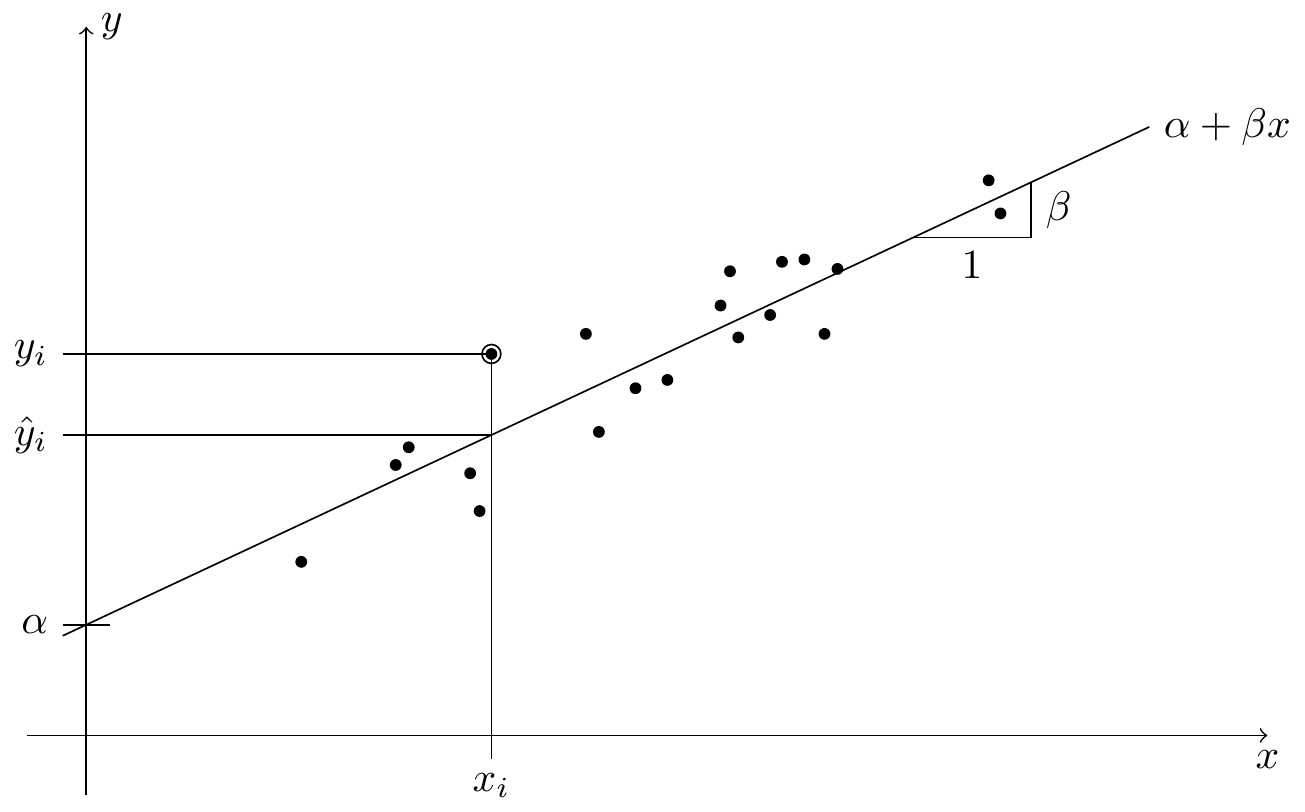
\includegraphics{MATH3714_files/figure-latex/scatter-plot-1} 

}

\caption{An illustration of linear regression. Each of the black circles in the plot stands for one paired sample \((x_i, y_i)\). The regression line \(x \mapsto \alpha + \beta x\), with intercept~\(\alpha\) and slope~\(\beta\), aims to predict the value of~\(y\) using the observed value~\(x\). For the marked sample \((x_i, y_i)\), the predicted \(y\)-value is \(\hat y\).}\label{fig:scatter-plot}
\end{figure}

In this situation, the variable \(x\) is called a \textbf{input}, feature, or
sometimes the explanatory variable or the ``independent variable''.
The variable \(y\) is called \textbf{response} or output, or sometimes the
``dependent variable'', and \(\varepsilon\) is called the \textbf{residual} or error.

Extending the situation of simple linear regression, in this module
we will consider multiple linear regression, where the response~\(y\)
is allowed to depend on several input variables. The corresponding
model is now
\begin{equation*}
  y_i = \alpha + \beta_1 x_{i1} + \cdots + \beta_p x_{ip} + \varepsilon_i
\end{equation*}
for all \(i \in \{1, 2, \ldots, p\}\), where \(n\) is still the number
of observations, and \(p\) is now the number of inputs we observe for
each sample.

Note that for multiple linear regression, we still consider a
single response for each sample, only the number of inputs has been
increased. One way to deal with situations where there is more than
one output would be to fit separate models for each output.

We will discuss multiple linear regression in much detail; our discussion
will be guided by three different aims of linear regression:

\begin{enumerate}
\def\labelenumi{\arabic{enumi}.}
\tightlist
\item
  Prediction: given a not previously observed value \(x\), try to predict
  the corresponding~\(y\).
\item
  In cases were the residuals \(\varepsilon_i\) correspond to unwanted noise,
  the fitted values \(\hat y_i = \alpha + \beta x_i\) can be considered
  to be de-noised versions of the observed values \(y_i\).
\item
  By studying a fitted regression model, sometimes better understanding
  of the data can be achieved. For example, one could ask whether
  all of the \(p\) input variables carry information about the response~\(y\).
\end{enumerate}

We will address these aims by considering different questions, like
how to estimate the coefficients \(\alpha, \beta_1, \ldots, \beta_p\),
how to assess model fit, or how to deal with outliers in the data.

\clearpage

\hypertarget{S00-about}{%
\section*{About MATH3714}\label{S00-about}}
\addcontentsline{toc}{section}{About MATH3714}

This module is \textbf{MATH3714 Linear Regression and Robustness}. The
module manager and lecturer is Dr Jochen Voss, and my email address is
\href{mailto:J.Voss@leeds.ac.uk}{\nolinkurl{J.Voss@leeds.ac.uk}}.

\hypertarget{notes}{%
\subsection*{Notes and videos}\label{notes}}
\addcontentsline{toc}{subsection}{Notes and videos}

The main way I expect you to learn the material for this course is by
reading these notes and by watching the accompanying videos. I will
release two sections of notes each week, for a total of 22 sections.

Reading mathematics is a slow process. Each section roughly
corresponds to one traditional lecture, which would have taken 50
minutes. If you find yourself regularly getting through sections in
much less than an hour, you're probably not reading carefully enough
through each sentence of explanation and each line of mathematics,
including understanding the motivation as well as checking the
accuracy.

It is possible (but not recommended) to learn the material by only
reading the notes and not watching the videos. It is not possible to
learn the material by only watching the videos and not reading the
notes.

Since we will all be relying heavily on these notes, I'm even more
keen than usual to hear about errors mathematical, typographical or
otherwise. Please, please \href{mailto:J.Voss@leeds.ac.uk}{email me} if
think you may have found any.

\hypertarget{lectures}{%
\subsection*{Lectures}\label{lectures}}
\addcontentsline{toc}{subsection}{Lectures}

There will be one online synchronous ``lecture'' session each week, on
Mondays at 2-3pm, with me, run through Microsoft Teams. These will
not be ``lectures'' in the traditional sense of the term, but will be an
opportunity to re-emphasise material you have already learned from
notes and videos, to give extra examples, and to answer common student
questions, with some degree of interactivity.

I will assume you have completed all the work for the previous week by
the time of the lecture, but I will not assume you've started the work
for that week itself.

I am very keen to hear about things you'd like to go through in the
lectures; please \href{mailto:J.Voss@leeds.ac.uk}{email me} with your
suggestions.

\hypertarget{workshops}{%
\subsection*{Workshops and Problem Sheets}\label{workshops}}
\addcontentsline{toc}{subsection}{Workshops and Problem Sheets}

There will be 5 problem sheets, corresponding to workshops in weeks 2,
4, 6, 8 and~10. The main goal of the workshops will be to go over
your answers to the problems sheets.

My recommended approach to problem sheets and workshops is the following:

\begin{itemize}
\tightlist
\item
  Work through the problem sheet before the workshop, spending plenty
  of time on it, and making multiple efforts at questions you get
  stuck on. I recommend spending \emph{at least three hours} on each
  problem sheet, in more than one block. Collaboration is encouraged
  when working through the problems, but I recommend writing up your
  work on your own.
\item
  Take advantage of the workshops to ask for help or clarification on
  questions you weren't able to complete.
\item
  After the workshop, attempt again the questions you were previously stuck on.
\item
  If you're still unable to complete a question after this second
  round of attempts, \emph{then} consult the solutions.
\end{itemize}

\hypertarget{teams}{%
\subsection*{Discussion Board}\label{teams}}
\addcontentsline{toc}{subsection}{Discussion Board}

I have set up \href{https://teams.microsoft.com/l/team/19\%3aopeKURHGjduA41CDtQUkmDjoPalh-zWDGuKhTk9zYq41\%40thread.tacv2/conversations?groupId=bde4675f-2c0d-4efd-9762-748cca83f4c4\&tenantId=bdeaeda8-c81d-45ce-863e-5232a535b7cb}{a Microsoft
Team}
for the course. I propose to use the ``Discussion'' channel there as a
discussion board. This is a good place to post questions about
material from the course, and --- even better! --- to help answer your
colleagues' questions. The idea is that you all as a group should help
each other out. I will visit a couple of times a week to clarify if
everybody is stumped by a question, or if there is disagreement.

\hypertarget{software}{%
\subsection*{Software}\label{software}}
\addcontentsline{toc}{subsection}{Software}

For the module we will use the statistical computing package R. This
program is free software, and you can find the program and
documentation at the \href{https://www.r-project.org/}{R project homepage}.
In particular, R will be used in the (assessed) practial.

My recommendation would be to install the \href{https://www.rstudio.com/}{RStudio
environment}, which includes R, on your own
computer and use this for your work. (Choose the open source
version, ``RStudio Desktop'', on the download page.) Alternatively you
can use RStudio or plain R on the university computers.

\hypertarget{assessments}{%
\subsection*{Assessments}\label{assessments}}
\addcontentsline{toc}{subsection}{Assessments}

Your final mark for the module will be based on a computer practical
(20\%) and a final exam (80\%). For the practical (I believe it will
take place in week 10) you will need to solve some problem using R and
the methods you learned in the course and to present your results in a
short report.

\clearpage

\hypertarget{S01-simple}{%
\section{Simple Linear Regression}\label{S01-simple}}

As a reminder, we consider simple linear regression in this section.
My hope is, that all of you have seen this material before at some
stage, \emph{e.g.}~in school or in some first or second year modules.

In preparation for notation introduced in the next section, we rename
the parameters from \(\alpha\) and \(\beta\) to the new names \(\beta_0\)
for the intercept and \(\beta_1\) for the slope.

\hypertarget{residual-sum-of-squares}{%
\subsection{Residual Sum of Squares}\label{residual-sum-of-squares}}

In simple linear regression, the aim is to find a regression line \(y = \beta_0 + \beta_1 x\), such that the line is ``close'' to given data points
\((x_1, y_1), \ldots, (x_n, y_n) \in\mathbb{R}^2\) for \(i \in \{1, 2, \ldots, n\}\). The ususal way to find \(alpha\) and \(\beta_1\), and thus the regression
line, is by minimising the \textbf{residual sum of squares}:
\begin{equation}
  r(\beta_0, \beta_1)
  = \sum_{i=1}^n \bigl( y_i - (\beta_0 + \beta_1 x_i) \bigr)^2.
  \label{eq:RSS}
\end{equation}
For given \(\beta_0\) and \(\beta_1\), the value \(r(\beta_0, \beta_1)\) measures
how close (in vertical direction) the given data points \((x_i, y_i)\)
are to the regression line \(\beta_0 + \beta_1 x\). By minimising
\(r(\beta_0, \beta_1)\) we find the regression line which is ``closest'' to
the data. The solution of this minimisation problem is usually
expressed in terms of the sample variance \(\mathrm{s}_x\) and the
sample covariance~\(\mathrm{s}_{xy}\).

\begin{definition}
\protect\hypertarget{def:sx}{}\label{def:sx}The \textbf{sample covariance} of \(x_1, \ldots, x_n \in \mathbb{R}\) and
\(y_1, \ldots, y_n\in\mathbb{R}\) is given by
\begin{equation*}
    \mathrm{s}_{xy}
    := \frac{1}{n-1} \sum_{i=1}^n (x_i - \bar x) (y_i - \bar y),
  \end{equation*}
where \(\bar x\) and \(\bar y\) are the sample means.

The \textbf{sample variance} of \(x_1, \ldots, x_n \in \mathbb{R}\) is given by
\begin{equation*}
    \mathrm{s}_{x}^2
    := \mathrm{s}_{xx}
    = \frac{1}{n-1} \sum_{i=1}^n (x_i - \bar x)^2,
  \end{equation*}
where, again, \(\bar x\) is the sample mean of the \(x_i\).
\end{definition}

\begin{lemma}
\protect\hypertarget{lem:simple-LSQ}{}\label{lem:simple-LSQ}Assume that \(\mathrm{s}_x^2 > 0\). Then the function \(r(\beta_0, \beta_1)\)
from~\eqref{eq:RSS} takes its minimum at the point \((\beta_0, \beta_1)\)
given by
\begin{equation*}
    \hat\beta_1 = \frac{\mathrm{s}_{xy}}{\mathrm{s}_x^2},
    \qquad
    \hat\beta_0 = \bar y - \hat \beta_1 \bar x,
  \end{equation*}
where \(\bar x, \bar y\) are the sample means, \(\mathrm{s}_{xy}\) is the
sample covariance and \(\mathrm{s}_x^2\) is the sample variance.
\end{lemma}

\begin{proof}
We could find the minimum of \(r\) by differentiating and setting the
derivatives to zero. Here we follow a different approach which uses
a ``trick'' to simplify the algebra: Let \(\tilde x_i = x_i - \bar x\)
and \(\tilde y_i = y_i - \bar y\) for all \(i \in \{1, \ldots, n\}\).
Then we have
\begin{equation*}
    \sum_{i=1}^n \tilde x_i
    = \sum_{i=1}^n x_i - n \bar x
    = 0
  \end{equation*}
and, similarly, \(\sum_{i=1}^n \tilde y_i = 0\). Using the new
coordinates \(\tilde x_i\) and \(\tilde y_i\) we find
\begin{align*}
    r(\beta_0, \beta_1)
    &= \sum_{i=1}^n \bigl(y_i - \beta_0 - \beta_1 x_i \bigr)^2 \\
    &= \sum_{i=1}^n \bigl( \tilde y_i + \bar y - \beta_0 - \beta_1 \tilde x_i - \beta_1 \bar x \bigr)^2 \\
    &= \sum_{i=1}^n \Bigl( \bigl( \tilde y_i - \beta_1 \tilde x_i \bigr)
    + \bigl( \bar y - \beta_0 - \beta_1 \bar x \bigr) \Bigr)^2 \\
    &= \sum_{i=1}^n \bigl( \tilde y_i - \beta_1 \tilde x_i \bigr)^2
    + 2 \bigl( \bar y - \beta_0 - \beta_1 \bar x \bigr) \sum_{i=1}^n \bigl( \tilde y_i - \beta_1 \tilde x_i \bigr)
    + n \bigl( \bar y - \beta_0 - \beta_1 \bar x \bigr)^2
  \end{align*}
Since \(\sum_{i=1}^n \tilde x_i = \sum_{i=1}^n \tilde y_i = 0\), the
second term on the right-hand side vanishes and we get
\begin{equation}
    r(\beta_0, \beta_1)
    = \sum_{i=1}^n \bigl( \tilde y_i - \beta_1 \tilde x_i \bigr)^2
    + n \bigl( \bar y - \beta_0 - \beta_1 \bar x \bigr)^2.  \label{eq:RSS-rewrite}
  \end{equation}
Both of these terms are positive and we can minimise the second term
(without changing the first term) by setting
\(\beta_0 = \bar y - \beta_1 \bar x\).

To find the value of \(\beta_1\) which minimises the first term on the
right-hand side of~\eqref{eq:RSS-rewrite} we now set the
(one-dimensional) derivative w.r.t.~\(\beta_1\) equal to~\(0\). We get
the condition
\begin{align*}
    0
    &\overset{!}{=} \frac{d}{d\beta_1} \sum_{i=1}^n \bigl( \tilde y_i - \beta_1 \tilde x_i \bigr)^2 \\
    &= \sum_{i=1}^n 2 \bigl( \tilde y_i - \beta_1 \tilde x_i \bigr) \frac{d}{d\beta_1} \bigl( \tilde y_i - \beta_1 \tilde x_i \bigr) \\
    &= - 2 \sum_{i=1}^n \bigl( \tilde y_i - \beta_1 \tilde x_i \bigr) \tilde x_i \\
    &= -2  \sum_{i=1}^n \tilde x_i \tilde y_i + 2 \beta_1 \sum_{i=1}^n \tilde x_i^2.
  \end{align*}
The only solution to this equation is
\begin{align*}
    \beta_1
    &= \frac{\sum_{i=1}^n \tilde x_i \tilde y_i}{\sum_{i=1}^n \tilde x_i^2} \\
    &= \frac{\sum_{i=1}^n (x_i - \bar x) (y_i - \bar y)}{\sum_{i=1}^n (x_i - \bar x)^2} \\
    &= \frac{\frac{1}{n-1}\sum_{i=1}^n (x_i - \bar x) (y_i - \bar y)}{\frac{1}{n-1}\sum_{i=1}^n (x_i - \bar x)^2} \\
    &= \frac{\mathrm{s}_{xy}}{\mathrm{s}_x^2}.
  \end{align*}
Since the second derivative is \(2 \sum_{i=1}^n \tilde x_i^2 \geq 0\),
this is indeed a minimum and the proof is complete.
\end{proof}

\hypertarget{linear-regression-as-a-parameter-estimation-problem}{%
\subsection{Linear Regression as a Parameter Estimation Problem}\label{linear-regression-as-a-parameter-estimation-problem}}

In statistics, any analysis starts by making a statistical model of
the data. This is done by writing random variables which have the
same structure as the data, and which are chosen so that the data
``looks like'' a random sample from these random variables.

To construct a model for the data used in a simple linear regression
problem, we use random variables \(Y_1, \ldots, Y_n\) such that
\begin{equation}
  Y_i
  = \beta_0 + \beta_1 x_i + \varepsilon_i \label{eq:regression}
\end{equation}
for all \(i \in \{1, 2, \ldots, n\}\), where \(\varepsilon_1, \ldots, \varepsilon_n\)
are i.i.d.~random variables with \(\mathbb{E}(\varepsilon_i) = 0\) and
\(\mathop{\mathrm{Var}}(\varepsilon_i) = \sigma^2\).

\begin{itemize}
\tightlist
\item
  Here we assume that the \(x\)-values are fixed and known. The only
  random quantities in the model are \(\varepsilon_i\) and~\(Y_i\). (There are
  more complicated models which also allow for randomness of \(x\), but
  we won't consider such models here.)
\item
  The random variables \(\varepsilon_i\) are called \textbf{residuals} or
  \textbf{errors}. In a scatter plot, the residuals correspond to the
  vertical distance between the samples and the regression line.
  Often one assumes that \(\varepsilon_i \sim \mathcal{N}(0, \sigma^2)\) for all
  \(i \in \{1, 2, \ldots, n\}\).
\item
  The values \(\beta_0\), \(\beta_1\) and \(\sigma^2\) are parameters of
  the model. To fit the model to data, we need to estimate these
  parameters.
\end{itemize}

This model is more complex than the models considered in some
introductory courses to statistics:

\begin{itemize}
\tightlist
\item
  The data consists now of pairs of numbers, instead of just
  single numbers.
\item
  We have
  \begin{equation*}
    \mathbb{E}(Y_i)
    = \mathbb{E}\bigl( \beta_0 + \beta_1 x_i + \varepsilon_i \bigr)
    = \beta_0 + \beta_1 x_i + \mathbb{E}(\varepsilon_i)
    = \beta_0 + \beta_1 x_i.
  \end{equation*}
  Thus, the expectation of \(Y_i\) depends on \(x_i\) and, at least for
  \(\beta_1 \neq 0\), the random variables \(Y_i\) are not identically
  distributed.
\end{itemize}

In this setup, we can consider the estimates \(\hat\beta_0\) and \(\hat\beta_1\)
from the previous subsection as statistcal parameter estimates for the
model parameters \(\beta_0\) and~\(\beta_1\).

In order to fit a linear model we also need to estimate the residual
variance~\(\sigma^2\). This can be done using the estimator
\begin{equation}
  \hat\sigma^2
  = \frac{1}{n-2} \sum_{i=1}^n \hat\varepsilon_i^2
  = \frac{1}{n-2} \sum_{i=1}^n (y_i - \hat\beta_0 - \hat\beta_1 x_i)^2.
  \label{eq:reg-sigma-est}
\end{equation}
To understand the form of this estimator, we have to remember that
\(\sigma^2\) is the variance of the \(\varepsilon_i\). Thus, using the standard
estimator for the variance, we could estimate \(\sigma^2\) as
\begin{equation}
  \sigma^2
  \approx \frac{1}{n-1} \sum_{i=1}^n \bigl(\varepsilon_i - \bar\varepsilon\bigr)^2
  \approx \frac{1}{n-1} \sum_{i=1}^n \bigl(\hat\varepsilon_i - \overline{\hat\varepsilon}\bigr)^2,
  \label{eq:resid-var-est}
\end{equation}

where \(\bar\varepsilon\) and \(\overline{\hat\varepsilon}\) are the averages of the
\(\varepsilon_i\) and the \(\hat\varepsilon_i\), respectively. One can show that
\(\overline{\hat\varepsilon} = 0\). The estimates of \(\beta_0\) and \(\beta_1\) are
sensitive to fluctuations in the data, with the effect that the
estimated regression line is, on average, slightly closer to the data
points than the true regression line would be. This causes the sample
variance of the \(\hat\varepsilon_i\), on average, to be slightly smaller than
the true residual variance \(\sigma^2\) and the thus the
estimator~\eqref{eq:resid-var-est} is slightly biased. A more
detailed analysis reveals that an unbiased estimator can be obtained
if one replaces the pre-factor \(1/(n-1)\) in equation~\eqref{eq:resid-var-est}
with \(1/(n-2)\). This leads to the estimator~\eqref{eq:reg-sigma-est}.

The main advantage gained by considering a statistical model is, that
we now can consider how close the estimators \(\hat\beta_0\), \(\hat\beta_1\)
and \(\hat\sigma^2\) are to the true values. Results one can obtain
include the following:

\begin{itemize}
\item
  The estimators \(\hat\beta_0\), \(\hat\beta_1\) and \(\hat\sigma^2\)
  are unbiased: This means that when we plug in random data
  \((x_i, Y_i)\) from the model~\eqref{eq:regression}, on
  average we get the correc answer: \(\mathbb{E}(\hat\beta_0) = \beta_0\),
  \(\mathbb{E}(\hat\beta_1) = \beta_1\), \(\mathbb{E}(\hat\sigma^2) = \sigma^2\).
\item
  One can ask about the average distance between the estimated
  parameters \(\hat\beta_0\), \(\hat\beta_1\) and \(\hat\sigma^2\)
  and the (unknown) true values \(\beta_0\), \(\beta_1\) and \(\sigma^2\).
  One measure for these distances is the root mean squared error
  of the estimators.
\item
  One can consider confidence intervals for the parameters
  \(\beta_0\), \(\beta_1\) and \(\sigma^2\).
\item
  One can consider statistical hypothesis tests to answer
  yes/no questions about the parameters. For example, one might ask
  whether the data could have come from the model with \(\beta_0=0\).
\item
  One can consider whether the data is compatible with the model
  at all, irrespective of parameter values. If there is a non-linear
  relationship between \(x\) and \(y\), the model~\eqref{eq:regression}
  will no longer be appropriate.
\end{itemize}

We will consider most of these questions over the course of the
module.

\hypertarget{sec:simple-mat}{%
\subsection{Matrix Notation}\label{sec:simple-mat}}

To conclude this section, we will rewrite the results of this section
in a form which we will extensively use for multiple linear regression
in the rest of this module. The idea here is to arrange all quantities
in the problem as matrices and vectors in order to simplify notation.
We write
\begin{equation*}
  X = \begin{pmatrix}
    1 & x_1\\ 1 & x_2\\\vdots & \vdots\\1 & x_n
  \end{pmatrix}
  \in \mathbb{R}^{n\times 2},
  \qquad
  y = \begin{pmatrix}
    y_1 \\ y_2 \\ \vdots \\ y_n
  \end{pmatrix}
  \in \mathbb{R}^n,
  \qquad
  \varepsilon= \begin{pmatrix}
    \varepsilon_1 \\ \varepsilon_2 \\ \vdots \\ \varepsilon_n
  \end{pmatrix}
  \in \mathbb{R}^n,
  \qquad
  \beta = \begin{pmatrix}
    \beta_0 \\
    \beta_1
  \end{pmatrix}
  \in\mathbb{R}^2
\end{equation*}
Using this notation, we can rewrite the \(n\) equations \(y_i = \beta_0 + x_i \beta_1 + \varepsilon_i\) for \(i \in \{1, \ldots, n\}\) as one
vector-valued equation in~\(\mathbb{R}^n\): we get
\begin{equation*}
  y = X\beta + \varepsilon,
\end{equation*}
and we want to ``solve'' this vector-valued equation for~\(\beta\).
The sum of squares can now be written as
\begin{equation*}
  r(\beta)
  = \sum_{i=1}^n \varepsilon_i^2
  = \varepsilon^\top \varepsilon
  = (y - X\beta)^\top (y - X\beta)
  = y^\top y - 2\beta^\top X^\top y + \beta^\top X^\top X \beta.
\end{equation*}
In the next section we will see that the minimum of \(r\) is attained
for
\begin{equation*}
  \hat\beta
  = (X X^\top)^{-1} X^\top y
\end{equation*}
and one can check that the components of this vector \(\hat\beta = (\hat\beta_0, \hat\beta_1)\) coincide with the estimates we obtained above.

\textbf{Summary}

\begin{itemize}
\tightlist
\item
  simple linear regression is the case where there is only one input
\item
  a regression line is fitted by minimising the residual sum of squares
\item
  linear regression is a statistical parameter estimation problem
\item
  the problem can be conveniently written in matrix/vector notation
\end{itemize}

\clearpage

\hypertarget{S02-multiple}{%
\section{Least Squares Estimates}\label{S02-multiple}}

\hypertarget{data-and-models}{%
\subsection{Data and Models}\label{data-and-models}}

For multiple linear regression we assume that there are \(p\) inputs and
one output. If we have a sample of \(n\) obervations, we have \(np\)
inputs and one output in total. Here we denote the \(i\)th observation
of the \(j\)th input by \(x_{ij}\) and the corresponding output by~\(y_j\).

As an example, we consider the \texttt{mtcars} dataset built into R. This is
a small dataset, which contains information about 32 automobiles
(1973--74 models). The table lists fuel consumption \texttt{mpg}, gross horsepower \texttt{hp},
and 9 other aspects of these cars. Here we consider \texttt{mpg} to be the output,
and the other listed aspects to be inputs. Type \texttt{help(mtcars)} in R to learn
more about this dataset:

\begin{Shaded}
\begin{Highlighting}[]
\NormalTok{mtcars}
\end{Highlighting}
\end{Shaded}

\begin{Shaded}
\begin{Highlighting}[]
\NormalTok{\#                      mpg cyl  disp  hp drat    wt  qsec vs am gear carb}
\NormalTok{\# Mazda RX4           21.0   6 160.0 110 3.90 2.620 16.46  0  1    4    4}
\NormalTok{\# Mazda RX4 Wag       21.0   6 160.0 110 3.90 2.875 17.02  0  1    4    4}
\NormalTok{\# Datsun 710          22.8   4 108.0  93 3.85 2.320 18.61  1  1    4    1}
\NormalTok{\# Hornet 4 Drive      21.4   6 258.0 110 3.08 3.215 19.44  1  0    3    1}
\NormalTok{\# Hornet Sportabout   18.7   8 360.0 175 3.15 3.440 17.02  0  0    3    2}
\NormalTok{\# Valiant             18.1   6 225.0 105 2.76 3.460 20.22  1  0    3    1}
\NormalTok{\# Duster 360          14.3   8 360.0 245 3.21 3.570 15.84  0  0    3    4}
\NormalTok{\# Merc 240D           24.4   4 146.7  62 3.69 3.190 20.00  1  0    4    2}
\NormalTok{\# Merc 230            22.8   4 140.8  95 3.92 3.150 22.90  1  0    4    2}
\NormalTok{\# Merc 280            19.2   6 167.6 123 3.92 3.440 18.30  1  0    4    4}
\NormalTok{\# Merc 280C           17.8   6 167.6 123 3.92 3.440 18.90  1  0    4    4}
\NormalTok{\# Merc 450SE          16.4   8 275.8 180 3.07 4.070 17.40  0  0    3    3}
\NormalTok{\# Merc 450SL          17.3   8 275.8 180 3.07 3.730 17.60  0  0    3    3}
\NormalTok{\# Merc 450SLC         15.2   8 275.8 180 3.07 3.780 18.00  0  0    3    3}
\NormalTok{\# Cadillac Fleetwood  10.4   8 472.0 205 2.93 5.250 17.98  0  0    3    4}
\NormalTok{\# Lincoln Continental 10.4   8 460.0 215 3.00 5.424 17.82  0  0    3    4}
\NormalTok{\# Chrysler Imperial   14.7   8 440.0 230 3.23 5.345 17.42  0  0    3    4}
\NormalTok{\# Fiat 128            32.4   4  78.7  66 4.08 2.200 19.47  1  1    4    1}
\NormalTok{\# Honda Civic         30.4   4  75.7  52 4.93 1.615 18.52  1  1    4    2}
\NormalTok{\# Toyota Corolla      33.9   4  71.1  65 4.22 1.835 19.90  1  1    4    1}
\NormalTok{\# Toyota Corona       21.5   4 120.1  97 3.70 2.465 20.01  1  0    3    1}
\NormalTok{\# Dodge Challenger    15.5   8 318.0 150 2.76 3.520 16.87  0  0    3    2}
\NormalTok{\# AMC Javelin         15.2   8 304.0 150 3.15 3.435 17.30  0  0    3    2}
\NormalTok{\# Camaro Z28          13.3   8 350.0 245 3.73 3.840 15.41  0  0    3    4}
\NormalTok{\# Pontiac Firebird    19.2   8 400.0 175 3.08 3.845 17.05  0  0    3    2}
\NormalTok{\# Fiat X1{-}9           27.3   4  79.0  66 4.08 1.935 18.90  1  1    4    1}
\NormalTok{\# Porsche 914{-}2       26.0   4 120.3  91 4.43 2.140 16.70  0  1    5    2}
\NormalTok{\# Lotus Europa        30.4   4  95.1 113 3.77 1.513 16.90  1  1    5    2}
\NormalTok{\# Ford Pantera L      15.8   8 351.0 264 4.22 3.170 14.50  0  1    5    4}
\NormalTok{\# Ferrari Dino        19.7   6 145.0 175 3.62 2.770 15.50  0  1    5    6}
\NormalTok{\# Maserati Bora       15.0   8 301.0 335 3.54 3.570 14.60  0  1    5    8}
\NormalTok{\# Volvo 142E          21.4   4 121.0 109 4.11 2.780 18.60  1  1    4    2}
\end{Highlighting}
\end{Shaded}

For this dataset we have \(n = 32\) (number of cars), and \(p = 10\) (number
of attributes, excluding \texttt{mpg}). The values \(y_1, \ldots, y_{32}\) are listed
in the first column of the table, the values \(x_{i,1}\) for \(i \in \{1, \ldots, 32\}\) are shown in the second column, and the values \(x_{i,10}\) are shown in
the last column.

In this dataset it is easy to make scatter plots which show how a single
input affects the output. For example, we can show how the engine power
affects fuel consumption:

\begin{Shaded}
\begin{Highlighting}[]
\FunctionTok{plot}\NormalTok{(mtcars}\SpecialCharTok{$}\NormalTok{hp, mtcars}\SpecialCharTok{$}\NormalTok{mpg,}
     \AttributeTok{xlab =} \StringTok{"power [hp]"}\NormalTok{, }\AttributeTok{ylab =} \StringTok{"fuel consumption [mpg]"}\NormalTok{)}
\end{Highlighting}
\end{Shaded}

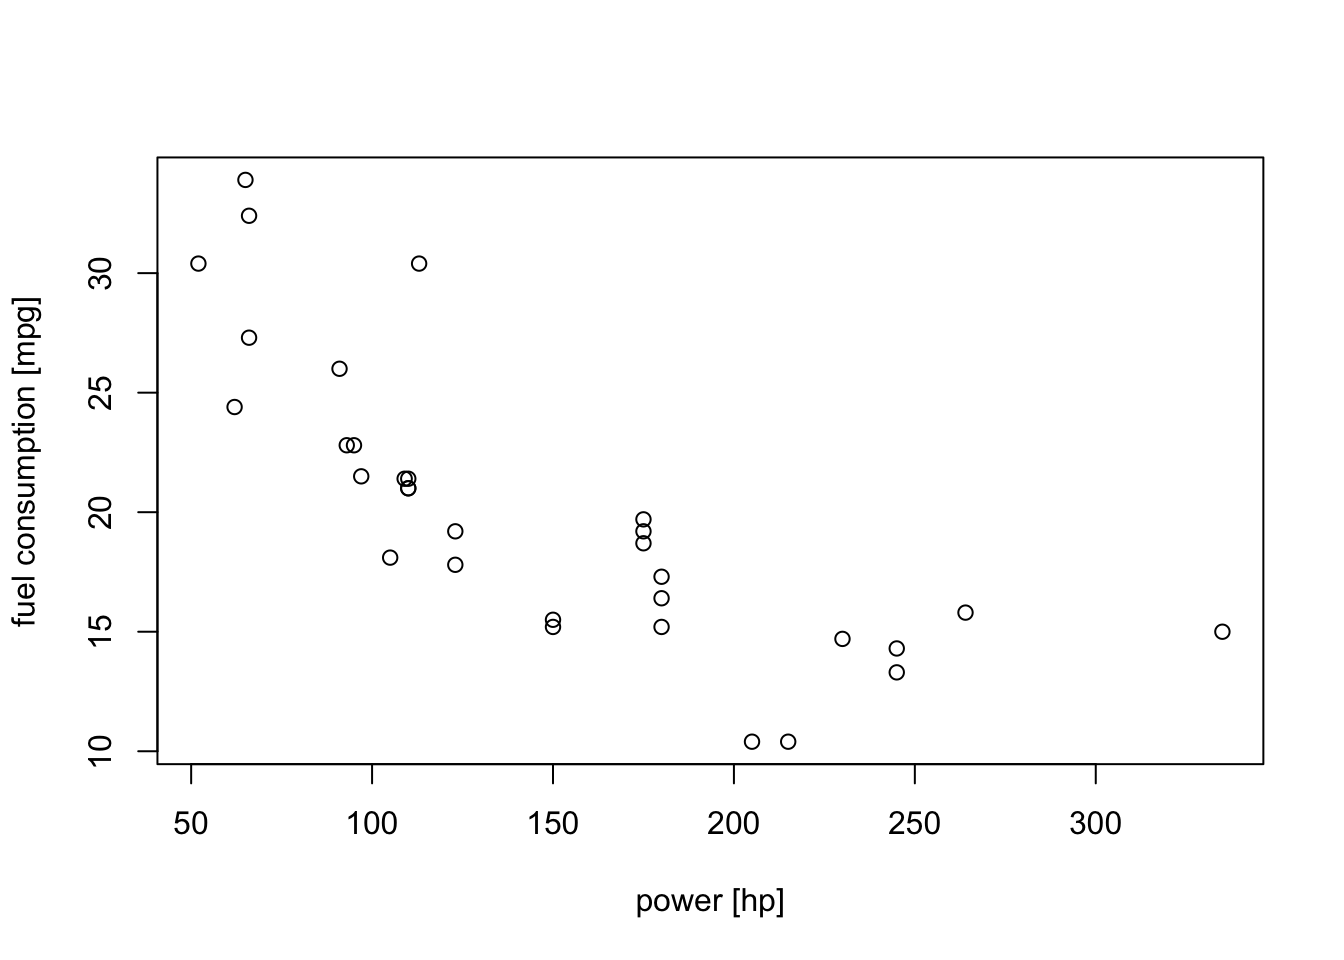
\includegraphics{MATH3714_files/figure-latex/mtcars-hp-mpg-plot-1.pdf}

We can see that cars with stronger engines tend to use more fuel
(\emph{i.e.}~a gallon of fuel lasts for fewer miles; the curve goes down),
but leaving out the other inputs omits a lot of information. It is
not easy to make a plot which takes all inputs into account. Is is
also not immediately obvious which of the variables are most
important.

In linear regression, we assume that the output depends on the
inputs in a linear (or more precisely, \emph{affine}) way. We write
this as
\begin{equation}
  y_i
  = \beta_0 + \beta_1 x_{i,1} + \cdots + \beta_p x_{i,p} + \varepsilon_i \label{eq:lmdata}
\end{equation}
where the residuals~\(\varepsilon_i\) are assumed to be ``small''.

The parameters \(\beta_j\) can be interpreted as the expected change in
the response \(y\) per unit change in \(x_j\) when all other regressor
variables are held fixed. For this reason the parameters \(\beta_j\)
(for \(j=1, \ldots, p\)) are sometimes called \emph{partial} regression
coefficients.

This model describes a hyperplane in the \((p+1)\)-dimensional space of
the inputs \(x_j\) and the output~\(y\). The hyperplane is easily
visualized when \(p=1\) (as a line in~\(\mathbb{R}^2\)), and visualisation can be
attempted for \(p=2\) (as a plane in \(\mathbb{R}^3\)) but is very hard for \(p>2\).

We defer making a proper statistical model for multiple linear regression
until the next section.

\hypertarget{the-normal-equations}{%
\subsection{The Normal Equations}\label{the-normal-equations}}

Similar to what we did in Section~\ref{sec:simple-mat}, we rewrite
the model using matrix notation. We define the vectors
\begin{equation*}
  y = \begin{pmatrix}
    y_1 \\ y_2 \\ \vdots \\ y_n
  \end{pmatrix}
  \in \mathbb{R}^n,
  \qquad
  \varepsilon= \begin{pmatrix}
    \varepsilon_1 \\ \varepsilon_2 \\ \vdots \\ \varepsilon_n
  \end{pmatrix}
  \in \mathbb{R}^n,
  \qquad
  \beta = \begin{pmatrix}
    \beta_0 \\
    \beta_1 \\
    \vdots \\
    \beta_p
  \end{pmatrix}
  \in\mathbb{R}^{1+p}
\end{equation*}
as well as the matrix
\begin{equation*}
  X = \begin{pmatrix}
    1 & x_{1,1} & \cdots & x_{1,p} \\
    1 & x_{2,1} & \cdots & x_{2,p} \\
    \vdots & \vdots & & \vdots \\
    1 & x_{n,1} & \cdots & x_{n,p} \\
  \end{pmatrix}
  \in \mathbb{R}^{n\times (1+p)}.
\end{equation*}
The parameters \(\beta_i\) are called the \textbf{regression coefficients} and
the matrix \(X\) is called the \textbf{design matrix}.

Using this notation, the model~\eqref{eq:lmdata} can be written
as
\begin{equation}
  y = X \beta + \varepsilon,  \label{eq:lmmodel}
\end{equation}
where again \(X\beta\) is a matrix-vector multiplication which ``hides''
the sums in equation~\eqref{eq:lmdata}, and \eqref{eq:lmmodel}
is an equation of vectors of size~\(n\), which combines the \(n\)
individual equations from \eqref{eq:lmdata} for the different
values of~\(i\).

To simplify notation, we index the columns of \(X\) by \(0, 1, \ldots, p\) (instead of the more conventional \(1, \ldots, p+1\)), so that we
can for example write
\begin{equation*}
  (X \beta)_i
  = \sum_{j=0}^p x_{i,j} \beta_j
  = \beta_0 + \sum_{j=1}^p x_{i,j} \beta_j.
\end{equation*}

As before, we find the regression coefficients by minimising
the residual sum of squares:
\begin{align*}
  r(\beta)
  &= \sum_{i=1}^n \varepsilon_i^2 \\
  &= \sum_{i=1}^n \bigl( y_i - (\beta_0 + \beta_1 x_{i,1} + \cdots + \beta_p x_{i,p}) \bigr)^2.
\end{align*}
In practice, this notation turns out to be cumbersome, and we will
use matrix notation in the following proof.

\begin{lemma}
\protect\hypertarget{lem:multiple-LSQ}{}\label{lem:multiple-LSQ}Assume that the matrix \(X^\top X \in \mathbb{R}^{(1+p) \times (1+p)}\) is
invertible. Then the function \(r(\beta)\) takes its minimum at the
vector \(\hat\beta\in\mathbb{R}^{p+1}\) given by
\begin{equation*}
  \hat\beta
  = (X^\top X)^{-1} X^\top y.
\end{equation*}
\end{lemma}

\begin{proof}
Using the vector equation \(\varepsilon= y - X \beta\), we can also write the
residual sum of squares as
\begin{align*}
    r(\beta)
    &= \sum_{i=1}^n \varepsilon_i^2 \\
    &= \varepsilon^\top \varepsilon\\
    &= (y - X \beta)^\top (y - X \beta) \\
    &= y^\top y - y^\top X\beta - (X\beta)^\top y + (X\beta)^\top (X\beta).
  \end{align*}
Using the linear algebra rules from Appendix~\ref{matrix-rules} we find
that \(y^\top X\beta = (X\beta)^\top y = \beta^\top X^\top y\)
and \((X\beta)^\top (X\beta) = \beta^\top X^\top X \beta\). Thus we get
\begin{equation*}
    r(\beta)
    = y^\top y - 2\beta^\top X^\top y + \beta^\top X^\top X \beta.
  \end{equation*}
Note that in this equation \(X\) is a matrix, \(y\) and \(\beta\) are vectors,
and \(r(\beta)\) is a number.

To find the minimum of this function, we set all partial derivatives
\(\frac{\partial}{\partial \beta_i} r(\beta)\) equal to~\(0\). Going through the terms in
the formula for \(r(\beta)\) we find: (1) \(y^\top y\) does not depend on \(\beta\),
so we have \(\frac{\partial}{\partial \beta_i} y^\top y = 0\) for all \(i\), (2) we have
\begin{equation*}
    \frac{\partial}{\partial \beta_i} \beta^\top X^\top y
    = \frac{\partial}{\partial \beta_i} \sum_{j=1}^{p+1} \beta_j (X^\top y)_j
    = (X^\top y)_i
  \end{equation*}
and (3) finally
\begin{equation*}
    \frac{\partial}{\partial \beta_i} \beta^\top X^\top X \beta
    = \frac{\partial}{\partial \beta_i} \sum_{j,k=1}^{p+1} \beta_j (X^\top X)_{j,k} \beta_k
    = 2 \sum_{k=1}^{p+1} (X^\top X)_{i,k} \beta_k
    = 2 \bigl( (X^\top X) \beta \bigr)_i.
  \end{equation*}
(Some care is needed, when checking that the middle equality sign in
the previous equation is correct.)
Combining these derivatives, we find
\begin{equation}
    \frac{\partial}{\partial \beta_i} r(\beta)
    = 0 - 2 (X^\top y)_i + 2 \bigl( X^\top X \beta \bigr)_i
                           \label{eq:normal-first}
  \end{equation}
for all \(i \in \{0, 1, \ldots, p\}\). At a local minimum of \(r\),
all of these partial derivatives must be zero and using a vector
equation we find that a necessary condition for a minimum is
\begin{equation}
    X^\top X \beta = X^\top y.  \label{eq:normal-equations}
  \end{equation}
Since we assumed that \(X^\top X\) is invertible, there is exactly
one vector \(\beta\) which solves \eqref{eq:normal-equations}. This
vector is given by
\begin{equation*}
    \hat\beta
    := (X^\top X)^{-1} X^\top y.
  \end{equation*}

As for one-dimensional minimisation, there is a condition on the
second derivatives which must be checked to see which local extrema
are local minima. Here we are only going to sketch this argument: A
sufficient condition for \(\hat\beta\) to be a minimum is for the
second derivative matrix (\href{https://en.wikipedia.org/wiki/Hessian_matrix}{the Hessian
matrix})
to be positive definite (see appendix~\ref{positive-definite}).
Using equation~\eqref{eq:normal-first} we find
\begin{equation*}
    \frac{\partial}{\partial\beta_i \partial\beta_j} r(\beta)
    = 2 (X^\top X)_{i,j}
  \end{equation*}
And thus the Hessian matrix is \(H = 2 X^\top X\). Using results from
linear algebra, one can show that this matrix is indeed positive
definite and thus \(\hat\beta\) is the unique minimum of~\(r\).
\end{proof}

Equation~\eqref{eq:normal-equations} gives a system of \(p+1\) linear
equations with \(p+1\) unknowns. This system of linear equations,
\(X^\top X \beta = X^\top y\) is called the \textbf{normal equations}.
If \(X^\top X\) is invertible, as assumed in the lemma, this
system of equations has \(\hat\beta\) as its unique solution.
Otherwise, there may be more than one \(\beta\) which leads to the
same value \(r(\beta)\) and the minimum will no longer be unique.
This happens for example, if two of the inputs are identical to
each other (or, more generally, one input is linearly dependent
on one or more other inputs).

The condition that \(X^\top X\) must be invertible in multiple linear
regression corresponds to the condition \(\mathrm{s}_x^2 > 0\) from
lemma~\ref{lem:simple-LSQ} for simple linear regression.

The value \(\hat\beta\) found in the lemma is called the \textbf{least squares
estimator} for \(\beta\), or sometimes the ordinary least squares (OLS)
estimator.

\hypertarget{fitted-values}{%
\subsection{Fitted Values}\label{fitted-values}}

Let us again consider our model
\begin{equation*}
  y = X \beta + \varepsilon,
\end{equation*}
using the matrix notation introduced above. Here we can think of
\(X\beta\) as the \textbf{true values}, while \(\varepsilon\) are the errors. The
design matrix \(X\) (containing the inputs) and the response \(y\) are
known to us, while the true coefficients \(\beta\) and the errors \(\varepsilon\)
are unknown. Solving for \(\varepsilon\) we find that the errors satisfy
\begin{equation*}
  \varepsilon= y - X\beta.
\end{equation*}

Using the least squares estimate \(\hat\beta\) we can estimate the true
values as
\begin{equation}
  \hat y = X \hat\beta.  \label{eq:fitted-values}
\end{equation}
These estimates are called the \textbf{fitted values}. Using the
definition of \(\hat\beta\) we get
\begin{equation*}
  \hat y
  = X (X^\top X)^{-1} X^\top y
  =: Hy.
\end{equation*}
The matrix \(H = X (X^\top X)^{-1} X^\top\) is commonly called the \textbf{hat
matrix} (because it ``puts the hat on \(y\)'').

Finally, we can estimate the errors using the residuals
\begin{equation}
  \hat\varepsilon
  = y - X \hat\beta
  = y - \hat y
  = y - H y
  = (I - H) y,  \label{eq:fitted-errors}
\end{equation}
where \(I\) is the \((p+1)\times (p+1)\) identity matrix.

\hypertarget{example}{%
\subsection{Example}\label{example}}

To conclude this section, we demonstrate how these methods can be used
in R. For this we consider the \texttt{mtcars} example from the beginning of
the section again. I will first show how to do the analysis ``by hand'',
and later show how the same result can be obtained using R's built-in functions.

We first split \texttt{mtcars} into the respons column \texttt{y} (the first column)
and the design matrix \texttt{X} (a column of ones, followed by columns 2 to 11
of \texttt{mtcars}):

\begin{Shaded}
\begin{Highlighting}[]
\NormalTok{y }\OtherTok{\textless{}{-}}\NormalTok{ mtcars[, }\DecValTok{1}\NormalTok{]}
\NormalTok{X }\OtherTok{\textless{}{-}} \FunctionTok{cbind}\NormalTok{(}\DecValTok{1}\NormalTok{, }\FunctionTok{data.matrix}\NormalTok{(mtcars[, }\DecValTok{2}\SpecialCharTok{:}\DecValTok{11}\NormalTok{]))}
\end{Highlighting}
\end{Shaded}

Next we compute \(X^\top X\) and solve the normal equations. Often it is
faster, easier, and has lower numerical errors to solve the normal equations
rather than inverting the matrix \(X^\top X\).

\begin{Shaded}
\begin{Highlighting}[]
\NormalTok{XtX }\OtherTok{\textless{}{-}} \FunctionTok{t}\NormalTok{(X) }\SpecialCharTok{\%*\%}\NormalTok{ X}
\NormalTok{beta.hat }\OtherTok{\textless{}{-}} \FunctionTok{solve}\NormalTok{(XtX, }\FunctionTok{t}\NormalTok{(X) }\SpecialCharTok{\%*\%}\NormalTok{ y)}
\NormalTok{beta.hat}
\end{Highlighting}
\end{Shaded}

\begin{Shaded}
\begin{Highlighting}[]
\NormalTok{\#             [,1]}
\NormalTok{\#      12.30337416}
\NormalTok{\# cyl  {-}0.11144048}
\NormalTok{\# disp  0.01333524}
\NormalTok{\# hp   {-}0.02148212}
\NormalTok{\# drat  0.78711097}
\NormalTok{\# wt   {-}3.71530393}
\NormalTok{\# qsec  0.82104075}
\NormalTok{\# vs    0.31776281}
\NormalTok{\# am    2.52022689}
\NormalTok{\# gear  0.65541302}
\NormalTok{\# carb {-}0.19941925}
\end{Highlighting}
\end{Shaded}

Without further checks it is hard to know whether the result is correct, or
whether we made a mistake somewhere along the lines. One good sign is that
we argued earlier that higher \texttt{hp} should lead to lower \texttt{mpg}, and indeed the
corresponding coefficient \texttt{-0.02148212} is negative.

Finally, compute the fitted values and generate a plot of fitted values
against responses. If everything worked, we would expect the points in this
plot to be close to the diagonal.

\begin{Shaded}
\begin{Highlighting}[]
\NormalTok{y.hat }\OtherTok{\textless{}{-}}\NormalTok{ X }\SpecialCharTok{\%*\%}\NormalTok{ beta.hat}
\FunctionTok{plot}\NormalTok{(y, y.hat, }\AttributeTok{xlab =} \StringTok{"responses"}\NormalTok{, }\AttributeTok{ylab =} \StringTok{"fitted values"}\NormalTok{)}
\FunctionTok{abline}\NormalTok{(}\AttributeTok{a =} \DecValTok{0}\NormalTok{, }\AttributeTok{b =} \DecValTok{1}\NormalTok{) }\CommentTok{\# plot the diagonal}
\end{Highlighting}
\end{Shaded}

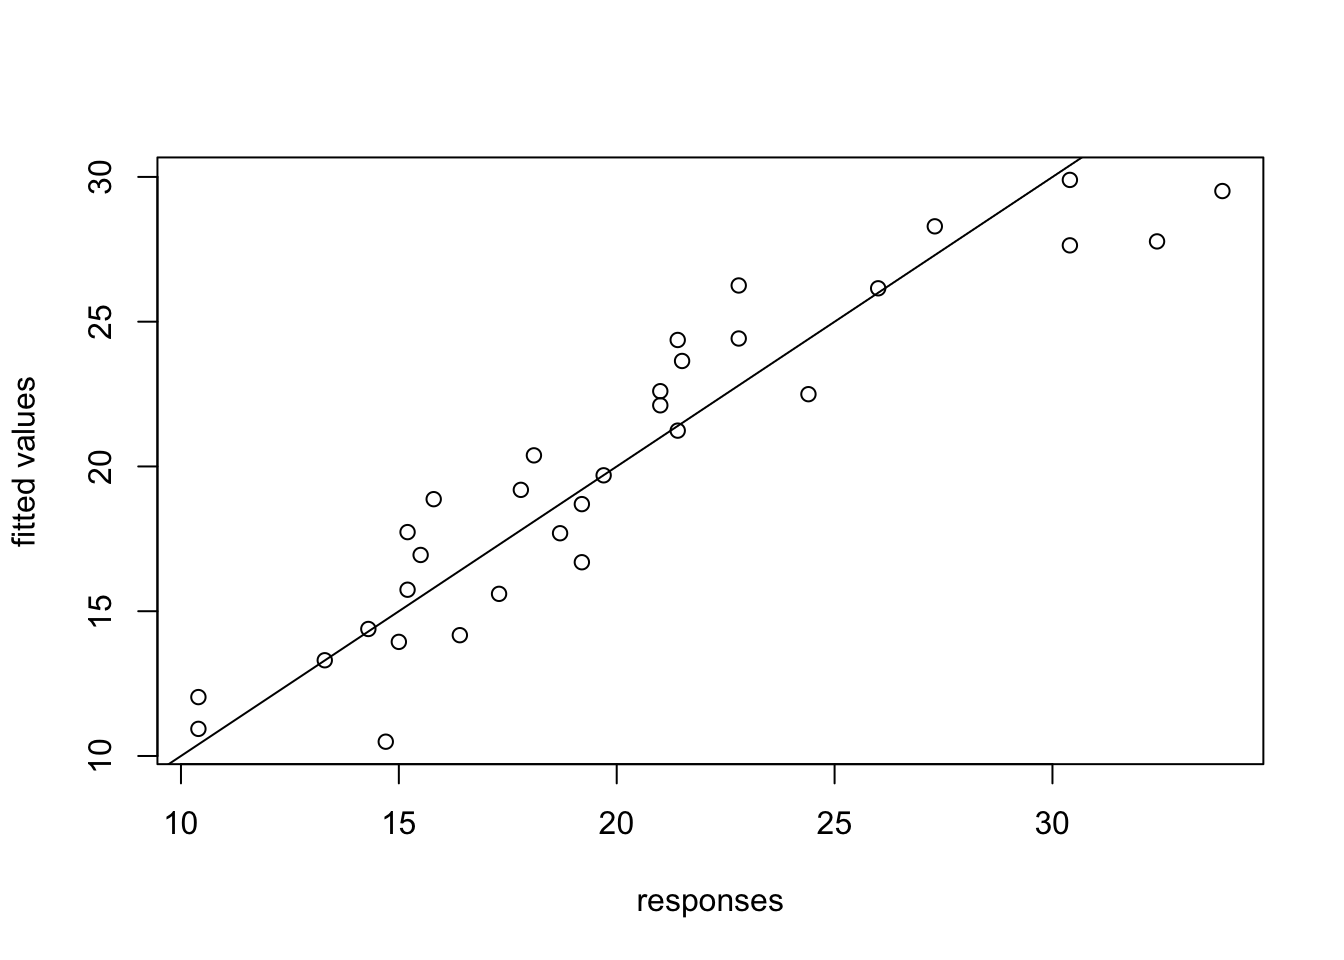
\includegraphics{MATH3714_files/figure-latex/y-y.hat-plot-1.pdf}

For comparison we now re-do the analysis using built-in R commands.
In the \texttt{lm()} command below, we use \texttt{data=mtcars} to tell R where the
data is stored, and the formula \texttt{mpg\ \textasciitilde{}\ .} states that we want to
model \texttt{mpg} as a function of all other variable (this is the meaning of \texttt{.}).

\begin{Shaded}
\begin{Highlighting}[]
\NormalTok{m }\OtherTok{\textless{}{-}} \FunctionTok{lm}\NormalTok{(mpg }\SpecialCharTok{\textasciitilde{}}\NormalTok{ ., }\AttributeTok{data =}\NormalTok{ mtcars) }\CommentTok{\# fit a linear model}
\FunctionTok{coef}\NormalTok{(m) }\CommentTok{\# get the estimated coefficients}
\end{Highlighting}
\end{Shaded}

\begin{Shaded}
\begin{Highlighting}[]
\NormalTok{\# (Intercept)         cyl        disp          hp        drat          wt }
\NormalTok{\# 12.30337416 {-}0.11144048  0.01333524 {-}0.02148212  0.78711097 {-}3.71530393 }
\NormalTok{\#        qsec          vs          am        gear        carb }
\NormalTok{\#  0.82104075  0.31776281  2.52022689  0.65541302 {-}0.19941925}
\end{Highlighting}
\end{Shaded}

Comparing these coefficients to the vector \texttt{beta.hat} from above shows
that we got the same result using both methods. The fitted values
can be computed using \texttt{fitted.values(m)}. Here we just check that we get
the same result as above:

\begin{Shaded}
\begin{Highlighting}[]
\FunctionTok{max}\NormalTok{(}\FunctionTok{abs}\NormalTok{(}\FunctionTok{fitted.values}\NormalTok{(m) }\SpecialCharTok{{-}}\NormalTok{ y.hat))}
\end{Highlighting}
\end{Shaded}

\begin{Shaded}
\begin{Highlighting}[]
\NormalTok{\# [1] 3.410605e{-}13}
\end{Highlighting}
\end{Shaded}

This results \texttt{5.329071e-13} stands for the number \(5.329071 \cdot 10^{-13}\),
which is extremely small. The difference between our results and R's result
is caused by rounding errors.

\textbf{Summary}

\begin{itemize}
\tightlist
\item
  multiple linear regression allows for more than one input
  but still has only one output
\item
  the least squared estimate for the coefficients is found
  by minimising the residual sum of squares
\item
  the estimate can be computed as the solution to the normal equations
\item
  the hat matrix transforms responses into fitted values
\end{itemize}

\clearpage

\hypertarget{I01-lm}{%
\section*{Interlude: Linear Regression in R}\label{I01-lm}}
\addcontentsline{toc}{section}{Interlude: Linear Regression in R}

\hypertarget{lm-fitting}{%
\subsection*{Fitting a Model}\label{lm-fitting}}
\addcontentsline{toc}{subsection}{Fitting a Model}

The function \texttt{lm()} is used to fit a linear model in~R. There are different
ways to specify the form of the model and the data to be used for fitting the
model.

\begin{itemize}
\item
  The most basic way to call \texttt{lm()} is the case where the explanatory
  variables and the response variable are stored as separate vectors.
  Assuming, for example, that the explanatory variables are \texttt{x1}, \texttt{x2}, \texttt{x3}
  and that the response variable is~\texttt{y} in~R, we can tell R to fit the
  linear model \(y = \beta_0 + \beta_1 x_1 + \beta_2 x_2 + \beta_3 x_3 + \varepsilon\)
  by using the following command:

\begin{Shaded}
\begin{Highlighting}[]
  \FunctionTok{lm}\NormalTok{(y }\SpecialCharTok{\textasciitilde{}}\NormalTok{ x1 }\SpecialCharTok{+}\NormalTok{ x2 }\SpecialCharTok{+}\NormalTok{ x3)}
\end{Highlighting}
\end{Shaded}

  Note that R automatically added the intercept term \(\beta_0\) to this
  model. If we want to fit a model without an intercept,
  \emph{i.e.} the model
  \(y = \beta_1 x_1 + \beta_2 x_2 + \beta_3 x_3 + \varepsilon\), we have to add
  \texttt{0\ +} in front of the explanatory variables:

\begin{Shaded}
\begin{Highlighting}[]
    \FunctionTok{lm}\NormalTok{(y }\SpecialCharTok{\textasciitilde{}} \DecValTok{0} \SpecialCharTok{+}\NormalTok{ x1 }\SpecialCharTok{+}\NormalTok{ x2 }\SpecialCharTok{+}\NormalTok{ x3)}
\end{Highlighting}
\end{Shaded}

  The general form of a model specification is the response variable,
  followed by \texttt{\textasciitilde{}}, followed by a plus-separated list of explanatory
  variables. For this form of calling \texttt{lm()}, the variables \texttt{y},
  \texttt{x1}, \texttt{x2}, and \texttt{x3} in the examples above must be already defined before
  \texttt{lm()} is called. It may be a good idea to double-check that the variables
  have the correct values before trying to call~\texttt{lm()}.
\item
  Both for the response and for explanatory variables we can
  specify arbitrary R expressions to compute the numeric values to be
  used. For example, to fit the model
  \(\log(y) = \beta_0 + \beta_1 x_1 + \beta_2 x_2 + \varepsilon\) (assuming
  that all \(y_i\) are positive) we can use the following command:

\begin{Shaded}
\begin{Highlighting}[]
  \FunctionTok{lm}\NormalTok{(}\FunctionTok{log}\NormalTok{(y) }\SpecialCharTok{\textasciitilde{}}\NormalTok{ x1 }\SpecialCharTok{+}\NormalTok{ x2)}
\end{Highlighting}
\end{Shaded}

  Some care is needed, because \texttt{+}, \texttt{*} and \texttt{\^{}} have a
  special meaning inside the first argument of \texttt{lm()}; any time
  we want to compute a variable for \texttt{lm()} using these
  operations, we need to surround the corresponding expression with
  \texttt{I()}, to tell R that \texttt{+}, \texttt{*} or \texttt{\^{}} should
  have their usual, arithmetic meaning. For example, to fit a model
  of the form \(y \sim \beta_0 + \beta_1 x + \beta_2 x^2 + \varepsilon\), we
  can use the following R command:

\begin{Shaded}
\begin{Highlighting}[]
  \FunctionTok{lm}\NormalTok{(y }\SpecialCharTok{\textasciitilde{}}\NormalTok{ x }\SpecialCharTok{+} \FunctionTok{I}\NormalTok{(x}\SpecialCharTok{\^{}}\DecValTok{2}\NormalTok{))}
\end{Highlighting}
\end{Shaded}

  Here, the use of \texttt{I()} tells R that \texttt{x\^{}2} is to be
  interpreted as the vector \((x_1^2, \ldots, x_n^2)\). Similarly, we
  can fit a model of the form
  \(y = \beta_0 + \beta_1 (x_1 + x_2) + \varepsilon\):

\begin{Shaded}
\begin{Highlighting}[]
  \FunctionTok{lm}\NormalTok{(y }\SpecialCharTok{\textasciitilde{}} \FunctionTok{I}\NormalTok{(x1}\SpecialCharTok{+}\NormalTok{x2))}
\end{Highlighting}
\end{Shaded}

  Here, the use of \texttt{I()} tells R that \texttt{x1+x2} indicates the
  vector \((x_{1,1}+x_{2,1}, \ldots, x_{1,n}+x_{2,n})\) instead of two
  separate explanatory variables.

  Details about how to specify models in calls to \texttt{lm()} can be found by
  using the \href{https://rdrr.io/r/stats/formula.html}{command \texttt{help(formula)}}
  in~R.
\item
  If the response and the explanatory variables are stored in the
  columns of a data frame, we can use the \texttt{data=...} argument to \texttt{lm()} to
  specify this data frame and then just use the column names to specify the
  regression model. For example, the
  \href{https://rdrr.io/r/datasets/stackloss.html}{\texttt{stackloss} dataset}
  built into R consists of a data frame with columns \texttt{Air.Flow},
  \texttt{Water.Temp}, \texttt{Acid.Conc.}, \texttt{stack.loss}. To predict
  \texttt{stackloss\$stack.loss} from \texttt{stackloss\$Air.Flow} we can write

\begin{Shaded}
\begin{Highlighting}[]
  \FunctionTok{lm}\NormalTok{(stack.loss }\SpecialCharTok{\textasciitilde{}}\NormalTok{ Air.Flow, }\AttributeTok{data=}\NormalTok{stackloss)}
\end{Highlighting}
\end{Shaded}

  As a special case, a single dot ``\texttt{.}'' can be used in place of
  the explanatory variables in the model to indicate that all columns
  except for the given response should be used. Thus, the following
  two commands are equivalent:

\begin{Shaded}
\begin{Highlighting}[]
  \FunctionTok{lm}\NormalTok{(stack.loss }\SpecialCharTok{\textasciitilde{}}\NormalTok{ ., }\AttributeTok{data=}\NormalTok{stackloss)}
  \FunctionTok{lm}\NormalTok{(stack.loss }\SpecialCharTok{\textasciitilde{}}\NormalTok{ Air.Flow }\SpecialCharTok{+}\NormalTok{ Water.Temp }\SpecialCharTok{+}\NormalTok{ Acid.Conc., }\AttributeTok{data=}\NormalTok{stackloss)}
\end{Highlighting}
\end{Shaded}
\end{itemize}

\hypertarget{lm-model}{%
\subsection*{Understanding the Model}\label{lm-model}}
\addcontentsline{toc}{subsection}{Understanding the Model}

The output of the \texttt{lm()} function is an R object which can be used the extract
information about the fitted model. A good way to work with this object is to
store it in a variable and then use commands like the ones listed below to work
with this variable. For example, the following R command fits a model for the
\texttt{stackloss} dataset and stores it in the variable~\texttt{m}:

\begin{Shaded}
\begin{Highlighting}[]
\NormalTok{  m }\OtherTok{\textless{}{-}} \FunctionTok{lm}\NormalTok{(stack.loss }\SpecialCharTok{\textasciitilde{}}\NormalTok{ ., }\AttributeTok{data=}\NormalTok{stackloss)}
\end{Highlighting}
\end{Shaded}

Many operations are available to use with this object~\texttt{m}:

\begin{itemize}
\item
  Printing \texttt{m} to the screen:

\begin{Shaded}
\begin{Highlighting}[]
\NormalTok{  m}
\end{Highlighting}
\end{Shaded}

\begin{Shaded}
\begin{Highlighting}[]
\NormalTok{\# }
\NormalTok{\# Call:}
\NormalTok{\# lm(formula = stack.loss \textasciitilde{} ., data = stackloss)}
\NormalTok{\# }
\NormalTok{\# Coefficients:}
\NormalTok{\# (Intercept)     Air.Flow   Water.Temp   Acid.Conc.  }
\NormalTok{\#    {-}39.9197       0.7156       1.2953      {-}0.1521}
\end{Highlighting}
\end{Shaded}

  This shows the estimated values for the regression coefficient.
\item
  The command \texttt{summary()} can be used to print additional
  information about the fitted model:

\begin{Shaded}
\begin{Highlighting}[]
  \FunctionTok{summary}\NormalTok{(m)}
\end{Highlighting}
\end{Shaded}

\begin{Shaded}
\begin{Highlighting}[]
\NormalTok{\# }
\NormalTok{\# Call:}
\NormalTok{\# lm(formula = stack.loss \textasciitilde{} ., data = stackloss)}
\NormalTok{\# }
\NormalTok{\# Residuals:}
\NormalTok{\#     Min      1Q  Median      3Q     Max }
\NormalTok{\# {-}7.2377 {-}1.7117 {-}0.4551  2.3614  5.6978 }
\NormalTok{\# }
\NormalTok{\# Coefficients:}
\NormalTok{\#             Estimate Std. Error t value Pr(\textgreater{}|t|)    }
\NormalTok{\# (Intercept) {-}39.9197    11.8960  {-}3.356  0.00375 ** }
\NormalTok{\# Air.Flow      0.7156     0.1349   5.307  5.8e{-}05 ***}
\NormalTok{\# Water.Temp    1.2953     0.3680   3.520  0.00263 ** }
\NormalTok{\# Acid.Conc.   {-}0.1521     0.1563  {-}0.973  0.34405    }
\NormalTok{\# {-}{-}{-}}
\NormalTok{\# Signif. codes:  0 \textquotesingle{}***\textquotesingle{} 0.001 \textquotesingle{}**\textquotesingle{} 0.01 \textquotesingle{}*\textquotesingle{} 0.05 \textquotesingle{}.\textquotesingle{} 0.1 \textquotesingle{} \textquotesingle{} 1}
\NormalTok{\# }
\NormalTok{\# Residual standard error: 3.243 on 17 degrees of freedom}
\NormalTok{\# Multiple R{-}squared:  0.9136,  Adjusted R{-}squared:  0.8983 }
\NormalTok{\# F{-}statistic:  59.9 on 3 and 17 DF,  p{-}value: 3.016e{-}09}
\end{Highlighting}
\end{Shaded}

  We will learn over the course of this module how to interpret
  most of this output.
\item
  The coefficient vector~\(\beta\) can be obtained using
  \texttt{coef(m)}:

\begin{Shaded}
\begin{Highlighting}[]
  \FunctionTok{coef}\NormalTok{(m)}
\end{Highlighting}
\end{Shaded}

\begin{Shaded}
\begin{Highlighting}[]
\NormalTok{\# (Intercept)    Air.Flow  Water.Temp  Acid.Conc. }
\NormalTok{\# {-}39.9196744   0.7156402   1.2952861  {-}0.1521225}
\end{Highlighting}
\end{Shaded}
\item
  The fitted values \(\hat y_i\) can be obtained using
  the command \texttt{fitted(m)}:

\begin{Shaded}
\begin{Highlighting}[]
  \FunctionTok{fitted}\NormalTok{(m)}
\end{Highlighting}
\end{Shaded}

\begin{Shaded}
\begin{Highlighting}[]
\NormalTok{\#         1         2         3         4         5         6         7         8 }
\NormalTok{\# 38.765363 38.917485 32.444467 22.302226 19.711654 21.006940 21.389491 21.389491 }
\NormalTok{\#         9        10        11        12        13        14        15        16 }
\NormalTok{\# 18.144379 12.732806 11.363703 10.220540 12.428561 12.050499  5.638582  6.094949 }
\NormalTok{\#        17        18        19        20        21 }
\NormalTok{\#  9.519951  8.455093  9.598257 13.587853 22.237713}
\end{Highlighting}
\end{Shaded}
\item
  The estimated residuals \(\hat\varepsilon_i = y_i - \hat y_i\) can
  be obtained using the command \texttt{resid(m)}:

\begin{Shaded}
\begin{Highlighting}[]
  \FunctionTok{resid}\NormalTok{(m)}
\end{Highlighting}
\end{Shaded}

\begin{Shaded}
\begin{Highlighting}[]
\NormalTok{\#           1           2           3           4           5           6 }
\NormalTok{\#  3.23463723 {-}1.91748529  4.55553300  5.69777417 {-}1.71165358 {-}3.00693970 }
\NormalTok{\#           7           8           9          10          11          12 }
\NormalTok{\# {-}2.38949071 {-}1.38949071 {-}3.14437890  1.26719408  2.63629676  2.77946036 }
\NormalTok{\#          13          14          15          16          17          18 }
\NormalTok{\# {-}1.42856088 {-}0.05049929  2.36141836  0.90505080 {-}1.51995059 {-}0.45509295 }
\NormalTok{\#          19          20          21 }
\NormalTok{\# {-}0.59825656  1.41214728 {-}7.23771286}
\end{Highlighting}
\end{Shaded}
\item
  The design matrix \(X\) can be found using \texttt{model.matrix(m)}:

\begin{Shaded}
\begin{Highlighting}[]
  \FunctionTok{model.matrix}\NormalTok{(m)}
\end{Highlighting}
\end{Shaded}

\begin{Shaded}
\begin{Highlighting}[]
\NormalTok{\#    (Intercept) Air.Flow Water.Temp Acid.Conc.}
\NormalTok{\# 1            1       80         27         89}
\NormalTok{\# 2            1       80         27         88}
\NormalTok{\# 3            1       75         25         90}
\NormalTok{\# 4            1       62         24         87}
\NormalTok{\# 5            1       62         22         87}
\NormalTok{\# 6            1       62         23         87}
\NormalTok{\# 7            1       62         24         93}
\NormalTok{\# 8            1       62         24         93}
\NormalTok{\# 9            1       58         23         87}
\NormalTok{\# 10           1       58         18         80}
\NormalTok{\# 11           1       58         18         89}
\NormalTok{\# 12           1       58         17         88}
\NormalTok{\# 13           1       58         18         82}
\NormalTok{\# 14           1       58         19         93}
\NormalTok{\# 15           1       50         18         89}
\NormalTok{\# 16           1       50         18         86}
\NormalTok{\# 17           1       50         19         72}
\NormalTok{\# 18           1       50         19         79}
\NormalTok{\# 19           1       50         20         80}
\NormalTok{\# 20           1       56         20         82}
\NormalTok{\# 21           1       70         20         91}
\NormalTok{\# attr(,"assign")}
\NormalTok{\# [1] 0 1 2 3}
\end{Highlighting}
\end{Shaded}

  Instead of giving a fitted model \texttt{m}, we can also just give the
  data and formula as in the call to \texttt{lm()},
  \emph{e.g.}~\texttt{model.matrix(y\ \textasciitilde{}\ x1\ +\ x2\ +\ x3)}.
\end{itemize}

\hypertarget{lm-predict}{%
\subsection*{Making Predictions}\label{lm-predict}}
\addcontentsline{toc}{subsection}{Making Predictions}

One of the main aims of fitting a linear model is to use the model to make
predictions for new, not previously observed \(x\)-values, \emph{i.e.}~to compute
\(y_{\mathrm{new}} = X_{\mathrm{new}} \hat\beta\). The general form of the
command for prediction is \texttt{predict(m,\ newdata)}, where \texttt{m} is the model
previously fitted using \texttt{lm()}, and \texttt{newdata} specifies the new \(x\)-values to
predict responses for. The argument \texttt{new.data} should be a \texttt{data.frame} and
for each variable in the original model there should be a column in \texttt{newdata}
which has the name of the original variable and contains the new values. For
example, if the model was fitted using

\begin{Shaded}
\begin{Highlighting}[]
\NormalTok{  m }\OtherTok{\textless{}{-}} \FunctionTok{lm}\NormalTok{(y }\SpecialCharTok{\textasciitilde{}}\NormalTok{ x }\SpecialCharTok{+} \FunctionTok{I}\NormalTok{(x}\SpecialCharTok{\^{}}\DecValTok{2}\NormalTok{))}
\end{Highlighting}
\end{Shaded}

and if the new samples are stored in \texttt{x.new}, then responses for
the \(x\)-values in \texttt{x.new} can be predicted using the following
command:

\begin{Shaded}
\begin{Highlighting}[]
  \FunctionTok{predict}\NormalTok{(m, }\FunctionTok{data.frame}\NormalTok{(}\AttributeTok{x=}\NormalTok{x.new))}
\end{Highlighting}
\end{Shaded}

As a second example, for the \texttt{stackloss} dataset, the following
commands can be used to predict \texttt{stack.loss} for two new
\(x\)-values:

\begin{Shaded}
\begin{Highlighting}[]
\NormalTok{  m }\OtherTok{\textless{}{-}} \FunctionTok{lm}\NormalTok{(stack.loss }\SpecialCharTok{\textasciitilde{}}\NormalTok{ ., }\AttributeTok{data=}\NormalTok{stackloss)}
\NormalTok{  new.data }\OtherTok{\textless{}{-}} \FunctionTok{data.frame}\NormalTok{(}\AttributeTok{Air.Flow=}\FunctionTok{c}\NormalTok{(}\DecValTok{70}\NormalTok{, }\DecValTok{73}\NormalTok{), }\AttributeTok{Water.Temp=}\FunctionTok{c}\NormalTok{(}\DecValTok{25}\NormalTok{,}\DecValTok{24}\NormalTok{), }\AttributeTok{Acid.Conc.=}\FunctionTok{c}\NormalTok{(}\DecValTok{78}\NormalTok{,}\DecValTok{90}\NormalTok{))}
  \FunctionTok{predict}\NormalTok{(m, new.data)}
\end{Highlighting}
\end{Shaded}

\begin{Shaded}
\begin{Highlighting}[]
\NormalTok{\#        1        2 }
\NormalTok{\# 30.69174 29.71790}
\end{Highlighting}
\end{Shaded}

More information about \texttt{predict()} can be found by reading
the \href{https://rdrr.io/r/stats/predict.html}{output of \texttt{help(predict.lm)}}.

\clearpage

\hypertarget{P01}{%
\section*{Problem Sheet 1}\label{P01}}
\addcontentsline{toc}{section}{Problem Sheet 1}

You should attempt all these questions and write up your solutions in advance
of your workshop in week 3 where the answers will be discussed.

\textbf{1} Consider the simple linear regression model
\(y_i = \beta_0 + x_{i} \beta_1 + \varepsilon_i\) for
\(i \in \{1, 2, \ldots, n\}\) and let \(X\) be the design matrix.

\begin{enumerate}
\def\labelenumi{\alph{enumi}.}
\tightlist
\item
  Show that \(\displaystyle X^\top X = \begin{pmatrix}  n & \sum_{i=1}^n x_i \\  \sum_{i=1}^n x_i & \sum_{i=1}^n x_i^2  \end{pmatrix} \in \mathbb{R}^{2\times 2}\).
\end{enumerate}

\begin{myanswers}
For simple linear regression, we have \(p=1\) and the design matrix is
\begin{equation*}
    X = \begin{pmatrix}
      1 & x_1 \\
      1 & x_2 \\
      \vdots & \vdots \\
      1 & x_n
    \end{pmatrix}.
  \end{equation*}
Thus we have
\begin{align*}
    X^\top X
    &= \begin{pmatrix}
        1 & 1 & \cdots & 1 \\
        x_1 & x_2 & \cdots & x_n
    \end{pmatrix} \begin{pmatrix}
      1 & x_1 \\
      1 & x_2 \\
      \vdots & \vdots \\
      1 & x_n
    \end{pmatrix} \\
    &= \begin{pmatrix}
      \sum_{i=1}^n 1 &  \sum_{i=1}^n 1 \cdot x_i \\
      \sum_{i=1}^n x_i \cdot 1 & \sum_{i=1}^n x_i^2
    \end{pmatrix} \\
    &= \begin{pmatrix}
      n & \sum_{i=1}^n x_i \\
      \sum_{i=1}^n x_i & \sum_{i=1}^n x_i^2
    \end{pmatrix}.
  \end{align*}

\end{myanswers}

\begin{enumerate}
\def\labelenumi{\alph{enumi}.}
\setcounter{enumi}{1}
\tightlist
\item
  Using the formula
  \begin{equation*}
   \begin{pmatrix} a & b \\ c & d \end{pmatrix}^{-1}
   = \frac{1}{ad-bc} \begin{pmatrix} \;d & -b \\ -c & \,a \end{pmatrix},
      \end{equation*}
  find \((X^\top X)^{-1}\).
\end{enumerate}

\begin{myanswers}
Using the formula for the inverse of a \(2\times 2\)-matrix, we find
\begin{align*}
    (X^\top X)^{-1}
    &= \begin{pmatrix}
      n & \sum_{i=1}^n x_i \\
      \sum_{i=1}^n x_i & \sum_{i=1}^n x_i^2
    \end{pmatrix}^{-1} \\
    &= \frac{1}{n \sum_{i=1}^n x_i^2 - \bigl(\sum_{i=1}^n x_i\bigr)^2}
      \begin{pmatrix}
      \sum_{i=1}^n x_i^2 & -\sum_{i=1}^n x_i \\
      -\sum_{i=1}^n x_i & n
    \end{pmatrix}.
  \end{align*}

\end{myanswers}

\begin{enumerate}
\def\labelenumi{\alph{enumi}.}
\setcounter{enumi}{2}
\tightlist
\item
  Find \(X^\top y\) and use this to derive an explicit formula for
  the least squares estimate \(\hat\beta = (X^\top X)^{-1} X^\top y\).
\end{enumerate}

\begin{myanswers}
Omitting the indices in the sums for brevity, we have
\begin{equation*}
    X^\top y
    = \begin{pmatrix}
        1 & 1 & \cdots & 1 \\
        x_1 & x_2 & \cdots & x_n
    \end{pmatrix} \begin{pmatrix}
      y_1 \\ y_2 \\ \vdots \\ y_n
    \end{pmatrix}
    = \begin{pmatrix}
      \sum y_i \\
      \sum x_i y_i
    \end{pmatrix}
  \end{equation*}
and thus
\begin{align*}
    \hat\beta
    &= (X^\top X)^{-1} X^\top y \\
    &= \frac{1}{n \sum x_i^2 - \bigl(\sum x_i\bigr)^2}
      \begin{pmatrix}
      \sum x_i^2 & -\sum x_i \\
      -\sum x_i & n
    \end{pmatrix}
    \begin{pmatrix}
      \sum y_i \\
      \sum x_i y_i
    \end{pmatrix} \\
    &= \frac{1}{n \sum x_i^2 - \bigl(\sum x_i\bigr)^2}
      \begin{pmatrix}
        \sum x_i^2 \sum y_i - \sum x_i \sum x_i y_i \\
        -\sum x_i \sum y_i + n \sum x_i y_i
      \end{pmatrix} \\
    &= \frac{1}{\frac1n \sum_{i=1}^n x_i^2 - \bigl(\frac1n \sum_{i=1}^n x_i\bigr)^2}
      \begin{pmatrix}
        \frac1n \sum_{i=1}^n x_i^2 \cdot \frac1n\sum_{i=1}^n y_i
            - \frac1n\sum_{i=1}^n x_i \cdot \frac1n\sum_{i=1}^n x_i y_i \\
        \frac1n\sum_{i=1}^n x_i y_i
            - \frac1n\sum_{i=1}^n x_i \cdot \frac1n\sum_{i=1}^n y_i
      \end{pmatrix}.
  \end{align*}
This completes the answer.

Inspection of the final result shows that we have recovered the traditional
formula for the coefficients in simple linear regression, only written in
slightly unusual form. For example, the term \(\frac1n \sum_{i=1}^n x_i^2 -  \bigl(\frac1n \sum_{i=1}^n x_i\bigr)^2\) equals the sample variance of the
\(x_i\) (up to a factor of \(n/(n-1)\)). The algebra in this answer could be
slightly simplified by changing to new coordinates \(\tilde x_i = x_i - \bar  x\) and \(\tilde y_i = y_i - \bar y\) before fitting the regression model.

\end{myanswers}

\textbf{2} Let \(X\) be the design matrix of a model including an intercept, and
let \(H = X (X^\top X)^{-1} X^\top \in\mathbb{R}^{n\times n}\) be the hat matrix.
Finally, let \(\mathbf{1} = (1, 1, \ldots, 1) \in\mathbb{R}^n\).
Show that \(H \mathbf{1} = \mathbf{1}\).

\begin{myanswers}
We already know that \(H X = X (X^\top X)^{-1} X^\top X = X\). Since
the first column of \(X\) equals \(\mathbf{1}\), the first column of
the matrix equation \(HX = X\) is \(H\mathbf{1} = \mathbf{1}\). This
completes the proof.

\end{myanswers}

\textbf{3} For the \href{https://rdrr.io/r/datasets/stackloss.html}{\texttt{stackloss} dataset}
built into R, predict a value for \texttt{stack.loss} when the inputs are
\texttt{Air.Flow\ =\ 60}, \texttt{Water.Temp\ =\ 21} and \texttt{Acid.Conc\ =\ 87}.

\begin{myanswers}
We can fit the model using \texttt{lm()} as usual:

\begin{Shaded}
\begin{Highlighting}[]
\NormalTok{m }\OtherTok{\textless{}{-}} \FunctionTok{lm}\NormalTok{(stack.loss }\SpecialCharTok{\textasciitilde{}}\NormalTok{ ., }\AttributeTok{data =}\NormalTok{ stackloss)}
\NormalTok{m}
\end{Highlighting}
\end{Shaded}

\begin{Shaded}
\begin{Highlighting}[]
\NormalTok{\# }
\NormalTok{\# Call:}
\NormalTok{\# lm(formula = stack.loss \textasciitilde{} ., data = stackloss)}
\NormalTok{\# }
\NormalTok{\# Coefficients:}
\NormalTok{\# (Intercept)     Air.Flow   Water.Temp   Acid.Conc.  }
\NormalTok{\#    {-}39.9197       0.7156       1.2953      {-}0.1521}
\end{Highlighting}
\end{Shaded}

To predict a new value, we use the \texttt{predict()} command. Note that
\texttt{Acid.Conc.} is spelled with a trailing dot, which we need to include
in the name when we supply the new input values here.

\begin{Shaded}
\begin{Highlighting}[]
\FunctionTok{predict}\NormalTok{(m, }\FunctionTok{data.frame}\NormalTok{(}\AttributeTok{Air.Flow =} \DecValTok{60}\NormalTok{, }\AttributeTok{Water.Temp =} \DecValTok{21}\NormalTok{, }\AttributeTok{Acid.Conc. =} \DecValTok{87}\NormalTok{))}
\end{Highlighting}
\end{Shaded}

\begin{Shaded}
\begin{Highlighting}[]
\NormalTok{\#        1 }
\NormalTok{\# 16.98509}
\end{Highlighting}
\end{Shaded}

Thus, the predicted value for \texttt{stack.loss} is \(16.98509\).

\end{myanswers}

\textbf{4} Let \(\varepsilon_1, \ldots, \varepsilon_n \sim \mathcal{N}(\mu, \sigma^2)\) be independent.
Then \(\varepsilon= (\varepsilon_1, \ldots, \varepsilon_n)\) is a random vector. Determine
\(\mathbb{E}(\varepsilon)\), \(\mathop{\mathrm{Cov}}(\varepsilon)\) and \(\mathbb{E}\bigl( \|\varepsilon\|^2 \bigr)\).

\begin{myanswers}
We immediately find \(\mathbb{E}(\varepsilon) = \mu \mathbf{1}\) where
\(\mathbf{1} = (1, \ldots, 1) \in\mathbb{R}^n\). Since the \(\varepsilon_i\) are independent,
we have \(\mathop{\mathrm{Cov}}(\varepsilon) = \sigma^2 I\). Finally we have
\begin{align*}
  \mathbb{E}\bigl(\|\varepsilon\|^2\bigr)
  &= \mathbb{E}\bigl( \sum_{i=1}^n \varepsilon_i^2 \bigr) \\
  &= \sum_{i=1}^n E(\varepsilon_i^2) \\
  &= n \mathbb{E}(\varepsilon_1^2).
\end{align*}
Since \(\mathbb{E}(\varepsilon_1^2) = \mathop{\mathrm{Var}}(\varepsilon_1) + \mathbb{E}(\varepsilon_1)^2 = \sigma^2 + \mu^2\)
we get \(\mathbb{E}\bigl(\|\varepsilon\|^2\bigr) = n (\sigma^2 + \mu^2)\).

\end{myanswers}

\clearpage

\hypertarget{S03-cov}{%
\section{Random Vectors and Covariance}\label{S03-cov}}

Like in the one-dimensional case, we can build a \textbf{statistical model}
for the data where we assume that the errors are random. More
precisely we will assume
\begin{equation}
  Y_i
  = \beta_0 + \beta_1 x_{i,1} + \cdots + \beta_p x_{i,p} + \varepsilon_i
\end{equation}
for all \(i \in \{1, 2, \ldots, n\}\), where \(\varepsilon_1, \ldots, \varepsilon_n\)
are now independent and identically distributed (i.i.d.)
random variables with \(\mathbb{E}(\varepsilon_i) = 0\) and
\(\mathop{\mathrm{Var}}(\varepsilon_i) = \sigma^2\).
As in \eqref{eq:lmmodel}, the statistical model can be written in vector
form as
\begin{equation}
  Y = X \beta + \varepsilon.  \label{eq:lmstat0}
\end{equation}
This is a vector-valued equation which contains two ``random vectors'', \(Y\)
and~\(\varepsilon\).

A \textbf{random vector} is a vector \(Z = (Z_1, \ldots, Z_n)\)
where each component \(Z_i\) is a random variable.

\hypertarget{expectation}{%
\subsection{Expectation}\label{expectation}}

The expectation of a random vector is taken for each component separately.
This is formalised in the following definition.

\begin{definition}
Let \(Z = (Z_1, \ldots, Z_n) \in \mathbb{R}^n\) be a random vector.
Then the expectation of \(Z\) is the (non-random) vector
\begin{equation*}
    \mathbb{E}(X)
    = \begin{pmatrix}
      \mathbb{E}(Z_1) \\ \vdots \\ \mathbb{E}(Z_n)
    \end{pmatrix}
    \in \mathbb{R}^n.
  \end{equation*}
\end{definition}

The same convention is sometimes used for random matrices \(M\),
as \(\mathbb{E}(M)_{ij} = \mathbb{E}(M_{ij})\).

\begin{example}
The random vector~\(\varepsilon\) in \eqref{eq:lmstat0} has
\begin{equation*}
    \mathbb{E}(\varepsilon)_i = \mathbb{E}(\varepsilon_i) = 0
  \end{equation*}
for all \(i \in \{1, \ldots, n\}\) and thus \(\mathbb{E}(\varepsilon) = 0 \in \mathbb{R}^n\),
where \(0\) here denotes the zero-vector \((0, \ldots, 0) \in \mathbb{R}^n\).
\end{example}

Since the expectation of a random vector is defined in term of the
usual expectation, most rules we know for expectations still hold.
For example, if \(Y\) and \(Z\) are two random vectors, we have
\(\mathbb{E}(Y+Z) = \mathbb{E}(Y) + \mathbb{E}(Z)\).

\begin{example}
\protect\hypertarget{exm:E-of-Y}{}\label{exm:E-of-Y}The random vector~\(Y\) in \eqref{eq:lmstat0} has
\begin{equation*}
    \mathbb{E}(Y)_i
    = \mathbb{E}(Y_i)
    = \mathbb{E}\bigl( (X\beta)_i + \varepsilon_i \bigr)
    = (X\beta)_i + \mathbb{E}(\varepsilon_i)
    = (X\beta)_i
  \end{equation*}
for all \(i \in \{1, \ldots, n\}\) and thus \(\mathbb{E}(Y) = X\beta \in \mathbb{R}^n\).
We often will write the above derivation in vector form
as
\begin{equation*}
    \mathbb{E}(Y)
    = \mathbb{E}(X\beta + \varepsilon)
    = X\beta + \mathbb{E}(\varepsilon)
    = X\beta.
  \end{equation*}
\end{example}

\begin{example}
If \(A \in \mathbb{R}^{m\times n}\) is a matrix and \(Z \in \mathbb{R}^n\) is a random
vector, then we find the expectation of \(AZ\in\mathbb{R}^m\) as
\begin{equation*}
    \mathbb{E}(AZ)_i
    = \mathbb{E}(AZ_i)
    = \mathbb{E}\bigl( \sum_{j=1}^n a_{ij} Z_j \bigr)
    = \sum_{j=1}^n \mathbb{E}\bigl( a_{ij} Z_j \bigr)
    = \sum_{j=1}^n a_{ij} \mathbb{E}(Z_j)
    = \sum_{j=1}^n a_{ij} \mathbb{E}(Z)_j
  \end{equation*}
for all \(i \in \{1, \ldots, m\}\) and thus we have \(\mathbb{E}(AZ) = A \mathbb{E}(Z)\).
\end{example}

\hypertarget{sec:covariance}{%
\subsection{Covariance Matrix}\label{sec:covariance}}

The variance of random variables is replaced with the concept of
a ``covariance matrix'' for random vectors.

\begin{definition}
Let \(Z = (Z_1, \ldots, Z_n) \in \mathbb{R}^n\) be a random vector.
Then the covariance matrix of \(Z\) is the matrix \(\mathop{\mathrm{Cov}}(Z) \in \mathbb{R}^{n\times n}\)
given by
\begin{equation*}
    \mathop{\mathrm{Cov}}(Z)_{ij}
    = \mathop{\mathrm{Cov}}(Z_i, Z_j),
  \end{equation*}
for all \(i, j \in \{1, \ldots, n\}\),
where \(\mathop{\mathrm{Cov}}(Z_i, Z_j)\) denotes the usual covariance between random
variables.
\end{definition}

We collect some basic properties of covariance matrices here. Most of these
arguments use concepts and rules from linear algebra, as summarised in
section~\ref{Sx1-matrices} in the appendix.

\begin{itemize}
\item
  Since \(\mathop{\mathrm{Cov}}(Z_i, Z_j) = \mathop{\mathrm{Cov}}(Z_j, Z_i)\), covariance matrices are
  symmetric.
\item
  The diagonal elements of \(\mathop{\mathrm{Cov}}(Z)\) are
  \begin{equation}
    \mathop{\mathrm{Cov}}(Z)_{ii}
    = \mathop{\mathrm{Cov}}(Z_i, Z_i)
    = \mathop{\mathrm{Var}}(Z_i).  \label{eq:Cov-diag-elem}
  \end{equation}
\item
  If the elements \(Z_i\) of \(Z\) are (statistically) independent,
  we have \(\mathop{\mathrm{Cov}}(Z_i, Z_j) = 0\) and thus \(\mathop{\mathrm{Cov}}(Z)_{ij} = 0\)
  for \(i \neq j\). If \(Z\) is a vector of independent random variables,
  the covariance matrix of \(Z\) is diagonal.
\item
  Let \(\mu = \mathbb{E}(Z) \in \mathbb{R}^n\). If we interpret \(\mu\) as a column vector,
  then \(M = (Z - \mu) (Z - \mu)^\top\) is an \(n\times n\) matrix and we have
  \begin{equation*}
    M_{ij}
    = \bigl( (Z - \mu) (Z - \mu)^\top \bigr)_{ij}
    = (Z - \mu)_i (Z - \mu)_j.
  \end{equation*}
  Taking expectations gives \(\mathbb{E}(M_{ij}) = E\bigl( (Z - \mu)_i (Z - \mu)_j \bigr) = \mathop{\mathrm{Cov}}(Z_i, Z_j)\) and thus we can write
  \begin{equation}
    \mathop{\mathrm{Cov}}(Z)
    = \mathbb{E}\bigl( (Z - \mu) (Z - \mu)^\top \bigr).  \label{eq:cov-prod}
  \end{equation}
\item
  Covariance matrices are positive semi-definite. To see this, let
  \(C = \mathop{\mathrm{Cov}}(Z)\) and \(u \in\mathbb{R}^n\) be a vector. We have to show that
  \(u^\top C u \geq 0\). Writing \(\bar Z := Z - \mathbb{E}(Z)\) as an abbreviation,
  we get
  \begin{align*}
    u^\top C u
    &= u^\top \mathbb{E}\bigl( \bar Z \bar Z^\top \bigr) u \\
    &= \mathbb{E}\bigl( u^\top \bar Z \bar Z^\top u \bigr) \\
    &= \mathbb{E}\bigl( (\bar Z^\top u)^\top \bar Z^\top u \bigr) \\
    &= \mathbb{E}\bigl( \|\bar Z^\top u\|^2 \bigr),
  \end{align*}
  where \(\|\bar Z^\top u\|\) denotes the Euclidean length of the
  vector \(\bar Z^\top u\). Since \(\|\bar Z^\top u\|^2 \geq 0\)
  we find \(u^\top C u \geq 0\). This shows that the covariance matrix~\(C\)
  is positive semi-definite. (Note that, nevertheless,
  individual \emph{elements} of the matrix \(C\) can be negative numbers.)
\end{itemize}

\begin{example}
The random vector \(\varepsilon\) in equation~\eqref{eq:lmstat0} has \(\mathbb{E}(\varepsilon) = 0\).
We have
\(\mathop{\mathrm{Cov}}(\varepsilon)_{ii} = \mathop{\mathrm{Var}}(\varepsilon_i) = \sigma^2\) for all \(i\in\{1, \ldots, n\}\).
Since we assumed the \(\varepsilon_i\) to be independent, the covariance matrix is
diagonal and we find
\begin{equation*}
  \mathop{\mathrm{Cov}}(\varepsilon) = \sigma^2 I,
\end{equation*}
where \(I\) is the \(n\times n\) identity matrix.
\end{example}

An important results about covariance matrices is given in the following
lemma, which describes how the covariance matrix changes under affine
transformations.

\begin{lemma}
\protect\hypertarget{lem:Cov-is-quadratic}{}\label{lem:Cov-is-quadratic}Let \(Z\in\mathbb{R}^n\) be a random vector, \(A\in\mathbb{R}^{m\times n}\) a matrix
and \(b\in\mathbb{R}^m\) a vector. Then
\begin{equation*}
  \mathop{\mathrm{Cov}}(AZ+b)
  = A \mathop{\mathrm{Cov}}(Z) A^\top.
\end{equation*}
\end{lemma}

\begin{proof}
As in equation~\eqref{eq:cov-prod}, we can write \(\mathop{\mathrm{Cov}}(AZ+b)\)
as
\begin{equation*}
  \mathop{\mathrm{Cov}}(AZ+b)
  = \mathbb{E}\bigl( (AZ + b - \mu) (AZ + b - \mu)^\top \bigr),
\end{equation*}
where \(\mu = \mathbb{E}(AZ + b) = \mathbb{E}(AZ) + b\). Thus,
\(AZ + b - \mu = AZ - \mathbb{E}(AZ)\) and we find
\begin{align*}
  \mathop{\mathrm{Cov}}(AZ+b)
  &= \mathbb{E}\bigl( (AZ - \mathbb{E}(AZ)) (AZ - \mathbb{E}(AZ))^\top \bigr) \\
  &= \mathop{\mathrm{Cov}}(AZ).
\end{align*}
This shows that the covariance matrix ignores non-random shifts.

Furthermore, we have \(AZ - \mathbb{E}(AZ) = AZ - A\mathbb{E}(Z) = A\bigl(Z - \mathbb{E}(Z)\bigr)\).
Using equation~\eqref{eq:cov-prod} again, we find
\begin{align*}
  \mathop{\mathrm{Cov}}(AZ)
  &= \mathbb{E}\Bigl( \bigl(AZ - \mathbb{E}(AZ)\bigr) \bigl(AZ - \mathbb{E}(AZ)\bigr)^\top \Bigr) \\
  &= \mathbb{E}\Bigl( A \bigl(Z - \mathbb{E}(Z)\bigr) \bigl(Z - \mathbb{E}(Z)\bigr)^\top A^\top \Bigr) \\
  &= A \mathbb{E}\Bigl( \bigl(Z - \mathbb{E}(Z)\bigr) \bigl(Z - \mathbb{E}(Z)\bigr)^\top \Bigr) A^\top \\
  &= A \mathop{\mathrm{Cov}}(Z) A^\top.
\end{align*}
This completes the proof.
\end{proof}

\hypertarget{the-multivariate-normal-distribution}{%
\subsection{The Multivariate Normal Distribution}\label{the-multivariate-normal-distribution}}

Since we assume that the random errors \(\varepsilon_i\) are normally
distributed, we will need to understand how vectors of normal distributed
random variables behave.

\begin{definition}
A random vector \(Z\in\mathbb{R}^n\) follows a \textbf{multivariate normal distribution},
if \(u^\top Z\) is normally distributed or constant for every
vector~\(u\in\mathbb{R}^n\).
\end{definition}

This definition is takes its slightly surprising form to avoid
some boundary cases which I will discuss in an example, below.
To understand the
definition, a good start is to consider the cases where \(u\)
is one of the standard basis vectors, say \(u_i = 1\) and \(u_j = 0\)
for all \(j\neq i\). In this case we have
\begin{equation*}
  u^\top Z
  = \sum_{k=1}^n u_k Z_k
  = Z_i.
\end{equation*}
Thus, if \(Z\) follows a multivariate normal distribution, each of the
components \(Z_i\) is normally distributed. Example \ref{exm:not-normal},
below, shows that the converse is not true.

One can show that a multivariate normal distribution is completely determined
by the mean \(\mu = \mathbb{E}(Z)\) and the covariance \(\Sigma = \mathop{\mathrm{Cov}}(Z)\). The
distribution of such a \(Z\) is denoted by \(\mathcal{N}(\mu, \Sigma)\). Also, for every
\(\mu\in\mathbb{R}^n\) and every positive semi-definite matrix \(\Sigma\in\mathbb{R}^{n\times n}\)
there is a random vector \(Z\) which follows a multivariate normal distribution
with this mean and covariance.

\begin{example}
Consider the vector~\(\varepsilon\) from the model \eqref{eq:lmstat0}.
This vector has components \(\varepsilon_i \sim \mathcal{N}(0, \sigma^2)\) and by
assumption, the componens \(\varepsilon_i\) are independent.
For \(u\in\mathbb{R}^n\) we have
\begin{equation*}
  u^\top \varepsilon
  = \sum_{i=1}^n u_i \varepsilon_i.
\end{equation*}
Since this is a sum of independent, one-dimensional, normally distributed
random variables, \(u^\top \varepsilon\) is also normally distribution, for
every~\(u\). (The independence of the \(\varepsilon_i\) is important in this
argument.) Thus, \(\varepsilon\) is a normally distributed random vector.
We have already seen \(\mathbb{E}(\varepsilon) = 0\) and \(\mathop{\mathrm{Cov}}(\varepsilon) = \sigma^2 I\),
and thus \(\varepsilon\sim \mathcal{N}(0, \sigma^2 I)\).
\end{example}

Without proof we state here some properties of the multivariate normal
distribution:

\begin{itemize}
\item
  If \(Z \sim \mathcal{N}(\mu, \Sigma)\) and \(a \in \mathbb{R}^n\), then
  \(Z + a \sim \mathcal{N}(\mu + a, \Sigma)\).
\item
  If \(Z \sim \mathcal{N}(\mu, \Sigma)\) and \(A \in \mathbb{R}^{m\times n}\), then
  \(AZ \sim \mathcal{N}(A\mu, A\Sigma A^\top)\).
\item
  If \(Z_1 \sim \mathcal{N}(\mu_1, \Sigma_1)\) and \(Z_2 \sim \mathcal{N}(\mu_2, \Sigma_2)\)
  are independent, then
  \(Z_1 + Z_2 \sim \mathcal{N}(\mu_1 + \mu_2, \Sigma_1 + \Sigma_2)\).
\end{itemize}

\begin{example}
Let \(Z = (Z_1, Z_2)\) where \(Z_1\) and \(Z_2\) are independently standard
normal distributed. Let
\begin{equation*}
  A := \begin{pmatrix}
    2 & -1 \\
    2 & 1
  \end{pmatrix}
  \qquad \mbox{and} \qquad
  b := \begin{pmatrix}
    3 \\ 4
  \end{pmatrix}.
\end{equation*}
Then \(AZ + b \sim \mathcal{N}(b, \Sigma)\) where
\begin{equation*}
  \Sigma
  = A \mathop{\mathrm{Cov}}(Z) A^\top
  = \begin{pmatrix}
      2 & -1 \\
      2 & 1
    \end{pmatrix}
    \begin{pmatrix}
      1 & 0 \\
      0 & 1
    \end{pmatrix}
    \begin{pmatrix}
      2 & 2 \\
      -1 & 1
    \end{pmatrix}
  = \begin{pmatrix}
      5 & 3 \\
      3 & 5
    \end{pmatrix}
\end{equation*}

We can use R to plot a sample of this two-dimensional normal distribution.
(The grey cross indicates the mean.)

\begin{Shaded}
\begin{Highlighting}[]
\NormalTok{N }\OtherTok{\textless{}{-}} \DecValTok{500}
\NormalTok{Z }\OtherTok{\textless{}{-}} \FunctionTok{rbind}\NormalTok{(}\FunctionTok{rnorm}\NormalTok{(N), }\FunctionTok{rnorm}\NormalTok{(N))}
\NormalTok{A }\OtherTok{\textless{}{-}} \FunctionTok{matrix}\NormalTok{(}\FunctionTok{c}\NormalTok{(}\DecValTok{2}\NormalTok{, }\DecValTok{2}\NormalTok{, }\SpecialCharTok{{-}}\DecValTok{1}\NormalTok{, }\DecValTok{1}\NormalTok{), }\DecValTok{2}\NormalTok{, }\DecValTok{2}\NormalTok{)}
\NormalTok{b }\OtherTok{\textless{}{-}} \FunctionTok{c}\NormalTok{(}\DecValTok{3}\NormalTok{, }\DecValTok{4}\NormalTok{)}
\NormalTok{V }\OtherTok{\textless{}{-}}\NormalTok{ A }\SpecialCharTok{\%*\%}\NormalTok{ Z }\SpecialCharTok{+}\NormalTok{ b}
\FunctionTok{plot}\NormalTok{(V[}\DecValTok{1}\NormalTok{,], V[}\DecValTok{2}\NormalTok{,], }\AttributeTok{asp =} \DecValTok{1}\NormalTok{, }\AttributeTok{cex =}\NormalTok{ .}\DecValTok{5}\NormalTok{,}
     \AttributeTok{xlab =} \FunctionTok{expression}\NormalTok{(V[}\DecValTok{1}\NormalTok{]),}
     \AttributeTok{ylab =} \FunctionTok{expression}\NormalTok{(V[}\DecValTok{2}\NormalTok{]))}
\FunctionTok{abline}\NormalTok{(}\AttributeTok{v =} \DecValTok{3}\NormalTok{, }\AttributeTok{col =} \StringTok{"grey"}\NormalTok{)}
\FunctionTok{abline}\NormalTok{(}\AttributeTok{h =} \DecValTok{4}\NormalTok{, }\AttributeTok{col =} \StringTok{"grey"}\NormalTok{)}
\end{Highlighting}
\end{Shaded}

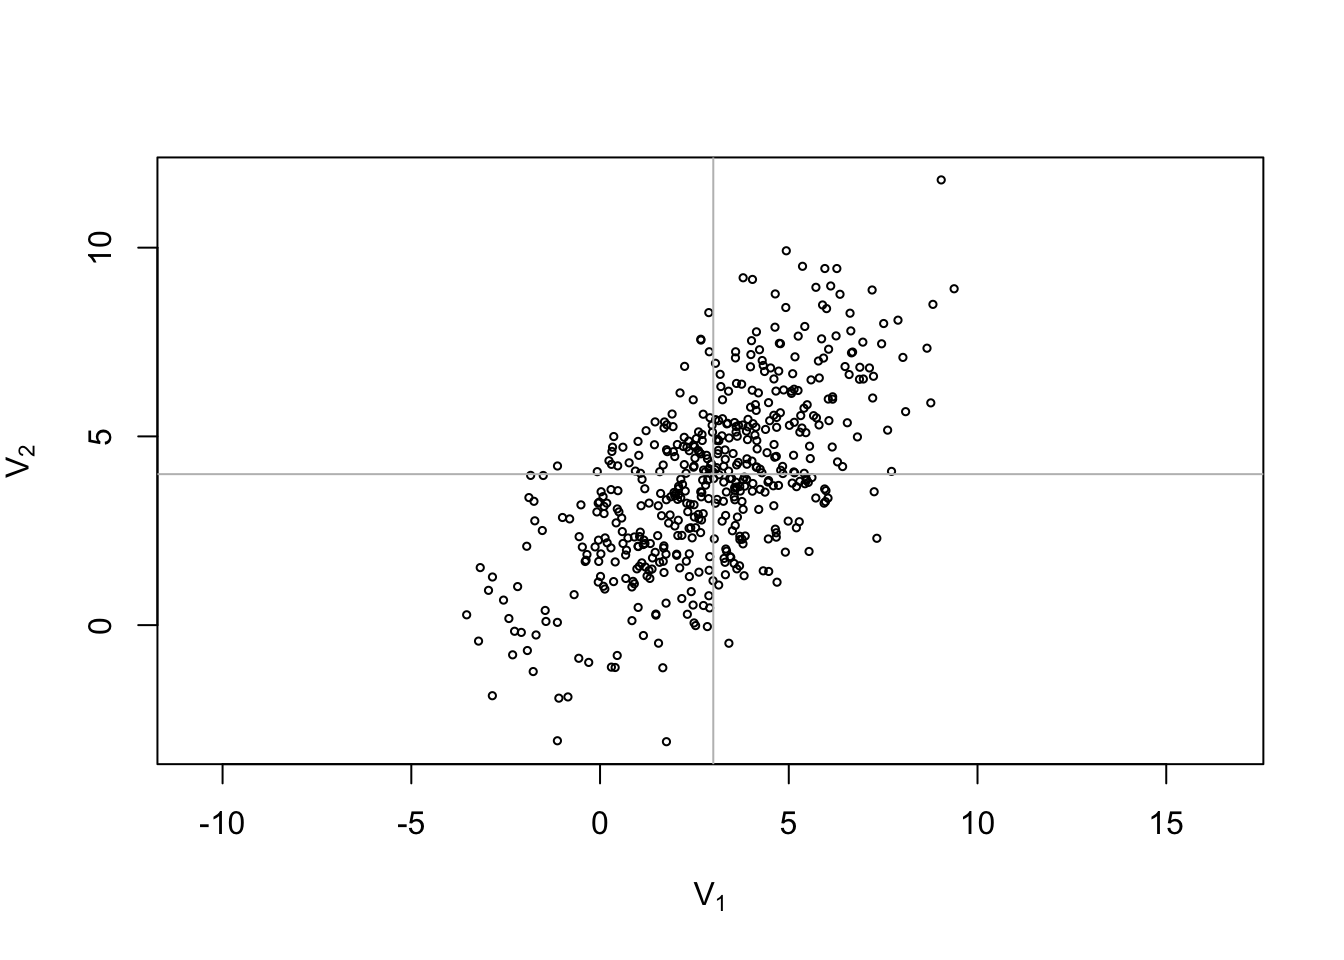
\includegraphics{MATH3714_files/figure-latex/MVN-plot-1.pdf}
\end{example}

\begin{example}
The random vector \(Y\) in \eqref{eq:lmstat0} satisfies \(Y = X \beta + \varepsilon\)
and since \(\varepsilon\sim \mathcal{N}(0, \sigma^2 I)\) we have
\(Y \sim \mathcal{N}(X\beta, \sigma^2 I)\).
\end{example}

\begin{example}
\protect\hypertarget{exm:not-normal}{}\label{exm:not-normal}Let \(Y \sim \mathcal{N}(0, 1)\) be a random variable. Define a random vector
\(Z = (Z_1, Z_2)\) as \(Z_1 = Y\) and
\begin{equation*}
  Z_2 = \begin{cases}
    Y & \mbox{if $|Y|<1$, and}\\
    -Y & \mbox{otherwise.}
  \end{cases}
\end{equation*}
Clearly \(Z_1\) is standard normally distributed.
Since \(\mathcal{N}(0,1)\) is symmetric, both \(Y\) and \(-Y\) are standard normally
distributed and it follows that \(Z_2\) is also standard normally distributed.
Nevertheless, the random vector \(Z\) does not follow a multivariate
normal distribution. Instead of giving a proof of this fact,
we illustrate this here using an R experiment. We start by verifying
that \(Z_1\) and \(Z_2\) are normally distributed.

\begin{Shaded}
\begin{Highlighting}[]
\NormalTok{N }\OtherTok{\textless{}{-}} \DecValTok{1000}
\NormalTok{Y }\OtherTok{\textless{}{-}} \FunctionTok{rnorm}\NormalTok{(N)}
\NormalTok{Z1 }\OtherTok{\textless{}{-}}\NormalTok{ Y}
\NormalTok{Z2 }\OtherTok{\textless{}{-}} \FunctionTok{ifelse}\NormalTok{(}\FunctionTok{abs}\NormalTok{(Y)}\SpecialCharTok{\textless{}}\DecValTok{1}\NormalTok{, Y, }\SpecialCharTok{{-}}\NormalTok{Y)}

\FunctionTok{par}\NormalTok{(}\AttributeTok{mfrow=}\FunctionTok{c}\NormalTok{(}\DecValTok{1}\NormalTok{,}\DecValTok{2}\NormalTok{))}
\FunctionTok{hist}\NormalTok{(Z1, }\AttributeTok{main=}\ConstantTok{NULL}\NormalTok{, }\AttributeTok{xlab=}\FunctionTok{expression}\NormalTok{(Z[}\DecValTok{1}\NormalTok{]))}
\FunctionTok{hist}\NormalTok{(Z2, }\AttributeTok{main=}\ConstantTok{NULL}\NormalTok{, }\AttributeTok{xlab=}\FunctionTok{expression}\NormalTok{(Z[}\DecValTok{2}\NormalTok{]))}
\end{Highlighting}
\end{Shaded}

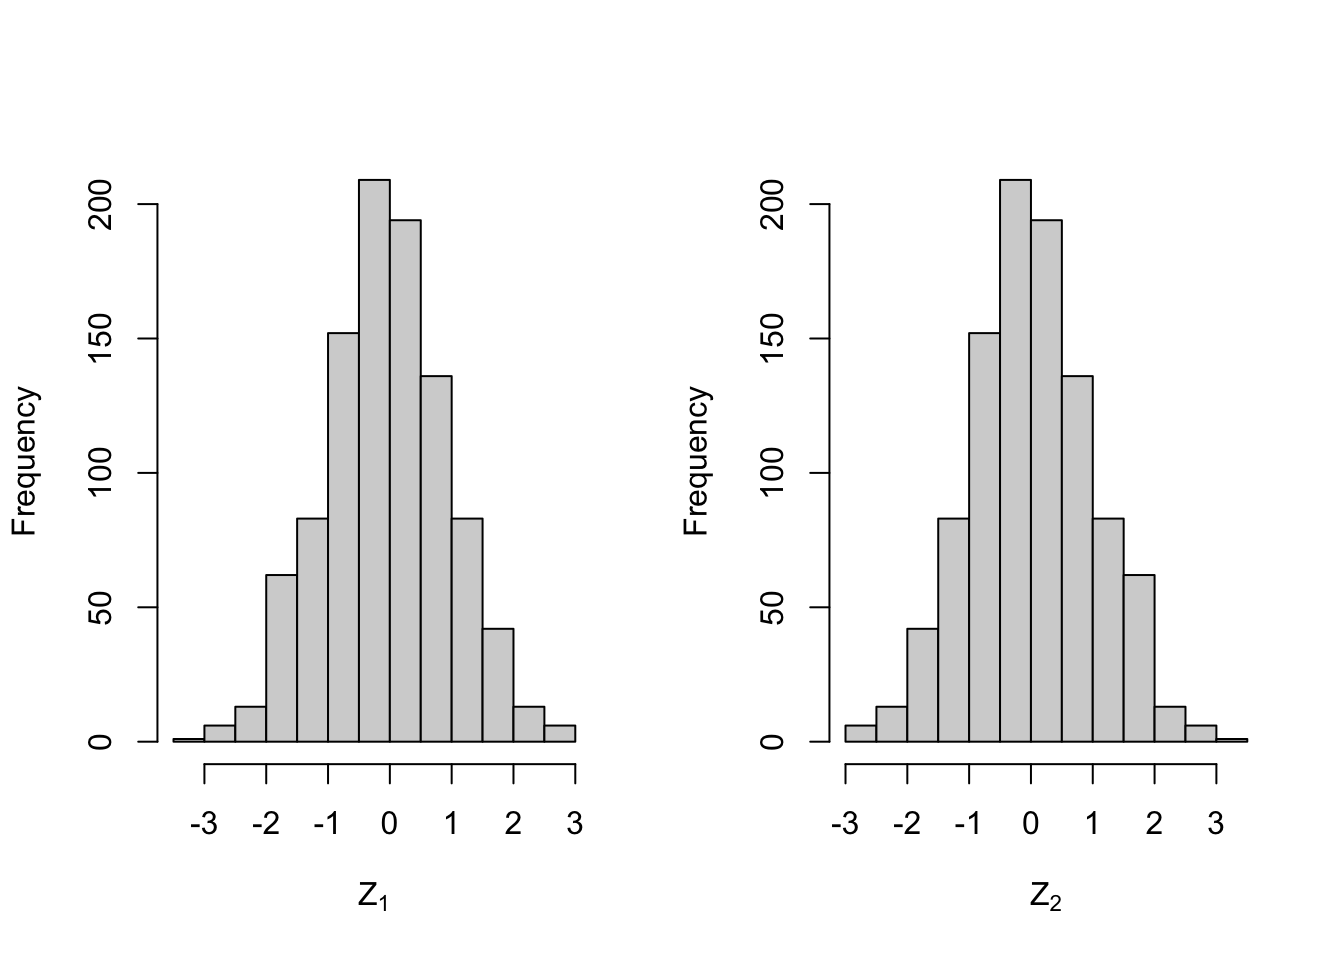
\includegraphics{MATH3714_files/figure-latex/not-a-normal-hist-1.pdf}

The histograms make it plausible that the components are indeed normally
distributed. Now we use a scatter plot to show the joint distribution
of \(Z_1\) and~\(Z_2\):

\begin{Shaded}
\begin{Highlighting}[]
\FunctionTok{plot}\NormalTok{(Z1, Z2, }\AttributeTok{cex=}\FloatTok{0.5}\NormalTok{, }\AttributeTok{asp=}\DecValTok{1}\NormalTok{,}
     \AttributeTok{xlab=}\FunctionTok{expression}\NormalTok{(Z[}\DecValTok{1}\NormalTok{]),}
     \AttributeTok{ylab=}\FunctionTok{expression}\NormalTok{(Z[}\DecValTok{1}\NormalTok{]))}
\end{Highlighting}
\end{Shaded}

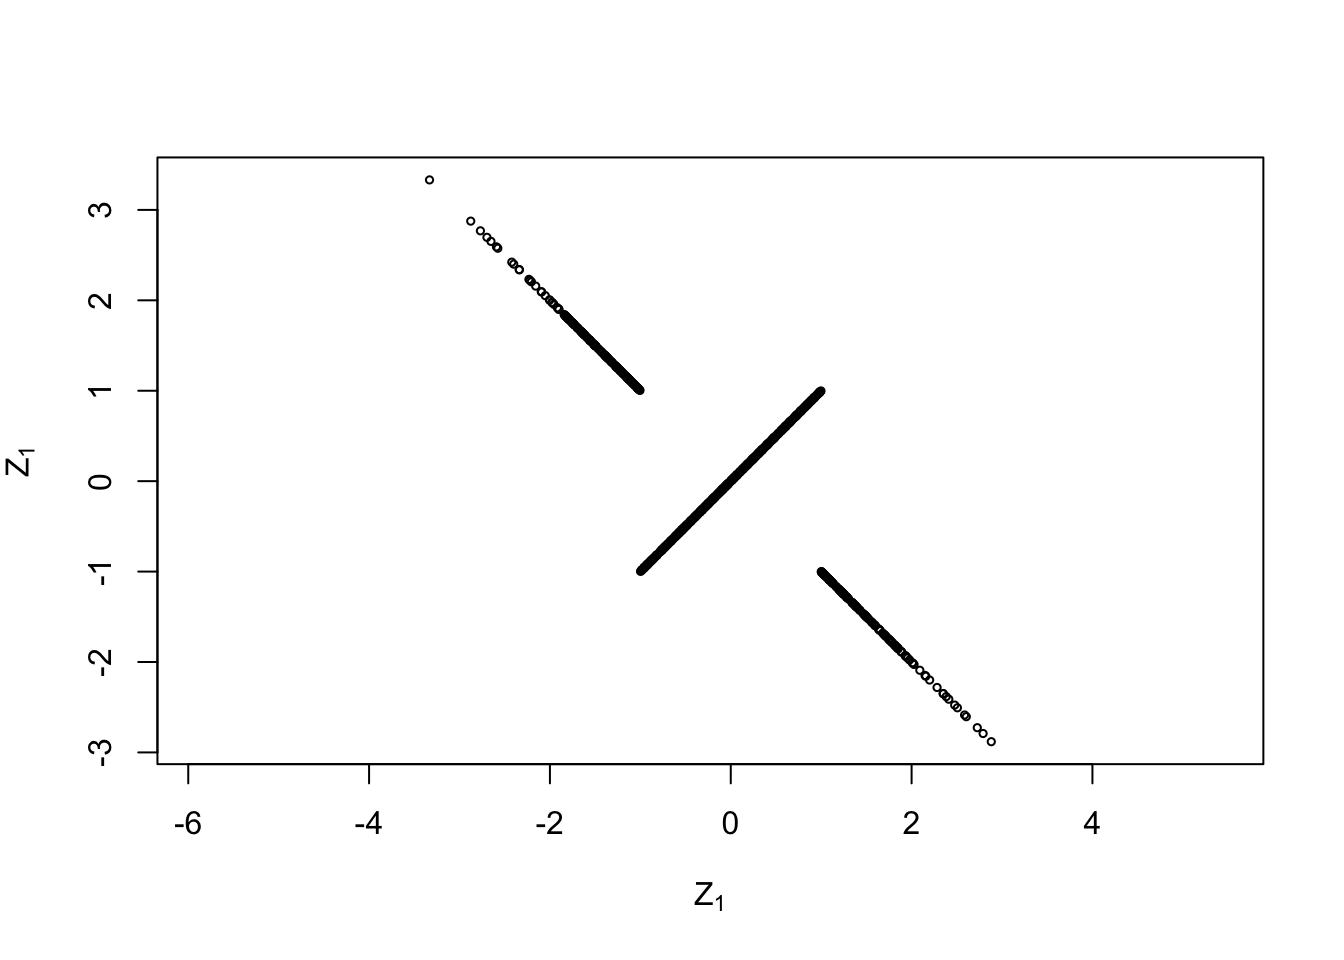
\includegraphics{MATH3714_files/figure-latex/not-a-normal-scatter-1.pdf}

This plot looks peculiar! Most people would not call this a normal distribution
and the formal definition of a multivariate normal distribution is made to
exclude cases like this.
\end{example}

\textbf{Summary}

\begin{itemize}
\tightlist
\item
  We learned the rules for computing the expectation of a random vector.
\item
  The covariance matrix of random vectors plays the role of the
  variance for numeric random variables.
\item
  We learned about the definition of the multivariate normal distribution.
\end{itemize}

\clearpage

\hypertarget{S04-model}{%
\section{Properties of the Least Squares Estimate}\label{S04-model}}

Like in the one-dimensional case, we can build a \textbf{statistical model}
for the data. Here we assume that the residuals are random. More
precisely we have
\begin{equation}
  Y = X \beta + \varepsilon.  \label{eq:lmstats}
\end{equation}
where \(\varepsilon= (\varepsilon_1, \ldots, \varepsilon_n)\) is a random error.
The individual errors \(\varepsilon_1, \ldots, \varepsilon_n\)
are now assumed to be i.i.d.~random variables with \(\mathbb{E}(\varepsilon_i) = 0\) and
\(\mathop{\mathrm{Var}}(\varepsilon_i) = \sigma^2\).

\begin{itemize}
\item
  Again, we assume that the \(x\)-values are fixed and known. The only
  random quantities in the model are \(\varepsilon_i\) and \(Y_i\).
\item
  The parameters in this model are now the regression coefficients
  \(\beta = (\beta_0, \beta_1, \cdots, \beta_p) \in \mathbb{R}^{p+1}\) and
  the error variance~\(\sigma^2\).
\end{itemize}

The usual approach in statistics to quantify how well an estimator works
is to apply it to random samples from the statistical model, where we
can assume that we know the parameters, and then to study how well the
parameters are reconstructed by the estimators. Since this approach
uses random samples as input the the estimator, we obtain random estimates
and we need to use statistical methods to quantify how close the estimate
is to the truth.

\hypertarget{mean-and-covariance}{%
\subsection{Mean and Covariance}\label{mean-and-covariance}}

The bias of an estimator is the difference between the expected value
of the estimate and the truth. For the least squares estimator
we have
\begin{equation*}
  \mathop{\mathrm{bias}}(\hat\beta)
  = \mathbb{E}(\hat\beta) - \beta,
\end{equation*}
where
\begin{equation*}
  \hat\beta
  = (X^\top X)^{-1} X^\top Y
\end{equation*}
and \(Y\) is the random vector from~\eqref{eq:lmstats}.

\begin{lemma}
\protect\hypertarget{lem:hat-beta-dist}{}\label{lem:hat-beta-dist}

We have

\begin{enumerate}
\def\labelenumi{\arabic{enumi})}
\item
  \(\hat\beta = \beta + (X^\top X)^{-1} X^\top \varepsilon\) and
\item
  \(\hat\beta \sim \mathcal{N}\bigl( \beta, \sigma^2 (X^\top X)^{-1} \bigr)\).
\end{enumerate}

\end{lemma}

\begin{proof}
From lemma~\ref{lem:multiple-LSQ} we know
\begin{equation*}
  \hat\beta
  = (X^\top X)^{-1} X^\top Y,
\end{equation*}
Using the definition of \(Y\) we can write this as
\begin{align*}
  \hat\beta
  &= (X^\top X)^{-1} X^\top Y \\
  &= (X^\top X)^{-1} X^\top (X\beta + \varepsilon) \\
  &= (X^\top X)^{-1} X^\top X \beta + (X^\top X)^{-1} X^\top \varepsilon\\
  &= \beta + (X^\top X)^{-1} X^\top \varepsilon.
\end{align*}
This proves the first claim.

Since \(\varepsilon\) follows a multi-variate normal distribution,
\(\beta + (X^\top X)^{-1} X^\top \varepsilon\) is also normally distributed.
Taking expectations we get
\begin{align*}
  \mathbb{E}(\hat\beta)
  &= \mathbb{E}\bigl( \beta + (X^\top X)^{-1} X^\top \varepsilon\bigr) \\
  &= \beta + (X^\top X)^{-1} X^\top \mathbb{E}(\varepsilon) \\
  &= \beta,
\end{align*}
since \(\mathbb{E}(\varepsilon) = 0\).

For the covariance we find
\begin{align*}
  \mathop{\mathrm{Cov}}(\hat\beta)
  &= \mathop{\mathrm{Cov}}\bigl( \beta + (X^\top X)^{-1} X^\top \varepsilon\bigr) \\
  &= \mathop{\mathrm{Cov}}\bigl( (X^\top X)^{-1} X^\top \varepsilon\bigr) \\
  &= (X^\top X)^{-1} X^\top \mathop{\mathrm{Cov}}(\varepsilon) \bigl( (X^\top X)^{-1} X^\top \bigr)^\top \\
  &= (X^\top X)^{-1} X^\top \mathop{\mathrm{Cov}}(\varepsilon) X (X^\top X)^{-1}.
\end{align*}
Since \(\mathop{\mathrm{Cov}}(\varepsilon) = \sigma^2 I\), this simplifies to
\begin{align*}
  \mathop{\mathrm{Cov}}(\hat\beta)
  &= (X^\top X)^{-1} X^\top \sigma^2 I X (X^\top X)^{-1} \\
  &= \sigma^2 (X^\top X)^{-1} X^\top X (X^\top X)^{-1} \\
  &= \sigma^2 (X^\top X)^{-1}.
\end{align*}
This completes the proof.
\end{proof}

The lemma implies that \(\mathbb{E}(\hat\beta) = \beta\), \emph{i.e.}~the estimator
\(\hat\beta\) is unbiased. Note that for this statement we only used \(\mathbb{E}(\varepsilon) = 0\) to compute the expectation of~\(\hat\beta\). Thus, the estimator will still
be unbiases for correlated or for noise which is not normally distributed.

We have seen \protect\hyperlink{eq:Cov-diag-elem}{earlier} that the diagonal elements
of a covariance give the variances of the elements of the random vector.
Setting \(C := (X^\top X)^{-1}\) as a shorthand here, we find that the
individual estimated coefficients \(\hat\beta_i\) satisfy
\begin{equation}
  \hat\beta_i
  \sim \mathcal{N}\bigl( \beta, \sigma^2 C_{ii} \bigr)  \label{eq:beta-hat-i}
\end{equation}
for all \(i \in \{1, \ldots, n\}\).

These results about the (co-)variances of the estimator are not very
useful in practice, because the error variance~\(\sigma^2\) is unknown.
To derive more useful results, we will consider how to estimate this
variance.

\hypertarget{hat-matrix}{%
\subsection{Properties of the Hat Matrix}\label{hat-matrix}}

In this and the following sections we will use various
properties of the hat matrix \(H = X (X^\top X)^{-1} X^\top\).

\begin{lemma}

The hat matrix \(H\) has the following properties:

\begin{enumerate}
\def\labelenumi{\arabic{enumi})}
\tightlist
\item
  \(H\) is symmetric, \emph{i.e.}~\(H^\top = H\).
\item
  \(H\) is idempotent, \emph{i.e.}~\(H^2 = H\).
\end{enumerate}

\end{lemma}

\begin{proof}
For the first statement we have
\begin{align*}
  H^\top
  &= \bigl( X (X^\top X)^{-1} X^\top \bigr)^\top \\
  &= (X^\top)^\top \bigl((X^\top X)^{-1}\bigr)^\top X^\top \\
  &= X (X^\top X)^{-1} X^\top \\
  &= H,
\end{align*}
where we used that the inverse of a symmetric matrix is symmetric.
The second statement follow from
\begin{align*}
  H^2
  &= \bigl( X (X^\top X)^{-1} X^\top \bigr) \bigl( X (X^\top X)^{-1} X^\top \bigr) \\
  &= X \bigl( (X^\top X)^{-1} X^\top X \bigr) (X^\top X)^{-1} X^\top \\
  &= X (X^\top X)^{-1} X^\top.
\end{align*}
This completes the proof.
\end{proof}

Both properties from the lemma carry over from \(H\) to \(I - H\): we
have \((I - H)^\top = I^\top - H^\top = I - H\) and
\begin{align*}
  (I - H)^2
  &= (I - H)(I - H) \\
  &= I^2 - HI - IH + H^2 \\
  &= I - H - H + H \\
  &= I - H.
\end{align*}

For future reference we also state two simpler results: we have
\begin{equation}
  H X = X (X^\top X)^{-1} X^\top X = X  \label{eq:XH}
\end{equation}
and
\begin{equation}
  (I - H) X = IX - HX = X - X = 0.  \label{eq:XIH}
\end{equation}

Finally, if we have a vector \(v \in \mathbb{R}^n\) we can write \(v\) as
\begin{align*}
  v
  &= (H + I - H)v \\
  &= Hv + (I-H)v.
\end{align*}
The inner product between these two components is
\begin{align*}
  (Hv)^\top (I-H)v
  &= v^\top H^\top (I-H) v \\
  &= v^\top H (I-H) v \\
  &= v^\top (H-H^2) v \\
  &= v^\top (H-H) v \\
  &= 0,
\end{align*}
so the two vectors are orthogonal.
As a result we get
\begin{align*}
  \|v\|^2
  &= v^\top v \\
  &= \bigl( Hv + (I-H)v \bigr)^\top \bigl( Hv + (I-H)v \bigr) \\
  &= (Hv)^\top Hv + 2 (Hv)^\top (I-H)v + \bigl((I-H)v\bigr)^\top (I-H)v \\
  &= \| Hv \|^2 + \|(I-H)v \|^2
\end{align*}
(This is \href{https://en.wikipedia.org/wiki/Pythagorean_theorem}{Pythagoras' theorem} in \(\mathbb{R}^n\).)
Since \(\hat y = Hy\) and \(\hat\varepsilon= (I - H)y\), we can apply this idea to the
vector \(y\) of observations to get
\begin{equation}
  \|y\|^2 = \|\hat y\|^2 + \|\hat\varepsilon\|^2.  \label{eq:eps-y-orth}
\end{equation}

We note without proof that geometrically, \(H\) can be interpreted as the
orthogonal projection onto the subspace of \(\mathbb{R}^n\) which is spanned by
the columns of \(X\). This subspace contains the possible output vectors
of the linear system and the least squares procedure finds the point \(\hat y\)
in this subspace which is closest to the observed data \(y\in\mathbb{R}^n\).

Some authors define:

\begin{itemize}
\tightlist
\item
  \(\mathrm{SS}_\mathrm{T} = \sum_{i=1}^n y_i^2\) (where ``T'' stands for ``total'')
\item
  \(\mathrm{SS}_\mathrm{R} = \sum_{i=1}^n \hat y_i^2\) (where ``R'' stands for ``regression'')
\item
  \(\mathrm{SS}_\mathrm{E} = \sum_{i=1}^n \hat\varepsilon_i^2 = \sum_{i=1}^n (y_i-\hat y_i)^2\) (where ``E'' stands for ``error'')
\end{itemize}

Using this notation, our equation
\(\|y\|^2 = \|\hat y\|^2 + \|\hat\varepsilon\|^2\)
turns into
\begin{equation*}
  \mathrm{SS}_\mathrm{T}
  = \mathrm{SS}_\mathrm{R} + \mathrm{SS}_\mathrm{E}.
\end{equation*}

\hypertarget{Cochran}{%
\subsection{Cochran's theorem}\label{Cochran}}

Our main tool in this and the following section will be a simplified
version of \href{https://en.wikipedia.org/wiki/Cochran\%27s_theorem}{Cochran's theorem}.

\begin{theorem}
\protect\hypertarget{thm:Cochran}{}\label{thm:Cochran}

The following statements are true:

\begin{enumerate}
\def\labelenumi{\arabic{enumi})}
\item
  \(\frac{1}{\sigma^2} \varepsilon^\top H \varepsilon\sim \chi^2(p+1)\)
\item
  \(\frac{1}{\sigma^2} \varepsilon^\top (I - H) \varepsilon\sim \chi^2(n - p - 1)\)
\item
  \(H \varepsilon\) and \((I-H)\varepsilon\) are independent.
\end{enumerate}

\end{theorem}

\begin{proof}
Since \(H\) is symmetric, we can diagonalise \(H\) (see \ref{thm:spectral}
in the appendix): there is an orthogonal matrix \(U\) such that
\(D := U H U^\top\) is diagonal, and the diagonal elements of \(D\) are
the eigenvalues of \(H\). Since \(H\) is idempotent, these diagonal elements
can only be \(0\) or~\(1\). Also, since \(U\) is orthogonal, we have \(U^\top U = I\)
and thus
\begin{equation*}
  U^\top D U
  = U^\top U H U^\top U
  = H.
\end{equation*}
The same matrix \(U\) also diagonalises \(I-H\), since
\(U (I -H) U^\top = U U^\top - U H U^\top = I - D\). Exactly one
of the diagonal elements \(D_{ii}\) and \((I - D)_{ii}\) is \(1\) and the other
one is \(0\) for every~\(i\).

Since \(\varepsilon\sim \mathcal{N}(0, \sigma^2 I)\) we find that \(\eta := U \varepsilon\) is normally
distributed with mean \(U 0 = 0\) and covariance matrix \(\sigma^2 U I U^\top = \sigma^2 U U^\top = \sigma^2 I\). Thus \(\eta\) has the same distribution as
\(\varepsilon\) does: \(\eta \sim \mathcal{N}(0, \sigma^2I)\) and the components \(\eta_i\)
are independent of each other. We have
\begin{equation*}
  H \varepsilon
  = U^\top D U \varepsilon
  = U^\top D \eta.
\end{equation*}
and
\begin{equation*}
  (I - H) \varepsilon
  = U^\top (I - D) U \varepsilon
  = U^\top (I - D) \eta.
\end{equation*}
Since \((D\eta)_i = 0\) if \(D_{ii}=0\) and \(\bigl((I - D) \eta)_i = 0\)
otherwise, each component of \(\eta\) contributes to exactly one of the
two vectors \(D\eta\) and \((I-D)\eta\). Thus, \(D\eta\) and \((I-D)\eta\)
are independent, and thus \(H\varepsilon\) and \((I - H)\varepsilon\) are also independent.
This proves the third statement of the theorem.

For the first statement, we note that
\begin{align*}
  \varepsilon^\top H \varepsilon
  &= \varepsilon^\top U^\top D U \varepsilon\\
  &= \eta^\top D \eta \\
  &= \sum_{i=1 \atop D_{ii}=1}^n \eta_i^2.
\end{align*}
Since \((X^\top X) \in\mathbb{R}^{(p+1)\times (p+1)}\) is invertible, one can show
that \(\mathop{\mathrm{rank}}(H) = p+1\) and thus that there are \(p+1\) terms contributing
to the sum (we skip the proof of this statement here). Thus,
\begin{equation*}
  \frac{1}{\sigma^2} \varepsilon^\top H \varepsilon
  = \sum_{i=1 \atop D_{ii}=1}^n \bigl(\eta_i/\sigma)^2
\end{equation*}
is the sum of the squares of \(p+1\) independent standard normals,
and thus is \(\chi^2(p+1)\) distributed. This completes the proof of the
first statement.

Finally, the second statement follows in much of the same way as the
first one, except that \(H\) is replaced with \(I-H\) and the sum is
over the \(n - p - 1\) indices \(i\) where \(D_{ii} = 0\).
This completes the proof.
\end{proof}

Expressions of the form \(x^\top A x\) for \(x\in\mathbb{R}^n\) and \(A\in\mathbb{R}^{n\times n}\)
are called \textbf{quadratic forms}.

While the theorem as written only states that \(H \varepsilon\) and \((I - H)\varepsilon\)
are independent of each other, we can replace one or both of these terms
the corresponding quadratic forms as still keep the independence. Since
\((H \varepsilon)^\top (H \varepsilon) = \varepsilon^\top H^\top H \varepsilon= \varepsilon^\top H \varepsilon\),
the quadratic form \(\varepsilon^\top H \varepsilon\) is a function of \(H \varepsilon\) and a similar
statement holds with \(H-I\) instead of \(H\).

\hypertarget{var-est-bias}{%
\subsection{Estimating the Error Variance}\label{var-est-bias}}

So far we have only considered how to estimate the parameter
vector~\(\beta\) and we have ignored the parameter~\(\sigma^2\).
We will see that an unbiased estimator for \(\sigma^2\) is
given by
\begin{equation}
  \hat\sigma^2
  := \frac{1}{n-p-1} \sum_{i=1}^n (y_i - \hat y_i)^2, \label{eq:hat-sigma-squared}
\end{equation}
where \(\hat y_i\) are the fitted values from equation~\eqref{eq:fitted-values}.
As for the one-dimensional case in~\eqref{eq:reg-sigma-est}, the estimate
does not have the prefactor \(1/n\), which one might naively expect,
but the denomintor is decreased by one for each component of the
vector~\(\beta\). Using Cochran's theorem, we can now show that the estimator
\(\hat\sigma^2\) is unbiased.

We first note that
\begin{align*}
  (n - p - 1) \hat\sigma^2
  &= (y - \hat y)^\top (y - \hat y) \\
  &= (y - H y)^\top (y - H y) \\
  &= y^\top (I - H)^\top (I - H) y \\
  &= y^\top (I - H) y
\end{align*}
To determine the bias, we need to use \(Y = X\beta + \varepsilon\) in place of the
data. This gives
\begin{align*}
  (n - p - 1) \hat\sigma^2
  &= Y^\top (I-H) Y \\
  &= (X\beta + \varepsilon)^\top (I-H) (X\beta + \varepsilon) \\
  &= \beta^\top X^\top (I-H) X \beta
      + 2 \varepsilon^\top (I-H) X \beta
      + \varepsilon^\top (I-H) \varepsilon\\
  &= \varepsilon^\top (I-H) \varepsilon,
\end{align*}
where we used equation~\eqref{eq:XIH} to see that the first two terms in
the sum equal zero.

Now we can apply Cochran's theorem. This shows that
\begin{equation}
  \frac{1}{\sigma^2} (n - p - 1) \hat\sigma^2
  = \frac{1}{\sigma^2} \varepsilon^\top (I-H) \varepsilon
  \sim \chi^2(n - p - 1).  \label{eq:sigma-hat-chi-squared}
\end{equation}
Since the expectation of a \(\chi^2(\nu)\) distribution equals \(\nu\)
(see appendix~\ref{chi-square}), we find
\begin{equation*}
  \frac{1}{\sigma^2} (n - p - 1) \mathbb{E}(\hat\sigma^2)
  = n - p - 1
\end{equation*}
and thus
\begin{equation*}
  \mathbb{E}(\hat\sigma^2)
  = \sigma^2.
\end{equation*}
This proves that \(\hat\sigma^2\) is an unbiased estimator for \(\sigma^2\).

\textbf{Summary}

\begin{itemize}
\tightlist
\item
  The least squares estimator for the regression coefficients is unbiased.
\item
  The hat matrix is idempotent and symmetric.
\item
  Cochran's theorem allows to understand the distribution of some
  quadratic forms involving the hat matrix.
\item
  \(\hat\sigma^2\) is an unbiased estimator for \(\sigma^2\).
\end{itemize}

\clearpage

\hypertarget{S05-single}{%
\section{Uncertainty for Individual Regression Coefficients}\label{S05-single}}

In this section we will consider different ways to study the uncertainty in the
estimates \(\hat\beta_i\) for the regression coefficient~\(\beta_i\),
individually. In the following sections we will then consider the problem of
simultaneously estimating several or all coefficients.

\hypertarget{measuring-the-estimation-error}{%
\subsection{Measuring the Estimation Error}\label{measuring-the-estimation-error}}

We have seen that \(\hat\beta \sim \mathcal{N}(\beta, \sigma^2 C)\), where
\(C := (X^\top X)^{-1}\). Restricting this to a single coefficient, we find
\begin{equation*}
  \hat\beta_i
  \sim \mathcal{N}\bigl( \beta_i, \sigma^2 C_{ii} \bigr),
\end{equation*}
since the diagonal elements of the covariance matrix contains the
variances of the elements of a random vector. In practice we will not
know the value of \(\sigma^2\), so we have to estimate this from data,
using the estimator
\begin{equation*}
  \hat\sigma^2
  = \frac{1}{n-p-1} \sum_{i=1}^n (y_i - \hat y_i)^2,
\end{equation*}
from equation~\eqref{eq:hat-sigma-squared}. As a first application of
Cochran's theorem we showed in equation~\eqref{eq:sigma-hat-chi-squared}
that
\begin{equation*}
  \frac{1}{\sigma^2} (n - p - 1) \hat\sigma^2
  \sim \chi^2(n - p - 1).
\end{equation*}

Note that in the equations above, we index the rows and columns of \(C\)
using \(i,j\in \{0, 1, \ldots, p\}\), \emph{i.e.} the first row and column are
using the index 0 each. This is to match the convention for the
components of \(\beta = (\beta_0, \beta_1, \ldots, \beta_p)\).

\begin{lemma}
\protect\hypertarget{lem:hat-beta-sigma-indep}{}\label{lem:hat-beta-sigma-indep}The random vector \(\hat\beta\) and the random number
\(\hat\sigma^2\) are independent of each other.
\end{lemma}

\begin{proof}
We will show that \(\hat\beta\) can be written as a function of \(H\varepsilon\)
and that \(\hat\sigma^2\) can be written as a function of \((I-H)\varepsilon\).
The result then follows from Cochran's theorem.

From lemma~\ref{lem:hat-beta-dist}
we know that the least squares estimate \(\hat\beta\) can be written as
\begin{equation*}
  \hat\beta
  = \beta + (X^\top X)^{-1} X^\top \varepsilon
\end{equation*}
and that \(H = X (X^\top X)^{-1} X^\top\). Thus we can write \(\hat\beta\) as
\begin{align*}
  \hat\beta
  &= \beta + (X^\top X)^{-1} X^\top X \, (X^\top X)^{-1} X^\top \varepsilon\\
  &= \beta + (X^\top X)^{-1} X^\top H \varepsilon,
\end{align*}
which is a function of \(H\varepsilon\).

Similar to the argument at the end of the previous section, we can
write \(\hat\sigma^2\) as
\begin{align*}
  (n - p - 1) \hat\sigma^2
  &= (Y - \hat Y)^\top (Y - \hat Y) \\
  &= (Y - H Y)^\top (Y - H Y) \\
  &= Y^\top (I - H)^\top (I - H) Y \\
  &= \bigl\| (I - H) Y \|.
\end{align*}
Since \(Y = X\beta + \varepsilon\) and since we know \((I-H)X = 0\) from
equation~\eqref{eq:XIH}, we find
\begin{align*}
  \hat\sigma^2
  &= \frac{1}{n-p-1} \bigl\| (I - H) (X\beta + \varepsilon) \| \\
  &= \frac{1}{n-p-1} \bigl\| (I - H) \varepsilon\|,
\end{align*}
which is a function of \((I - H)\varepsilon\).

From Cochran's theorem we know that \(H \varepsilon\) and \((I-H)\varepsilon\) are independent
and thus we can conclude that \(\hat\beta\) and \(\hat\sigma^2\) are also
independent of each other. This completes the proof.
\end{proof}

We now construct a quantity \(T\) which measures the distance between
the estimated value \(\hat\beta_i\) and the unknown true value~\(\beta_i\):
\begin{equation}
  T
  := \frac{\hat\beta_i - \beta_i}{\sqrt{\hat\sigma^2 C_{ii}}}. \label{eq:single-T}
\end{equation}
While there are many ways to measure this distance, the \(T\) constructed
here has two main advantages:

\begin{itemize}
\item
  The value of \(T\) can be computed from the given data, without
  any reference to unknown quantities.
\item
  Below, we will be able to find the distribution of \(T\). This will
  allow us to use \(T\) to construct confidence intervals and statistical
  tests.
\end{itemize}

\begin{lemma}
\protect\hypertarget{lem:beta-i-follows-t}{}\label{lem:beta-i-follows-t}Assume that the data follows the model~\eqref{eq:lmstats}.
Then \(T \sim t(n-p-1)\), \emph{i.e.} \(T\) follows a
\(t\)-distribution with \(n-p-1\) degrees of freedom (see appendix \ref{t}).
\end{lemma}

\begin{proof}
We have
\begin{align*}
  T
  &= \frac{(\hat\beta_i - \beta_i) / \sqrt{C_{ii}}}
      {\sqrt{\hat\sigma^2}} \\
  &= \frac{(\hat\beta_i - \beta_i) / \sqrt{\sigma^2 C_{ii}}}
      {\sqrt{\hat\sigma^2 / \sigma^2}} \\
  &= \frac{(\hat\beta_i - \beta_i) / \sqrt{\sigma^2 C_{ii}}}
      {\sqrt{((n - p - 1) \hat\sigma^2 / \sigma^2) / (n - p -1)}} \\
  &=: \frac{Z}{\sqrt{Y / (n - p - 1)}},
\end{align*}
where \(Z = (\hat\beta_i - \beta_i) / \sqrt{\sigma^2 C_{ii}} \sim \mathcal{N}(0,1)\)
and \(Y = (n - p - 1) \hat\sigma^2/\sigma^2 \sim \chi^2(n-p-1)\)
are independent, by lemma~\ref{lem:hat-beta-sigma-indep}.
Thus, \(T \sim t(n-p-1)\) as required.
\end{proof}

The quantity \(\sqrt{\sigma^2 C_{ii}}\) is sometimes called the
\textbf{standard error} of the estimator \(\hat\beta_i\), denoted by
\(\mathop{\mathrm{se}}(\hat\beta_i)\).

\hypertarget{confidence-intervals}{%
\subsection{Confidence Intervals}\label{confidence-intervals}}

Using the scaled distance~\(T\), it is easy to construct a confidence
interval for \(\hat\beta_i\): For \(\alpha \in (0, 1)\), say \(\alpha = 5\%\),
lemma~\ref{lem:beta-i-follows-t} shows that
\begin{equation*}
  P\Bigl( T \in \bigl[-t_{n-p-1}(\alpha/2), +t_{n-p-1}(\alpha/2)\bigr] \Bigr)
  = 1 - \alpha,
\end{equation*}
where \(t_{n-p-1}(\alpha/2)\) is the \((1 - \alpha/2)\)-quantile of the
\(t(n-p-1)\)-distribution. Rewriting this expression as a condition on
\(\hat\beta_i\) instead of on \(T\) gives a confidence interval for \(\beta_i\).

\begin{lemma}
\protect\hypertarget{lem:single-CI}{}\label{lem:single-CI}The interval
\begin{equation*}
  [U, V]
  := \Bigl[ \hat\beta_i - \sqrt{\hat\sigma^2 C_{ii}}t_{n-p-1}(\alpha/2), \hat\beta_i + \sqrt{\hat\sigma^2 C_{ii}}t_{n-p-1}(\alpha/2) \Bigr]
\end{equation*}
is a \((1-\alpha)\)-confidence interval for~\(\beta_i\).
\end{lemma}

\begin{proof}
We have to show that \(P(\beta_i \in [U, V]) \geq 1-\alpha\). We have
\begin{align*}
  &\hskip-5mm \beta_i \in [U, V] \\
  &\Longleftrightarrow
    \bigl| \hat\beta_i - \beta_i \bigr|
        \leq \sqrt{\hat\sigma^2 C_{ii}}t_{n-p-1}(\alpha/2) \\
  &\Longleftrightarrow
    \Bigl| \frac{\hat\beta_i - \beta_i}{\sqrt{\hat\sigma^2 C_{ii}}} \Bigr|
        \leq t_{n-p-1}(\alpha/2) \\
  &\Longleftrightarrow
    T \in \bigl[-t_{n-p-1}(\alpha/2), +t_{n-p-1}(\alpha/2)\bigr]
\end{align*}
and thus \(P(\beta_i \in [U, V]) = 1 - \alpha\). This completes the proof.
\end{proof}

\hypertarget{hypthesis-tests}{%
\subsection{Hypthesis Tests}\label{hypthesis-tests}}

Very similar to the argument for confidence intervals, we can
derive a hypothesis test to test the hypothesis
\begin{equation*}
  H_0\colon \beta_i = b
\end{equation*}
against the alternative
\begin{equation*}
  H_1\colon \beta_i \neq b.
\end{equation*}

Here we redefine \(T\) as
\begin{equation}
  T
  := \frac{\hat\beta_i - b}{\sqrt{\hat\sigma^2 C_{ii}}},  \label{eq:single-test}
\end{equation}
using \(b\) in place of the \(\beta_i\) above. When \(H_0\) is true, this new
defintion of \(T\) is the same as~\eqref{eq:single-T}.

\begin{lemma}
\protect\hypertarget{lem:t-test}{}\label{lem:t-test}The test which rejects \(H_0\) if and only if \(|T| > t_{n-p-1}(\alpha/2)\)
has significance level~\(\alpha\).
\end{lemma}

\begin{proof}
We have to show that the probability of type~I errors (\emph{i.e.} of wrongly
rejecting \(H_0\) when it is true) is less than or equal to~\(\alpha\).
Assume that \(H_0\) is true. Then we have \(\beta_i = b\) and thus
the \(T\) defined in this section coincides with the expression from
equation~\eqref{eq:single-T}. From lemma~\ref{lem:beta-i-follows-t}
we know that \(T \sim t(n-p-1)\). Thus we have
\begin{align*}
  P( \mbox{type I error} )
  &= P\bigl( |T| > t_{n-p-1}(\alpha/2) \bigr) \\
  &= P\bigl(T < -t_{n-p-1}(\alpha/2) \bigr) + P\bigl(T > t_{n-p-1}(\alpha/2) \bigr) \\
  &= 2 P\bigl(T > t_{n-p-1}(\alpha/2) \bigr) \\
  &= 2 P\bigl(T > t_{n-p-1}(\alpha/2) \bigr) \\
  &= 2 \frac{\alpha}{2} \\
  &= \alpha.
\end{align*}
This completes the proof.
\end{proof}

If we use \(b = 0\) in the test, we can test whether \(\beta_i = 0\).
If \(\beta_i = 0\) is true, the corresponding input \(x_i\) has no influence
on the output.

As usual with statistical tests, one needs to be extremely careful when
performing several tests on the same data. In particular, it would be
unwise to test more than one component of \(\beta\) using this procedure
for the same data. Instead, in the next section we will consider how
to perform tests for several components of \(\beta\) simultaneously.
Before we do this, we will perform some experiments with R.

\hypertarget{r-experiments}{%
\subsection{R Experiments}\label{r-experiments}}

\hypertarget{fitting-the-model}{%
\subsubsection{Fitting the model}\label{fitting-the-model}}

\begin{Shaded}
\begin{Highlighting}[]
\NormalTok{m }\OtherTok{\textless{}{-}} \FunctionTok{lm}\NormalTok{(stack.loss }\SpecialCharTok{\textasciitilde{}}\NormalTok{ ., }\AttributeTok{data =}\NormalTok{ stackloss)}
\FunctionTok{summary}\NormalTok{(m)}
\end{Highlighting}
\end{Shaded}

\begin{Shaded}
\begin{Highlighting}[]
\NormalTok{\# }
\NormalTok{\# Call:}
\NormalTok{\# lm(formula = stack.loss \textasciitilde{} ., data = stackloss)}
\NormalTok{\# }
\NormalTok{\# Residuals:}
\NormalTok{\#     Min      1Q  Median      3Q     Max }
\NormalTok{\# {-}7.2377 {-}1.7117 {-}0.4551  2.3614  5.6978 }
\NormalTok{\# }
\NormalTok{\# Coefficients:}
\NormalTok{\#             Estimate Std. Error t value Pr(\textgreater{}|t|)    }
\NormalTok{\# (Intercept) {-}39.9197    11.8960  {-}3.356  0.00375 ** }
\NormalTok{\# Air.Flow      0.7156     0.1349   5.307  5.8e{-}05 ***}
\NormalTok{\# Water.Temp    1.2953     0.3680   3.520  0.00263 ** }
\NormalTok{\# Acid.Conc.   {-}0.1521     0.1563  {-}0.973  0.34405    }
\NormalTok{\# {-}{-}{-}}
\NormalTok{\# Signif. codes:  0 \textquotesingle{}***\textquotesingle{} 0.001 \textquotesingle{}**\textquotesingle{} 0.01 \textquotesingle{}*\textquotesingle{} 0.05 \textquotesingle{}.\textquotesingle{} 0.1 \textquotesingle{} \textquotesingle{} 1}
\NormalTok{\# }
\NormalTok{\# Residual standard error: 3.243 on 17 degrees of freedom}
\NormalTok{\# Multiple R{-}squared:  0.9136,  Adjusted R{-}squared:  0.8983 }
\NormalTok{\# F{-}statistic:  59.9 on 3 and 17 DF,  p{-}value: 3.016e{-}09}
\end{Highlighting}
\end{Shaded}

\hypertarget{estimating-the-variance-of-the-error}{%
\subsubsection{Estimating the Variance of the Error}\label{estimating-the-variance-of-the-error}}

We can get the design matrix \(X\) and the covariance matrix \(C\) as follows:

\begin{Shaded}
\begin{Highlighting}[]
\NormalTok{X }\OtherTok{\textless{}{-}} \FunctionTok{model.matrix}\NormalTok{(m)}
\NormalTok{C }\OtherTok{\textless{}{-}} \FunctionTok{solve}\NormalTok{(}\FunctionTok{t}\NormalTok{(X) }\SpecialCharTok{\%*\%}\NormalTok{ X)}
\FunctionTok{round}\NormalTok{(C, }\DecValTok{4}\NormalTok{)}
\end{Highlighting}
\end{Shaded}

\begin{Shaded}
\begin{Highlighting}[]
\NormalTok{\#             (Intercept) Air.Flow Water.Temp Acid.Conc.}
\NormalTok{\# (Intercept)     13.4527   0.0273    {-}0.0620    {-}0.1594}
\NormalTok{\# Air.Flow         0.0273   0.0017    {-}0.0035    {-}0.0007}
\NormalTok{\# Water.Temp      {-}0.0620  {-}0.0035     0.0129     0.0000}
\NormalTok{\# Acid.Conc.      {-}0.1594  {-}0.0007     0.0000     0.0023}
\end{Highlighting}
\end{Shaded}

Next we need to estimate the variance \(\sigma^2\):

\begin{Shaded}
\begin{Highlighting}[]
\NormalTok{y }\OtherTok{\textless{}{-}}\NormalTok{ stackloss}\SpecialCharTok{$}\NormalTok{stack.loss}
\NormalTok{n }\OtherTok{\textless{}{-}} \FunctionTok{nrow}\NormalTok{(stackloss)}
\NormalTok{p }\OtherTok{\textless{}{-}} \FunctionTok{ncol}\NormalTok{(stackloss) }\SpecialCharTok{{-}} \DecValTok{1}
\NormalTok{hat.sigma2 }\OtherTok{\textless{}{-}} \FunctionTok{sum}\NormalTok{((y }\SpecialCharTok{{-}} \FunctionTok{fitted}\NormalTok{(m))}\SpecialCharTok{\^{}}\DecValTok{2}\NormalTok{) }\SpecialCharTok{/}\NormalTok{ (n }\SpecialCharTok{{-}}\NormalTok{ p }\SpecialCharTok{{-}} \DecValTok{1}\NormalTok{)}
\NormalTok{hat.sigma2}
\end{Highlighting}
\end{Shaded}

\begin{Shaded}
\begin{Highlighting}[]
\NormalTok{\# [1] 10.51941}
\end{Highlighting}
\end{Shaded}

The square root of this number, so the estimated standard deviation of the
\(\varepsilon_i\) is shown as \texttt{Residual\ standard\ error} in the summary output above.
We check that we get the same result:

\begin{Shaded}
\begin{Highlighting}[]
\FunctionTok{sqrt}\NormalTok{(hat.sigma2)}
\end{Highlighting}
\end{Shaded}

\begin{Shaded}
\begin{Highlighting}[]
\NormalTok{\# [1] 3.243364}
\end{Highlighting}
\end{Shaded}

This result is also listed as the \texttt{Residual\ standard\ error} near the
bottom of the \texttt{summary(m)} output, above.

\hypertarget{estimating-the-standard-errors}{%
\subsubsection{Estimating the Standard Errors}\label{estimating-the-standard-errors}}

We can the standard errors, \emph{i.e.}~the standard deviations
\(\mathop{\mathrm{stdev}}(\hat\beta)_i\) as \(\sqrt{\hat\sigma^2 C_{ii}}\):

\begin{Shaded}
\begin{Highlighting}[]
\NormalTok{se }\OtherTok{\textless{}{-}} \FunctionTok{sqrt}\NormalTok{(hat.sigma2 }\SpecialCharTok{*} \FunctionTok{diag}\NormalTok{(C))}
\NormalTok{se}
\end{Highlighting}
\end{Shaded}

\begin{Shaded}
\begin{Highlighting}[]
\NormalTok{\# (Intercept)    Air.Flow  Water.Temp  Acid.Conc. }
\NormalTok{\#  11.8959969   0.1348582   0.3680243   0.1562940}
\end{Highlighting}
\end{Shaded}

These values are also listed in the \texttt{Std.\ Error} column of the \texttt{summary(m)}
output.

\hypertarget{hypothesis-tests}{%
\subsubsection{Hypothesis tests}\label{hypothesis-tests}}

Let us now test the hypothesis \(H_0\colon \beta_i = 0\). The test statistic
for this case is the following:

\begin{Shaded}
\begin{Highlighting}[]
\NormalTok{T }\OtherTok{\textless{}{-}} \FunctionTok{coef}\NormalTok{(m) }\SpecialCharTok{/}\NormalTok{ se}
\NormalTok{T}
\end{Highlighting}
\end{Shaded}

\begin{Shaded}
\begin{Highlighting}[]
\NormalTok{\# (Intercept)    Air.Flow  Water.Temp  Acid.Conc. }
\NormalTok{\#  {-}3.3557234   5.3066130   3.5195672  {-}0.9733098}
\end{Highlighting}
\end{Shaded}

These values are also listed in the \texttt{t\ value} column of the \texttt{summary(m)}
output.

Before we can perform the test, we need to choose \(\alpha\) and to
find the corresponding critical value:

\begin{Shaded}
\begin{Highlighting}[]
\NormalTok{alpha }\OtherTok{\textless{}{-}} \FloatTok{0.05}
\NormalTok{t }\OtherTok{\textless{}{-}} \FunctionTok{qt}\NormalTok{(}\DecValTok{1} \SpecialCharTok{{-}}\NormalTok{ alpha}\SpecialCharTok{/}\DecValTok{2}\NormalTok{ , n }\SpecialCharTok{{-}}\NormalTok{ p }\SpecialCharTok{{-}} \DecValTok{1}\NormalTok{)}
\NormalTok{t}
\end{Highlighting}
\end{Shaded}

\begin{Shaded}
\begin{Highlighting}[]
\NormalTok{\# [1] 2.109816}
\end{Highlighting}
\end{Shaded}

Using the critical value \(t\) we can decided whether \(H_0\) should be accepted or
rejected. For example, looking at the intercept \(\beta_0\), we find \(|T_0| = |-3.3557234| > 2.109816 = t_{n-p-1}(1-\alpha/2)\) and thus we can reject the
hypothesis \(H_0\colon \beta_0 = 0\). This means that the intercept is
significantly different from 0.

\hypertarget{confidence-intervals-1}{%
\subsubsection{Confidence Intervals}\label{confidence-intervals-1}}

Using the quantile \texttt{t} we can also get confidence intervals. Here we
only show the confidence interval for the intercept \(\beta_0\):

\begin{Shaded}
\begin{Highlighting}[]
\FunctionTok{c}\NormalTok{(}\FunctionTok{coef}\NormalTok{(m)[}\DecValTok{1}\NormalTok{] }\SpecialCharTok{{-}}\NormalTok{ se[}\DecValTok{1}\NormalTok{] }\SpecialCharTok{*}\NormalTok{ t, }\FunctionTok{coef}\NormalTok{(m)[}\DecValTok{1}\NormalTok{] }\SpecialCharTok{+}\NormalTok{ se[}\DecValTok{1}\NormalTok{] }\SpecialCharTok{*}\NormalTok{ t)}
\end{Highlighting}
\end{Shaded}

\begin{Shaded}
\begin{Highlighting}[]
\NormalTok{\# (Intercept) (Intercept) }
\NormalTok{\#   {-}65.01803   {-}14.82131}
\end{Highlighting}
\end{Shaded}

Confidence intervals for the remaining coefficients can be obtained simimlarly.

\textbf{Summary}

\begin{itemize}
\tightlist
\item
  We know how to scale the distance between individual parameter estimates
  and the truth.
\item
  We have seen how to construct confidence intervals for \(\beta_i\).
\item
  We have seen how to construct statistical tests for \(\beta_i\).
\item
  We have understood some more of the summary output for the \texttt{lm()}
  function in~R.
\end{itemize}

\clearpage

\hypertarget{S06-simultaneous}{%
\section{Estimating Coefficients Simultaneously}\label{S06-simultaneous}}

In this section we will study how to assess the uncertainty in two or more
regression coefficients simultaneously. This is needed since the estimates for
different coefficients will usually not be independent.

\hypertarget{sec:simult-dist}{%
\subsection{Linear Combinations of Coefficients}\label{sec:simult-dist}}

As a general setup which allows to describe which coefficients we are
interested in, we consider the image \(K\beta\), where \(K \in \mathbb{R}^{k \times (p+1)}\) with \(k \leq p+1\).

\begin{example}
If \(p = 3\) and
\begin{equation*}
  K = \begin{pmatrix}
    0 & 1 & 0 & 0 \\
    0 & 0 & 1 & 0
  \end{pmatrix},
\end{equation*}
then
\begin{equation*}
  K\beta
  = \begin{pmatrix}
      0 & 1 & 0 & 0 \\
      0 & 0 & 1 & 0
    \end{pmatrix} \begin{pmatrix}
      \beta_0 \\ \beta_1 \\ \beta_2 \\ \beta_3
    \end{pmatrix}
  = \begin{pmatrix}
      \beta_1 \\ \beta_2
    \end{pmatrix}.
\end{equation*}
Thus, this choice of \(K\) would be appropriate if we are interested
in \(\beta_1\) and \(\beta_2\) only.
\end{example}

The setup allows for more general questions than just selecting components
of \(\beta\). We can also derive statements about linear combination of
the \(\beta_i\), \emph{e.g.} we will be able to derive confidence intervals
for quantities like \(\beta_1 - \beta_2\).

Since \(\hat\beta\) is an estimator for \(\beta\), we can use \(K\hat\beta\) as an
estimator for \(K\beta\). From lemma~\ref{lem:hat-beta-dist} we know that
\(\hat\beta \sim \mathcal{N}\bigl( \beta, \sigma^2 (X^\top X)^{-1} \bigr)\) and thus
we get
\begin{equation*}
  K\hat\beta
  \sim \mathcal{N}\bigl( K \beta, \sigma^2 K (X^\top X)^{-1} K^\top \bigr).
\end{equation*}
This shows that the estimator \(K\hat\beta\) is unbiased.

Given an invertible matrix \(Q\), we define the shorthand notation
\begin{equation*}
  \| v \|_Q^2
  := v^\top Q^{-1} v.
\end{equation*}
Using this notation for \(Q = K(X^\top X)^{-1} K^\top\), we define
\begin{equation}
  F
  := \frac{\bigl\| K \hat\beta - K \beta \bigr\|_{K(X^\top X)^{-1} K^\top}^2}
          {k \hat\sigma^2} \label{eq:simult-F}
\end{equation}
as a measure for the distance between \(K\hat\beta\) and \(K\beta\). This
quantity plays the role of \(T\) (or more precisely, \(T^2\)) from the previous
section. We also need to introduce the \(F\)-distribution, which will take the
place of the \(t\)-distribution from the previous section.

\begin{definition}
The \(F\)-distribution with \(\nu_1\) and \(\nu_2\) degrees of freedom is the
distribution of
\begin{equation*}
  X
  =\frac{S_1/\nu_1}{S_2/\nu_2},
\end{equation*}
where \(S_1\) and \(S_2\) are independent random variables with chi-square
distributions with \(\nu_1\) and~\(\nu_2\) degrees of freedom, respectively.
\end{definition}

With these preparations in place, we can state the main result.

\begin{lemma}
\protect\hypertarget{lem:F-dist}{}\label{lem:F-dist}Assume that the data follows the model~\eqref{eq:lmstats}
and that \(Q := K(X^\top X)^{-1} K^\top\) is invertible.
Then \(F \sim F_{k,n-p-1}\), \emph{i.e.} \(F\) follows a
\(F\)-distribution with \(k\) and \(n-p-1\) degrees of freedom.
\end{lemma}

\begin{proof}
We have
\begin{align*}
  \hskip-5mm
  & \bigl\| K \hat\beta - K \beta \bigr\|_Q^2 \\
  &= \bigl\| K (\hat\beta - \beta) \bigr\|_Q^2 \\
  &= \bigl\| K (X^\top X)^{-1} X^\top \varepsilon\bigr\|_Q^2 \\
  &= \varepsilon^\top X (X^\top X)^{-1} K^\top Q^{-1} K (X^\top X)^{-1} X^\top \varepsilon\\
  &=: \varepsilon^\top R \varepsilon.
\end{align*}
It is tedious but easy to check that \(R\) is idempotent:
\begin{align*}
  R^2
  &= \Bigl(X (X^\top X)^{-1} K^\top Q^{-1} K (X^\top X)^{-1} X^\top\Bigr)
     \Bigl(X (X^\top X)^{-1} K^\top Q^{-1} K (X^\top X)^{-1} X^\top\Bigr) \\
  &= X (X^\top X)^{-1} K^\top Q^{-1} K (X^\top X)^{-1} \Bigl(X^\top
     X (X^\top X)^{-1} \Bigr) K^\top Q^{-1} K (X^\top X)^{-1} X^\top \\
  &= X (X^\top X)^{-1} K^\top \Bigl( Q^{-1} K (X^\top X)^{-1} K^\top \Bigr)
      Q^{-1} K (X^\top X)^{-1} X^\top \\
  &= X (X^\top X)^{-1} K^\top Q^{-1} K (X^\top X)^{-1} X^\top \\
  &= R.
\end{align*}
When we checked in the proof of \protect\hyperlink{thm:Cochran}{Cochran's theorem} that
\(\varepsilon^\top H \varepsilon\) was chi-squared distributed, the only property of \(H\)
we used was that \(H\) is idempotent. (If you don't remember the details,
it would be a good idea to re-read the proof before continuing.) Thus,
the same argument gives that \(\varepsilon^\top R \varepsilon/ \sigma^2\) is chi-squared distributed,
and as before the number of degrees of freedom of this chi-squared distribution
equals the rank of~\(R\). Using the assumption that \(Q\) is invertible,
one can show (we skip this part of the proof again)
that the rank of \(Q\) equals \(\min(k, p+1) = k\) and thus we find that
\begin{equation*}
  S_1
  := \frac{1}{\sigma^2} \bigl\| K \hat\beta - K \beta \bigr\|_Q^2
  \sim \chi^2(k).
\end{equation*}

Similarly, from the direct application of Cochran's theorem in
equation~\eqref{eq:sigma-hat-chi-squared}, we know
\begin{equation*}
  S_2
  := \frac{1}{\sigma^2} (n - p - 1) \hat\sigma^2
  \sim \chi^2(n - p - 1).
\end{equation*}

Since \(S_1\) is a function of \(\hat\beta\) and \(S_2\) is a function of
\(\hat\sigma^2\), we can use lemma~\ref{lem:hat-beta-sigma-indep} to
conclude that \(S_1\) and~\(S_2\) are independent.
Combining these results we find
\begin{align*}
  F
  &= \frac{\bigl\| K \hat\beta - K \beta \bigr\|_{K(X^\top X)^{-1} K^\top}^2}
          {k \hat\sigma^2} \\
  &= \frac{\frac{1}{\sigma^2} \bigl\| K \hat\beta - K \beta \bigr\|_{K(X^\top X)^{-1} K^\top}^2 / k}
          {\frac{1}{\sigma^2} (n - p - 1) \hat\sigma^2 / (n - p - 1)} \\
  &= \frac{S_1 / k}{S_2 / (n - p - 1)} \\
  &\sim F_{k, n - p - 1}.
\end{align*}
This completes the proof.
\end{proof}

\hypertarget{sec:simult-CI}{%
\subsection{Confidence Regions}\label{sec:simult-CI}}

Using \(F\) as a distance between the unknown true \(K\beta\) and the estimator
\(\hat\beta\), it is easy to find a region of \(\mathbb{R}^k\) which covers \(K\beta\) with
high probability. Since we now have an \(k\)-dimensional parameter vector, this
region will no longer be an interval. Instead, we will get an \(k\)-dimensional
ellipsoid.

\hypertarget{result}{%
\subsubsection{Result}\label{result}}

Define
\begin{equation*}
  E
  := \Bigl\{
      z \in \mathbb{R}^k
    \Bigm|
      \bigl\| z - K \hat\beta \bigr\|_{K(X^\top X)^{-1} K^\top}
        \leq \sqrt{k \hat\sigma^2 f_{k,n-p-1}(\alpha)}
    \Bigr\},
\end{equation*}
where \(f_{k,n-p-1}(\alpha)\) is the \((1-\alpha)\)-quantile of the
\(F_{k,n-p-1}\)-distribution. This is a ``ball'' around \(K\hat\beta\) in \(\mathbb{R}^k\),
where distance is measured using the norm \(\| \;\cdot\; \|_{K(X^\top X)^{-1} K^\top}\) introduced above. The following lemma shows that \(\sqrt{k \hat\sigma^2 f_{k,n-p-1}(\alpha)}\) is the correct choice of ``radius'' to make the
ball cover the true value \(K\beta\) with probability \(1-\alpha\).

\begin{lemma}
We have
\begin{equation*}
  P\bigl( K\beta \in E \bigr)
  = 1 - \alpha,
\end{equation*}
\emph{i.e.}~the set \(E\) is a \((1-\alpha)\)-confidence region for \(K\beta\).
\end{lemma}

\begin{proof}
We have
\begin{align*}
  &\hskip-5mm K\beta \in E \\
  &\Longleftrightarrow
      \bigl\| K\beta - K \hat\beta \bigr\|_{K(X^\top X)^{-1} K^\top}
        \leq \sqrt{k \hat\sigma^2 f_{k,n-p-1}(\alpha)} \\
  &\Longleftrightarrow
      \bigl\| K\hat\beta - K\beta \bigr\|_{K(X^\top X)^{-1} K^\top}^2
        \leq k \hat\sigma^2 f_{k,n-p-1}(\alpha) \\
  &\Longleftrightarrow
      \frac{\bigl\| K\hat\beta - K\beta \bigr\|_{K(X^\top X)^{-1} K^\top}^2}
           {k \hat\sigma^2}
        \leq f_{k,n-p-1}(\alpha) \\
  &\Longleftrightarrow
    F \leq f_{k,n-p-1}(\alpha)
\end{align*}
Now the claim follows, since \(f_{k,n-p-1}(\alpha)\) is the
\((1-\alpha)\)-quantile of~\(F\).
\end{proof}

\hypertarget{numerical-experiments}{%
\subsubsection{Numerical Experiments}\label{numerical-experiments}}

We start by fitting a linear model to the \texttt{stackloss} dataset as
before:

\begin{Shaded}
\begin{Highlighting}[]
\NormalTok{m }\OtherTok{\textless{}{-}} \FunctionTok{lm}\NormalTok{(stack.loss }\SpecialCharTok{\textasciitilde{}}\NormalTok{ ., }\AttributeTok{data =}\NormalTok{ stackloss)}
\FunctionTok{summary}\NormalTok{(m)}
\end{Highlighting}
\end{Shaded}

\begin{Shaded}
\begin{Highlighting}[]
\NormalTok{\# }
\NormalTok{\# Call:}
\NormalTok{\# lm(formula = stack.loss \textasciitilde{} ., data = stackloss)}
\NormalTok{\# }
\NormalTok{\# Residuals:}
\NormalTok{\#     Min      1Q  Median      3Q     Max }
\NormalTok{\# {-}7.2377 {-}1.7117 {-}0.4551  2.3614  5.6978 }
\NormalTok{\# }
\NormalTok{\# Coefficients:}
\NormalTok{\#             Estimate Std. Error t value Pr(\textgreater{}|t|)    }
\NormalTok{\# (Intercept) {-}39.9197    11.8960  {-}3.356  0.00375 ** }
\NormalTok{\# Air.Flow      0.7156     0.1349   5.307  5.8e{-}05 ***}
\NormalTok{\# Water.Temp    1.2953     0.3680   3.520  0.00263 ** }
\NormalTok{\# Acid.Conc.   {-}0.1521     0.1563  {-}0.973  0.34405    }
\NormalTok{\# {-}{-}{-}}
\NormalTok{\# Signif. codes:  0 \textquotesingle{}***\textquotesingle{} 0.001 \textquotesingle{}**\textquotesingle{} 0.01 \textquotesingle{}*\textquotesingle{} 0.05 \textquotesingle{}.\textquotesingle{} 0.1 \textquotesingle{} \textquotesingle{} 1}
\NormalTok{\# }
\NormalTok{\# Residual standard error: 3.243 on 17 degrees of freedom}
\NormalTok{\# Multiple R{-}squared:  0.9136,  Adjusted R{-}squared:  0.8983 }
\NormalTok{\# F{-}statistic:  59.9 on 3 and 17 DF,  p{-}value: 3.016e{-}09}
\end{Highlighting}
\end{Shaded}

Here I want to consider the two regressions coefficients \(\beta_1\) (\texttt{Air.Flow})
and \(\beta_2\) (\texttt{Water.Temp}). For this we need to construct a matrix~\(K\)
with two rows, where each row selects one of the two coefficients:

\begin{Shaded}
\begin{Highlighting}[]
\NormalTok{X }\OtherTok{\textless{}{-}} \FunctionTok{model.matrix}\NormalTok{(m)}
\NormalTok{n }\OtherTok{\textless{}{-}} \FunctionTok{nrow}\NormalTok{(X)}
\NormalTok{p }\OtherTok{\textless{}{-}} \FunctionTok{ncol}\NormalTok{(X) }\SpecialCharTok{{-}} \DecValTok{1}

\NormalTok{K }\OtherTok{\textless{}{-}} \FunctionTok{matrix}\NormalTok{(}\FunctionTok{c}\NormalTok{(}\DecValTok{0}\NormalTok{, }\DecValTok{1}\NormalTok{, }\DecValTok{0}\NormalTok{, }\DecValTok{0}\NormalTok{,   }\CommentTok{\# indices in R start at 1, so beta\_1 is col. 2}
              \DecValTok{0}\NormalTok{, }\DecValTok{0}\NormalTok{, }\DecValTok{1}\NormalTok{, }\DecValTok{0}\NormalTok{),  }\CommentTok{\# ... and beta\_2 is column 3.}
            \AttributeTok{byrow =} \ConstantTok{TRUE}\NormalTok{,}
            \AttributeTok{nrow =} \DecValTok{2}\NormalTok{, }\AttributeTok{ncol =} \DecValTok{4}\NormalTok{)}
\NormalTok{k }\OtherTok{\textless{}{-}} \FunctionTok{nrow}\NormalTok{(K)}
\NormalTok{K.beta.hat }\OtherTok{\textless{}{-}} \FunctionTok{as.vector}\NormalTok{(K }\SpecialCharTok{\%*\%} \FunctionTok{coef}\NormalTok{(m))}
\end{Highlighting}
\end{Shaded}

As we have seen in the previous section, for this \(K\) the covariance matrix for
the ellipse is \(Q = K (X^\top X)^{-1} K^\top\):

\begin{Shaded}
\begin{Highlighting}[]
\NormalTok{Q }\OtherTok{\textless{}{-}}\NormalTok{ K }\SpecialCharTok{\%*\%} \FunctionTok{solve}\NormalTok{(}\FunctionTok{t}\NormalTok{(X) }\SpecialCharTok{\%*\%}\NormalTok{ X) }\SpecialCharTok{\%*\%} \FunctionTok{t}\NormalTok{(K)}
\end{Highlighting}
\end{Shaded}

\hypertarget{a-single-point}{%
\paragraph{A Single Point}\label{a-single-point}}

To try out the method, we first consider the test point \(m = K\beta = (1, 1)\)
and we compute the \(F\) value for this point to see whether the point is
inside or outside the ellipse:

\begin{Shaded}
\begin{Highlighting}[]
\NormalTok{a }\OtherTok{\textless{}{-}} \FunctionTok{c}\NormalTok{(}\DecValTok{1}\NormalTok{, }\DecValTok{1}\NormalTok{)}

\NormalTok{sigma.hat }\OtherTok{\textless{}{-}} \FunctionTok{summary}\NormalTok{(m)}\SpecialCharTok{$}\NormalTok{sigma}
\NormalTok{d }\OtherTok{\textless{}{-}}\NormalTok{ a }\SpecialCharTok{{-}}\NormalTok{ K.beta.hat}
\NormalTok{F }\OtherTok{\textless{}{-}} \FunctionTok{t}\NormalTok{(d) }\SpecialCharTok{\%*\%} \FunctionTok{solve}\NormalTok{(Q, d) }\SpecialCharTok{/}\NormalTok{ (k }\SpecialCharTok{*}\NormalTok{ sigma.hat}\SpecialCharTok{\^{}}\DecValTok{2}\NormalTok{)}
\NormalTok{F}
\end{Highlighting}
\end{Shaded}

\begin{Shaded}
\begin{Highlighting}[]
\NormalTok{\#          [,1]}
\NormalTok{\# [1,] 2.834083}
\end{Highlighting}
\end{Shaded}

The \(F\) value, measuring the distance from the centre of the ellipse
is \(2.834\) for this test point. This has to be compared to the
critical value:

\begin{Shaded}
\begin{Highlighting}[]
\NormalTok{alpha }\OtherTok{\textless{}{-}} \FloatTok{0.05}
\NormalTok{f.crit }\OtherTok{\textless{}{-}} \FunctionTok{qf}\NormalTok{(}\DecValTok{1} \SpecialCharTok{{-}}\NormalTok{ alpha, k, n }\SpecialCharTok{{-}}\NormalTok{ p }\SpecialCharTok{{-}} \DecValTok{1}\NormalTok{)}
\NormalTok{f.crit}
\end{Highlighting}
\end{Shaded}

\begin{Shaded}
\begin{Highlighting}[]
\NormalTok{\# [1] 3.591531}
\end{Highlighting}
\end{Shaded}

Since the \(F\) value is less than the critical value, the point \((1, 1)\)
is inside the ellipse. As the next step, we will plot a picture of the
full ellipse.

\hypertarget{points-on-a-grid}{%
\paragraph{Points on a Grid}\label{points-on-a-grid}}

An easy way to show the ellipse is to repeat the above procedure for
all points on a rectangular grid, and then colour the points
depending on whether they are inside or outside the ellipse.
We start by making a list of grid points.

\begin{Shaded}
\begin{Highlighting}[]
\NormalTok{x.min }\OtherTok{\textless{}{-}} \SpecialCharTok{{-}}\DecValTok{1}
\NormalTok{x.max }\OtherTok{\textless{}{-}} \DecValTok{3}
\NormalTok{y.min }\OtherTok{\textless{}{-}} \SpecialCharTok{{-}}\FloatTok{0.5}
\NormalTok{y.max }\OtherTok{\textless{}{-}} \DecValTok{3}
\NormalTok{L }\OtherTok{\textless{}{-}} \DecValTok{200}

\NormalTok{xx }\OtherTok{\textless{}{-}} \FunctionTok{seq}\NormalTok{(x.min, x.max, }\AttributeTok{length.out =}\NormalTok{ L)}
\NormalTok{yy }\OtherTok{\textless{}{-}} \FunctionTok{seq}\NormalTok{(y.min, y.max, }\AttributeTok{length.out =}\NormalTok{ L)}

\NormalTok{Z }\OtherTok{\textless{}{-}} \FunctionTok{as.matrix}\NormalTok{(}\FunctionTok{expand.grid}\NormalTok{(}\AttributeTok{x =}\NormalTok{ xx }\SpecialCharTok{{-}}\NormalTok{ K.beta.hat[}\DecValTok{1}\NormalTok{],}
                           \AttributeTok{y =}\NormalTok{ yy }\SpecialCharTok{{-}}\NormalTok{ K.beta.hat[}\DecValTok{2}\NormalTok{],}
                           \AttributeTok{KEEP.OUT.ATTRS =} \ConstantTok{FALSE}\NormalTok{))}
\FunctionTok{dim}\NormalTok{(Z)}
\end{Highlighting}
\end{Shaded}

\begin{Shaded}
\begin{Highlighting}[]
\NormalTok{\# [1] 40000     2}
\end{Highlighting}
\end{Shaded}

The matrix \(Z\) now has two columns, containing the \(x\) and \(y\) coordinates
respectively of the \(200\times 200\) points in our grid.
Now we need to compute the \(F\) value for every grid point:

\begin{Shaded}
\begin{Highlighting}[]
\NormalTok{F }\OtherTok{\textless{}{-}} \FunctionTok{rowSums}\NormalTok{(Z }\SpecialCharTok{*} \FunctionTok{t}\NormalTok{(}\FunctionTok{solve}\NormalTok{(Q, }\FunctionTok{t}\NormalTok{(Z)))) }\SpecialCharTok{/}\NormalTok{ (k }\SpecialCharTok{*}\NormalTok{ sigma.hat}\SpecialCharTok{\^{}}\DecValTok{2}\NormalTok{)}
\NormalTok{F }\OtherTok{\textless{}{-}} \FunctionTok{matrix}\NormalTok{(F, }\AttributeTok{byrow =} \ConstantTok{TRUE}\NormalTok{, L, L)}
\FunctionTok{dim}\NormalTok{(F)}
\end{Highlighting}
\end{Shaded}

\begin{Shaded}
\begin{Highlighting}[]
\NormalTok{\# [1] 200 200}
\end{Highlighting}
\end{Shaded}

The resulting matrix contains the \(F\) value for every grid point.
Finally, we can mark all the points where \(F\) exceeds the critical
value in a plot:

\begin{Shaded}
\begin{Highlighting}[]
\FunctionTok{image}\NormalTok{(}\AttributeTok{x =}\NormalTok{ xx, }\AttributeTok{y =}\NormalTok{ yy, }\FunctionTok{t}\NormalTok{(F }\SpecialCharTok{\textgreater{}}\NormalTok{ f.crit), }\AttributeTok{asp =} \DecValTok{1}\NormalTok{,}
      \AttributeTok{col =} \FunctionTok{c}\NormalTok{(}\StringTok{"green"}\NormalTok{, }\StringTok{"white"}\NormalTok{),}
      \AttributeTok{xlab =} \FunctionTok{expression}\NormalTok{(beta[}\DecValTok{1}\NormalTok{]), }\AttributeTok{ylab =} \FunctionTok{expression}\NormalTok{(beta[}\DecValTok{2}\NormalTok{]))}
\FunctionTok{points}\NormalTok{(K.beta.hat[}\DecValTok{1}\NormalTok{], K.beta.hat[}\DecValTok{2}\NormalTok{], }\AttributeTok{pch =} \StringTok{"+"}\NormalTok{)}
\end{Highlighting}
\end{Shaded}

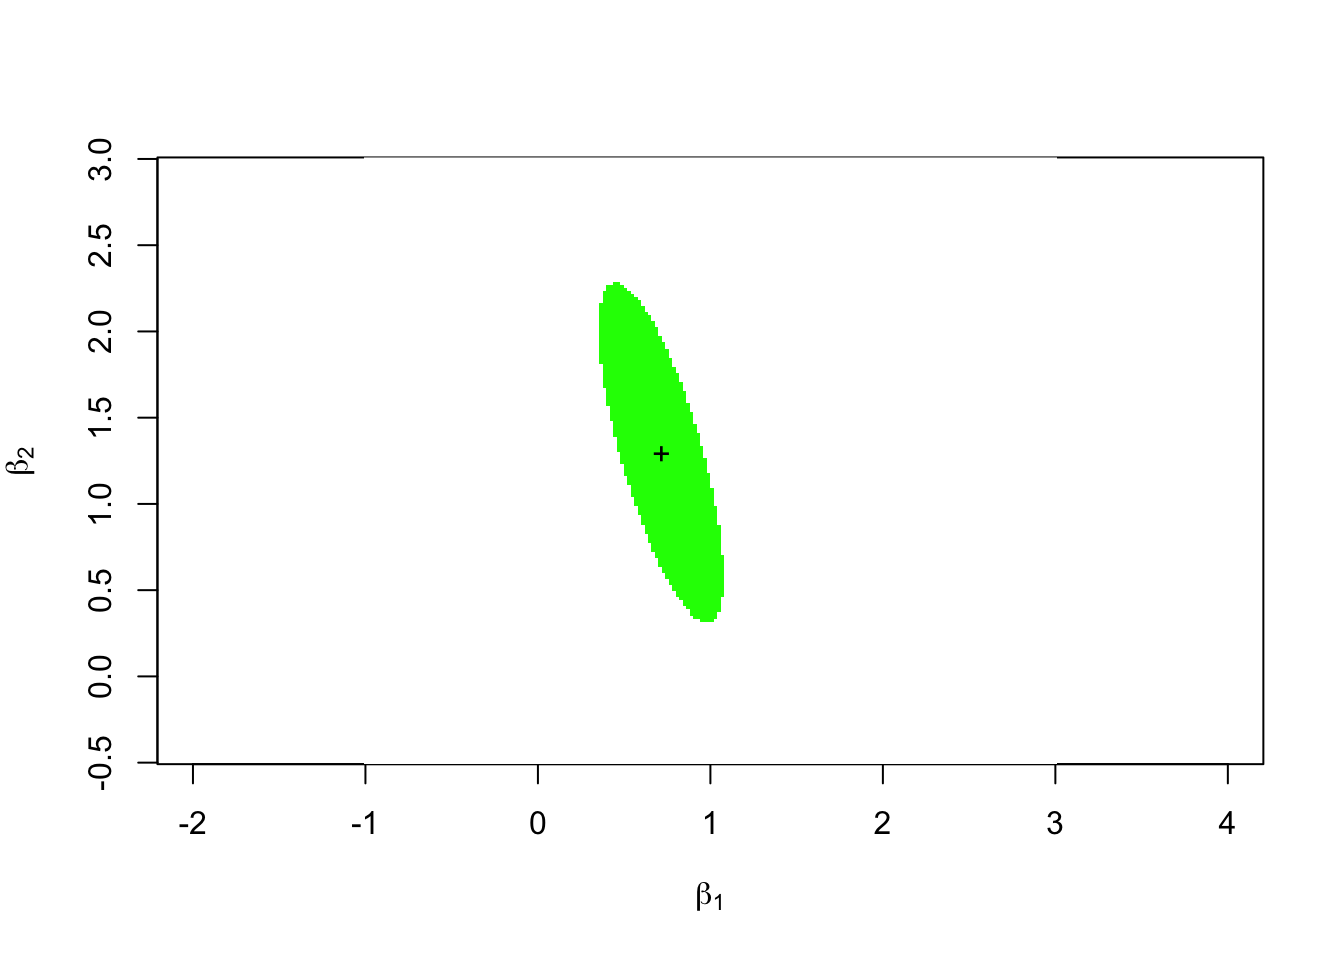
\includegraphics{MATH3714_files/figure-latex/ellipse-1.pdf}

The green ellipse in this plot is the 95\% confidence ellipse
for the vector \((\beta_1, \beta_2)\).

\hypertarget{coordinates-of-the-outline}{%
\paragraph{Coordinates of the Outline}\label{coordinates-of-the-outline}}

\textbf{This sub-section is non-examinable (but hopefully interesting).}

Using some more linear algebra, we can find a formula for the coordinates
of the points on the ellipse which forms the boundary of the confidence
region. For this, we use the
\href{https://en.wikipedia.org/wiki/Singular_value_decomposition}{Singular Value Decomposition}
of the matrix \(Q\). This allows to write \(Q\) as
\begin{equation*}
  Q = U D V^\top
\end{equation*}
where \(U\) and \(V\) are orthogonal matrices and \(D\) is a diagonal matrix:

\begin{Shaded}
\begin{Highlighting}[]
\NormalTok{svd }\OtherTok{\textless{}{-}} \FunctionTok{La.svd}\NormalTok{(Q)}
\NormalTok{svd}
\end{Highlighting}
\end{Shaded}

\begin{Shaded}
\begin{Highlighting}[]
\NormalTok{\# $d}
\NormalTok{\# [1] 0.0138678012 0.0007364967}
\NormalTok{\# }
\NormalTok{\# $u}
\NormalTok{\#            [,1]      [,2]}
\NormalTok{\# [1,] {-}0.2749061 0.9614711}
\NormalTok{\# [2,]  0.9614711 0.2749061}
\NormalTok{\# }
\NormalTok{\# $vt}
\NormalTok{\#            [,1]      [,2]}
\NormalTok{\# [1,] {-}0.2749061 0.9614711}
\NormalTok{\# [2,]  0.9614711 0.2749061}
\end{Highlighting}
\end{Shaded}

The R output shows the diagonal elements \(d_{ii}\) of \(D\) and the matrices \(U\)
and \(V^\top\). Since \(Q\) is symmetric, we have \(U = V\) and thus \(Q = U D U^\top\)
in this case, \(i.e.\)~we have found a diagonalisation of~\(Q\).

Using the SVD we can simplify the norm used in the
definition of the ellipse. We write \(D^{-1/2}\) for the matrix
which has \(1/\sqrt{d_{ii}}\) on the diagonal. Then we have
\begin{align*}
  Q \bigl(D^{-1/2} U^\top \bigr)^\top \bigl(D^{-1/2} U^\top \bigr)
  &= Q U D^{-1/2} D^{-1/2} U^\top \\
  &= U D U^\top U D^{-1} U^\top \\
  &= U D D^{-1} U^\top \\
  &= U U^\top \\
  &= I.
\end{align*}
Thus, \(\bigl(D^{-1/2} U^\top\bigr)^\top \bigl(D^{-1/2} U^\top\bigr)\) is
the inverse of \(Q\) and we get
\begin{align*}
  \bigl\| z - K \hat\beta \bigr\|_Q^2
  &= (z - K \hat\beta)^\top Q^{-1} (z - K \hat\beta) \\
  &= (z - K \hat\beta)^\top \bigl(D^{-1/2} U^\top\bigr)^\top \bigl(D^{-1/2} U^\top\bigr) (z - K \hat\beta) \\
  &= \Bigl\| D^{-1/2} U^\top (z - K \hat\beta) \Bigr\|^2,
\end{align*}
where the norm on the right-hand side is the usual Euclidean norm.
Thus, the boundary of the ellipse consists of all points of the
form \(K \hat\beta + d\), where \(e := D^{-1/2} U^\top d\) is a vector
of length
\[ \| e \| = \sqrt{k \hat\sigma^2 f_{k,n-p-1}(\alpha)}. \]
Finally, using polar coordinates, we find the points on the boundary
to be
\begin{equation*}
  d
  = U D^{1/2} e
  = U D^{1/2} \sqrt{k \hat\sigma^2 f_{k,n-p-1}(\alpha)}
    \begin{pmatrix}
      \cos(\varphi) \\ \sin(\varphi)
    \end{pmatrix}
\end{equation*}
with \(\varphi\in [0, 2\pi]\). This allows to plot the boundary line in~R.

\begin{Shaded}
\begin{Highlighting}[]
\NormalTok{phi }\OtherTok{\textless{}{-}} \FunctionTok{seq}\NormalTok{(}\DecValTok{0}\NormalTok{, }\DecValTok{2}\SpecialCharTok{*}\NormalTok{pi, }\AttributeTok{length.out =} \DecValTok{201}\NormalTok{)}
\NormalTok{circ }\OtherTok{\textless{}{-}} \FunctionTok{rbind}\NormalTok{(}\FunctionTok{cos}\NormalTok{(phi), }\FunctionTok{sin}\NormalTok{(phi)) }\SpecialCharTok{*} \FunctionTok{sqrt}\NormalTok{(f.crit }\SpecialCharTok{*}\NormalTok{ k }\SpecialCharTok{*}\NormalTok{ sigma.hat}\SpecialCharTok{\^{}}\DecValTok{2}\NormalTok{)}

\NormalTok{ellipse }\OtherTok{\textless{}{-}}\NormalTok{ svd}\SpecialCharTok{$}\NormalTok{u }\SpecialCharTok{\%*\%}\NormalTok{ (circ }\SpecialCharTok{*} \FunctionTok{sqrt}\NormalTok{(svd}\SpecialCharTok{$}\NormalTok{d)) }\SpecialCharTok{+}\NormalTok{ K.beta.hat}

\FunctionTok{image}\NormalTok{(}\AttributeTok{x =}\NormalTok{ xx, }\AttributeTok{y =}\NormalTok{ yy, }\FunctionTok{t}\NormalTok{(F }\SpecialCharTok{\textgreater{}}\NormalTok{ f.crit), }\AttributeTok{asp =} \DecValTok{1}\NormalTok{,}
      \AttributeTok{col =} \FunctionTok{c}\NormalTok{(}\StringTok{"green"}\NormalTok{, }\StringTok{"white"}\NormalTok{),}
      \AttributeTok{xlab =} \FunctionTok{expression}\NormalTok{(beta[}\DecValTok{1}\NormalTok{]), }\AttributeTok{ylab =} \FunctionTok{expression}\NormalTok{(beta[}\DecValTok{2}\NormalTok{]))}
\FunctionTok{lines}\NormalTok{(ellipse[}\DecValTok{1}\NormalTok{,], ellipse[}\DecValTok{2}\NormalTok{,])}
\end{Highlighting}
\end{Shaded}

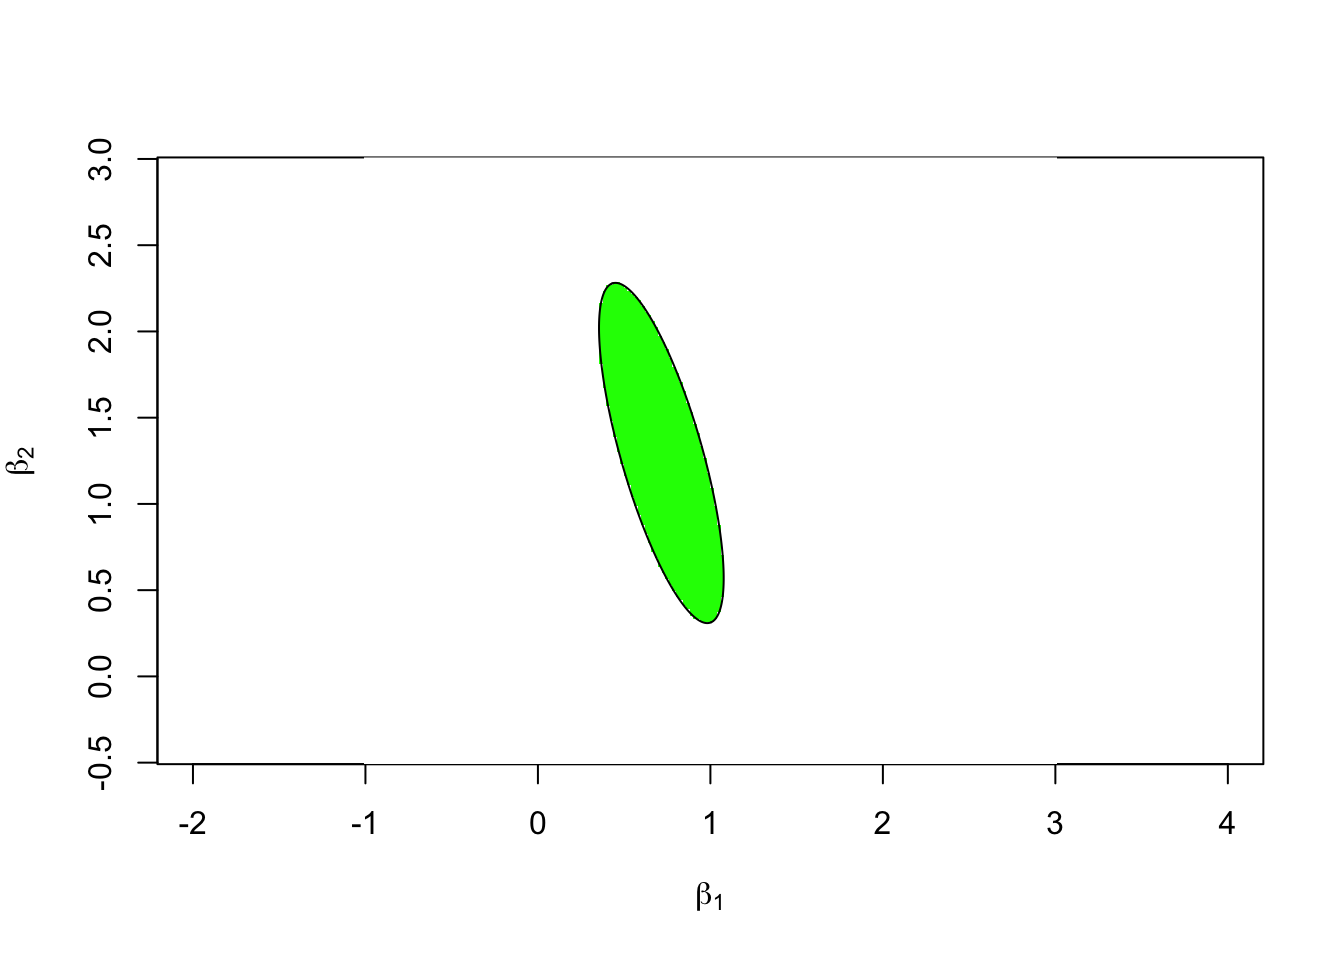
\includegraphics{MATH3714_files/figure-latex/ellipse2-1.pdf}

To verify that everything is consistent, we have plotted the line on top
of the image from the previous subsection. Since the black line perfectly
surrounds the green area, both approaches are consistent.

\hypertarget{sec:simult-test}{%
\subsection{Hypothesis Tests}\label{sec:simult-test}}

We can easily derive a hypothesis test to test the hypothesis
\begin{equation*}
  H_0\colon K\beta = m
\end{equation*}
against the alternative
\begin{equation*}
  H_1\colon K\beta \neq m,
\end{equation*}
where \(m \in \mathbb{R}^k\).

We redefine \(F\) as
\begin{equation*}
  F
  := \frac{\bigl\| K \hat\beta - m \bigr\|_{K(X^\top X)^{-1} K^\top}^2}
          {k \hat\sigma^2}
\end{equation*}
using \(m\) in place of the \(K\beta\) above. Then the new defintion of \(F\)
is the same as~\eqref{eq:simult-F} if \(H_0\) is true.

\begin{lemma}
\protect\hypertarget{lem:simult-test}{}\label{lem:simult-test}The test which rejects \(H_0\) if and only if \(|F| > f_{k,n-p-1}(\alpha)\)
has significance level~\(\alpha\).
\end{lemma}

\begin{proof}
Assume that \(H_0\) is true. Then we have \(K\beta = m\) and thus
the \(F\) defined in this section coincides with the expression from
equation~\eqref{eq:simult-F}. From lemma~\ref{lem:F-dist}
we know that \(F \sim F_{k, n-p-1}\). Thus we have
\begin{align*}
  P( \mbox{type I error} )
  &= P\bigl( F > f_{k,n-p-1}(\alpha) \bigr) \\
  &= 1 - P\bigl( F \leq f_{k,n-p-1}(\alpha) \bigr) \\
  &= 1 - (1 - \alpha) \\
  &= \alpha.
\end{align*}
This completes the proof.
\end{proof}

\clearpage

\hypertarget{I02-read.csv}{%
\section*{Interlude: Loading Data into R}\label{I02-read.csv}}
\addcontentsline{toc}{section}{Interlude: Loading Data into R}

Before we can analyse data using R, we have to ``import'' the data
into~R. How exactly this is done depends on how the data is stored,
and more specifically on which file format is used. Here we consider
two commonly used formats: comma-separated values (\texttt{.csv})
and Microsoft Excel files (\texttt{.xls} or \texttt{.xlsx}).

\hypertarget{importing-csv-files}{%
\subsection*{Importing CSV Files}\label{importing-csv-files}}
\addcontentsline{toc}{subsection}{Importing CSV Files}

The \texttt{read.csv()} command can be used to import \texttt{.csv} files
into R: if we use the command

\begin{Shaded}
\begin{Highlighting}[]
\NormalTok{  x }\OtherTok{\textless{}{-}} \FunctionTok{read.csv}\NormalTok{(}\StringTok{"file.csv"}\NormalTok{)}
\end{Highlighting}
\end{Shaded}

then the contents of the file \texttt{file.csv} will be stored in the variable~\texttt{x}.
Optional arguments to \texttt{read.csv()} can be used to specify whether or not the
file includes column names, and allow to deal with variations of how the data
may be stored in the file. Some of these are explained below.

The most important things to
know about the function \texttt{read.csv()} are:

\begin{itemize}
\item
  The filename can either denote a file on the local computer, or
  a file available for download from the internet. If you want R to read the
  file directly from the internet, replace the file name with the web address
  (starting with \texttt{http://} or~\texttt{https://}).
\item
  If the input file is on the local computer, you may
  need to change R's current directory to the directory where the file is
  stored before calling \texttt{read.csv()}. In RStudio you can use the menu
  ``Session \textgreater{} Set Working Directory \textgreater{} Choose Directory \ldots{}'' to do this. If you
  are not sure what the filename for a given input file is, you can use the
  command \texttt{file.choose()} in place of the file name, to choose a file
  interactively.
\item
  By default, R uses the first row of the \texttt{.csv} file to set
  the column names of the data frame and assumes that the actual data
  starts in row~2 of the \texttt{.csv} file. If the file does not
  contain column names, you can use the \texttt{header=FALSE} option
  with \texttt{read.csv()} to tell R that the column names are not
  included in the data:

\begin{Shaded}
\begin{Highlighting}[]
\NormalTok{  x }\OtherTok{\textless{}{-}} \FunctionTok{read.csv}\NormalTok{(}\StringTok{"file.csv"}\NormalTok{, }\AttributeTok{header=}\ConstantTok{FALSE}\NormalTok{)}
\end{Highlighting}
\end{Shaded}

  You can see whether this option is needed by opening the file in
  Excel and looking whether the first row contains headers or not.
  Alternatively you can inspect the column names and the contents of
  the first data row in R to see whether everything looks right after
  importing the data.
\item
  R uses a special data type called \texttt{Factor} to represent categorical
  data. If the \texttt{.csv} file contains such data, the option
  \texttt{stringsAsFactors=TRUE} can be used to automatically convert
  text to factors. (This option used to be the default for R versions
  before 4.0.0.)
\item
  Sometimes, the columns in a \texttt{.csv} file are separated not
  by a comma, but using a semicolon instead. In this case you
  need to use the option \texttt{sep=";"} when you import the data:

\begin{Shaded}
\begin{Highlighting}[]
\NormalTok{  x }\OtherTok{\textless{}{-}} \FunctionTok{read.csv}\NormalTok{(}\StringTok{"file.csv"}\NormalTok{, }\AttributeTok{sep=}\StringTok{";"}\NormalTok{)}
\end{Highlighting}
\end{Shaded}
\item
  Missing values should be represented by empty cells in the \texttt{.csv}
  file and are represented as special \texttt{NA} values in the data frame.
  If the \texttt{.csv} file uses a different encoding for missing values,
  the \texttt{na.strings} option can be used to tell \texttt{read.csv()}
  which cell values should be interpreted as missing values. For example,
  \texttt{read.csv("file.csv",\ na.strings=c("",\ "-"))} can be used for a file
  where missing values are indicated by either empty cells or cells
  containing a hyphen.
\end{itemize}

Further details about the function \texttt{read.csv()} can be found using the
\href{https://rdrr.io/r/utils/read.table.html}{command \texttt{help(read.csv)}} in~R.

\begin{example}
\protect\hypertarget{exm:l1-poll-import}{}\label{exm:l1-poll-import}In the 2016 version of the MATH1712 module, I performed a small questionnaire
in the first lecture. The following R~command can be used to load the data
from the questionnaire into R

\begin{Shaded}
\begin{Highlighting}[]
\NormalTok{  x }\OtherTok{\textless{}{-}} \FunctionTok{read.csv}\NormalTok{(}\StringTok{"http://www1.maths.leeds.ac.uk/\textasciitilde{}voss/rintro/Q2016.csv"}\NormalTok{)}
\end{Highlighting}
\end{Shaded}

The variable \texttt{x} now contains the questionnaire results.
Instead of
directly downloading the data from the internet into R, you can
alternatively first download the data using a web browser, and then
import the data directly from your computer:

\begin{Shaded}
\begin{Highlighting}[]
\NormalTok{  x }\OtherTok{\textless{}{-}} \FunctionTok{read.csv}\NormalTok{(}\StringTok{"Q2016.csv"}\NormalTok{)}
\end{Highlighting}
\end{Shaded}

Both approaches give the same result.
\end{example}

\hypertarget{importing-microsoft-excel-files}{%
\subsection*{Importing Microsoft Excel Files}\label{importing-microsoft-excel-files}}
\addcontentsline{toc}{subsection}{Importing Microsoft Excel Files}

The easiest way to import Excel files into R is to first convert these
files to \texttt{.csv} format. To do this:

\begin{itemize}
\item
  Open the file with the data in Excel.
\item
  Open a new, empty file (choosing ``Blank workbook'' in Excel).
\item
  Copy and paste the relevant cells into the empty file. It is
  important to just copy the required data and to leave out any
  explanatory text and and empty rows/columns. The data must form a
  tidy rectangle, with one sample per row and one variate per
  column. Optionally, you can put column headers into the first row.
\item
  Save the new file in \texttt{.csv} format
  in a folder where you will find it again.
\item
  Read the resulting \texttt{.csv} into R as explained above.
\end{itemize}

Alternatively, you can try the \texttt{read\_excel()} function from the \texttt{readxl}
package. (You may need to install this R package first.) You can learn how to
use this function at
\url{https://readxl.tidyverse.org/} or using the
\href{https://rdrr.io/cran/readxl/man/read_excel.html}{command \texttt{help(read\_excel)}}.
Note that these functions return a \href{https://tibble.tidyverse.org/}{``tibble''}
instead of a data frame, so some additional knowledge is required to use the
result.

\hypertarget{checking-the-imported-data}{%
\subsection*{Checking the Imported Data}\label{checking-the-imported-data}}
\addcontentsline{toc}{subsection}{Checking the Imported Data}

The following commands can be used to get a quick overview over the data:

\begin{itemize}
\item
  \texttt{dim(x)} gives the number of rows and columns of the data
  frame. Similarly, \texttt{nrow(x)} shows the number of rows
  and \texttt{ncol(x)} shows the number of columns in the data frame.
\item
  \texttt{str(x)} shows the structure of any R object. This command
  is often an excellent way to understand the nature of any problems
  one may encounter while importing data into~R.
\item
  \texttt{summary(x)} prints, for each variate, the values of
  various summary statistics. For variates with numeric values,
  these are the minimum, first quartile, median, mean, third quartile,
  maximum, and the number of missing values. For attribute data
  this gives the counts for each observed value.
\item
  \texttt{head(x)} shows the first few rows of the data.
\end{itemize}

Every time you import a dataset into R, you should use some
of these commands to check that everything went well.
In case you discover problems, you should either fix the data file
(\emph{e.g.}~using Microsoft Excel) or by using the correct options
for the \texttt{read.csv()} command.

\begin{example}
Continuing with the dataset from example above, we can try the following
commands: We first check that the data has plausible dimensions:

\begin{Shaded}
\begin{Highlighting}[]
\FunctionTok{dim}\NormalTok{(x)}
\end{Highlighting}
\end{Shaded}

\begin{Shaded}
\begin{Highlighting}[]
\NormalTok{\# [1] 220   5}
\end{Highlighting}
\end{Shaded}

This tells us that the data has \(n=220\) rows and \(p=5\) columns, as expected.
Next, we get some details about the five columns of the data frame:

\begin{Shaded}
\begin{Highlighting}[]
\FunctionTok{str}\NormalTok{(x)}
\end{Highlighting}
\end{Shaded}

\begin{Shaded}
\begin{Highlighting}[]
\NormalTok{\# \textquotesingle{}data.frame\textquotesingle{}: 220 obs. of  5 variables:}
\NormalTok{\#  $ gender     : chr  "M" "M" "M" "M" ...}
\NormalTok{\#  $ height     : num  180 183 183 182 164 ...}
\NormalTok{\#  $ handedness : chr  "R" "R" "R" "R" ...}
\NormalTok{\#  $ travel.time: int  20 25 20 12 5 20 15 10 11 7 ...}
\NormalTok{\#  $ R.skills   : chr  "basic" "basic" "basic" "basic" ...}
\end{Highlighting}
\end{Shaded}

This shows, for each column, the name, the ``data type'' and the
first few values. The ``data type'' is a good indicator to detect
problems; it should read \texttt{int} for integer valued numeric data,
\texttt{num} for all other numeric data, and \texttt{Factor} for
attribute data. For attribute data, the range of observed values is
also shown. For our dataset, we see that the fields \texttt{\$gender},
\texttt{\$handedness} and \texttt{\$R.skills} are represented as text data (type \texttt{chr})
instead of categorical data. To fix this, we re-import the data
using the \texttt{stringsAsFactors=TRUE} option:

\begin{Shaded}
\begin{Highlighting}[]
\NormalTok{x }\OtherTok{\textless{}{-}} \FunctionTok{read.csv}\NormalTok{(}\StringTok{"data/Q2016.csv"}\NormalTok{, }\AttributeTok{stringsAsFactors=}\ConstantTok{TRUE}\NormalTok{)}
\FunctionTok{str}\NormalTok{(x)}
\end{Highlighting}
\end{Shaded}

\begin{Shaded}
\begin{Highlighting}[]
\NormalTok{\# \textquotesingle{}data.frame\textquotesingle{}: 220 obs. of  5 variables:}
\NormalTok{\#  $ gender     : Factor w/ 2 levels "F","M": 2 2 2 2 1 1 1 1 1 2 ...}
\NormalTok{\#  $ height     : num  180 183 183 182 164 ...}
\NormalTok{\#  $ handedness : Factor w/ 3 levels "L","R","both": 2 2 2 2 2 2 2 2 2 2 ...}
\NormalTok{\#  $ travel.time: int  20 25 20 12 5 20 15 10 11 7 ...}
\NormalTok{\#  $ R.skills   : Factor w/ 4 levels "basic","good",..: 1 1 1 1 1 1 1 3 1 1 ...}
\end{Highlighting}
\end{Shaded}

Now the output is as expected, and the correct ``levels'' are shown
for the categorical variables.

Finally, we can print summary statistics for all columns:

\begin{Shaded}
\begin{Highlighting}[]
\FunctionTok{summary}\NormalTok{(x)}
\end{Highlighting}
\end{Shaded}

\begin{Shaded}
\begin{Highlighting}[]
\NormalTok{\#  gender      height      handedness  travel.time       R.skills  }
\NormalTok{\#  F:102   Min.   :147.0   L   : 18   Min.   :  0.00   basic :157  }
\NormalTok{\#  M:118   1st Qu.:167.0   R   :201   1st Qu.:  5.00   good  :  4  }
\NormalTok{\#          Median :175.0   both:  1   Median : 15.00   medium: 28  }
\NormalTok{\#          Mean   :173.7              Mean   : 19.15   none  : 31  }
\NormalTok{\#          3rd Qu.:180.3              3rd Qu.: 25.00               }
\NormalTok{\#          Max.   :195.6              Max.   :150.00               }
\NormalTok{\#          NA\textquotesingle{}s   :23}
\end{Highlighting}
\end{Shaded}

None of these commands showed any remaining problems, so we are now ready
to use the data.
\end{example}

\hypertarget{common-problems}{%
\subsection*{Common Problems}\label{common-problems}}
\addcontentsline{toc}{subsection}{Common Problems}

There are many things which can go wrong when importing data. Some commonly
encountered problems are the following:

\begin{itemize}
\item
  If the data file contains no line with headers, but the
  \texttt{header=FALSE} option for \texttt{read.csv()} has been omitted,
  the first row of data will be used in place of the column names.
  This can, for example, be seen in the \texttt{str()} output. The
  solution to this problem is to correctly use the
  \texttt{header=FALSE} option.
\item
  If the data in a \texttt{.csv} file is not separated by commas but
  by some other character like a semicolon, R will be unable to
  separate the columns. When this is the case, the imported data will
  appear to only have one column, where each entry shows as some
  garbled version of the data for the whole row. The solution to this
  problem is to use the \texttt{sep=...} option.
\item
  If attribute values are encoded inconsistently, \emph{e.g.}~if
  a mix of \texttt{m} and \texttt{M} is used to encode the gender
  ``male'', this will be visible in the \texttt{str()} output. One
  solution to this problem is to fix the \texttt{.csv} file using
  Microsoft Excel, before trying to import it into R again.
\item
  If a numeric column in the input file contains one or more
  entries which are neither numbers nor empty, R will interpret the
  whole column as attribute data. This problem can be detected in the
  \texttt{str()} output, when a numeric column is listed as having data
  type \texttt{Factor}. One solution to this problem is to use
  Microsoft Excel to remove or fix the offending entry from the file.
\end{itemize}

\clearpage

\hypertarget{S07-examples}{%
\section{Examples}\label{S07-examples}}

To illustrate the results of the last two sections, we consider a series
of examples.

\hypertarget{simple-confidence-interval}{%
\subsection{Simple Confidence Interval}\label{simple-confidence-interval}}

In this subsection we will illustrate how to compute a simple confidence interval
for a single regression coefficient. We use a dataset about toxicity of
chemicals towards aquatic life from the from the UCI Machine Learning
Repository. The data is available at

\begin{itemize}
\tightlist
\item
  \url{https://archive.ics.uci.edu/ml/datasets/QSAR+aquatic+toxicity}
\end{itemize}

There are nine different variables. (The web page explains the interpretation
of these variables.) We will fit a model which describes \texttt{LC50} as a function
of the remaining variables:

\begin{Shaded}
\begin{Highlighting}[]
\CommentTok{\# data from https://archive.ics.uci.edu/ml/datasets/QSAR+aquatic+toxicity}
\NormalTok{qsar }\OtherTok{\textless{}{-}} \FunctionTok{read.csv}\NormalTok{(}\StringTok{"data/qsar\_aquatic\_toxicity.csv"}\NormalTok{, }\AttributeTok{sep =} \StringTok{";"}\NormalTok{, }\AttributeTok{header =} \ConstantTok{FALSE}\NormalTok{)}
\FunctionTok{names}\NormalTok{(qsar) }\OtherTok{\textless{}{-}} \FunctionTok{c}\NormalTok{(}
    \StringTok{"TPSA"}\NormalTok{,}
    \StringTok{"SAacc"}\NormalTok{,}
    \StringTok{"H050"}\NormalTok{,}
    \StringTok{"MLOGP"}\NormalTok{,}
    \StringTok{"RDCHI"}\NormalTok{,}
    \StringTok{"GATS1p"}\NormalTok{,}
    \StringTok{"nN"}\NormalTok{,}
    \StringTok{"C040"}\NormalTok{,}
    \StringTok{"LC50"}
\NormalTok{)}
\NormalTok{m }\OtherTok{\textless{}{-}} \FunctionTok{lm}\NormalTok{(LC50 }\SpecialCharTok{\textasciitilde{}}\NormalTok{ ., }\AttributeTok{data =}\NormalTok{ qsar)}
\FunctionTok{summary}\NormalTok{(m)}
\end{Highlighting}
\end{Shaded}

\begin{Shaded}
\begin{Highlighting}[]
\NormalTok{\# }
\NormalTok{\# Call:}
\NormalTok{\# lm(formula = LC50 \textasciitilde{} ., data = qsar)}
\NormalTok{\# }
\NormalTok{\# Residuals:}
\NormalTok{\#     Min      1Q  Median      3Q     Max }
\NormalTok{\# {-}4.4934 {-}0.7579 {-}0.1120  0.5829  4.9778 }
\NormalTok{\# }
\NormalTok{\# Coefficients:}
\NormalTok{\#              Estimate Std. Error t value Pr(\textgreater{}|t|)    }
\NormalTok{\# (Intercept)  2.698887   0.244554  11.036  \textless{} 2e{-}16 ***}
\NormalTok{\# TPSA         0.027201   0.002661  10.220  \textless{} 2e{-}16 ***}
\NormalTok{\# SAacc       {-}0.015081   0.002091  {-}7.211 1.90e{-}12 ***}
\NormalTok{\# H050         0.040619   0.059787   0.679 0.497186    }
\NormalTok{\# MLOGP        0.446108   0.063296   7.048 5.60e{-}12 ***}
\NormalTok{\# RDCHI        0.513928   0.135565   3.791 0.000167 ***}
\NormalTok{\# GATS1p      {-}0.571313   0.153882  {-}3.713 0.000227 ***}
\NormalTok{\# nN          {-}0.224751   0.048301  {-}4.653 4.12e{-}06 ***}
\NormalTok{\# C040         0.003194   0.077972   0.041 0.967340    }
\NormalTok{\# {-}{-}{-}}
\NormalTok{\# Signif. codes:  0 \textquotesingle{}***\textquotesingle{} 0.001 \textquotesingle{}**\textquotesingle{} 0.01 \textquotesingle{}*\textquotesingle{} 0.05 \textquotesingle{}.\textquotesingle{} 0.1 \textquotesingle{} \textquotesingle{} 1}
\NormalTok{\# }
\NormalTok{\# Residual standard error: 1.203 on 537 degrees of freedom}
\NormalTok{\# Multiple R{-}squared:  0.4861,  Adjusted R{-}squared:  0.4785 }
\NormalTok{\# F{-}statistic:  63.5 on 8 and 537 DF,  p{-}value: \textless{} 2.2e{-}16}
\end{Highlighting}
\end{Shaded}

Our aim is to find a 95\% confidence interval for \texttt{GATS1p}.

\hypertarget{from-first-principles}{%
\subsubsection{From First Principles}\label{from-first-principles}}

To compute the confidence interval from first principles,
we can use Lemma~\ref{lem:single-CI}. The centre of the confidence
interval is given by \(\hat\beta_i\):

\begin{Shaded}
\begin{Highlighting}[]
\NormalTok{mid }\OtherTok{\textless{}{-}} \FunctionTok{coef}\NormalTok{(m)[}\DecValTok{7}\NormalTok{]}
\NormalTok{mid}
\end{Highlighting}
\end{Shaded}

\begin{Shaded}
\begin{Highlighting}[]
\NormalTok{\#     GATS1p }
\NormalTok{\# {-}0.5713131}
\end{Highlighting}
\end{Shaded}

To find the half-width of the interval, we need to first construct the
covariance matrix \(C\) and the estimated residual variance \(\hat\sigma^2\).
We will also need the corresponding quantile of the \(t\)-distribution.

\begin{Shaded}
\begin{Highlighting}[]
\NormalTok{X }\OtherTok{\textless{}{-}} \FunctionTok{model.matrix}\NormalTok{(m)}
\NormalTok{y }\OtherTok{\textless{}{-}}\NormalTok{ qsar}\SpecialCharTok{$}\NormalTok{LC50}
\NormalTok{n }\OtherTok{\textless{}{-}} \FunctionTok{nrow}\NormalTok{(X)}
\NormalTok{p }\OtherTok{\textless{}{-}} \FunctionTok{ncol}\NormalTok{(X) }\SpecialCharTok{{-}} \DecValTok{1}

\NormalTok{Cii }\OtherTok{\textless{}{-}} \FunctionTok{solve}\NormalTok{(}\FunctionTok{t}\NormalTok{(X) }\SpecialCharTok{\%*\%}\NormalTok{ X)[}\DecValTok{7}\NormalTok{, }\DecValTok{7}\NormalTok{]}
\FunctionTok{cat}\NormalTok{(}\StringTok{"Cii ="}\NormalTok{, Cii, }\StringTok{"}\SpecialCharTok{\textbackslash{}n}\StringTok{"}\NormalTok{)}
\end{Highlighting}
\end{Shaded}

\begin{Shaded}
\begin{Highlighting}[]
\NormalTok{\# Cii = 0.01637454}
\end{Highlighting}
\end{Shaded}

\begin{Shaded}
\begin{Highlighting}[]
\NormalTok{sigma.hat.squared }\OtherTok{\textless{}{-}} \FunctionTok{sum}\NormalTok{((}\FunctionTok{fitted}\NormalTok{(m) }\SpecialCharTok{{-}}\NormalTok{ y)}\SpecialCharTok{\^{}}\DecValTok{2}\NormalTok{) }\SpecialCharTok{/}\NormalTok{ (n }\SpecialCharTok{{-}}\NormalTok{ p }\SpecialCharTok{{-}} \DecValTok{1}\NormalTok{)}
\FunctionTok{cat}\NormalTok{(}\StringTok{"hat.sigma.square ="}\NormalTok{, sigma.hat.squared, }\StringTok{"}\SpecialCharTok{\textbackslash{}n}\StringTok{"}\NormalTok{)}
\end{Highlighting}
\end{Shaded}

\begin{Shaded}
\begin{Highlighting}[]
\NormalTok{\# hat.sigma.square = 1.446134}
\end{Highlighting}
\end{Shaded}

\begin{Shaded}
\begin{Highlighting}[]
\NormalTok{alpha }\OtherTok{\textless{}{-}} \FloatTok{0.05}
\NormalTok{t }\OtherTok{\textless{}{-}} \FunctionTok{qt}\NormalTok{(}\DecValTok{1} \SpecialCharTok{{-}}\NormalTok{ alpha}\SpecialCharTok{/}\DecValTok{2}\NormalTok{, n }\SpecialCharTok{{-}}\NormalTok{ p }\SpecialCharTok{{-}} \DecValTok{1}\NormalTok{)}
\FunctionTok{cat}\NormalTok{(}\StringTok{"t ="}\NormalTok{, t, }\StringTok{"}\SpecialCharTok{\textbackslash{}n}\StringTok{"}\NormalTok{)}
\end{Highlighting}
\end{Shaded}

\begin{Shaded}
\begin{Highlighting}[]
\NormalTok{\# t = 1.964391}
\end{Highlighting}
\end{Shaded}

With this information in place, we can easily find the confidence
interval:

\begin{Shaded}
\begin{Highlighting}[]
\NormalTok{d }\OtherTok{\textless{}{-}} \FunctionTok{sqrt}\NormalTok{(Cii }\SpecialCharTok{*}\NormalTok{ sigma.hat.squared) }\SpecialCharTok{*}\NormalTok{ t}
\FunctionTok{cat}\NormalTok{(}\StringTok{"["}\NormalTok{, mid }\SpecialCharTok{{-}}\NormalTok{ d, }\StringTok{", "}\NormalTok{, mid }\SpecialCharTok{+}\NormalTok{ d, }\StringTok{"]}\SpecialCharTok{\textbackslash{}n}\StringTok{"}\NormalTok{, }\AttributeTok{sep =} \StringTok{""}\NormalTok{)}
\end{Highlighting}
\end{Shaded}

\begin{Shaded}
\begin{Highlighting}[]
\NormalTok{\# [{-}0.8735983, {-}0.2690279]}
\end{Highlighting}
\end{Shaded}

\hypertarget{from-the-lm-output}{%
\subsubsection{\texorpdfstring{From the \texttt{lm()} Output}{From the lm() Output}}\label{from-the-lm-output}}

We can obtain the same result using only the quantile \(t\) and
numbers shows in the \texttt{summary(m)} output. We focus on the
row corresponding to \texttt{GATS1p} in the output shown above:

\begin{verbatim}
GATS1p      -0.571313   0.153882  -3.713 0.000227 ***
\end{verbatim}

The first number in this row is the centre of the confidence
interval, the second number corresponds to \(\sqrt{\hat\sigma^2 C_{ii}}\).
To have everything in one place, we copy the commands for computing~\(t\):

\begin{Shaded}
\begin{Highlighting}[]
\NormalTok{alpha }\OtherTok{\textless{}{-}} \FloatTok{0.05}
\NormalTok{t }\OtherTok{\textless{}{-}} \FunctionTok{qt}\NormalTok{(}\DecValTok{1} \SpecialCharTok{{-}}\NormalTok{ alpha}\SpecialCharTok{/}\DecValTok{2}\NormalTok{, n }\SpecialCharTok{{-}}\NormalTok{ p }\SpecialCharTok{{-}} \DecValTok{1}\NormalTok{)}
\FunctionTok{cat}\NormalTok{(}\StringTok{"["}\NormalTok{, }\SpecialCharTok{{-}}\FloatTok{0.571313} \SpecialCharTok{{-}} \FloatTok{0.153882}\SpecialCharTok{*}\NormalTok{t, }\StringTok{", "}\NormalTok{, }\SpecialCharTok{{-}}\FloatTok{0.571313} \SpecialCharTok{+} \FloatTok{0.153882}\SpecialCharTok{*}\NormalTok{t, }\StringTok{"]}\SpecialCharTok{\textbackslash{}n}\StringTok{"}\NormalTok{, }\AttributeTok{sep =} \StringTok{""}\NormalTok{)}
\end{Highlighting}
\end{Shaded}

\begin{Shaded}
\begin{Highlighting}[]
\NormalTok{\# [{-}0.8735975, {-}0.2690285]}
\end{Highlighting}
\end{Shaded}

This is the same result as above.

\hypertarget{confidence-intervals-for-the-mean}{%
\subsection{Confidence Intervals for the Mean}\label{confidence-intervals-for-the-mean}}

So far we have only seen how to compute confidence intervals for the
regression coefficients \(\beta_i\). Using the same techniques we can
also compute confidence intervals for the model mean corresponding
to an input \((\tilde x_1, \ldots, \tilde x_p)\). If we write
\begin{equation*}
  \tilde x = (1, \tilde x_1, \ldots, \tilde x_p),
\end{equation*}
then the model mean corresponding to this input is
\begin{equation*}
  \tilde y
  = \beta_0 + \tilde x_1 \beta_1 + \cdots + \tilde x_p \beta_p
  = \tilde x^\top \beta,
\end{equation*}
To derive a confidence interval for this quantity, we follow the same
steps as we did when we derived a confidence interval for \(\hat\beta_i\).

Our estimator for this \(\tilde y\) is
\begin{equation*}
  \hat y
  = \tilde x^\top \hat\beta
  \sim \mathcal{N}\bigl( \tilde x^\top \beta, \sigma^2 \tilde x^\top (X^\top X)^{-1} \tilde x \bigr).
\end{equation*}
Thus,
\begin{align*}
  \tilde T
  &:= \frac{\tilde x^\top \hat\beta - \tilde x^\top \beta}
           {\sqrt{\hat\sigma^2 \tilde x^\top (X^\top X)^{-1} \tilde x}} \\
  &= \frac{\frac{1}{\sqrt{\sigma^2\tilde x^\top (X^\top X)^{-1} \tilde x}}\bigl(\tilde x^\top \hat\beta - \tilde x^\top \beta\bigr)}
           {\sqrt{\frac{1}{\sigma^2}\hat\sigma^2}}
\end{align*}
is \(t(n-p-1)\)-distributed, since the numerator is \(\mathcal{N}(0,1)\), the denominator
is \(\sqrt{\chi^2(n-p-1) / (n-p-1)}\) and \(\hat\beta\) is independent
of~\(\hat\sigma^2\).
Let \(t_{n-p-1}(\alpha/2)\) be the \((1 - \alpha/2)\)-quantile of the \(t(n-p-1)\)-distribution.
Then we can solve the inequality \(|T| \leq t_{n-p-1}(\alpha/2)\) for
\(\tilde x^\top \beta\) to find the required confidence interval:
\begin{equation*}
  \Bigl[
    \tilde x^\top \hat\beta - \sqrt{\hat\sigma^2 \tilde x^\top (X^\top X)^{-1} \tilde x} t_{n-p-1}(\alpha/2),
    \tilde x^\top \hat\beta + \sqrt{\hat\sigma^2 \tilde x^\top (X^\top X)^{-1} \tilde x} t_{n-p-1}(\alpha/2)
  \Bigr].
\end{equation*}

We illustrate this using a numerical example.
For the \href{https://rdrr.io/r/datasets/stackloss.html}{\texttt{stackloss} dataset}
with input values \texttt{Air.Flow\ =\ 60}, \texttt{Water.Temp\ =\ 21} and \texttt{Acid.Conc\ =\ 87},
we can get the following results:

\begin{Shaded}
\begin{Highlighting}[]
\NormalTok{m }\OtherTok{\textless{}{-}} \FunctionTok{lm}\NormalTok{(stack.loss }\SpecialCharTok{\textasciitilde{}}\NormalTok{ ., }\AttributeTok{data =}\NormalTok{ stackloss)}
\NormalTok{X }\OtherTok{\textless{}{-}} \FunctionTok{model.matrix}\NormalTok{(m)}
\NormalTok{n }\OtherTok{\textless{}{-}} \FunctionTok{nrow}\NormalTok{(X)}
\NormalTok{p }\OtherTok{\textless{}{-}} \FunctionTok{ncol}\NormalTok{(X) }\SpecialCharTok{{-}} \DecValTok{1}

\NormalTok{tilde.x }\OtherTok{\textless{}{-}} \FunctionTok{c}\NormalTok{(}\DecValTok{1}\NormalTok{, }\DecValTok{60}\NormalTok{, }\DecValTok{21}\NormalTok{, }\DecValTok{87}\NormalTok{)}
\NormalTok{hat.beta }\OtherTok{\textless{}{-}} \FunctionTok{coef}\NormalTok{(m)}

\NormalTok{c }\OtherTok{\textless{}{-}} \FunctionTok{t}\NormalTok{(tilde.x) }\SpecialCharTok{\%*\%} \FunctionTok{solve}\NormalTok{(}\FunctionTok{t}\NormalTok{(X) }\SpecialCharTok{\%*\%}\NormalTok{ X, tilde.x)}
\NormalTok{sigma.hat.squared }\OtherTok{\textless{}{-}} \FunctionTok{sum}\NormalTok{((}\FunctionTok{fitted}\NormalTok{(m) }\SpecialCharTok{{-}}\NormalTok{ stackloss}\SpecialCharTok{$}\NormalTok{stack.loss)}\SpecialCharTok{\^{}}\DecValTok{2}\NormalTok{) }\SpecialCharTok{/}\NormalTok{ (n }\SpecialCharTok{{-}}\NormalTok{ p }\SpecialCharTok{{-}} \DecValTok{1}\NormalTok{)}
\NormalTok{t }\OtherTok{\textless{}{-}} \FunctionTok{qt}\NormalTok{(}\FloatTok{0.975}\NormalTok{, n }\SpecialCharTok{{-}}\NormalTok{ p }\SpecialCharTok{{-}} \DecValTok{1}\NormalTok{)}

\NormalTok{mid }\OtherTok{\textless{}{-}} \FunctionTok{t}\NormalTok{(tilde.x) }\SpecialCharTok{\%*\%}\NormalTok{ hat.beta}
\NormalTok{d }\OtherTok{\textless{}{-}} \FunctionTok{sqrt}\NormalTok{(c }\SpecialCharTok{*}\NormalTok{ sigma.hat.squared) }\SpecialCharTok{*}\NormalTok{ t}
\FunctionTok{cat}\NormalTok{(}\StringTok{"["}\NormalTok{, mid }\SpecialCharTok{{-}}\NormalTok{ d, }\StringTok{", "}\NormalTok{, mid }\SpecialCharTok{+}\NormalTok{ d, }\StringTok{"]}\SpecialCharTok{\textbackslash{}n}\StringTok{"}\NormalTok{, }\AttributeTok{sep =} \StringTok{""}\NormalTok{)}
\end{Highlighting}
\end{Shaded}

\begin{Shaded}
\begin{Highlighting}[]
\NormalTok{\# [15.46463, 18.50554]}
\end{Highlighting}
\end{Shaded}

\hypertarget{testing-a-single-coefficient}{%
\subsection{Testing a Single Coefficient}\label{testing-a-single-coefficient}}

Continuing with the dataset from the previous example, we can test whether the
regression coefficient corresponding to the water temperature might equal zero.
We will perform a test at \(5\%\)-level.

\hypertarget{from-first-principles-1}{%
\subsubsection{From First Principles}\label{from-first-principles-1}}

We can compute the test statistic manually, using the formula from
equation~\eqref{eq:single-test} with \(b = 0\):

\begin{Shaded}
\begin{Highlighting}[]
\NormalTok{T }\OtherTok{\textless{}{-}}\NormalTok{ hat.beta[}\DecValTok{3}\NormalTok{] }\SpecialCharTok{/} \FunctionTok{sqrt}\NormalTok{(sigma.hat.squared }\SpecialCharTok{*} \FunctionTok{solve}\NormalTok{(}\FunctionTok{t}\NormalTok{(X) }\SpecialCharTok{\%*\%}\NormalTok{ X)[}\DecValTok{3}\NormalTok{, }\DecValTok{3}\NormalTok{])}
\NormalTok{T}
\end{Highlighting}
\end{Shaded}

\begin{Shaded}
\begin{Highlighting}[]
\NormalTok{\# Water.Temp }
\NormalTok{\#   3.519567}
\end{Highlighting}
\end{Shaded}

\begin{Shaded}
\begin{Highlighting}[]
\NormalTok{t.crit }\OtherTok{\textless{}{-}} \FunctionTok{qt}\NormalTok{(}\FloatTok{0.975}\NormalTok{, n }\SpecialCharTok{{-}}\NormalTok{ p }\SpecialCharTok{{-}} \DecValTok{1}\NormalTok{)}
\FunctionTok{abs}\NormalTok{(T) }\SpecialCharTok{\textgreater{}}\NormalTok{ t.crit}
\end{Highlighting}
\end{Shaded}

\begin{Shaded}
\begin{Highlighting}[]
\NormalTok{\# Water.Temp }
\NormalTok{\#       TRUE}
\end{Highlighting}
\end{Shaded}

Since the test statistic is larger than the critical value,
we reject the hypothesis that \(\beta_2 = 0\).

\hypertarget{using-the-lm-output-i}{%
\subsubsection{\texorpdfstring{Using the \texttt{lm()} Output, I}{Using the lm() Output, I}}\label{using-the-lm-output-i}}

We can also find the test statistic in the \texttt{lm()} output:

\begin{Shaded}
\begin{Highlighting}[]
\FunctionTok{summary}\NormalTok{(m)}
\end{Highlighting}
\end{Shaded}

\begin{Shaded}
\begin{Highlighting}[]
\NormalTok{\# }
\NormalTok{\# Call:}
\NormalTok{\# lm(formula = stack.loss \textasciitilde{} ., data = stackloss)}
\NormalTok{\# }
\NormalTok{\# Residuals:}
\NormalTok{\#     Min      1Q  Median      3Q     Max }
\NormalTok{\# {-}7.2377 {-}1.7117 {-}0.4551  2.3614  5.6978 }
\NormalTok{\# }
\NormalTok{\# Coefficients:}
\NormalTok{\#             Estimate Std. Error t value Pr(\textgreater{}|t|)    }
\NormalTok{\# (Intercept) {-}39.9197    11.8960  {-}3.356  0.00375 ** }
\NormalTok{\# Air.Flow      0.7156     0.1349   5.307  5.8e{-}05 ***}
\NormalTok{\# Water.Temp    1.2953     0.3680   3.520  0.00263 ** }
\NormalTok{\# Acid.Conc.   {-}0.1521     0.1563  {-}0.973  0.34405    }
\NormalTok{\# {-}{-}{-}}
\NormalTok{\# Signif. codes:  0 \textquotesingle{}***\textquotesingle{} 0.001 \textquotesingle{}**\textquotesingle{} 0.01 \textquotesingle{}*\textquotesingle{} 0.05 \textquotesingle{}.\textquotesingle{} 0.1 \textquotesingle{} \textquotesingle{} 1}
\NormalTok{\# }
\NormalTok{\# Residual standard error: 3.243 on 17 degrees of freedom}
\NormalTok{\# Multiple R{-}squared:  0.9136,  Adjusted R{-}squared:  0.8983 }
\NormalTok{\# F{-}statistic:  59.9 on 3 and 17 DF,  p{-}value: 3.016e{-}09}
\end{Highlighting}
\end{Shaded}

The column \texttt{t\ value} shows the value of the test statistic \(T\) for
the hypothesis that \(\beta_i = 0\). For \(\beta_2\) we find the value \(3.520\),
which is a rounded version of the \(3.519567\) we found above.

Again, we can use the command \texttt{qt(0.975,\ 17)} to get the critical value, where
we can find the degrees of freedom in the \texttt{Residual\ standard\ error} row near
the bottom. Alternatively, we can use the so called ``p-value'' listed in the
\texttt{Pr(\textgreater{}\textbar{}t\textbar{})} column. This value is the smallest significance level at which
\(H_0\) is still rejected. Here we find \(0.00263\) and since we have
\(\alpha = 0.05 > 0.00263\), we can see that \(H_0\) is rejected.

If we wanted to test \(\beta_2 = 1\) instead, we could use the value \(\hat\beta_2 = 1.2953\) from the \texttt{Estimate} column and \(\sqrt{\hat\sigma^2 C_{ii}} = 0.3680\)
from the \texttt{Std.\ Error} column, to get \(T = (1.2953 - 1) / 0.3680\) and then we
would accept or reject the hypothesis \(\beta_2 = 1\) by comparing the result to
the critical value~\texttt{qt(0.975,\ 17)}.

\hypertarget{using-the-lm-output-ii}{%
\subsubsection{\texorpdfstring{Using the \texttt{lm()} Output, II}{Using the lm() Output, II}}\label{using-the-lm-output-ii}}

For the hypotheses \(\beta_i = 0\), we can also use the stars (or sometimes dots)
shown in the right margin to perform the test. Since the \texttt{Water.Temp} row ends
in \texttt{**}, we would reject \(\beta_2 = 0\) even at the stricter \(\alpha=0.01\)
level, and thus we would also reject this hypothesis at \(\alpha=0.05\) level.

\hypertarget{testing-multiple-coefficents}{%
\subsection{Testing Multiple Coefficents}\label{testing-multiple-coefficents}}

This section illustrates how a group of coefficients can be tested
simultaneously. We consider a small, synthetic dataset:

\begin{Shaded}
\begin{Highlighting}[]
\CommentTok{\# data from https://www1.maths.leeds.ac.uk/\textasciitilde{}voss/data/small/small.csv}
\NormalTok{small }\OtherTok{\textless{}{-}} \FunctionTok{read.csv}\NormalTok{(}\StringTok{"data/small.csv"}\NormalTok{)}
\NormalTok{m }\OtherTok{\textless{}{-}} \FunctionTok{lm}\NormalTok{(y }\SpecialCharTok{\textasciitilde{}}\NormalTok{ ., }\AttributeTok{data =}\NormalTok{ small)}
\FunctionTok{summary}\NormalTok{(m)}
\end{Highlighting}
\end{Shaded}

\begin{Shaded}
\begin{Highlighting}[]
\NormalTok{\# }
\NormalTok{\# Call:}
\NormalTok{\# lm(formula = y \textasciitilde{} ., data = small)}
\NormalTok{\# }
\NormalTok{\# Residuals:}
\NormalTok{\#      Min       1Q   Median       3Q      Max }
\NormalTok{\# {-}0.64664 {-}0.09369 {-}0.03420  0.07768  0.63353 }
\NormalTok{\# }
\NormalTok{\# Coefficients:}
\NormalTok{\#             Estimate Std. Error t value Pr(\textgreater{}|t|)    }
\NormalTok{\# (Intercept)  5.53329    0.12360  44.768 6.92e{-}12 ***}
\NormalTok{\# x1           0.18903    0.12059   1.568   0.1514    }
\NormalTok{\# x2          {-}0.30731    0.18011  {-}1.706   0.1221    }
\NormalTok{\# x3          {-}0.12382    0.05639  {-}2.196   0.0557 .  }
\NormalTok{\# x4          {-}0.11731    0.12619  {-}0.930   0.3768    }
\NormalTok{\# {-}{-}{-}}
\NormalTok{\# Signif. codes:  0 \textquotesingle{}***\textquotesingle{} 0.001 \textquotesingle{}**\textquotesingle{} 0.01 \textquotesingle{}*\textquotesingle{} 0.05 \textquotesingle{}.\textquotesingle{} 0.1 \textquotesingle{} \textquotesingle{} 1}
\NormalTok{\# }
\NormalTok{\# Residual standard error: 0.3822 on 9 degrees of freedom}
\NormalTok{\# Multiple R{-}squared:  0.6404,  Adjusted R{-}squared:  0.4806 }
\NormalTok{\# F{-}statistic: 4.007 on 4 and 9 DF,  p{-}value: 0.03891}
\end{Highlighting}
\end{Shaded}

From the R output it is clear that the intercept is non-zero,
but none of the remaining regression coefficients are significantly
different from zero when testing at \(5\%\) level. This poses the question
whether the inputs have any effect on the output at all.
To answer this question, we test the hypothesis
\begin{equation*}
  H_0\colon \beta_1 = \beta_2 = \beta_3 = \beta_4 = 0,
\end{equation*}
omitting only \(\beta_0\) in the hypothesis. We use the method from
section~\ref{sec:simult-test} to perform this test.

\hypertarget{from-first-principles-2}{%
\subsubsection{From First Principles}\label{from-first-principles-2}}

The matrix \(K\) which selects the regression coefficents
is
\begin{equation*}
  K
  = \begin{pmatrix}
    0 & 1 & 0 & 0 & 0 \\
    0 & 0 & 1 & 0 & 0 \\
    0 & 0 & 0 & 1 & 0 \\
    0 & 0 & 0 & 0 & 1
  \end{pmatrix}
  \in \mathbb{R}^{4\times 5}.
\end{equation*}
The test statistic is
\begin{equation*}
  F
  = \frac{\bigl\| K \hat\beta - 0 \bigr\|_{K(X^\top X)^{-1} K^\top}^2}
          {4 \hat\sigma^2},
\end{equation*}
where \(K \hat\beta = (\hat\beta_1, \ldots, \hat\beta_4)\)
and \(K(X^\top X)^{-1} K^\top\) is obtained by removing the first row and
column from \((X^\top X)^{-1}\):

\begin{Shaded}
\begin{Highlighting}[]
\NormalTok{b }\OtherTok{\textless{}{-}} \FunctionTok{coef}\NormalTok{(m)[}\DecValTok{2}\SpecialCharTok{:}\DecValTok{5}\NormalTok{]}
\NormalTok{X }\OtherTok{\textless{}{-}} \FunctionTok{model.matrix}\NormalTok{(m)}
\NormalTok{C }\OtherTok{\textless{}{-}} \FunctionTok{solve}\NormalTok{(}\FunctionTok{t}\NormalTok{(X) }\SpecialCharTok{\%*\%}\NormalTok{ X)[}\DecValTok{2}\SpecialCharTok{:}\DecValTok{5}\NormalTok{, }\DecValTok{2}\SpecialCharTok{:}\DecValTok{5}\NormalTok{]}
\NormalTok{F }\OtherTok{\textless{}{-}} \FunctionTok{t}\NormalTok{(b) }\SpecialCharTok{\%*\%} \FunctionTok{solve}\NormalTok{(C, b) }\SpecialCharTok{/}\NormalTok{ (}\DecValTok{4} \SpecialCharTok{*} \FunctionTok{summary}\NormalTok{(m)}\SpecialCharTok{$}\NormalTok{sigma}\SpecialCharTok{\^{}}\DecValTok{2}\NormalTok{)}
\NormalTok{F}
\end{Highlighting}
\end{Shaded}

\begin{Shaded}
\begin{Highlighting}[]
\NormalTok{\#          [,1]}
\NormalTok{\# [1,] 4.007393}
\end{Highlighting}
\end{Shaded}

From lemma~\ref{lem:simult-test} we know that under \(H_0\)
the test statistic is \(F_{k, n-p-1}\) distributed, and the
critical value is the \(1-\alpha\) quantile of this distribution:

\begin{Shaded}
\begin{Highlighting}[]
\NormalTok{n }\OtherTok{\textless{}{-}} \FunctionTok{nrow}\NormalTok{(X)      }\CommentTok{\# 14}
\NormalTok{p }\OtherTok{\textless{}{-}} \FunctionTok{ncol}\NormalTok{(X) }\SpecialCharTok{{-}} \DecValTok{1}  \CommentTok{\# 4}
\NormalTok{k }\OtherTok{\textless{}{-}} \DecValTok{4}
\NormalTok{t }\OtherTok{\textless{}{-}} \FunctionTok{qf}\NormalTok{(}\FloatTok{0.95}\NormalTok{, k, n }\SpecialCharTok{{-}}\NormalTok{ p }\SpecialCharTok{{-}} \DecValTok{1}\NormalTok{)}
\NormalTok{t}
\end{Highlighting}
\end{Shaded}

\begin{Shaded}
\begin{Highlighting}[]
\NormalTok{\# [1] 3.633089}
\end{Highlighting}
\end{Shaded}

Since the test statistic is larger than the critical value, we can
reject \(H_0\) and conclude at significance level \(5\%\) that not
all regression coefficients can be zero.

\hypertarget{using-the-lm-output}{%
\subsubsection{\texorpdfstring{Using the \texttt{lm()} output}{Using the lm() output}}\label{using-the-lm-output}}

The information required to perform this \(F\) test is contained
in the last row of the \texttt{summary(m)} output:

\begin{verbatim}
F-statistic: 4.007 on 4 and 9 DF,  p-value: 0.03891
\end{verbatim}

Here we can see that the test statistic is \(4.007\) (a rounded version
of the value we found above) and the degreen of freedom for the \(F\)-test
are \(k = 4\) and \(n - p - 1 = 9\). The ``p-value'' listed is the smallest
significance level at which the test still rejects~\(H_0\).
We see that \(H_0\) is rejected at significance level \(0.03891\),
and thus also at \(\alpha=0.05\).

\clearpage

\hypertarget{P02}{%
\section*{Problem Sheet 2}\label{P02}}
\addcontentsline{toc}{section}{Problem Sheet 2}

You should attempt all these questions and write up your solutions in advance
of your workshop in week 5 where the answers will be discussed.

\textbf{5} Assume that \(X \sim \mathcal{N}(0, 1)\), \(Y\sim \chi^2(2)\) and
\(Z \sim \chi^2(3)\) are independent. What are the distributions of
the following random variables?

\begin{itemize}
\item
  \(X^2\),
\item
  \(X^2 + Y + Z\),
\item
  \(\displaystyle \frac{\sqrt{2}X}{\sqrt{Y}}\),
\item
  \(\displaystyle \frac{2X^2}{Y}\), and
\item
  \(1.5\, Y/Z\).
\end{itemize}

\begin{myanswers}

The distributions involved in this question are the normal
distribution, the \(\chi^2\)-dis-tri-bu-tion, the \(t\)-distribution
and the \(F\)-distribution. The general rules are: (1) the sum of
squares of \(d\) independent, standard normally distributed random
variables follows a \(\chi^2(d)\)-distribution. (2) If
\(Z\sim\mathcal{N}(0,1)\) and \(V \sim \chi^2(d)\) are independent, then
\(Z / \sqrt{V / d} \sim t(d)\), and finally (3) If
\(V_1\sim \chi^2(d_1)\) and \(V_2\sim \chi^2(d_2)\) are independent,
then \((V_1/d_1)/(V_2/d_2) \sim F(d_1, d_2)\). Using these rules:

\begin{itemize}
\item
  \(X^2 \sim \chi^2(1)\),
\item
  \(X^2 + Y + Z \sim \chi^2(1+2+3) = \chi^2(6)\),
\item
  \(\displaystyle \frac{\sqrt{2}X}{\sqrt{Y}} = \frac{X}{\sqrt{Y/2}} \sim t(2)\),
\item
  \(\displaystyle \frac{2X^2}{Y} = \frac{X^2/1}{Y/2} \sim F(1,2)\),
\item
  \(\displaystyle 1.5\, Y/Z = \frac{Y/2}{Z/3} \sim F(2, 3)\).
\end{itemize}

\end{myanswers}

\textbf{6} Let \(\mathbf{1} = (1, 1, \ldots, 1) \in\mathbb{R}^n\) and let \(X \sim \mathcal{N}(\mu, \sigma^2 I)\) be a normally-distributed random vector, where \(I\) is the
\(n\times n\) identity matrix. Define \(A = \frac1n \mathbf{1} \mathbf{1}^\top \in \mathbb{R}^{n\times n}\).

\begin{itemize}
\item
  Show that \((AX)_i = \bar X\) for all \(i \in \{1, \ldots, n\}\),
  where \(\bar X = \frac1n \sum_{j=1}^n X_j\).
\item
  Show that \(A\) is symmetric.
\item
  Show that \(A\) is idempotent.
\item
  Use results from lectures to conclude that the random
  variables \(AX\) and \(X^\top (I-A)X\) are independent.
\item
  Using the previous parts of the question, show that \(\bar X\)
  and \(\frac{1}{n-1} \sum_{i=1}^n (X_i - \bar X)^2\) are independent.
\end{itemize}

\begin{myanswers}

The matrix \(A = (a_{ij})\) has entries \(a_{ij} = 1/n\) for all
\(i, j \in \{1, \ldots, n\}\). Using this observation, the statements
of the first few questions follow easily:

\begin{itemize}
\item
  We have
  \begin{equation*}
    (Ax)_i
    = \sum_{j=1}^n a_{ij} x_j
    = \sum_{j=1}^n \frac1n x_j
    = \frac1n \sum_{j=1}^n x_j
    = \bar x
  \end{equation*}
  for all \(i \in \{1, \ldots, n\}\).
\item
  We have
  \begin{equation*}
    a_{ij}
    = \frac1n
    = a_{ji}
  \end{equation*}
  for all \(i, j \in \{1, \ldots, n\}\) and thus \(A\) is symmetric.
\item
  We have
  \(\mathbf{1}^\top \mathbf{1} = \sum_{i=1}^n 1 \cdot 1 = n\) and
  thus
  \begin{equation*}
    A^2
    = \bigl( \frac1n \mathbf{1} \mathbf{1}^\top \bigr)
        \bigl( \frac1n \mathbf{1} \mathbf{1}^\top \bigr)
    = \frac{1}{n^2} \mathbf{1}
        \bigl(\mathbf{1}^\top\mathbf{1}\bigr) \mathbf{1}^\top
    = \frac1n \mathbf{1} \mathbf{1}^\top
    = A.
  \end{equation*}
  (Alternatively, we could use the fact that we know the entries
  of~\(A\) and compute \(A^2\) explicitly.)
\item
  For the remaining statements we will use the fact that \(X\) is
  normally distributed. We will repeatedly use the
  result that if two random variables \(X\) and~\(Y\) are independent,
  that then any function of \(X\) is independent of any function of
  \(Y\).

  In lectures we learned that, if \(A\) is symmetric and idempotent
  and if \(\varepsilon\sim \mathcal{N}(0, I)\), then \(A\varepsilon\) and \((I-A)\varepsilon\) are
  independent. Applying this result with
  \(\varepsilon= (X - \mu \mathbf{1}) / \sigma\) we
  find that \(AX = \sigma A\varepsilon+ \mu A \mathbf{1}\) and
  \((I-A)X = \sigma (I-A)\varepsilon+ \mu (I-A)\mathbf{1}\)
  are independent, since they are functions of \(A\varepsilon\) and \((I-A)\varepsilon\).

  Since
  \((I - A)^\top (I - A) = I^2 - I A - A I + A^2 = I - A - A + A = I - A\) we have
  \begin{equation*}
    X^\top (I-A)X
    = X^\top (I - A)^\top (I-A)X
    = \Bigl( (I-A)X \Bigr)^\top \Bigl( (I-A)X \Bigr).
  \end{equation*}
  Thus, \(X^\top (I-A)X\) is a function of \((I-A)X\) and as such is
  also independent of \(AX\).
\item
  We have seen \((AX)_i = \bar X\) and thus
  \(\bigl((I - A)X\bigr)_i = X_i - \bar X\). This gives
  \begin{align*}
    X^\top (I-A)X
    &= \Bigl( (I-A)X \Bigr)^\top \Bigl( (I-A)X \Bigr) \\
    &= \sum_{i=1}^n \Bigl( (I-A)X \Bigr)_i^2 \\
    &= \sum_{i=1}^n (X_i - \bar X)^2
  \end{align*}
  Thus we can write the sample mean as \(\bar X = (AX)_i\), and the
  sample variance as
  \(\mathrm{s}_X^2 = \frac{1}{n-1} \sum_{i=1}^n (X_i - \bar X)^2 = X^\top (I-A)X / (n-1)\), and if \(X\) is normally distributed the
  two values \(\bar X\) and \(\mathrm{s}_X^2\) are independent.
\end{itemize}

\end{myanswers}

\textbf{7} Consider the following R commands:

\begin{Shaded}
\begin{Highlighting}[]
\NormalTok{m }\OtherTok{\textless{}{-}} \FunctionTok{lm}\NormalTok{(stack.loss }\SpecialCharTok{\textasciitilde{}}\NormalTok{ ., }\AttributeTok{data=}\NormalTok{stackloss)}
\FunctionTok{summary}\NormalTok{(m)}
\end{Highlighting}
\end{Shaded}

\begin{Shaded}
\begin{Highlighting}[]
\NormalTok{\# }
\NormalTok{\# Call:}
\NormalTok{\# lm(formula = stack.loss \textasciitilde{} ., data = stackloss)}
\NormalTok{\# }
\NormalTok{\# Residuals:}
\NormalTok{\#     Min      1Q  Median      3Q     Max }
\NormalTok{\# {-}7.2377 {-}1.7117 {-}0.4551  2.3614  5.6978 }
\NormalTok{\# }
\NormalTok{\# Coefficients:}
\NormalTok{\#             Estimate Std. Error t value Pr(\textgreater{}|t|)    }
\NormalTok{\# (Intercept) {-}39.9197    11.8960  {-}3.356  0.00375 ** }
\NormalTok{\# Air.Flow      0.7156     0.1349   5.307  5.8e{-}05 ***}
\NormalTok{\# Water.Temp    1.2953     0.3680   3.520  0.00263 ** }
\NormalTok{\# Acid.Conc.   {-}0.1521     0.1563  {-}0.973  0.34405    }
\NormalTok{\# {-}{-}{-}}
\NormalTok{\# Signif. codes:  0 \textquotesingle{}***\textquotesingle{} 0.001 \textquotesingle{}**\textquotesingle{} 0.01 \textquotesingle{}*\textquotesingle{} 0.05 \textquotesingle{}.\textquotesingle{} 0.1 \textquotesingle{} \textquotesingle{} 1}
\NormalTok{\# }
\NormalTok{\# Residual standard error: 3.243 on 17 degrees of freedom}
\NormalTok{\# Multiple R{-}squared:  0.9136,  Adjusted R{-}squared:  0.8983 }
\NormalTok{\# F{-}statistic:  59.9 on 3 and 17 DF,  p{-}value: 3.016e{-}09}
\end{Highlighting}
\end{Shaded}

Either using this output, or using R to further inspect the built-in
\texttt{stackloss} dataset, find a \(99\%\)-confidence interval for the
parameter \(\beta_\mathtt{Acid.Conc.}\).

\begin{myanswers}
From lectures, we know that a confidence interval for a single
coefficient~\(\beta_j\) is given by
\begin{equation*}
  [U, V]
  = \Bigl[ \hat\beta_j - t_{n-p-1}(\alpha/2) \sqrt{\widehat{\sigma^2} C_{jj}},
        \hat\beta_j + t_{n-p-1}(\alpha/2) \sqrt{\widehat{\sigma^2} C_{jj}} \Bigr],
\end{equation*}
where \(t_{n-p-1}\) is the \((1-\alpha/2)\)-quantile of the \(t\)-distribution,
\(C_{jj} = (X^\top X)^{-1}_{jj}\), and \(X\) is the design matrix.

We can read off the required values for computing the confidence
interval from the output of \texttt{summary(m)}: the centre of the
confidence interval can be found in the column \texttt{Estimate}, the
standard error \(\sqrt{\widehat{\sigma^2} C_{jj}}\) is given in column
\texttt{Std.\ Error}, and the value \(n-p-1\) for the \(t\)-quantile can be
found as the \texttt{degrees\ of\ freedom} for the residual standard error,
near the bottom of the output. Using these values, we can find a
\(95\%\)-confidence interval for \texttt{Acid.Conc.} as
follows:

\begin{Shaded}
\begin{Highlighting}[]
\FunctionTok{c}\NormalTok{(}\SpecialCharTok{{-}}\FloatTok{0.1521} \SpecialCharTok{{-}} \FunctionTok{qt}\NormalTok{(}\FloatTok{0.995}\NormalTok{, }\DecValTok{17}\NormalTok{) }\SpecialCharTok{*} \FloatTok{0.1563}\NormalTok{, }\SpecialCharTok{{-}}\FloatTok{0.1521} \SpecialCharTok{+} \FunctionTok{qt}\NormalTok{(}\FloatTok{0.995}\NormalTok{, }\DecValTok{17}\NormalTok{) }\SpecialCharTok{*} \FloatTok{0.1563}\NormalTok{)}
\end{Highlighting}
\end{Shaded}

\begin{Shaded}
\begin{Highlighting}[]
\NormalTok{\# [1] {-}0.6050934  0.3008934}
\end{Highlighting}
\end{Shaded}

Thus, the confidence interval is \(\bigl[ -0.605, 0.301 \bigr]\).

\end{myanswers}

\textbf{8} The file \texttt{20211020.csv} from

\begin{itemize}
\tightlist
\item
  \url{https://www1.maths.leeds.ac.uk/~voss/data/20211020.csv}
\end{itemize}

contains pairs of \((x, y)\) values. Fit the following models to the data:

\begin{itemize}
\item
  \(y = \beta_0 + \beta_1 x + \varepsilon\)
\item
  \(y = \beta_0 + \beta_1 x + \beta_2 x^2 + \varepsilon\)
\item
  \(y = \beta_0 + \beta_1 x + \beta_2 x^2 + \beta_3 x^3 + \varepsilon\)
\end{itemize}

For each model, create a ``residual plot'', \emph{i.e.} a scatter plot which
has the fitted values on the horizontal axis and the residuals on the
vertical axis. Comment on the resulting plots.

\begin{myanswers}

\begin{Shaded}
\begin{Highlighting}[]
\CommentTok{\# data from https://www1.maths.leeds.ac.uk/\textasciitilde{}voss/data/20211020.csv}
\NormalTok{d }\OtherTok{\textless{}{-}} \FunctionTok{read.csv}\NormalTok{(}\StringTok{"data/20211020.csv"}\NormalTok{)}

\NormalTok{m1 }\OtherTok{\textless{}{-}} \FunctionTok{lm}\NormalTok{(y }\SpecialCharTok{\textasciitilde{}}\NormalTok{ x, }\AttributeTok{data =}\NormalTok{ d)}
\FunctionTok{plot}\NormalTok{(}\FunctionTok{fitted}\NormalTok{(m1), }\FunctionTok{resid}\NormalTok{(m1))}
\end{Highlighting}
\end{Shaded}

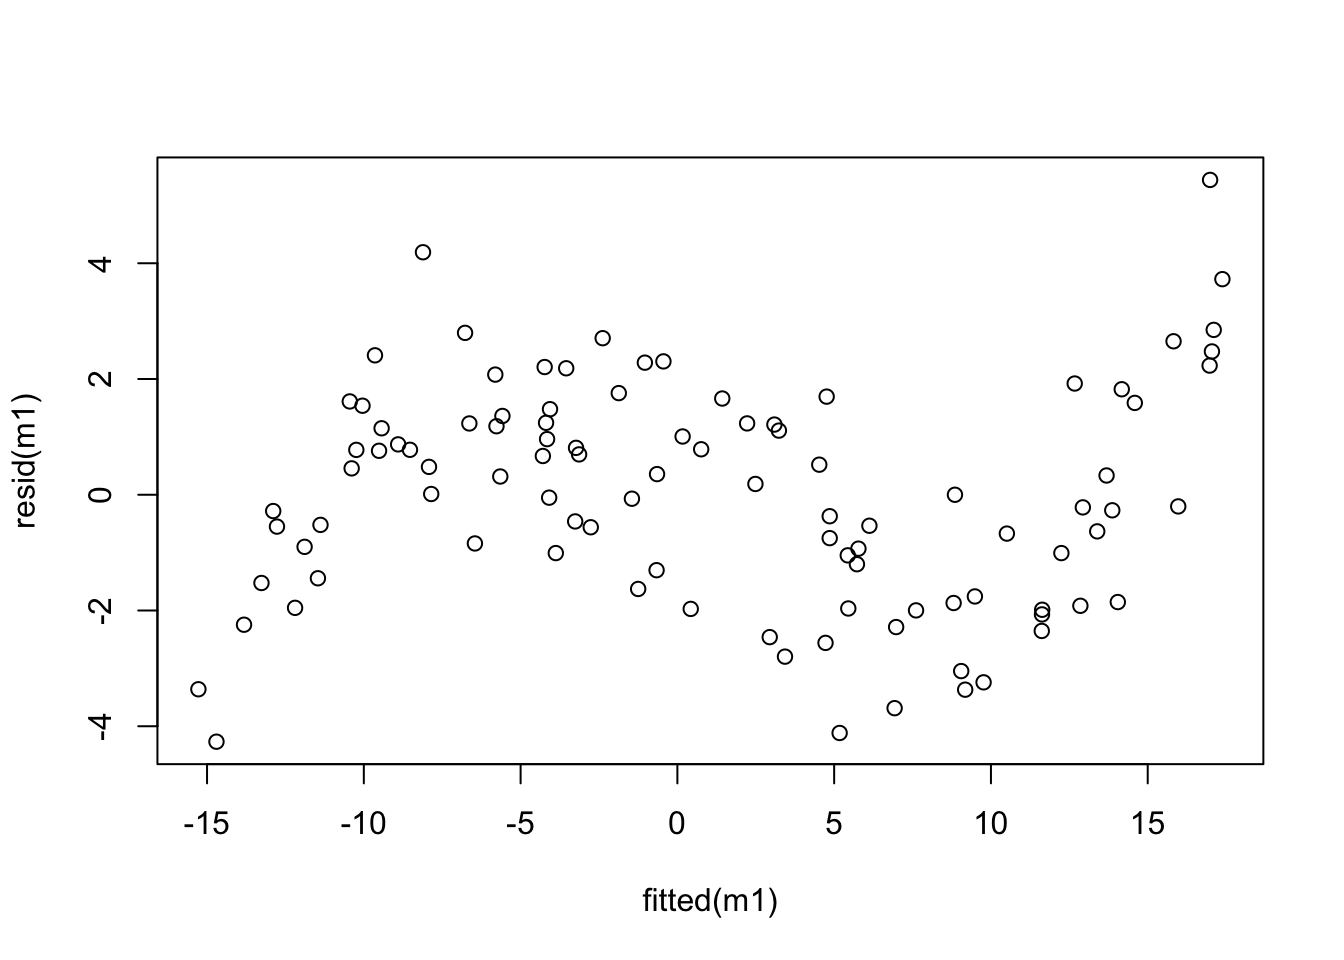
\includegraphics{MATH3714_files/figure-latex/P02Q08-1.pdf}

\begin{Shaded}
\begin{Highlighting}[]
\NormalTok{m2 }\OtherTok{\textless{}{-}} \FunctionTok{lm}\NormalTok{(y }\SpecialCharTok{\textasciitilde{}}\NormalTok{ x }\SpecialCharTok{+} \FunctionTok{I}\NormalTok{(x}\SpecialCharTok{\^{}}\DecValTok{2}\NormalTok{), }\AttributeTok{data =}\NormalTok{ d)}
\FunctionTok{plot}\NormalTok{(}\FunctionTok{fitted}\NormalTok{(m2), }\FunctionTok{resid}\NormalTok{(m2))}
\end{Highlighting}
\end{Shaded}

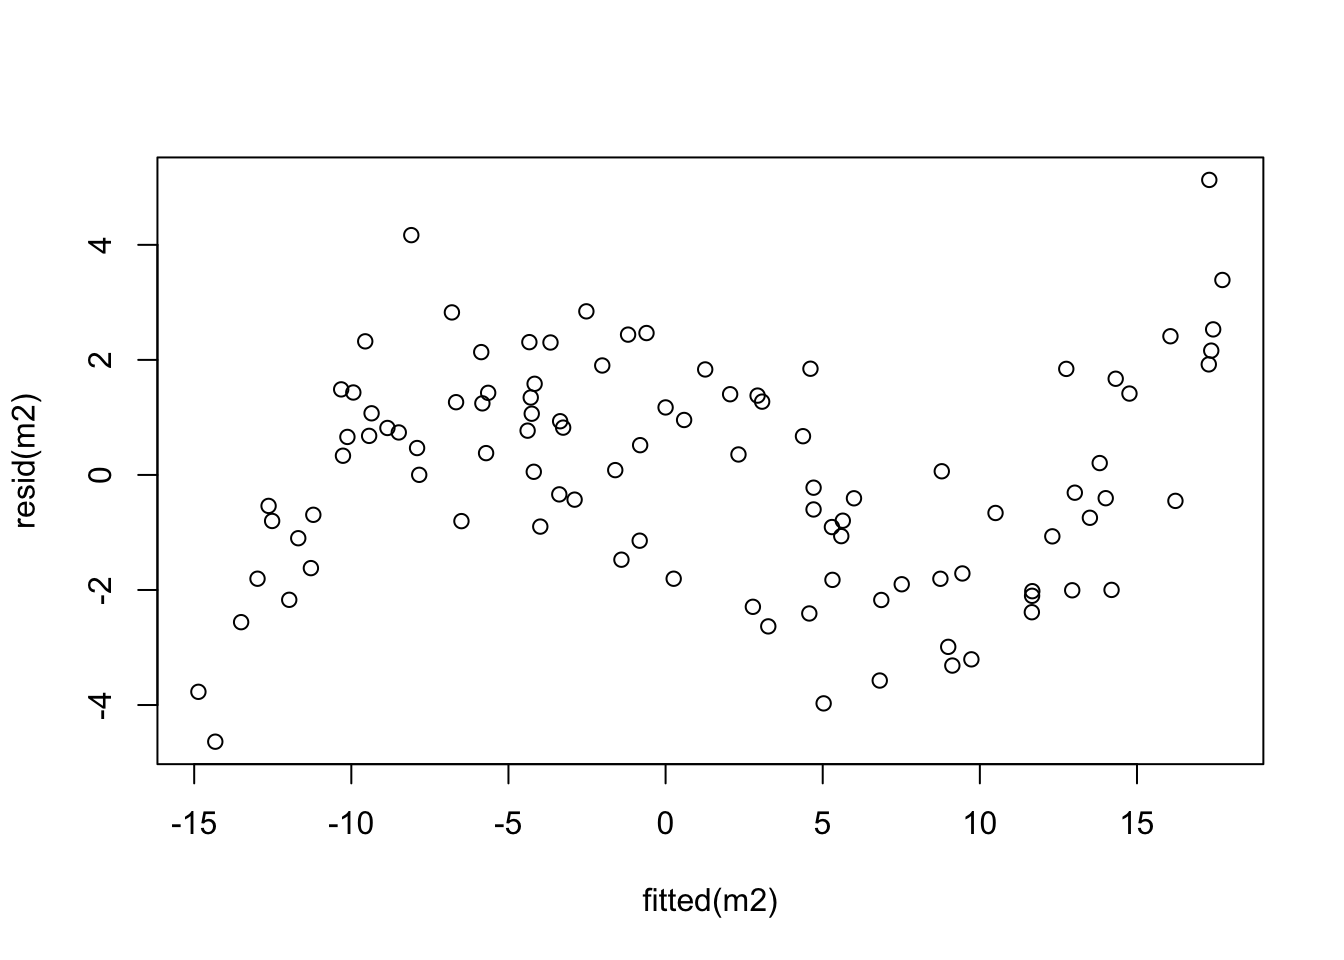
\includegraphics{MATH3714_files/figure-latex/P02Q08-2.pdf}

\begin{Shaded}
\begin{Highlighting}[]
\NormalTok{m3 }\OtherTok{\textless{}{-}} \FunctionTok{lm}\NormalTok{(y }\SpecialCharTok{\textasciitilde{}}\NormalTok{ x }\SpecialCharTok{+} \FunctionTok{I}\NormalTok{(x}\SpecialCharTok{\^{}}\DecValTok{2}\NormalTok{) }\SpecialCharTok{+} \FunctionTok{I}\NormalTok{(x}\SpecialCharTok{\^{}}\DecValTok{3}\NormalTok{), }\AttributeTok{data =}\NormalTok{ d)}
\FunctionTok{plot}\NormalTok{(}\FunctionTok{fitted}\NormalTok{(m3), }\FunctionTok{resid}\NormalTok{(m3))}
\end{Highlighting}
\end{Shaded}

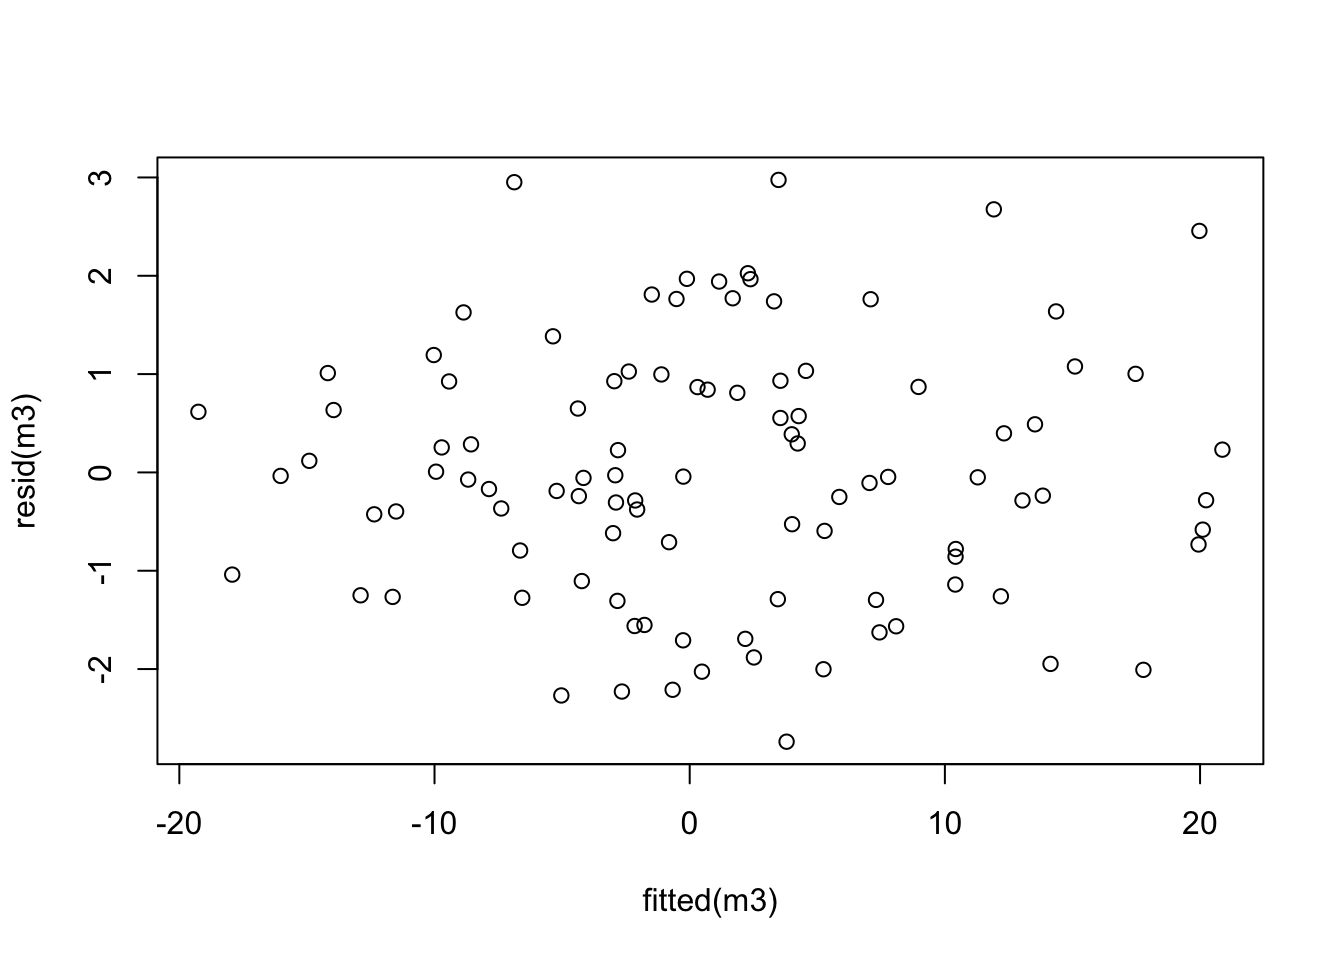
\includegraphics{MATH3714_files/figure-latex/P02Q08-3.pdf}

\end{myanswers}

\clearpage

\hypertarget{S08-diagnostics}{%
\section{Regression Diagnostics}\label{S08-diagnostics}}

The traditional principle of data analysis could be described by the following
steps

\begin{enumerate}
\def\labelenumi{\arabic{enumi}.}
\tightlist
\item
  Explore the data; identify a plausible model.
\item
  Estimate any parameters specified by the model.
\item
  Check that the model is adequate --- often by examining the discrepancy
  between the observed data and that predicted (or fitted) by the model --- if
  necessary go back a step with a refined/revised model.
\item
  See if the model can be simplified; if necessary go to step 2.
\item
  Conclude (using the results as required).
\end{enumerate}

In (multiple) regression there are many checks which can be used in step 3.
These can consider the model as a whole, or be very specific by examining each
observation, and the effect it has on the model.

\hypertarget{plots}{%
\subsection{Diagnostic Plots}\label{plots}}

The regression model is often checked by examining the residuals. Various plots
are used:

\begin{enumerate}
\def\labelenumi{\arabic{enumi}.}
\item
  A scatter plot of the response \(y\) against each of the explanatory
  variables \(x_j\) for \(j \in \{1, \ldots, p\}\).
\item
  A scatter plot of \(\hat\varepsilon\) against each of the explanatory variables
  \(x_j\) for \(j \in \{1, \ldots, p\}\). The presence of a curvilinear
  relationship (in this plot, or the ones above) suggests a higher-order term,
  perhaps a quadratic in the explanatory variable, should be added to the
  model. Or possibly a transformation.
\item
  A plot of \(\hat\varepsilon_i\) \emph{vs.} \(\hat y_i\). If the variance of the residuals
  seems to increase with \(\hat y\) then a transformation may be necessary.
\item
  A plot of \(\hat\varepsilon_i\) \emph{vs.} any explanatory variables not
  used in the model. A relationship suggests that the variable should be
  included.
\item
  A \href{https://en.wikipedia.org/wiki/Q\%E2\%80\%93Q_plot}{Q-Q plot}
  of the residuals can be used to assess whether the residuals are normally
  distributed. These plots plot quantiles of the data against quantiles
  of a normal distribution. If the residual are normally distributed,
  the points in a Q-Q plot will approximately lie on a straight line.
  (Most inference assumes that the errors are normally distributed, though
  the least squares estimate for \(\hat\beta\) itself does not.) The R
  command to produce Q-Q plots for the normal distribution is \texttt{qqnorm()}.
\item
  Data are often collected in time order. Even if time is not an explanatory
  variable, a plot of \(y\) \emph{vs.} time can be of interest. It can reveal
  serial correlation in the data. Similarly, plotting the residuals \emph{vs.}
  time.
\item
  A plot of \(x_j\) \emph{vs.} \(x_k\) for \(j\neq k\) can also be useful.
  If two or more regressors are highly correlated, we say that
  multicollinearity is present. When this occurs the least squares estimate
  \(\hat\beta\) becomes numerically unstable.
\end{enumerate}

\begin{example}
\protect\hypertarget{exm:stackloss-plot}{}\label{exm:stackloss-plot}An example for the first type of diagnostic plot would be to
plot \texttt{stack.loss} against \texttt{Water.Temp} for the \texttt{stackloss} dataset:

\begin{Shaded}
\begin{Highlighting}[]
\FunctionTok{plot}\NormalTok{(stackloss}\SpecialCharTok{$}\NormalTok{Water.Temp, stackloss}\SpecialCharTok{$}\NormalTok{stack.loss,}
     \AttributeTok{xlab =} \StringTok{"water temperature"}\NormalTok{, }\AttributeTok{ylab =} \StringTok{"Stack loss"}\NormalTok{)}
\end{Highlighting}
\end{Shaded}

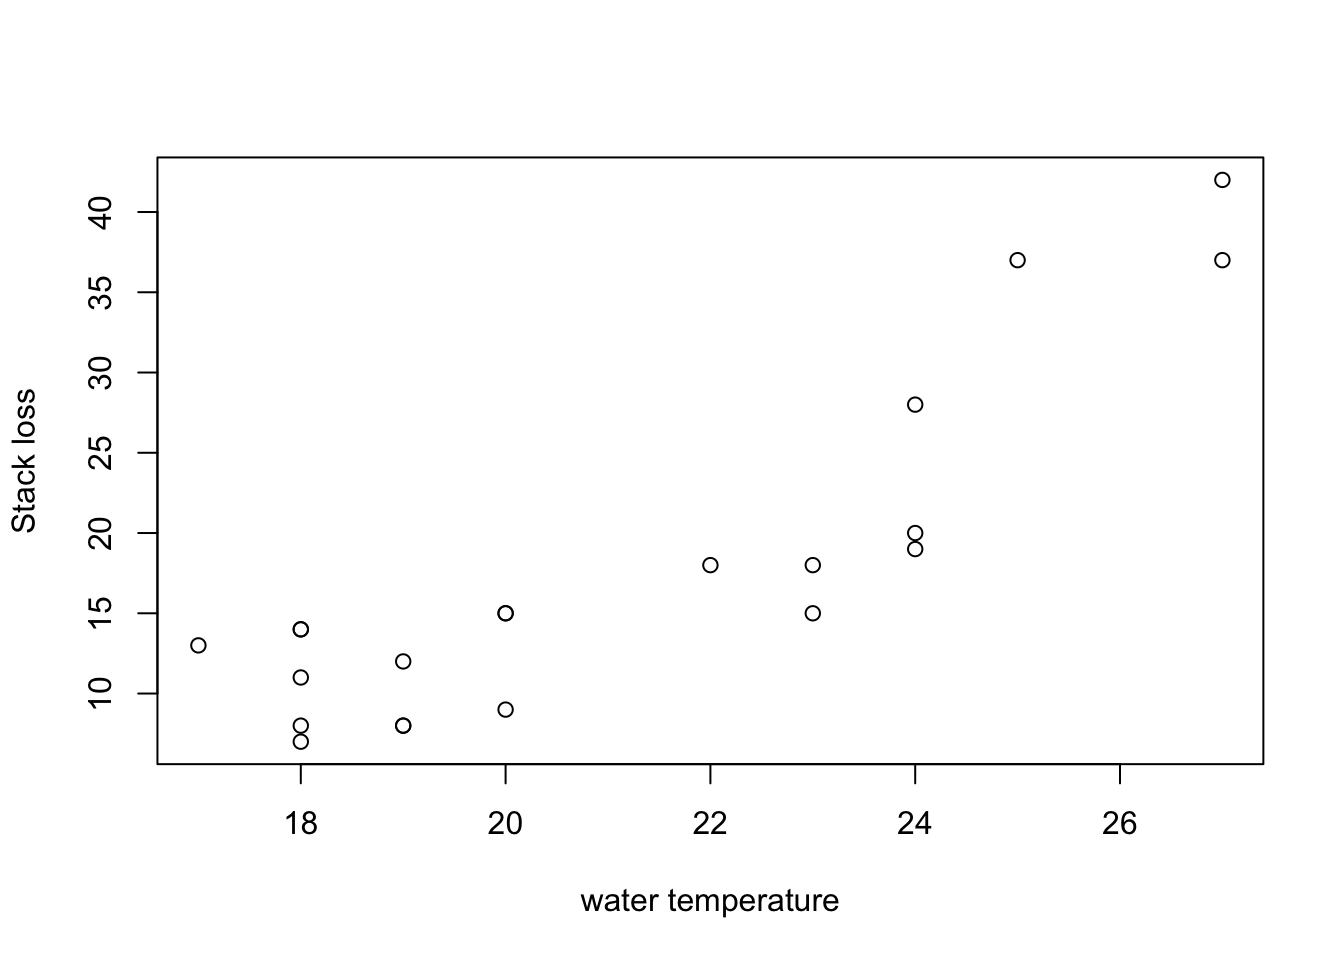
\includegraphics{MATH3714_files/figure-latex/stackloss-plot-1.pdf}

Clearly the stack loss increases with water temperature, but the
relationship may not be linear. It may make sense to include
the square of the water temperature as an additional input variable
in the model.
\end{example}

\hypertarget{R-squared}{%
\subsection{The Coefficient of Multiple Determination}\label{R-squared}}

In equation~\eqref{eq:eps-y-orth} we have seen that
\begin{equation*}
  \|y\|^2
  = \|\hat y\|^2 + \|\hat\varepsilon\|^2.
\end{equation*}
The following lemma shows that a similar relation also holds after the sample
means are subtracted.

\begin{lemma}
\protect\hypertarget{lem:explained-variance}{}\label{lem:explained-variance}Assume that the fitted model includes an intercept. Then we have
\begin{align*}
  \sum_{i=1}^n (y_i - \overline{y})^2
  &= \sum_{i=1}^n (\hat y_i - \overline{y})^2
    + \sum_{i=1}^n \hat \varepsilon_i^2 \\
  &= \sum_{i=1}^n \bigl( \hat y_i - \overline{\hat y} \bigr)^2
    + \sum_{i=1}^n \bigl( \hat \varepsilon_i - \overline{\hat\varepsilon} \bigr)^2,
\end{align*}
where \(\overline{y}\), \(\overline{\hat y}\) and \(\overline{\hat\varepsilon}\)
are the sample means of the three vectors \(y\), \(\hat y\) and~\(\hat\varepsilon\).
\end{lemma}

\begin{proof}
Define \(\mathbf{1} = (1, \ldots, 1) \in \mathbb{R}^p\). From exercise~2 on
problem sheet 1 we know that \(H\mathbf{1} = \mathbf{1}\) and since \(H\)
is symmetric we also have \(\mathbf{1}^\top H = \mathbf{1}^\top\).
This gives
\begin{equation}
  \mathbf{1}^\top (I - H)
  = \mathbf{1}^\top - \mathbf{1}^\top H
  = \mathbf{1}^\top - \mathbf{1}^\top
  = 0.  \label{eq:I-H-left}
\end{equation}

As we have already seen previously, we have
\begin{align*}
  \hat y^\top \hat\varepsilon
  &= (H y)^\top (I - H) y \\
  &= y^\top H (I - H) y \\
  &= 0
\end{align*}
and using equation~\eqref{eq:I-H-left} we also get
\begin{equation}
  \mathbf{1}^\top \hat\varepsilon
  = \mathbf{1}^\top (I - H) y
  = 0.
\end{equation}
Thus, \((\hat y - \overline{y} \mathbf{1})^\top \hat\varepsilon= 0\) and using
Pythagoras' theorem as in the section about \protect\hyperlink{hat-matrix}{Properties of the Hat Matrix}, we
find
\begin{align*}
  \| y - \overline{y} \mathbf{1} \|^2
  &= \| y - \hat y + \hat y - \overline{y} \mathbf{1} \|^2 \\
  &= \| \hat \varepsilon+ \hat y - \overline{y} \mathbf{1} \|^2 \\
  &= \| \hat \varepsilon\|^2 + \| \hat y - \overline{y} \mathbf{1} \|^2.
\end{align*}
This proves the first equality.

Using equation~\eqref{eq:I-H-left} again, we find
\begin{equation*}
  \sum_{i=1}^n \hat\varepsilon_i
  = \mathbf{1}^\top \hat\varepsilon
  = \mathbf{1}^\top (y - \hat y)
  = \mathbf{1}^\top (I - H) y
  = 0
\end{equation*}
and thus \(\overline{\hat\varepsilon} = 0\).
Since \(y = \hat y + (y - \hat y) = \hat y + \hat\varepsilon\) we also have
\begin{equation*}
  \overline{y}
  = \overline{\hat y} + \overline{\hat\varepsilon}
  = \overline{\hat y}.
\end{equation*}
This completes the proof.
\end{proof}

We can express the terms in the statement of lemma~\ref{lem:explained-variance}
as sample variances. For example, we write
\begin{equation*}
  \mathrm{s}_y^2
  = \frac{1}{n-1} \sum_{i=1}^n (y_i - \bar y)^2
\end{equation*}
for the sample variance of~\(y\). Using this notation, the statement of
the lemma can be written as
\begin{equation*}
  \mathrm{s}_y^2
  = \mathrm{s}_{\hat y}^2 + \mathrm{s}_{\hat\varepsilon}^2.
\end{equation*}
Different from equation~\eqref{eq:eps-y-orth}, the current relation is
only true for models which include an intercept.

Some authors define

\begin{itemize}
\tightlist
\item
  \(\mathrm{SS}_\mathrm{tot} = \sum_{i=1}^n (y_i - \bar y)^2\)
  (where ``tot'' stands for ``total'')
\item
  \(\mathrm{SS}_\mathrm{reg} = \sum_{i=1}^n (\hat y_i - \overline{\hat y})^2\)
  (where ``reg'' stands for ``regression'')
\item
  \(\mathrm{SS}_\mathrm{res} = \sum_{i=1}^n (y_i-\hat y_i)^2\)
  (where ``res'' stands for ``residual'')
\end{itemize}

Using this notation, the statement of lemma~\ref{lem:explained-variance}
becomes
\begin{equation*}
  \mathrm{SS}_\mathrm{tot}
  = \mathrm{SS}_\mathrm{reg} + \mathrm{SS}_\mathrm{res}.
\end{equation*}

\begin{definition}
\protect\hypertarget{def:R-squared}{}\label{def:R-squared}The \textbf{coefficient of multiple determination} is defined to be
\begin{equation*}
  R^2
  := 1 - \frac{\mathrm{s}_{\hat\varepsilon}^2}{\mathrm{s}_y^2}
  = 1 - \frac{\sum_{i=1}^n \hat\varepsilon_i^2}{\sum_{i=1}^n (y_i - \bar y)^2}.
\end{equation*}
\end{definition}

Using the result of lemma~\ref{lem:explained-variance}, for models which
include an intercept we can also
express \(R^2\) as
\begin{equation*}
  R^2
  = \mathrm{s}_{\hat y}^2 / \mathrm{s}_y^2.
\end{equation*}
Since both numerator and denominator are positive, if is clear the \(R^2 \geq 0\). Similarly, from the definition it is clear that \(R^2 \leq 1\), so that we
always have \(R^2 \in [0, 1]\). A large value of \(R^2\) indicates that
the residuals are small, compared to the sample variance of the \(y_i\)
and thus often indicates good model fit.

\begin{example}

We can easily compute the \(R^2\) value for the \texttt{stackloss} dataset
manually:

\begin{Shaded}
\begin{Highlighting}[]
\NormalTok{m }\OtherTok{\textless{}{-}} \FunctionTok{lm}\NormalTok{(stack.loss }\SpecialCharTok{\textasciitilde{}}\NormalTok{ ., }\AttributeTok{data =}\NormalTok{ stackloss)}
\NormalTok{R.squared }\OtherTok{\textless{}{-}} \DecValTok{1} \SpecialCharTok{{-}} \FunctionTok{var}\NormalTok{(}\FunctionTok{resid}\NormalTok{(m)) }\SpecialCharTok{/} \FunctionTok{var}\NormalTok{(stackloss}\SpecialCharTok{$}\NormalTok{stack.loss)}
\NormalTok{R.squared}
\end{Highlighting}
\end{Shaded}

\begin{Shaded}
\begin{Highlighting}[]
\NormalTok{\# [1] 0.9135769}
\end{Highlighting}
\end{Shaded}

We can also find this value near the bottom of the output of
\texttt{summary(m)}, listed as \texttt{Multiple\ R-squared}:

\begin{Shaded}
\begin{Highlighting}[]
\FunctionTok{summary}\NormalTok{(m)}
\end{Highlighting}
\end{Shaded}

\begin{Shaded}
\begin{Highlighting}[]
\NormalTok{\# }
\NormalTok{\# Call:}
\NormalTok{\# lm(formula = stack.loss \textasciitilde{} ., data = stackloss)}
\NormalTok{\# }
\NormalTok{\# Residuals:}
\NormalTok{\#     Min      1Q  Median      3Q     Max }
\NormalTok{\# {-}7.2377 {-}1.7117 {-}0.4551  2.3614  5.6978 }
\NormalTok{\# }
\NormalTok{\# Coefficients:}
\NormalTok{\#             Estimate Std. Error t value Pr(\textgreater{}|t|)    }
\NormalTok{\# (Intercept) {-}39.9197    11.8960  {-}3.356  0.00375 ** }
\NormalTok{\# Air.Flow      0.7156     0.1349   5.307  5.8e{-}05 ***}
\NormalTok{\# Water.Temp    1.2953     0.3680   3.520  0.00263 ** }
\NormalTok{\# Acid.Conc.   {-}0.1521     0.1563  {-}0.973  0.34405    }
\NormalTok{\# {-}{-}{-}}
\NormalTok{\# Signif. codes:  0 \textquotesingle{}***\textquotesingle{} 0.001 \textquotesingle{}**\textquotesingle{} 0.01 \textquotesingle{}*\textquotesingle{} 0.05 \textquotesingle{}.\textquotesingle{} 0.1 \textquotesingle{} \textquotesingle{} 1}
\NormalTok{\# }
\NormalTok{\# Residual standard error: 3.243 on 17 degrees of freedom}
\NormalTok{\# Multiple R{-}squared:  0.9136,  Adjusted R{-}squared:  0.8983 }
\NormalTok{\# F{-}statistic:  59.9 on 3 and 17 DF,  p{-}value: 3.016e{-}09}
\end{Highlighting}
\end{Shaded}

\end{example}

One problem with the \(R^2\) value is, that it always increases when another
input variable is added to the model. Thus, the \(R^2\) value cannot be used
to compare model fit for models with different numbers of variables. An
attempt to compensate for this effect is the adjusted \(R^2\) value:

\begin{definition}
\protect\hypertarget{def:adjusted-R-squared}{}\label{def:adjusted-R-squared}The \textbf{adjusted \(R^2\) value} is given by
\begin{equation*}
  R^2_\mathrm{adj}
  := 1 - \frac{\frac{1}{n-p-1}\mathrm{s}_{\hat\varepsilon}^2}{\frac{1}{n-1}\mathrm{s}_y^2}
  = 1 - \frac{n-1}{n-p-1}(1 - R^2).
\end{equation*}
\end{definition}

The value \(R^2_\mathrm{adj}\) is always smaller than the \(R^2\) value, and
\(R^2_\mathrm{adj}\) can be (slightly) negative.

\begin{example}
The adjusted \(R^2\) value for the stackloss dataset
can be found as follows:

\begin{Shaded}
\begin{Highlighting}[]
\NormalTok{n }\OtherTok{\textless{}{-}} \FunctionTok{nrow}\NormalTok{(stackloss)}
\NormalTok{p }\OtherTok{\textless{}{-}} \FunctionTok{ncol}\NormalTok{(stackloss) }\SpecialCharTok{{-}} \DecValTok{1}
\NormalTok{R.squared.adj }\OtherTok{\textless{}{-}} \DecValTok{1} \SpecialCharTok{{-}}\NormalTok{ (n }\SpecialCharTok{{-}} \DecValTok{1}\NormalTok{) }\SpecialCharTok{/}\NormalTok{ (n }\SpecialCharTok{{-}}\NormalTok{ p }\SpecialCharTok{{-}} \DecValTok{1}\NormalTok{) }\SpecialCharTok{*}\NormalTok{ (}\DecValTok{1} \SpecialCharTok{{-}}\NormalTok{ R.squared)}
\NormalTok{R.squared.adj}
\end{Highlighting}
\end{Shaded}

\begin{Shaded}
\begin{Highlighting}[]
\NormalTok{\# [1] 0.8983258}
\end{Highlighting}
\end{Shaded}

We can also find this value near the bottom of the output of
\texttt{summary(m)}, listed as \texttt{Adjusted\ R-squared}.
\end{example}

\begin{example}
As suggested in example~\ref{exm:stackloss-plot}, we may want to
include a new quadratic term in the stackloss dataset:

\begin{Shaded}
\begin{Highlighting}[]
\NormalTok{m2 }\OtherTok{\textless{}{-}} \FunctionTok{lm}\NormalTok{(stack.loss }\SpecialCharTok{\textasciitilde{}}\NormalTok{ . }\SpecialCharTok{+} \FunctionTok{I}\NormalTok{(Water.Temp}\SpecialCharTok{\^{}}\DecValTok{2}\NormalTok{), }\AttributeTok{data =}\NormalTok{ stackloss)}
\FunctionTok{summary}\NormalTok{(m2)}
\end{Highlighting}
\end{Shaded}

\begin{Shaded}
\begin{Highlighting}[]
\NormalTok{\# }
\NormalTok{\# Call:}
\NormalTok{\# lm(formula = stack.loss \textasciitilde{} . + I(Water.Temp\^{}2), data = stackloss)}
\NormalTok{\# }
\NormalTok{\# Residuals:}
\NormalTok{\#     Min      1Q  Median      3Q     Max }
\NormalTok{\# {-}4.1217 {-}1.5205 {-}0.3091  0.9753  6.0554 }
\NormalTok{\# }
\NormalTok{\# Coefficients:}
\NormalTok{\#                 Estimate Std. Error t value Pr(\textgreater{}|t|)   }
\NormalTok{\# (Intercept)     57.73727   46.08487   1.253  0.22826   }
\NormalTok{\# Air.Flow         0.53683    0.14708   3.650  0.00216 **}
\NormalTok{\# Water.Temp      {-}7.62030    4.10441  {-}1.857  0.08188 . }
\NormalTok{\# Acid.Conc.      {-}0.09697    0.14371  {-}0.675  0.50946   }
\NormalTok{\# I(Water.Temp\^{}2)  0.21224    0.09738   2.179  0.04459 * }
\NormalTok{\# {-}{-}{-}}
\NormalTok{\# Signif. codes:  0 \textquotesingle{}***\textquotesingle{} 0.001 \textquotesingle{}**\textquotesingle{} 0.01 \textquotesingle{}*\textquotesingle{} 0.05 \textquotesingle{}.\textquotesingle{} 0.1 \textquotesingle{} \textquotesingle{} 1}
\NormalTok{\# }
\NormalTok{\# Residual standard error: 2.936 on 16 degrees of freedom}
\NormalTok{\# Multiple R{-}squared:  0.9334,  Adjusted R{-}squared:  0.9167 }
\NormalTok{\# F{-}statistic: 56.02 on 4 and 16 DF,  p{-}value: 3.293e{-}09}
\end{Highlighting}
\end{Shaded}

As expected, the \(R^2\) value has increased here (from 0.9136 to 0.9334).
Since the adjusted \(R^2\) value has also increased (from 0.8983 to 0.9167),
the extended model may be better than the original model.
\end{example}

\clearpage

\hypertarget{S09-influence}{%
\section{The Influence of Observations}\label{S09-influence}}

In this section we consider the influence which individual samples have on
the estimate. Samples with a large influence may be outliers, and are
worth checking for validity.

\hypertarget{deleting-observations}{%
\subsection{Deleting Observations}\label{deleting-observations}}

The most direct way to check for the influence of an observation
is to compute the parameter estimate \(\hat\beta\) both with and without
the observation in question, and to see how much the two results differ.

\begin{definition}
For \(I \subset \{1, \ldots, n\}\) we write~\(\hat\beta^{(I)}\) for the estimate
where all observations \(i\in I\) have been removed. As a shorthand we write
\(\hat\beta^{(i)}\) instead of \(\hat\beta^{(\{i\})}\) for the case where only
a single observation has been removed.
\end{definition}

This approach is very different from what we used in the
section about \protect\hyperlink{S06-simultaneous}{Estimating Coefficients Simultaneously}. There, we selected a
subset of regression coefficients, corresponding to columns in the design
matrix~\(X\), whereas here we are considering a subset of the observations,
corresponding to rows of~\(X\).

Using the formula for the least squares estimate, we know that
\begin{equation}
  \hat\beta^{(I)}
  = (X_{(I)}^\top X_{(I)})^{-1} X_{(I)}^\top y,  \label{eq:hat-beta-I1}
\end{equation}
where now \(X_{(I)}\) is \(X\) with all rows \(i\in I\) removed. (We write the
``\((I)\)'' as a subscript, to make space for the transpose sign.) Our first aim
is to find an explicit formula for the difference between \(\hat\beta\) and
\(\hat\beta^{(I)}\).

We have
\begin{align*}
  (X_{(I)}^\top y)_k
  &= \sum_{j \notin I} X_{jk} y_j \\
  &= \sum_{j=1}^n X_{jk} y_j - \sum_{j\in I} X_{jk} y_j
\end{align*}
for all \(k \in \{0, \ldots, p\}\), and thus
\begin{equation}
  X_{(I)}^\top y
  = X^\top y - X_I^\top y_I,  \label{eq:X-I-top-y}
\end{equation}
where \(X_I\) stands for the matrix which only contains the rows \(i\in I\) of~the
matrix \(X\), and \(y_I = (y_i)_{i\in I}\). Before we substitute this result into
equation~\eqref{eq:hat-beta-I1}, we first consider how we can write the the
inverse \((X_{(I)}^\top X_{(I)})^{-1}\) in terms of \((X^\top X)^{-1}\).

\begin{lemma}
\protect\hypertarget{lem:low-rank-inverse}{}\label{lem:low-rank-inverse}Let \(A \in \mathbb{R}^{(p+1)\times (p+1)}\) and let \(U, V \in \mathbb{R}^{m \times (p+1)}\).
Then
\begin{equation*}
  (A - U^\top V)^{-1}
  = A^{-1} + A^{-1} U^\top (I - V A^{-1} U^\top)^{-1} V A^{-1}.
\end{equation*}
\end{lemma}

\begin{proof}
This statement is proved by multiplying the equation with \(A - U^\top V\).
Expanding all brackets and using the relation \(A A^{-1} = I\), we find
\begin{equation*}
  \bigl( A - U^\top V \bigr)
    \bigl( A^{-1} + A^{-1} U^\top (I - V A^{-1} U^\top)^{-1} V A^{-1} \bigr)
  = \cdots
  = I.
\end{equation*}
This shows that we have indeed found the inverse of~\(A - U^\top V\).
\end{proof}

Using this result, we can now derive a formula for the change in \(\hat\beta\)
when some observations are omitted.

\begin{lemma}
\protect\hypertarget{lem:hat-beta-I}{}\label{lem:hat-beta-I}We have
\begin{equation*}
  \hat\beta^{(I)} - \hat\beta
  = - (X^\top X)^{-1} X_I^\top (I - H_{II})^{-1} \hat\varepsilon_I,
\end{equation*}
where \(H_{II} := X_I (X^\top X)^{-1} X_I^\top = (h_{ij})_{i,j\in I}\) is the
matrix which contains the elements of the hat matrix~\(H\) where both row and
column are in \(I\), and \(\hat\varepsilon_I = (\hat\varepsilon_i)_{i\in I} = (y_i - \hat y_i)_{i\in I}\) is the vector of residuals at the omitted samples.
\end{lemma}

The vector \(\hat\varepsilon_I\) consists of a subset of the original
residuals, computed using the original \(\hat y\) and \(\hat\beta\). It does not
refer to the modified estimate \(\hat\beta^{(I)}\) which was computing with some
observations omitted. Similarly, \(H_{II}\) is a submatrix of the original
hat matrix.

\begin{proof}
Similar to \eqref{eq:X-I-top-y}, we
\begin{equation*}
  (X_{(I)}^\top X_{(I)})_{ik}
  = \sum_{j\notin I} X_{ji} X_{jk}
  = \sum_{j=1}^n X_{ji} X_{jk} - \sum_{j\in I} X_{ji} X_{jk}
\end{equation*}
and thus
\begin{equation*}
  X_{(I)}^\top X_{(I)}
  = X^\top X - X_I^\top X_I.
\end{equation*}
Now we can use the lemma with \(U = V = X_I\) to get
\begin{align*}
  (X_{(I)}^\top X_{(I)})^{-1}
  &= (X^\top X)^{-1} + (X^\top X)^{-1} X_I^\top (I - X_I (X^\top X)^{-1} X_I^\top)^{-1} X_I (X^\top X)^{-1} \\
  &= (X^\top X)^{-1} + (X^\top X)^{-1} X_I^\top (I - H_{II})^{-1} X_I (X^\top X)^{-1}.
\end{align*}

Using equations \eqref{eq:hat-beta-I1} and~\eqref{eq:X-I-top-y} and
lemma~\ref{lem:low-rank-inverse} we get
\begin{align*}
  \hat\beta^{(I)}
  &= (X_{(I)}^\top X_{(I)})^{-1} X_{(I)}^\top y \\
  &= (X_{(I)}^\top X_{(I)})^{-1} (X^\top y - X_I^\top y_I) \\
  &= \Bigl( (X^\top X)^{-1} + (X^\top X)^{-1} X_I^\top (I - H_{II})^{-1} X_I (X^\top X)^{-1} \Bigr) (X^\top y - X_I^\top y_I) \\
  &= (X^\top X)^{-1} X^\top y \\
    &\hskip1cm + (X^\top X)^{-1} X_I^\top (I - H_{II})^{-1} X_I \hat\beta \\
    &\hskip1cm - (X^\top X)^{-1} X_I^\top y_I \\
    &\hskip1cm - (X^\top X)^{-1} X_I^\top (I - H_{II})^{-1} X_I (X^\top X)^{-1} X_I^\top y_I \\
  &= \hat\beta
               + (X^\top X)^{-1} X_I^\top (I - H_{II})^{-1} X_I \hat\beta \\
    &\hskip1cm - (X^\top X)^{-1} X_I^\top (I - H_{II})^{-1} (I - H_{II}) y_I \\
    &\hskip1cm - (X^\top X)^{-1} X_I^\top (I - H_{II})^{-1} H_{II} y_I \\
  &= \hat\beta
               + (X^\top X)^{-1} X_I^\top (I - H_{II})^{-1} X_I \hat\beta \\
    &\hskip1cm - (X^\top X)^{-1} X_I^\top (I - H_{II})^{-1} y_I \\
  &= \hat\beta - (X^\top X)^{-1} X_I^\top (I - H_{II})^{-1} \bigl( y_I -  X_I \hat\beta \bigr) \\
  &= \hat\beta - (X^\top X)^{-1} X_I^\top (I - H_{II})^{-1} \hat\varepsilon_I.
\end{align*}
This completes the proof.
\end{proof}

We can also find the change in estimated error variance, when samples
are omitted from the estimate. The estimated variance in the modified model
is
\begin{align*}
  \hat\sigma_{(I)}^2
  &:= \frac{1}{n-m-p-1} \sum_{i\notin I} \Bigl( y_i - (X\hat\beta^{(I)})_i \Bigr)^2 \\
  &= \frac{1}{n-m-p-1} \Bigl\| y_{(I)} - X_{(I)} \hat\beta^{(I)} \Bigr\|^2
\end{align*}
where \(m = |I|\) so that \(n-m\) is the number of observations used
in the estimate. We want to compare this quantity to the original estimate
\begin{align*}
  \hat\sigma^2
  &= \frac{1}{n-p-1} \sum_{i=1}^n \Bigl( y_i - (X\hat\beta)_i \Bigr)^2 \\
  &= \frac{1}{n-p-1} \Bigl\| y - X \hat\beta \Bigr\|^2.
\end{align*}
Here we used again the Euclidean norm as a shorthand for the sum of squares
used in these estimates. The following lemma shows how the residual sum
of squares decreases when the observations \(I\) are omitted from the
estimate.

\begin{lemma}
\protect\hypertarget{lem:sigma-I}{}\label{lem:sigma-I}We have
\begin{equation*}
  \| y_{(I)} - X_{(I)} \hat\beta^{(I)} \|^2 - \| y - \hat y \|^2
  = - \hat\varepsilon_I^\top (I - H_{II})^{-1} \hat\varepsilon_I.
\end{equation*}
\end{lemma}

The proof of this lemma is similar to the proof of lemma~\ref{lem:hat-beta-I},
but we omit the tedious calculations here.

\begin{example}
To illustrate the results of this subsection, we give a numerical example.
In the example we consider the \texttt{stackloss} dataset, and study what happens
when the first two observations are omitted:

\begin{Shaded}
\begin{Highlighting}[]
\NormalTok{m1 }\OtherTok{\textless{}{-}} \FunctionTok{lm}\NormalTok{(stack.loss }\SpecialCharTok{\textasciitilde{}}\NormalTok{ ., }\AttributeTok{data =}\NormalTok{ stackloss)}
\NormalTok{m2 }\OtherTok{\textless{}{-}} \FunctionTok{lm}\NormalTok{(stack.loss }\SpecialCharTok{\textasciitilde{}}\NormalTok{ ., }\AttributeTok{data =}\NormalTok{ stackloss[}\SpecialCharTok{{-}}\FunctionTok{c}\NormalTok{(}\DecValTok{1}\NormalTok{,}\DecValTok{2}\NormalTok{),])}
\FunctionTok{coef}\NormalTok{(m2) }\SpecialCharTok{{-}} \FunctionTok{coef}\NormalTok{(m1)}
\end{Highlighting}
\end{Shaded}

\begin{Shaded}
\begin{Highlighting}[]
\NormalTok{\# (Intercept)    Air.Flow  Water.Temp  Acid.Conc. }
\NormalTok{\#  0.86331016 {-}0.03780761 {-}0.02706305  0.02124533}
\end{Highlighting}
\end{Shaded}

Using the result of lemma~\ref{lem:hat-beta-I}, we can get the difference
between the two estimates without using the model \texttt{m2}:

\begin{Shaded}
\begin{Highlighting}[]
\NormalTok{X }\OtherTok{\textless{}{-}} \FunctionTok{model.matrix}\NormalTok{(m1)}
\NormalTok{H }\OtherTok{\textless{}{-}}\NormalTok{ X }\SpecialCharTok{\%*\%} \FunctionTok{solve}\NormalTok{(}\FunctionTok{t}\NormalTok{(X) }\SpecialCharTok{\%*\%}\NormalTok{ X, }\FunctionTok{t}\NormalTok{(X))}
\NormalTok{XI }\OtherTok{\textless{}{-}}\NormalTok{ X[}\DecValTok{1}\SpecialCharTok{:}\DecValTok{2}\NormalTok{,]}
\NormalTok{hII }\OtherTok{\textless{}{-}}\NormalTok{ H[}\DecValTok{1}\SpecialCharTok{:}\DecValTok{2}\NormalTok{, }\DecValTok{1}\SpecialCharTok{:}\DecValTok{2}\NormalTok{]}
\NormalTok{hat.epsI }\OtherTok{\textless{}{-}} \FunctionTok{resid}\NormalTok{(m1)[}\DecValTok{1}\SpecialCharTok{:}\DecValTok{2}\NormalTok{]}

\SpecialCharTok{{-}}\FunctionTok{as.vector}\NormalTok{(}\FunctionTok{solve}\NormalTok{(}\FunctionTok{t}\NormalTok{(X) }\SpecialCharTok{\%*\%}\NormalTok{ X) }\SpecialCharTok{\%*\%} \FunctionTok{t}\NormalTok{(XI) }\SpecialCharTok{\%*\%} \FunctionTok{solve}\NormalTok{(}\FunctionTok{diag}\NormalTok{(}\DecValTok{2}\NormalTok{) }\SpecialCharTok{{-}}\NormalTok{ hII, hat.epsI))}
\end{Highlighting}
\end{Shaded}

\begin{Shaded}
\begin{Highlighting}[]
\NormalTok{\# [1]  0.86331016 {-}0.03780761 {-}0.02706305  0.02124533}
\end{Highlighting}
\end{Shaded}

This is the same result as we obtained above. (I used \texttt{as.vector()} to
convert the result from a \(4\times 1\) matrix into a vector.)

Similarly, we can compare the residual sum of squares:
A direct comparison gives

\begin{Shaded}
\begin{Highlighting}[]
\FunctionTok{sum}\NormalTok{(}\FunctionTok{resid}\NormalTok{(m2)}\SpecialCharTok{\^{}}\DecValTok{2}\NormalTok{) }\SpecialCharTok{{-}} \FunctionTok{sum}\NormalTok{(}\FunctionTok{resid}\NormalTok{(m1)}\SpecialCharTok{\^{}}\DecValTok{2}\NormalTok{)}
\end{Highlighting}
\end{Shaded}

\begin{Shaded}
\begin{Highlighting}[]
\NormalTok{\# [1] {-}15.41758}
\end{Highlighting}
\end{Shaded}

Using the result of lemma~\ref{lem:sigma-I}, we get the same result
without requiring \texttt{m2}:

\begin{Shaded}
\begin{Highlighting}[]
\SpecialCharTok{{-}}\FunctionTok{t}\NormalTok{(hat.epsI) }\SpecialCharTok{\%*\%} \FunctionTok{solve}\NormalTok{(}\FunctionTok{diag}\NormalTok{(}\DecValTok{2}\NormalTok{) }\SpecialCharTok{{-}}\NormalTok{ hII, hat.epsI)}
\end{Highlighting}
\end{Shaded}

\begin{Shaded}
\begin{Highlighting}[]
\NormalTok{\#           [,1]}
\NormalTok{\# [1,] {-}15.41758}
\end{Highlighting}
\end{Shaded}

Again, the results using both methods agree.
\end{example}

In the special case of \(m = 1\), where \(I = \{i\}\) for some
\(i \in \{1, \ldots, n\}\), our results simplify to
\begin{equation}
  \hat\beta^{(i)} - \hat\beta
    = - (X^\top X)^{-1} x_i \frac{\hat\varepsilon_i}{1 - h_{ii}} \label{eq:dbeta-i}
\end{equation}
and
\begin{equation*}
  \| y_{(i)} - x_i^\top \hat\beta^{(i)} \|^2 - \| y - \hat y \|^2
    = - \frac{\hat\varepsilon_i^2}{1 - h_{ii}},
\end{equation*}
where \(x_i \in \mathbb{R}^{p+1}\) is the \(i\)th row of \(X\) as a vector,
\(\hat\varepsilon_i\) is the usual \(i\)th residual,
and \(h_{ii}\) is the \(i\)th diagonal element of the hat matrix.
Using the correct prefactors the second result gives
\begin{equation*}
  (n-p-2) \hat\sigma_{(i)}^2
    = (n-p-1)\hat\sigma^2 - \frac{\hat\varepsilon_i^2}{1 - h_{ii}}.
\end{equation*}

We can find numerical values for these quantities using
the function \texttt{influence()}:

\begin{Shaded}
\begin{Highlighting}[]
\NormalTok{x }\OtherTok{\textless{}{-}} \FunctionTok{c}\NormalTok{(}\DecValTok{1}\NormalTok{, }\DecValTok{2}\NormalTok{, }\DecValTok{3}\NormalTok{, }\DecValTok{10}\NormalTok{)}
\NormalTok{y }\OtherTok{\textless{}{-}} \FunctionTok{c}\NormalTok{(}\DecValTok{0}\NormalTok{, }\DecValTok{0}\NormalTok{, }\DecValTok{1}\NormalTok{, }\DecValTok{3}\NormalTok{)}
\NormalTok{m }\OtherTok{\textless{}{-}} \FunctionTok{lm}\NormalTok{(y }\SpecialCharTok{\textasciitilde{}}\NormalTok{ x, }\AttributeTok{data =}\NormalTok{ stackloss)}
\FunctionTok{influence}\NormalTok{(m)}
\end{Highlighting}
\end{Shaded}

\begin{Shaded}
\begin{Highlighting}[]
\NormalTok{\# $hat}
\NormalTok{\#    1    2    3    4 }
\NormalTok{\# 0.43 0.33 0.27 0.97 }
\NormalTok{\# }
\NormalTok{\# $coefficients}
\NormalTok{\#   (Intercept)            x}
\NormalTok{\# 1  0.01719298 {-}0.002105263}
\NormalTok{\# 2 {-}0.19582090  0.019104478}
\NormalTok{\# 3  0.15369863 {-}0.009315068}
\NormalTok{\# 4  0.30666667 {-}0.160000000}
\NormalTok{\# }
\NormalTok{\# $sigma}
\NormalTok{\#         1         2         3         4 }
\NormalTok{\# 0.4682929 0.2591605 0.2482818 0.4082483 }
\NormalTok{\# }
\NormalTok{\# $wt.res}
\NormalTok{\#     1     2     3     4 }
\NormalTok{\#  0.02 {-}0.32  0.34 {-}0.04}
\end{Highlighting}
\end{Shaded}

The output lists the diagonal elements \(h_{ii}\) of the hat matrix
as \texttt{\$hat}, the vectors \(\hat\beta^{(i)} - \hat\beta\) for each \(i\)
as \texttt{\$coefficients}, the standard deviations \(\hat\sigma_{(i)}\)
for each \(i\) as \texttt{\$sigma}, and the residuals \(\hat\varepsilon_i\) as~\texttt{\$wt.res}.

\hypertarget{cooks-distance}{%
\subsection{Cook's Distance}\label{cooks-distance}}

In the section about \protect\hyperlink{S06-simultaneous}{Estimating Coefficients Simultaneously} we learned
how to measure distances of estimated parameter vectors: To compare
\(K\hat\beta\) to a vector \(K\beta\) we used the norm
\begin{equation*}
  \bigl\| K\hat\beta - K\beta \bigr\|_{K(X^\top X)^{-1}K^\top}^2
  = (K\hat\beta - K\beta)^\top \bigl(K(X^\top X)^{-1}K^\top\bigr)^{-1} (K\hat\beta - K\beta).
\end{equation*}
If we consider the full parameter vector, we can use \(K = I\) to get
\begin{equation*}
  \bigl\| \hat\beta - \beta \bigr\|_{(X^\top X)^{-1}}^2
  = (\hat\beta - \beta)^\top X^\top X (\hat\beta - \beta).
\end{equation*}
From lemma~\ref{lem:F-dist} we know that
\begin{equation*}
  F = \frac{\bigl\| \hat\beta - \beta \bigr\|_{(X^\top X)^{-1}}^2}{(p+1)\hat\sigma^2}
\end{equation*}
follows an \(F_{p+1, n-p-1}\)-distribution. We can use this measure to
quantify when the difference \(\hat\beta^{(i)} - \hat\beta\) should be
considered ``large''.

\begin{definition}
\protect\hypertarget{def:Cook-D}{}\label{def:Cook-D}\textbf{Cook's distance} for observation \(i\) is defined as
\begin{equation*}
  D_i
  = \frac{(\hat\beta^{(i)} - \hat\beta)^\top X^\top X (\hat\beta^{(i)} - \hat\beta)}{(p+1)\hat\sigma^2}.
\end{equation*}
\end{definition}

We will consider observation \(i\) to be ``influential'' if \(D_i\) is large.
Since this ``lives on the scale'' of an \(F_{p+1, n-p-1}\)-distribution,
we should compare \(D_i\) to typical values of such a distribution. For
example, we could consider the median. Here is a sample of median values
for different \(n\) and~\(p\):

\begin{Shaded}
\begin{Highlighting}[]
\NormalTok{n }\OtherTok{\textless{}{-}} \FunctionTok{c}\NormalTok{(}\DecValTok{10}\NormalTok{, }\DecValTok{30}\NormalTok{, }\DecValTok{100}\NormalTok{)}
\NormalTok{p }\OtherTok{\textless{}{-}} \FunctionTok{c}\NormalTok{(}\DecValTok{1}\NormalTok{, }\DecValTok{3}\NormalTok{, }\DecValTok{5}\NormalTok{)}
\NormalTok{xx }\OtherTok{\textless{}{-}} \FunctionTok{expand.grid}\NormalTok{(}\AttributeTok{n =}\NormalTok{ n, }\AttributeTok{p =}\NormalTok{ p)}
\FunctionTok{cbind}\NormalTok{(xx, }\AttributeTok{median =} \FunctionTok{qf}\NormalTok{(}\FloatTok{0.5}\NormalTok{, xx}\SpecialCharTok{$}\NormalTok{p }\SpecialCharTok{+} \DecValTok{1}\NormalTok{, xx}\SpecialCharTok{$}\NormalTok{n }\SpecialCharTok{{-}}\NormalTok{ xx}\SpecialCharTok{$}\NormalTok{p }\SpecialCharTok{{-}} \DecValTok{1}\NormalTok{))}
\end{Highlighting}
\end{Shaded}

\begin{Shaded}
\begin{Highlighting}[]
\NormalTok{\#     n p    median}
\NormalTok{\# 1  10 1 0.7568285}
\NormalTok{\# 2  30 1 0.7105929}
\NormalTok{\# 3 100 1 0.6980730}
\NormalTok{\# 4  10 3 0.9419133}
\NormalTok{\# 5  30 3 0.8614530}
\NormalTok{\# 6 100 3 0.8451308}
\NormalTok{\# 7  10 5 1.0616689}
\NormalTok{\# 8  30 5 0.9168687}
\NormalTok{\# 9 100 5 0.8977754}
\end{Highlighting}
\end{Shaded}

In practice, some authors suggest that an observation is ``influential''
if \(D_i > 1\), instead of using an exact quantile of the \(F\)-distribution.

The following lemma provides two additional ways to compute Cook's
distance.

\begin{lemma}
\protect\hypertarget{lem:Cook-D-alt}{}\label{lem:Cook-D-alt}We have
\begin{align*}
  D_i
  &= \frac{(\hat y^{(i)} - \hat y)^\top (\hat y^{(i)} - \hat y)}{(p+1)\hat\sigma^2} \\
  &= \frac{\hat\varepsilon_i^2}{(p+1)\hat\sigma^2} \cdot \frac{h_{ii}}{(1-h_{ii})^2}.
\end{align*}
where \(\hat y^{(i)} := X \hat\beta^{(i)}\) is the fitted value which is
predicted for observation \(i\) when this observation is not used to fit the
model, \(\hat\varepsilon_i\) are the usual residuals, and \(h_{ii}\) are the
diagonal elements of the hat matrix.
\end{lemma}

\begin{proof}
We have \(\hat y^{(i)} - \hat y = X \hat\beta^{(i)} - X \hat\beta\) and thus
\begin{equation*}
  (\hat y^{(i)} - \hat y)^\top (\hat y^{(i)} - \hat y)
  = (\hat\beta^{(i)} - \hat\beta)^\top X^\top X (\hat\beta^{(i)} - \hat\beta).
\end{equation*}
This proves the first equality. From equation~\eqref{eq:dbeta-i} we know
\begin{equation*}
  \hat\beta^{(i)} - \hat\beta
    = - (X^\top X)^{-1} x_i \frac{\hat\varepsilon_i}{1 - h_{ii}}
\end{equation*}
and thus we find
\begin{align*}
  (\hat\beta^{(i)} - \hat\beta)^\top X^\top X (\hat\beta^{(i)} - \hat\beta)
  &= \frac{\hat\varepsilon_i^2}{(1 - h_{ii})^2} x_i^\top (X^\top X)^{-1} X^\top X (X^\top X)^{-1} x_i \\
  &= \frac{\hat\varepsilon_i^2}{(1 - h_{ii})^2} x_i^\top (X^\top X)^{-1} x_i \\
  &= \frac{\hat\varepsilon_i^2}{(1 - h_{ii})^2} h_{ii}
\end{align*}
and dividing by \((p+1)\hat\sigma^2\) completes the proof.
\end{proof}

\begin{example}
To illustrate how Cook's \(D\) is computed, we use a small dataset with
simulated data. We include an \(x\)-space outlier:

\begin{Shaded}
\begin{Highlighting}[]
\FunctionTok{set.seed}\NormalTok{(}\DecValTok{20211026}\NormalTok{)}
\NormalTok{x }\OtherTok{\textless{}{-}} \FunctionTok{c}\NormalTok{(}\DecValTok{5}\NormalTok{, }\FunctionTok{seq}\NormalTok{(}\DecValTok{0}\NormalTok{, }\DecValTok{1}\NormalTok{, }\AttributeTok{length.out =} \DecValTok{6}\NormalTok{))}
\NormalTok{y }\OtherTok{\textless{}{-}} \DecValTok{1} \SpecialCharTok{+} \FloatTok{0.1} \SpecialCharTok{*}\NormalTok{ x }\SpecialCharTok{+} \FloatTok{0.1} \SpecialCharTok{*} \FunctionTok{rnorm}\NormalTok{(}\DecValTok{7}\NormalTok{)}
\FunctionTok{plot}\NormalTok{(x, y)}

\NormalTok{m }\OtherTok{\textless{}{-}} \FunctionTok{lm}\NormalTok{(y }\SpecialCharTok{\textasciitilde{}}\NormalTok{ x)}
\FunctionTok{abline}\NormalTok{(m)}

\NormalTok{m2 }\OtherTok{\textless{}{-}} \FunctionTok{lm}\NormalTok{(y[}\SpecialCharTok{{-}}\DecValTok{1}\NormalTok{] }\SpecialCharTok{\textasciitilde{}}\NormalTok{ x[}\SpecialCharTok{{-}}\DecValTok{1}\NormalTok{])}
\FunctionTok{abline}\NormalTok{(m2, }\AttributeTok{col =} \StringTok{"red"}\NormalTok{)}
\end{Highlighting}
\end{Shaded}

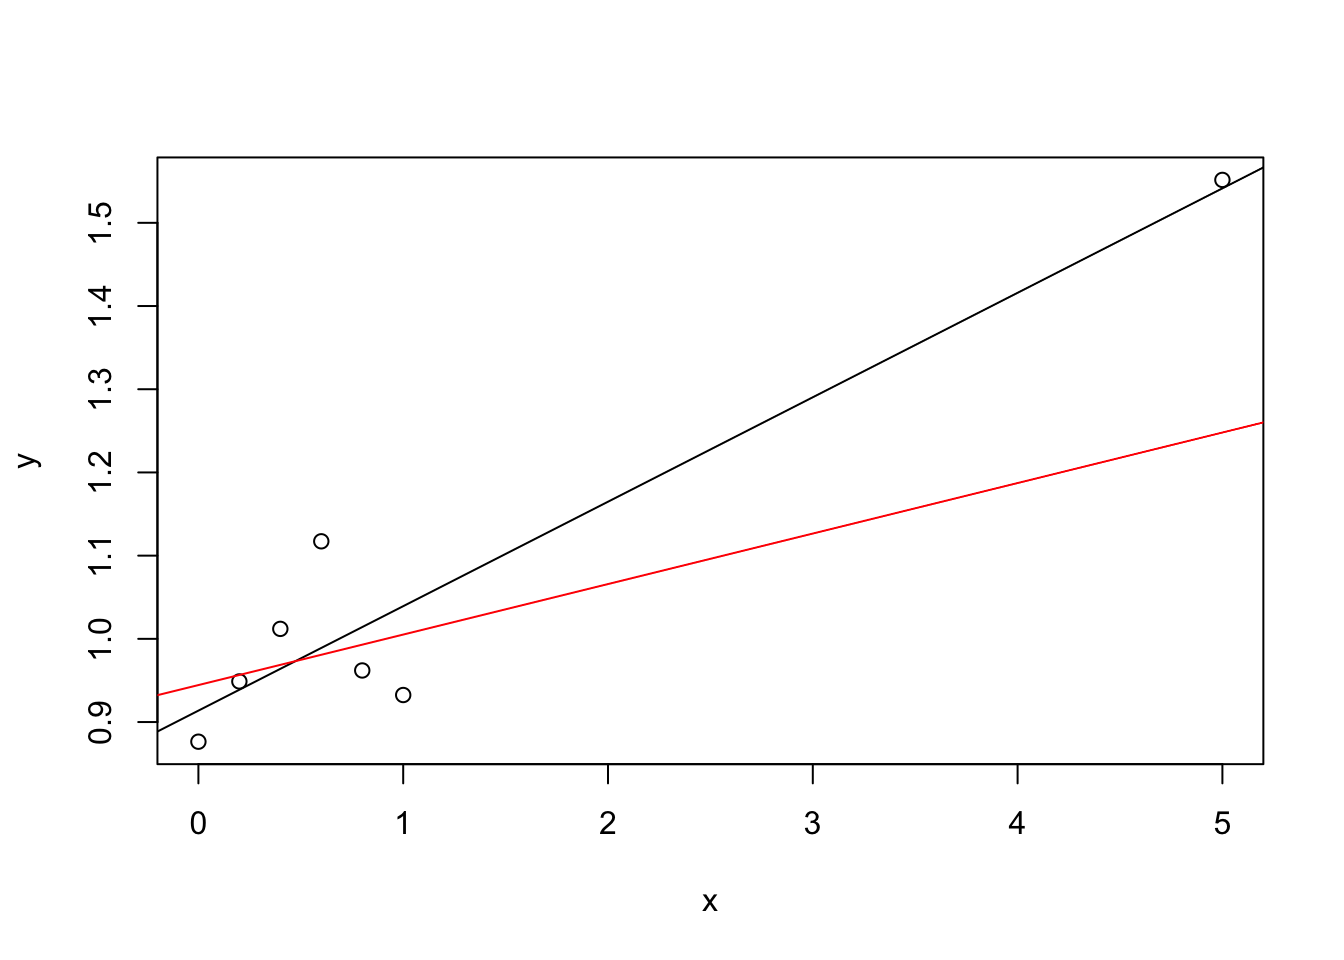
\includegraphics{MATH3714_files/figure-latex/influence-1.pdf}

The black line in the plot is the regression line using all data,
the red line is the regression line fitted using only the left-most
six points and leaving out the ``outlier'' at \(x=5\). The difference
between the two lines makes it clear that the point at \(x=5\) has a
large effect on the estimated regression line. The easiest way
to compute the \(D\)-values seems to be the second formula from
lemma~\ref{lem:Cook-D-alt}:

\begin{Shaded}
\begin{Highlighting}[]
\NormalTok{X }\OtherTok{\textless{}{-}} \FunctionTok{model.matrix}\NormalTok{(m)}
\NormalTok{H }\OtherTok{\textless{}{-}}\NormalTok{ X }\SpecialCharTok{\%*\%} \FunctionTok{solve}\NormalTok{(}\FunctionTok{t}\NormalTok{(X) }\SpecialCharTok{\%*\%}\NormalTok{ X, }\FunctionTok{t}\NormalTok{(X))}
\NormalTok{hii }\OtherTok{\textless{}{-}} \FunctionTok{diag}\NormalTok{(H)}
\NormalTok{D }\OtherTok{\textless{}{-}} \FunctionTok{resid}\NormalTok{(m)}\SpecialCharTok{\^{}}\DecValTok{2} \SpecialCharTok{*}\NormalTok{ hii }\SpecialCharTok{/} \DecValTok{2} \SpecialCharTok{/} \FunctionTok{summary}\NormalTok{(m)}\SpecialCharTok{$}\NormalTok{sigma}\SpecialCharTok{\^{}}\DecValTok{2} \SpecialCharTok{/}\NormalTok{ (}\DecValTok{1} \SpecialCharTok{{-}}\NormalTok{ hii)}\SpecialCharTok{\^{}}\DecValTok{2}
\NormalTok{D}
\end{Highlighting}
\end{Shaded}

\begin{Shaded}
\begin{Highlighting}[]
\NormalTok{\#           1           2           3           4           5           6 }
\NormalTok{\# 6.456405260 0.035318182 0.002129694 0.042504418 0.268374731 0.040765842 }
\NormalTok{\#           7 }
\NormalTok{\# 0.162580015}
\end{Highlighting}
\end{Shaded}

The results show as expected a very large value for the first observation,
\(D_1 = 6.456\), and small values for the remaining \(D_i\).
We can also find Cook's \(D\)-values in the output of the
\texttt{influence.measures()} function:

\begin{Shaded}
\begin{Highlighting}[]
\FunctionTok{influence.measures}\NormalTok{(m)}
\end{Highlighting}
\end{Shaded}

\begin{Shaded}
\begin{Highlighting}[]
\NormalTok{\# Influence measures of}
\NormalTok{\#    lm(formula = y \textasciitilde{} x) :}
\NormalTok{\# }
\NormalTok{\#    dfb.1\_   dfb.x   dffit  cov.r  cook.d   hat inf}
\NormalTok{\# 1 {-}0.7475  3.1083  3.3670 39.046 6.45641 0.967   *}
\NormalTok{\# 2 {-}0.2441  0.1415 {-}0.2441  1.791 0.03532 0.215    }
\NormalTok{\# 3  0.0583 {-}0.0296  0.0585  1.920 0.00213 0.192    }
\NormalTok{\# 4  0.2674 {-}0.1142  0.2720  1.596 0.04250 0.173    }
\NormalTok{\# 5  0.9536 {-}0.3189  0.9959  0.348 0.26837 0.159    }
\NormalTok{\# 6 {-}0.2461  0.0560 {-}0.2681  1.512 0.04077 0.149    }
\NormalTok{\# 7 {-}0.5620  0.0577 {-}0.6512  0.687 0.16258 0.144}
\end{Highlighting}
\end{Shaded}

The table also shows the diagonal elements of the hat matrix, in the
column \texttt{hat}, and some additional measures which we will not discuss here.
A star in the last column, titled \texttt{inf}, marks influential observations.
The star is placed if \emph{any} of the measures shown in the table is significantly
large.
\end{example}

\textbf{Summary}

\begin{itemize}
\tightlist
\item
  We can measure the influence of an observation by the amount
  the estimated parameters change when the observation is deleted.
\item
  We learned how to determine the amount of change without
  having to fit \(n\) additional models.
\item
  Cook's distance provides a numerical measure for the influence of each
  observation.
\end{itemize}

\clearpage

\hypertarget{S10-multicoll}{%
\section{Multicollinearity}\label{S10-multicoll}}

\begin{definition}
In linear regression, \textbf{Multicollinearity} denotes the situation
when the columns of the design matrix \(X\) are (approximately) linearly
dependent.
\end{definition}

The columns of \(X\) are linearly dependent, if and only if
there is a \(v \in \mathbb{R}^{p+1}\) such that \(X v = 0\). The columns
are approximately linearly dependent, if there is a vector \(v\)
such that \(X v \approx 0\).

\hypertarget{consequences-of-multicollinearity}{%
\subsection{Consequences of Multicollinearity}\label{consequences-of-multicollinearity}}

In the derivation of the least squares estimator \(\hat\beta = (X^\top X)^{-1} X^\top y\) we had to assume that the matrix \(X^\top X\) is
invertible. If the columns of \(X\) are linearly dependent, \(X^\top X\) is no
longer invertible and the least squares estimate is no longer uniquely
defined.

\begin{example}
Consider the following data:

\begin{longtable}[]{@{}rcl@{}}
\toprule
\(y\) & \(x_1\) & \(x_2\) \\
\midrule
\endhead
2 & 1 & 1 \\
4 & 2 & 2 \\
6 & 3 & 3 \\
\bottomrule
\end{longtable}

In this case, an exact match with no residuals can be achieved
as \(y = x_1 + x_2\), \emph{i.e.}~for \(\beta_1 = \beta_2 = 1\). But this solution
is not unique: we could just as well write \(y = 2 x_1\) or \(y = 2 x_2\).
Any choice of \(\beta_1\) and \(\beta_2\) with \(\beta_1 + \beta_2 = 2\) will
lead to zero residuals.
\end{example}

The problem in the example above occurs, since the two input columns in the
data are identical. The same problem, in a less obvious way, would occur in
datasets with more inputs when one column of \(X\) can be written as a linear
combination of other columns. This is a problem of the given
input data, not of the responsees or of the statistical model.

In the case where there is only approximate linear dependency between the
columns of \(X\), the inverse \((X^\top X)^{-1}\) exists and an estimate \(\hat\beta\)
can be computed, but there will be huge uncertainties in some of the stimated
coefficients. We illustrate this effect using a numerical example.

\begin{example}
\protect\hypertarget{exm:mulcollell}{}\label{exm:mulcollell}Here we simulate data which has similar characteristics to the toy
example above: we have two inputs, each of which equals the
output with a small amount of noise added. We
fit a model without the intercept, so that there are only two
coefficients to estimate and plotting these is no problem.

\begin{Shaded}
\begin{Highlighting}[]
\FunctionTok{set.seed}\NormalTok{(}\DecValTok{20211101}\NormalTok{)}
\NormalTok{n }\OtherTok{\textless{}{-}} \DecValTok{10}
\NormalTok{y }\OtherTok{\textless{}{-}} \DecValTok{2} \SpecialCharTok{*}\NormalTok{ (}\DecValTok{1}\SpecialCharTok{:}\NormalTok{n)}
\NormalTok{x1 }\OtherTok{\textless{}{-}} \FunctionTok{rnorm}\NormalTok{(}\DecValTok{10}\NormalTok{, }\DecValTok{1}\SpecialCharTok{:}\NormalTok{n, }\FloatTok{0.15}\NormalTok{)}
\NormalTok{x2 }\OtherTok{\textless{}{-}} \FunctionTok{rnorm}\NormalTok{(}\DecValTok{10}\NormalTok{, }\DecValTok{1}\SpecialCharTok{:}\NormalTok{n, }\FloatTok{0.15}\NormalTok{)}
\NormalTok{m }\OtherTok{\textless{}{-}} \FunctionTok{lm}\NormalTok{(y }\SpecialCharTok{\textasciitilde{}} \DecValTok{0} \SpecialCharTok{+}\NormalTok{ x1 }\SpecialCharTok{+}\NormalTok{ x2)}
\end{Highlighting}
\end{Shaded}

Similar to the approach in \protect\hyperlink{coordinates-of-the-outline}{section~6},
we can plot a confidence ellipse. (Don't worry about the details of the
commands used to plot the ellipse.)

\begin{Shaded}
\begin{Highlighting}[]
\NormalTok{sigma.hat }\OtherTok{\textless{}{-}} \FunctionTok{summary}\NormalTok{(m)}\SpecialCharTok{$}\NormalTok{sigma}
\NormalTok{X }\OtherTok{\textless{}{-}} \FunctionTok{model.matrix}\NormalTok{(m)}
\NormalTok{svd }\OtherTok{\textless{}{-}} \FunctionTok{La.svd}\NormalTok{(}\FunctionTok{t}\NormalTok{(X) }\SpecialCharTok{\%*\%}\NormalTok{ X)}
\NormalTok{alpha }\OtherTok{\textless{}{-}} \FloatTok{0.05}
\NormalTok{f.crit }\OtherTok{\textless{}{-}} \FunctionTok{qf}\NormalTok{(}\DecValTok{1} \SpecialCharTok{{-}}\NormalTok{ alpha, }\FunctionTok{ncol}\NormalTok{(X), }\FunctionTok{nrow}\NormalTok{(X) }\SpecialCharTok{{-}} \FunctionTok{ncol}\NormalTok{(X))}
\NormalTok{phi }\OtherTok{\textless{}{-}} \FunctionTok{seq}\NormalTok{(}\DecValTok{0}\NormalTok{, }\DecValTok{2}\SpecialCharTok{*}\NormalTok{pi, }\AttributeTok{length.out =} \DecValTok{201}\NormalTok{)}
\NormalTok{circ }\OtherTok{\textless{}{-}} \FunctionTok{rbind}\NormalTok{(}\FunctionTok{cos}\NormalTok{(phi), }\FunctionTok{sin}\NormalTok{(phi)) }\SpecialCharTok{*} \FunctionTok{sqrt}\NormalTok{(f.crit }\SpecialCharTok{*} \FunctionTok{ncol}\NormalTok{(X) }\SpecialCharTok{*}\NormalTok{ sigma.hat}\SpecialCharTok{\^{}}\DecValTok{2}\NormalTok{)}
\NormalTok{ellipse }\OtherTok{\textless{}{-}}\NormalTok{ svd}\SpecialCharTok{$}\NormalTok{u }\SpecialCharTok{\%*\%}\NormalTok{ (circ }\SpecialCharTok{/} \FunctionTok{sqrt}\NormalTok{(svd}\SpecialCharTok{$}\NormalTok{d)) }\SpecialCharTok{+} \FunctionTok{coef}\NormalTok{(m)}

\FunctionTok{plot}\NormalTok{(ellipse[}\DecValTok{1}\NormalTok{,], ellipse[}\DecValTok{2}\NormalTok{,], }\AttributeTok{type =} \StringTok{"l"}\NormalTok{, }\AttributeTok{asp =} \DecValTok{1}\NormalTok{,}
     \AttributeTok{xlab =} \FunctionTok{expression}\NormalTok{(beta[}\DecValTok{1}\NormalTok{]),}
     \AttributeTok{ylab =} \FunctionTok{expression}\NormalTok{(beta[}\DecValTok{2}\NormalTok{]))}
\FunctionTok{abline}\NormalTok{(}\DecValTok{2}\NormalTok{, }\SpecialCharTok{{-}}\DecValTok{1}\NormalTok{, }\AttributeTok{lty =} \StringTok{"dashed"}\NormalTok{, }\AttributeTok{col =} \StringTok{"blue"}\NormalTok{)}
\FunctionTok{abline}\NormalTok{(}\AttributeTok{v =} \FunctionTok{coef}\NormalTok{(m)[}\DecValTok{1}\NormalTok{], }\AttributeTok{lty =} \StringTok{"dotted"}\NormalTok{)}
\FunctionTok{abline}\NormalTok{(}\AttributeTok{h =} \FunctionTok{coef}\NormalTok{(m)[}\DecValTok{2}\NormalTok{], }\AttributeTok{lty =} \StringTok{"dotted"}\NormalTok{)}
\end{Highlighting}
\end{Shaded}

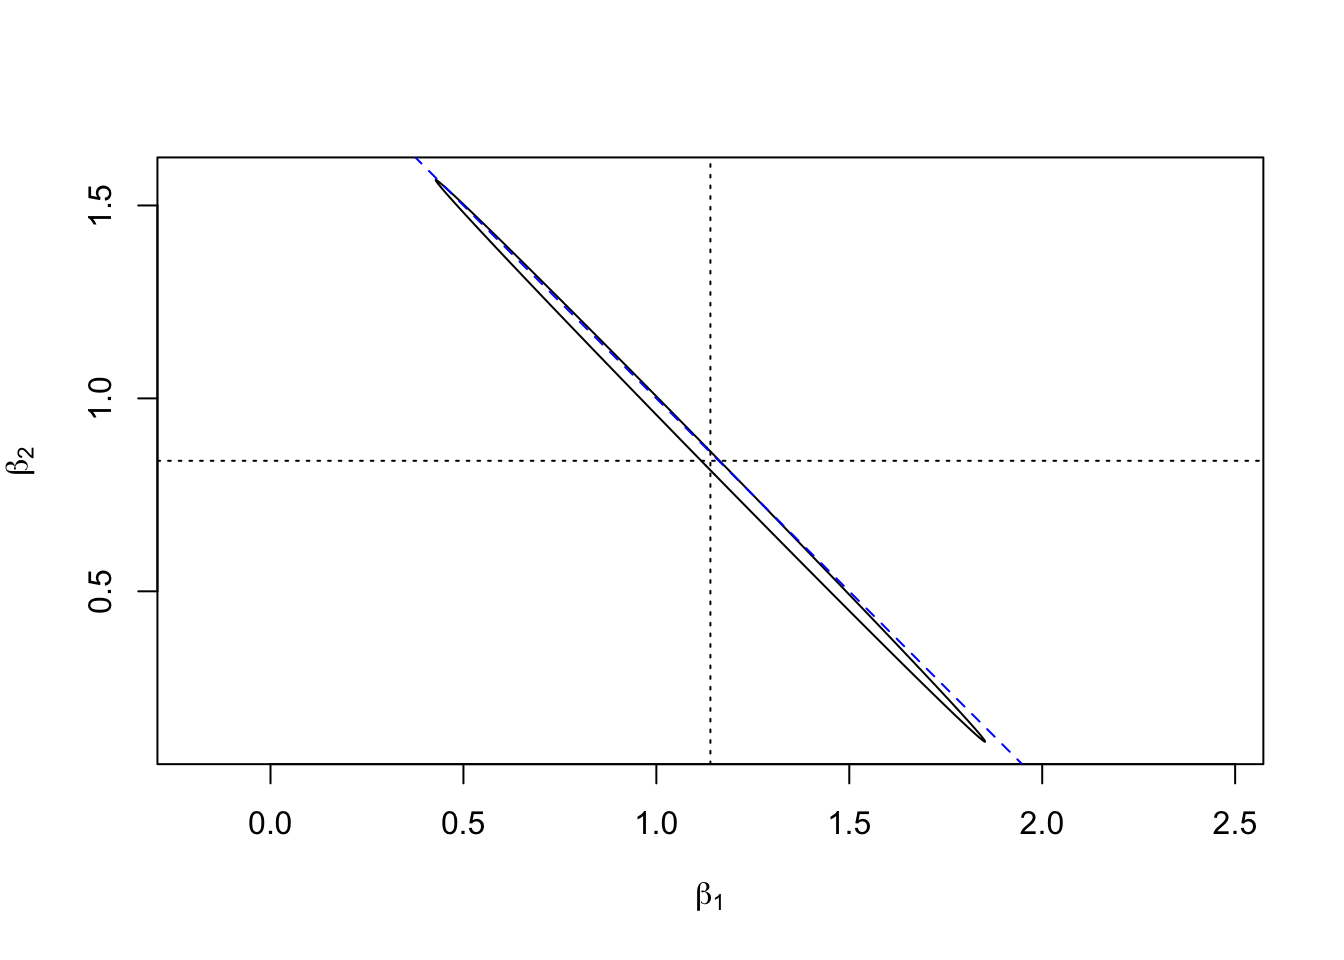
\includegraphics{MATH3714_files/figure-latex/multicollellipse-1.pdf}

We can see that, as in the toy example above, the confidence region
places \((\beta_1, \beta_2)\) close to the line where \(\beta_1 + \beta_2 = 2\)
(the diagonal dashed line), but there is considerable uncertainty about
where on this line the coefficients are located. The effect gets
more pronounced when the amount of noise in the definition of \texttt{x1} and~\texttt{x2}
is reduced.
\end{example}

There are two, slightly different effects of multicollinearity:

\begin{enumerate}
\def\labelenumi{\arabic{enumi}.}
\item
  In the case of exact multicollinearity, \(X^\top X\) is not invertible.
  If the columns of \(X\) are approximately linearly dependent, then
  \((X^\top X)^{-1}\) does exist, but small changes of \(X\) lead to large changes
  of \((X^\top X)^{-1}\) and numerical computation of the inverse is
  strongly affected by rounding errors.
\item
  If the columns of \(X\) are approximately linearly dependent,
  the computed value of the estimator \(\hat\beta\) is strongly affected
  by small changes to the system: the noise in the model strongly affects
  \(\hat\beta\) (as demonstrated in example~\ref{exm:mulcollell}, above),
  leaving out a single observation may lead to large changes in \(\hat\beta\)
  and computation of \(\hat\beta\) is sensitive to rounding errors.
\end{enumerate}

While multicollinearity can make the regression coefficients ambiguous,
the outputs \(y\) are not affected. Predictions made using a model
where multicollinearity is present are still reliable.

\hypertarget{detecting-multicollinearity}{%
\subsection{Detecting Multicollinearity}\label{detecting-multicollinearity}}

While collinearity of two columns of \(X\) is easy to spot, for example in
a pair scatter plot of the inputs \(x_i\), multicollinearity which involves
more than two columns can be harder to notice. The condition number of
\(X\) is a quantitative measure of how close \(X\) is to multicollinearity.

\begin{definition}
The \textbf{condition number} of \(X\) is defined to be
\begin{equation*}
  \kappa(X)
  = \frac{\sigma_\mathrm{max}(X)}{\sigma_\mathrm{min}(X)},
\end{equation*}
where \(\sigma_\mathrm{max}(X) = \sqrt{\lambda_\mathrm{max}(X^\top X)}\) is the
largest singular value of \(X\), computed as the square root of the largest
eigenvalue of \(X^\top X\), and similarly \(\sigma_\mathrm{min}(X) = \sqrt{\lambda_\mathrm{min}(X^\top X)}\) is the smallest singular value of \(X\),
computed as the square root of the smallest eigenvalue of \(X^\top X\).
\end{definition}

As a rule of thumb, if \(\kappa(X) < 10\) there are no significant problems
with multicollinearity, and if \(\kappa(X) > 30\) the regression problem
sufferes severe problems with multicollinearity. In the case where the
columns of \(X\) are exactly linearly dependent, we have \(\sigma_\mathrm{min}(X) = 0\) and \(\kappa(X) = \infty\).

In R, the condition number can be computed using the
\href{https://rdrr.io/r/base/kappa.html}{function \texttt{kappa()}}. The function
can either be called as \texttt{kappa(X,\ exact\ =\ TRUE)},
where \texttt{X} is the design matrix,
or as \texttt{kappa(m,\ exact\ =\ TRUE)}
where \texttt{m} is the object returned by \texttt{lm()}. If the optional
argument \texttt{exact\ =\ TRUE} is omitted, only an approximate result
is returned (using a faster algorithm).

\begin{example}
\protect\hypertarget{exm:multicollell}{}\label{exm:multicollell}Consider the following toy dataset:

\begin{Shaded}
\begin{Highlighting}[]
\NormalTok{data}
\end{Highlighting}
\end{Shaded}

\begin{Shaded}
\begin{Highlighting}[]
\NormalTok{\#        y   x.1    x.2    x.3    x.4}
\NormalTok{\# 1   7.37 4.182  0.078  0.008  1.043}
\NormalTok{\# 2   9.86 6.039  1.106 {-}0.009  0.137}
\NormalTok{\# 3  13.44 9.220  0.151 {-}0.158  0.965}
\NormalTok{\# 4  12.95 8.260 {-}0.018  1.133  0.203}
\NormalTok{\# 5  13.05 8.415  1.078  0.057  0.002}
\NormalTok{\# 6  13.17 9.272 {-}0.019  0.062  0.974}
\NormalTok{\# 7   5.28 1.575 {-}0.160  1.031  0.099}
\NormalTok{\# 8   8.18 4.595  0.091  0.014  0.909}
\NormalTok{\# 9   5.13 2.779 {-}0.074  0.923 {-}0.004}
\NormalTok{\# 10  6.80 2.248 {-}0.045  0.182  1.088}
\end{Highlighting}
\end{Shaded}

To inspect these data, we use a pair scatter plot of the input variables,
leaving out the responses in column~1:

\begin{Shaded}
\begin{Highlighting}[]
\FunctionTok{pairs}\NormalTok{(data[,}\SpecialCharTok{{-}}\DecValTok{1}\NormalTok{])}
\end{Highlighting}
\end{Shaded}

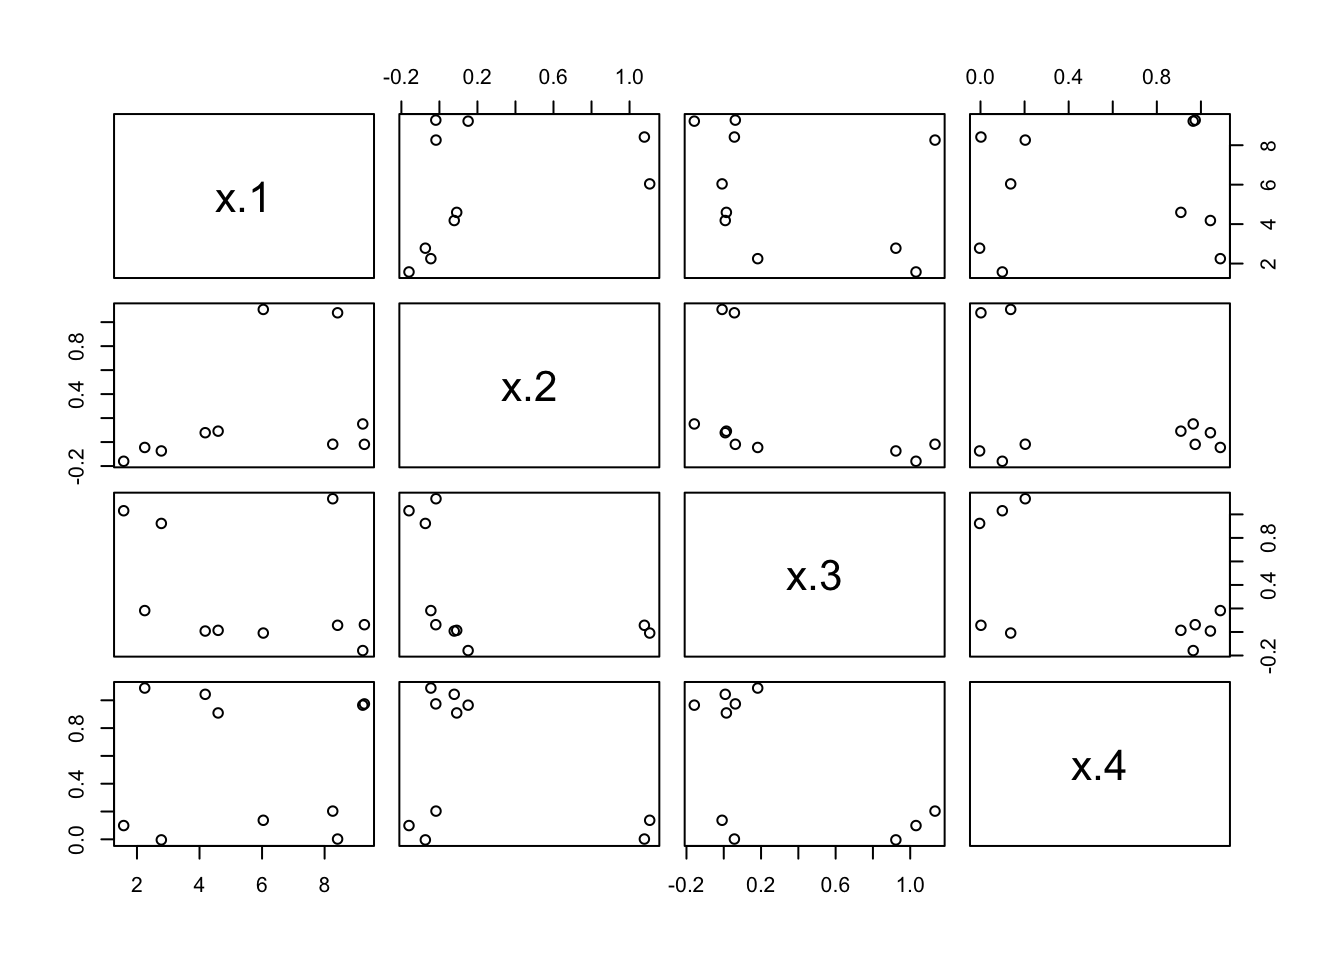
\includegraphics{MATH3714_files/figure-latex/multicollairs-1.pdf}

While there are visbile patterns, there are no clear signs of
a linear dependency between any two columns.
To see whether there are problems with multicollinearity, we fit
a linear model and determine the condition number.

\begin{Shaded}
\begin{Highlighting}[]
\NormalTok{m }\OtherTok{\textless{}{-}} \FunctionTok{lm}\NormalTok{(y }\SpecialCharTok{\textasciitilde{}}\NormalTok{ ., }\AttributeTok{data =}\NormalTok{ data)}
\FunctionTok{kappa}\NormalTok{(m, }\AttributeTok{exact =} \ConstantTok{TRUE}\NormalTok{)}
\end{Highlighting}
\end{Shaded}

\begin{Shaded}
\begin{Highlighting}[]
\NormalTok{\# [1] 97.38214}
\end{Highlighting}
\end{Shaded}

Since the condition number is larger than 30, we can say that the
data shows severe multicollinearity. To find out which variables
are involved, we can use \href{https://en.wikipedia.org/wiki/Singular_value_decomposition}{singular value decomposition}.
This allows to write \(X\) as \(X = U D V^\top\), where \(D\in\mathbb{R}^{(p+1)\times(p+1)}\)
is a diagonal matrix and \(U\in\mathbb{R}^{n\times(p+1)}\) and
\(V\in\mathbb{R}^{(p+1)\times(p+1)}\) are matrices with orthonormal columns.

\begin{Shaded}
\begin{Highlighting}[]
\NormalTok{X }\OtherTok{\textless{}{-}} \FunctionTok{model.matrix}\NormalTok{(m)}
\NormalTok{s }\OtherTok{\textless{}{-}} \FunctionTok{svd}\NormalTok{(X, }\AttributeTok{nu =} \DecValTok{0}\NormalTok{)}
\NormalTok{s}
\end{Highlighting}
\end{Shaded}

\begin{Shaded}
\begin{Highlighting}[]
\NormalTok{\# $d}
\NormalTok{\# [1] 20.3002516  2.0294781  1.8122508  1.2526330  0.2084597}
\NormalTok{\# }
\NormalTok{\# $v}
\NormalTok{\#             [,1]       [,2]        [,3]        [,4]          [,5]}
\NormalTok{\# [1,] {-}0.14024576 {-}0.5552821  0.04218055 {-}0.62161197 {-}0.5327403485}
\NormalTok{\# [2,] {-}0.98554152  0.1088264 {-}0.04131956  0.12311216 {-}0.0009051211}
\NormalTok{\# [3,] {-}0.04170949  0.4036310 {-}0.21603327 {-}0.75981456  0.4597323397}
\NormalTok{\# [4,] {-}0.03395454 {-}0.6495911 {-}0.55665792  0.11926737  0.5027780067}
\NormalTok{\# [5,] {-}0.07839927 {-}0.3081105  0.79998442 {-}0.08306065  0.5020431792}
\end{Highlighting}
\end{Shaded}

We used the optional argument \texttt{nu\ =\ 0} to tell R that we won't need the
matrix~\(U\). The diagonal elements \(\sigma_0(X), \ldots, \sigma_{p}(X) \geq 0\),
stored in \texttt{s\$d}, are the singular values of \(X\) in decreasing order.
We can find the condition number using these values:

\begin{Shaded}
\begin{Highlighting}[]
\NormalTok{s}\SpecialCharTok{$}\NormalTok{d[}\DecValTok{1}\NormalTok{] }\SpecialCharTok{/}\NormalTok{ s}\SpecialCharTok{$}\NormalTok{d[}\FunctionTok{length}\NormalTok{(s}\SpecialCharTok{$}\NormalTok{d)]}
\end{Highlighting}
\end{Shaded}

\begin{Shaded}
\begin{Highlighting}[]
\NormalTok{\# [1] 97.38214}
\end{Highlighting}
\end{Shaded}

This agrees with the value for \(\kappa(X)\) we found above.

Finally, the columns \(v_1, \ldots, v_{p+1}\) of \texttt{s\$v} are called the (right)
singular vectors of \(X\). We can use these vectors to identify which variables
are involved in multicollinearity: It is easy to show that \(\| X v_k \| = \sigma_k(X)\), so every ``small'' \(\sigma_k(X)\) corresponds to a vector \(v_k\)
which describes an approximate linear dependency between the columns of \(X\).
Looking at \(\sigma_4(X)\) (the 5th element of \texttt{s\$d}) we get

\begin{Shaded}
\begin{Highlighting}[]
\FunctionTok{round}\NormalTok{(s}\SpecialCharTok{$}\NormalTok{v[,}\DecValTok{5}\NormalTok{], }\DecValTok{3}\NormalTok{)}
\end{Highlighting}
\end{Shaded}

\begin{Shaded}
\begin{Highlighting}[]
\NormalTok{\# [1] {-}0.533 {-}0.001  0.460  0.503  0.502}
\end{Highlighting}
\end{Shaded}

Rounding the numbers some more and remembering that the first
value corresponds to the intercept, we get that
\begin{equation*}
  -0.5 \cdot 1 + 0.5 \cdot x_2 + 0.5 \cdot x_3 + 0.5 \cdot x_4
  \approx 0
\end{equation*}
or, equivalently
\begin{equation*}
  x_2 + x_3 + x_4
  \approx 1.
\end{equation*}
Looking back over the original numbers we see that this relation
indeed holds.
\end{example}

\hypertarget{mitigations}{%
\subsection{Mitigations}\label{mitigations}}

There are various ways problems resulting from multicollinearity can
be addressed:

\begin{itemize}
\item
  Sometimes columns are lineraly dependent, because a redundant input
  is present. Removing one of the input variables in a group
  of linearly dependent inputs can solve this problem.
\item
  The inputs can be transformed by choosing new variables as functions
  of the original inputs. For example, in example~\ref{exm:multicollell}
  one could try the input variables \(\tilde x_1 = (x_1 + x_2) / 2\) and
  \(\tilde x_2 = (x_1 - x_2) / 2\). The confidence ellipse shown above
  indicates that it should be possible to get good estimates for the
  coefficient for \(\tilde x_1\).
\item
  If \(n\) is small, the problem may be resolved by getting more data.
  In particular, for \(n < p+1\), we \emph{always} have strict multicollinearity.
\item
  Alternative estimation approaches may be used. The basic idea is to sacrifice the
  requirement that \(\hat\beta\) is unbiased, in exchange for a large variance
  reduction. In a later section we will discuss ``ridge regression'' as an
  example of this approach.
\end{itemize}

\textbf{Summary}

\begin{itemize}
\tightlist
\item
  Multicollinearity can lead to numerical problems and large variances in the
  estimated regression coefficients.
\item
  The condition number of the design matrix can be used to detect
  multicollinearity.
\item
  Singular value decomposition can used to better understand linear
  dependencies in the inputs.
\end{itemize}

\clearpage

\hypertarget{P03}{%
\section*{Problem Sheet 3}\label{P03}}
\addcontentsline{toc}{section}{Problem Sheet 3}

You should attempt all these questions and write up your solutions in advance
of your workshop in week~7 where the answers will be discussed.

\textbf{9} Consider the following dataset. Our aim is to predict \(y\) from the
variables \(x_1\), \(x_2\) and \(x_3\).

\begin{longtable}[]{@{}rrrrr@{}}
\toprule
\(i\) & \(x_{1,i}\) & \(x_{2,i}\) & \(x_{3,i}\) & \(y_i\) \\
\midrule
\endhead
1 & -2.17 & -2.08 & -2.16 & 4.47 \\
2 & -1.35 & -0.50 & -0.74 & 5.60 \\
3 & -1.22 & -1.00 & -1.78 & 4.16 \\
4 & -1.04 & -0.32 & -0.40 & 5.52 \\
5 & -0.87 & -0.39 & -0.67 & 5.27 \\
6 & -0.41 & 0.07 & -0.66 & 4.70 \\
7 & 0.07 & 0.74 & 0.37 & 5.50 \\
8 & 0.25 & 0.35 & 0.02 & 4.84 \\
9 & 0.87 & 1.28 & 0.52 & 4.92 \\
10 & 1.53 & 2.30 & 1.35 & 5.35 \\
11 & 2.46 & 2.55 & 1.77 & 4.86 \\
12 & 5.00 & 5.04 & 4.05 & 5.09 \\
\bottomrule
\end{longtable}

These data are also available in machine-readable form at

\begin{itemize}
\tightlist
\item
  \url{http://www1.maths.leeds.ac.uk/~voss/2021/MATH3714/P03Q09.csv}
\end{itemize}

Using these data:

\begin{enumerate}
\def\labelenumi{\alph{enumi}.}
\tightlist
\item
  Fit a linear model of the form
  \(y_i = \beta_0 + x_{1,i} \beta_1 + x_{2,i} \beta_2 + x_{3,i} \beta_3 + \varepsilon_i\).
\end{enumerate}

\begin{myanswers}

To fit the required model we can use the following R commands:

\begin{Shaded}
\begin{Highlighting}[]
\NormalTok{url }\OtherTok{\textless{}{-}} \StringTok{"http://www1.maths.leeds.ac.uk/\textasciitilde{}voss/2021/MATH3714/P03Q09.csv"}
\NormalTok{x }\OtherTok{\textless{}{-}} \FunctionTok{read.csv}\NormalTok{(url)}
\NormalTok{m }\OtherTok{\textless{}{-}} \FunctionTok{lm}\NormalTok{(y }\SpecialCharTok{\textasciitilde{}}\NormalTok{ x1 }\SpecialCharTok{+}\NormalTok{ x2 }\SpecialCharTok{+}\NormalTok{ x3, }\AttributeTok{data=}\NormalTok{x)}
\end{Highlighting}
\end{Shaded}

The fitted model has the following coefficients:

\begin{Shaded}
\begin{Highlighting}[]
\FunctionTok{summary}\NormalTok{(m)}
\end{Highlighting}
\end{Shaded}

\begin{Shaded}
\begin{Highlighting}[]
\NormalTok{\# }
\NormalTok{\# Call:}
\NormalTok{\# lm(formula = y \textasciitilde{} x1 + x2 + x3, data = x)}
\NormalTok{\# }
\NormalTok{\# Residuals:}
\NormalTok{\#       Min        1Q    Median        3Q       Max }
\NormalTok{\# {-}0.104928 {-}0.032723 {-}0.001836  0.024802  0.142993 }
\NormalTok{\# }
\NormalTok{\# Coefficients:}
\NormalTok{\#             Estimate Std. Error t value Pr(\textgreater{}|t|)    }
\NormalTok{\# (Intercept)  4.97725    0.06026  82.598 5.15e{-}13 ***}
\NormalTok{\# x1          {-}1.11954    0.07427 {-}15.074 3.71e{-}07 ***}
\NormalTok{\# x2           0.28176    0.12023   2.344   0.0472 *  }
\NormalTok{\# x3           1.06621    0.09492  11.232 3.54e{-}06 ***}
\NormalTok{\# {-}{-}{-}}
\NormalTok{\# Signif. codes:  0 \textquotesingle{}***\textquotesingle{} 0.001 \textquotesingle{}**\textquotesingle{} 0.01 \textquotesingle{}*\textquotesingle{} 0.05 \textquotesingle{}.\textquotesingle{} 0.1 \textquotesingle{} \textquotesingle{} 1}
\NormalTok{\# }
\NormalTok{\# Residual standard error: 0.07109 on 8 degrees of freedom}
\NormalTok{\# Multiple R{-}squared:  0.9817,  Adjusted R{-}squared:  0.9748 }
\NormalTok{\# F{-}statistic: 142.8 on 3 and 8 DF,  p{-}value: 2.76e{-}07}
\end{Highlighting}
\end{Shaded}

\end{myanswers}

\begin{enumerate}
\def\labelenumi{\alph{enumi}.}
\setcounter{enumi}{1}
\tightlist
\item
  Determine a \(95\%\) confidence interval for the coefficient~\(\beta_2\).
\end{enumerate}

\begin{myanswers}
From lectures we know that a confidence interval for a single
coefficient~\(\beta_j\) is given by
\begin{equation*}
  [U, V]
  = \Bigl[ \hat\beta_j - t_{n-p-1}(\alpha/2) \sqrt{\widehat{\sigma^2} C_{jj}},
       \hat\beta_j + t_{n-p-1}(\alpha/2) \sqrt{\widehat{\sigma^2} C_{jj}} \Bigr],
\end{equation*}
where \(t_{n-p-1}\) is the \((1-\alpha/2)\)-quantile of the \(t\)-distribution,
\(C_{jj} = (X^\top X)^{-1}_{jj}\), and \(X\) is the design matrix.

We can read off the required values for computing the confidence
interval from the output of \texttt{summary(m)}: the centre of the
confidence interval can be found in the column \texttt{Estimate},
the standard error \(\sqrt{\widehat{\sigma^2} C_{jj}}\) is given in
column \texttt{Std.\ Error}, and \(n-p-1 = 12 - 3 - 1 = 8\). Using
these values, we can find a \(95\%\)-confidence interval for
\(\beta_2\) as follows:

\begin{Shaded}
\begin{Highlighting}[]
  \FunctionTok{c}\NormalTok{(}\FloatTok{0.28176} \SpecialCharTok{{-}} \FunctionTok{qt}\NormalTok{(}\FloatTok{0.975}\NormalTok{, }\DecValTok{8}\NormalTok{) }\SpecialCharTok{*} \FloatTok{0.12023}\NormalTok{, }\FloatTok{0.28176} \SpecialCharTok{+} \FunctionTok{qt}\NormalTok{(}\FloatTok{0.975}\NormalTok{, }\DecValTok{8}\NormalTok{) }\SpecialCharTok{*} \FloatTok{0.12023}\NormalTok{)}
\end{Highlighting}
\end{Shaded}

\begin{Shaded}
\begin{Highlighting}[]
\NormalTok{\# [1] 0.004509123 0.559010877}
\end{Highlighting}
\end{Shaded}

Thus, the confidence interval is \(\bigl[ 0.0045, 0.5590 \bigr]\).

\end{myanswers}

\begin{enumerate}
\def\labelenumi{\alph{enumi}.}
\setcounter{enumi}{2}
\tightlist
\item
  Perform a hypothesis test, at the \(95\%\)-level, for the
  hypothesis \(H_0\colon \beta_2 = 0\) with alternative \(H_1\colon \beta_2 \neq 0\).
\end{enumerate}

\begin{myanswers}
The test statistic is
\begin{equation*}
  T
  = \frac{\bigl|\hat\beta_2\bigr|}{\sqrt{\widehat{\sigma^2} C_{jj}} }
  = \frac{0.28176}{0.12023}
  = 2.344.
\end{equation*}
(This value is also shown in the column \texttt{t\ value} of the R
summary output.) The critical value is
\begin{equation*}
  t
  = t_{n-p-1}(\alpha/2)
  = 2.306.
\end{equation*}
Since \(T > t\), we can reject the hypothesis \(\beta_2 = 0\) at the
\(95\%\)-level.

\end{myanswers}

\textbf{10} Let \(x_1, \ldots, x_n, y_1, \ldots, y_n \in \mathbb{R}\) be given. Assume
that it is known that the \(y\)-values satisfy
\(y \approx 1 - x + c x^2 - d x^3\), where \(c\) and \(d\) are unknown
constants.

\begin{enumerate}
\def\labelenumi{\alph{enumi}.}
\tightlist
\item
  Explain how linear regression can be used to estimate the
  parameters \(c\) and \(d\) from the given data.
\end{enumerate}

\begin{myanswers}
We can rewrite the equation for \(y\) as
\begin{equation*}
  y + x - 1 = c x^2 - d x^3,
\end{equation*}
where \(c\) and \(d\) are the unknown quantities, and \(x\) and \(y\)
are given. Thus we can estimate \(c\) and \(d\) by fitting
a linear model with two inputs, \(x_i^2\) and \(x_i^3\)
and one output \(y_i + x_i - 1\). The model does not include
an intercept.

\end{myanswers}

\begin{enumerate}
\def\labelenumi{\alph{enumi}.}
\setcounter{enumi}{1}
\tightlist
\item
  What is the design matrix in this situation?
\end{enumerate}

\begin{myanswers}
Since there is no intercept, the design matrix is
\begin{equation*}
  X = \begin{pmatrix}
    x_1^2 & x_1^3 \\
    x_2^2 & x_2^3 \\
    \vdots & \vdots \\
    x_n^2 & x_n^3 \\
  \end{pmatrix}
  \in \mathbb{R}^{n\times 2}.
\end{equation*}

\end{myanswers}

\begin{enumerate}
\def\labelenumi{\alph{enumi}.}
\setcounter{enumi}{2}
\tightlist
\item
  Why can \emph{linear} regression be used, despite the presence
  of the \emph{non-linear} terms \(x^2\) and~\(x^3\)?
\end{enumerate}

\begin{myanswers}
A linear model is appropriate, because the response depends
on the unknown coefficients \(c\) and \(d\) in a linear way: \(c\) and \(d\)
are only multiplied by known constants, and there are no non-linear
functions of \(c\) and \(d\) in the model.

\end{myanswers}

\textbf{11} In this question we consider four different datasets, given by
inputs \(x_i\) and responses \(y_i\) for \(i \in \{1, 2, 3, 4\}\).

\begin{enumerate}
\def\labelenumi{\alph{enumi}.}
\tightlist
\item
  Based on the following plots, discuss model fit of each model.
  Describe all relevant features of the plots.
  Describe any problems with the model fit you find.
\end{enumerate}

\begin{Shaded}
\begin{Highlighting}[]
    \FunctionTok{par}\NormalTok{(}\AttributeTok{mfrow=}\FunctionTok{c}\NormalTok{(}\DecValTok{4}\NormalTok{,}\DecValTok{2}\NormalTok{))}

\NormalTok{    m1 }\OtherTok{\textless{}{-}} \FunctionTok{lm}\NormalTok{(y1 }\SpecialCharTok{\textasciitilde{}}\NormalTok{ x1)}
    \FunctionTok{plot}\NormalTok{(}\FunctionTok{fitted}\NormalTok{(m1), }\FunctionTok{resid}\NormalTok{(m1), }\AttributeTok{xlab=}\StringTok{"fitted values"}\NormalTok{, }\AttributeTok{ylab=}\StringTok{"residuals"}\NormalTok{)}
    \FunctionTok{qqnorm}\NormalTok{(}\FunctionTok{resid}\NormalTok{(m1), }\AttributeTok{main=}\ConstantTok{NULL}\NormalTok{)}

\NormalTok{    m2 }\OtherTok{\textless{}{-}} \FunctionTok{lm}\NormalTok{(y2 }\SpecialCharTok{\textasciitilde{}}\NormalTok{ x2)}
    \FunctionTok{plot}\NormalTok{(}\FunctionTok{fitted}\NormalTok{(m2), }\FunctionTok{resid}\NormalTok{(m2), }\AttributeTok{xlab=}\StringTok{"fitted values"}\NormalTok{, }\AttributeTok{ylab=}\StringTok{"residuals"}\NormalTok{)}
    \FunctionTok{qqnorm}\NormalTok{(}\FunctionTok{resid}\NormalTok{(m2), }\AttributeTok{main=}\ConstantTok{NULL}\NormalTok{)}

\NormalTok{    m3 }\OtherTok{\textless{}{-}} \FunctionTok{lm}\NormalTok{(y3 }\SpecialCharTok{\textasciitilde{}}\NormalTok{ x3)}
    \FunctionTok{plot}\NormalTok{(}\FunctionTok{fitted}\NormalTok{(m3), }\FunctionTok{resid}\NormalTok{(m3), }\AttributeTok{xlab=}\StringTok{"fitted values"}\NormalTok{, }\AttributeTok{ylab=}\StringTok{"residuals"}\NormalTok{)}
    \FunctionTok{qqnorm}\NormalTok{(}\FunctionTok{resid}\NormalTok{(m3), }\AttributeTok{main=}\ConstantTok{NULL}\NormalTok{)}

\NormalTok{    m4 }\OtherTok{\textless{}{-}} \FunctionTok{lm}\NormalTok{(y4 }\SpecialCharTok{\textasciitilde{}}\NormalTok{ x4)}
    \FunctionTok{plot}\NormalTok{(}\FunctionTok{fitted}\NormalTok{(m4), }\FunctionTok{resid}\NormalTok{(m4), }\AttributeTok{xlab=}\StringTok{"fitted values"}\NormalTok{, }\AttributeTok{ylab=}\StringTok{"residuals"}\NormalTok{)}
    \FunctionTok{qqnorm}\NormalTok{(}\FunctionTok{resid}\NormalTok{(m4), }\AttributeTok{main=}\ConstantTok{NULL}\NormalTok{)}
\end{Highlighting}
\end{Shaded}

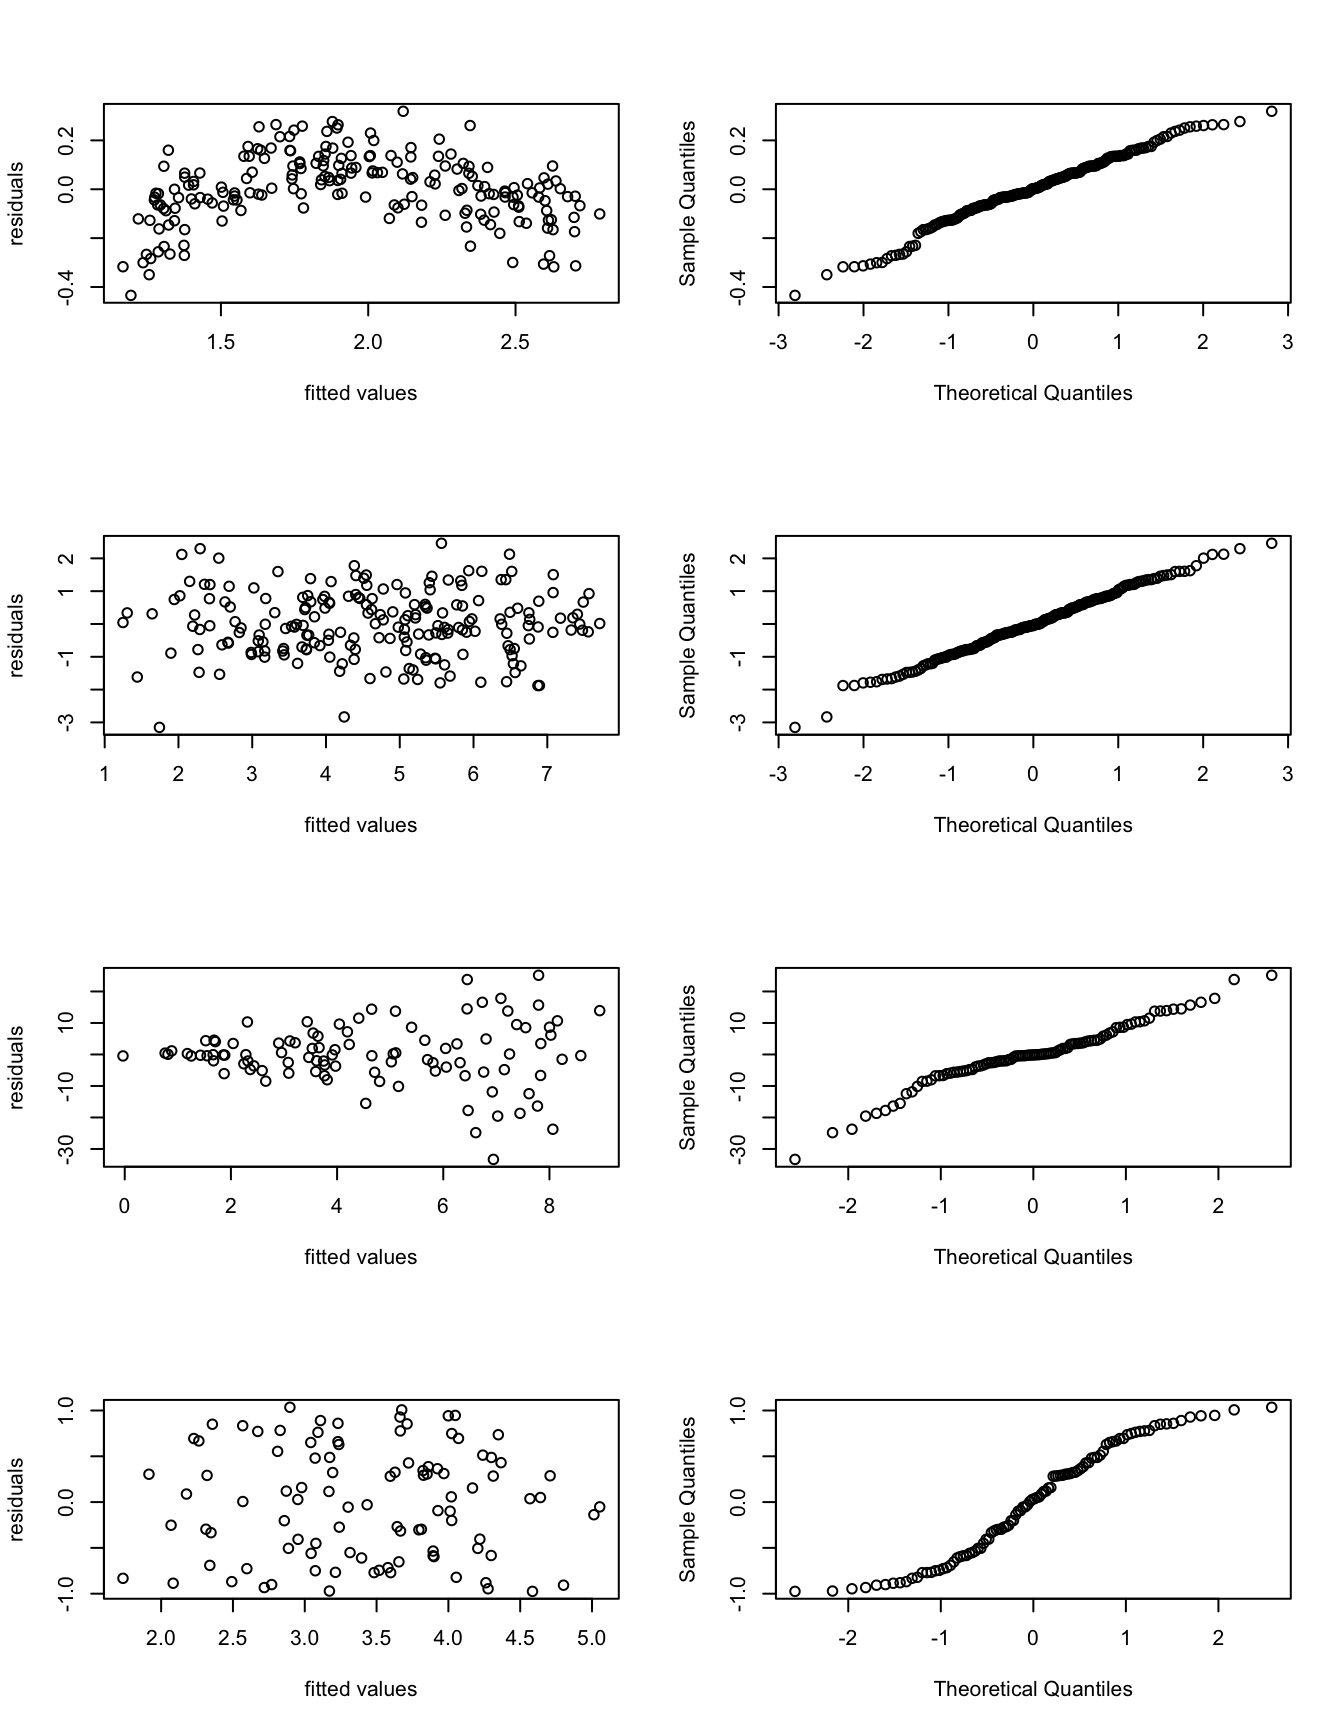
\includegraphics{MATH3714_files/figure-latex/four-models-1.pdf}

\begin{myanswers}

We first note that the given R commands generate the plots along
rows, so the first row of plots corresponds to model~\texttt{m1}, the
second row to model~\texttt{m2}, and so on. The plots shown are
residual plots in the left column, and Q-Q-plots in the right
column.

\begin{itemize}
\tightlist
\item
  \textbf{m1:} Samples in the residual plot on the left
  seem to follow an upside down parabola indicating a non-linear
  relationship between \(x\) and \(y\). Samples in the QQ-plot on the
  right seem to (approximately?) follow a straight line, so
  residuals seem to be (approximately?) normally distributed. No
  outliers are visible.
\item
  \textbf{m2:} Samples in the residual plot form a band
  centred at zero. Possibly very negative residuals are less
  frequent for fitted values \(\hat y_i < 4\)? No outliers are
  apparent. The samples in the QQ-plot seem to clearly fall on a
  straight line. Overall, model fit seems very good.
\item
  \textbf{m3:} The samples in the residual plot are
  centred around \(\hat\varepsilon= 0\), but the width of the spread
  increases as the fitted values increase, leasing to a triangular
  shape. This indicates that the variance of the residuals is not
  constant but increases with \(y\). Possibly, a model with
  multiplicative noise would be appropriate for these data. The
  QQ-plot shows an approximately straight line, but fit is not as
  good as for model~\texttt{m2}.
\item
  \textbf{m4:} The samples in the residual plot form a
  horizontal band centred at~\(\hat\varepsilon= 0\), no outliers are
  visible. The QQ-plot shows clearly that the residuals are not
  normally distributed: the samples form an ``S-shaped'' line,
  indicating that the errors have lighter tails than we would expect
  for a normal distribution.
\end{itemize}

\end{myanswers}

\begin{enumerate}
\def\labelenumi{\alph{enumi}.}
\setcounter{enumi}{1}
\tightlist
\item
  Which of the four models has the best fit?
\end{enumerate}

\begin{myanswers}
The data in \texttt{m1} seems to
have a non-linear relationship between \(x\) and~\(y\), the data
in~\texttt{m3} seems to be better modelled using multiplicative noise,
and the residuals in~\texttt{m4} seem not to be normally
distributed. Thus, the model with the best fit is~\texttt{m2},
because it is the only model which does not show any obvious
problems.

\end{myanswers}

\textbf{12} Using singular value decomposition,
we can write a design matrix \(X\) as \(X = U D V^\top\),
where \(D\in\mathbb{R}^{(p+1)\times(p+1)}\) is a diagonal matrix
and \(U\in\mathbb{R}^{n\times(p+1)}\) and \(V\in\mathbb{R}^{(p+1)\times(p+1)}\) are matrices with orthonormal columns.
Denote the diagonal elements of \(D\) by \(\sigma_0(X), \ldots, \sigma_p(X) \geq 0\),
and the columns of \(V\) by \(v_0, \ldots, v_p\).
Show that \(\| X v_k \| = \sigma_k(X)\).
(We used this fact in example~\ref{exm:multicollell}.)

\begin{myanswers}
Using the singular value decomposition of \(X\), we find
\begin{equation*}
  \| X v_k \|
  = \| U D V^\top v_k \|.
\end{equation*}
For every vector \(x\) we
have \(\| U x \|^2 = x^\top U^\top U x = x^\top x = \| x \|^2\).
Thus, multiplying a vector \(x\) by \(U\) does
not change its length. Using this rule we find
\begin{equation*}
  \| X v_k \|
  = \| D V^\top v_k \|.
\end{equation*}
Since the columns of \(V\) are orthonormal, we have \(V^\top v_k = e_k\),
where \(e_k = (0, \ldots, 1, \ldots, 0)\) is the \(k\)th standard basis vector.
Thus we get
\begin{equation*}
  \| X v_k \|
  = \| D e_k \|
  = \| \sigma_k(X) e_k \|
  = \sigma_k(X) \| e_k \|
  = \sigma_k(X)
\end{equation*}
as required. This completes the proof.

\end{myanswers}

\clearpage

\hypertarget{S11-improving}{%
\section{Improving the Model Fit}\label{S11-improving}}

When we developed the theory for linear models, we used the following
assumptions:

\begin{itemize}
\item
  Linear relationship between inputs and outputs: \(y \approx x^\top \beta\)
\item
  Independence of errors: the \(\varepsilon_i = y_i - x_i^\top\beta\) are independent
  of each other.
\item
  Normally distributed errors: \(\varepsilon_i \sim \mathcal{N}(0, \sigma^2)\) for all \(i\).
  In particular, the variance of the \(\varepsilon_i\) does not depend on~\(i\).
\end{itemize}

The \protect\hyperlink{plots}{diagnostic plots} mentioned in section~\ref{plots}
can often reveal if the data do not fit these modelling assumptions.
In cases where
the assumptions are violated, sometimes a linear model can still
be used if the data is transformed first.

\hypertarget{linearising-the-mean}{%
\subsection{Linearising the Mean}\label{linearising-the-mean}}

If the model mean is a non-linear function of the inputs, we
can sometimes transform the variables to achieve a linear relationship.
We list some examples of non-linear models which can be transformed
to linear models:

\begin{longtable}[]{@{}
  >{\raggedright\arraybackslash}p{(\columnwidth - 4\tabcolsep) * \real{0.5195}}
  >{\raggedright\arraybackslash}p{(\columnwidth - 4\tabcolsep) * \real{0.2597}}
  >{\raggedright\arraybackslash}p{(\columnwidth - 4\tabcolsep) * \real{0.2208}}@{}}
\toprule
\begin{minipage}[b]{\linewidth}\raggedright
nonlinear model
\end{minipage} & \begin{minipage}[b]{\linewidth}\raggedright
transformation
\end{minipage} & \begin{minipage}[b]{\linewidth}\raggedright
linear Model
\end{minipage} \\
\midrule
\endhead
\(y \approx \beta_0 x^{\beta_1}\) & \(x'=\log(x)\), \(y'=\log(y)\) & \(y' \approx \log(\beta_0) + \beta_1 x'\) \\
\(y \approx \beta_0 e^{\beta_1 x}\) & \(y'=\log y\) & \(y' \approx \log \beta_0 +\beta_1 x\) \\
\(y \approx \beta_0+\beta_1\log x\) & \(x'=\log x\) & \(y \approx \beta_0+\beta_1 x'\) \\
\(y \approx \frac{x}{\beta_0 x-\beta_1}\) & \(x'=1/x\), \(y'=1/y\) & \(y' \approx \beta_0-\beta_1 x'\) \\
\bottomrule
\end{longtable}

In all such cases we also would need to check the residuals of the transformed
models, to see whether linear regression can be used for the transformed model.

\hypertarget{stabilising-the-variance}{%
\subsection{Stabilising the Variance}\label{stabilising-the-variance}}

The assumption of constant variance is a basic requirement of regression
analysis. A common reason for the violation of this assumption is for the
response variable \(y\) to follow a distribution in which the variance depends
on \(y\) or \(\mathbb{E}(y)\) and thus on~\(x\).

\begin{example}
The error in our model
\begin{equation*}
  Y
  = \beta_0 + \beta_1 x_1 + \beta_2 x_2 + \cdots + \beta_p x_p + \varepsilon
  = x^\top \beta + \varepsilon
\end{equation*}
is sometimes called \textbf{additive error}, since it is added to the model
mean~\(x^\top\beta\). Sometimes the error is instead given in percentages of the
quantity of interest. In these cases we speak of \textbf{multiplicative error}.
This can, for example, be modelled as
\begin{equation*}
  Y
  = \bigl(\beta_0 + \beta_1 x_1 + \beta_2 x_2 + \cdots + \beta_p x_p\bigr) \exp(\varepsilon)
  = x^\top \beta \exp(\varepsilon).
\end{equation*}
For \(\varepsilon= 0\) we have \(\exp(0) = 1\) and thus \(Y = x^\top \beta\). Similarly,
for small \(\varepsilon\) we have \(Y \approx x^\top \beta\), but the variance is now
proportional to \((x^\top\beta)^2\) instead of being constant. Also, since the
exponential is nonlinear we only have \(\mathbb{E}(Y) \approx x^\top\beta\) instead of
strict equality.
\end{example}

Some commonly-used variance stabilising transformations are:

\begin{longtable}[]{@{}ll@{}}
\toprule
variance & transformation \\
\midrule
\endhead
\(\sigma^2 = \text{constant}\) & no transformation \\
\(\sigma^2 \propto y\) & \(y' = \sqrt{y}\) \\
\(\sigma^2 \propto y^2\) & \(y' = \log y\) \\
\(\sigma^2 \propto y^3\) & \(y' = \frac{1}{\sqrt{y}}\) \\
\(\sigma^2 \propto y^4\) & \(y' = \frac{1}{y}\) \\
\(\sigma^2 \propto y(1-y)\) where \(y \in [0,1]\) & \(y' = \arcsin(\sqrt{y})\) \\
\bottomrule
\end{longtable}

Of course we do not have accurate knowledge of the relationship, but it can be
diagnosed from the residual plots and transformations can be selected by
experimenting with different choices. Any of these transformations will also
affect the mean and we need to check the model fit for the transformed data, to
see whether the transformed data can still reasonably be described by a linear
model.

\begin{example}
The last transformation in the table above corresponds to the case of binomial
sampling: If \(x = p\) and \(Y \sim B(n, p) / n\) then we have \(\mathbb{E}(Y) = n p / n = x\) and a linear model may be appropriate. But we also have \(\mathop{\mathrm{Var}}(Y) = p (1 - p) / n \propto \mathbb{E}(Y) \bigl( 1- \mathbb{E}(Y) \bigr)\), so the assumption of
constant variance is violated.

We try to apply the transformation suggested in the table. The
function \(\arcsin\) is the inverse of the sine function. In R
this function is available as \texttt{asin()}. To get some intuition about
this transformation, we plot the function \(y \mapsto \arcsin(\sqrt{y})\):

\begin{Shaded}
\begin{Highlighting}[]
\NormalTok{y }\OtherTok{\textless{}{-}} \FunctionTok{seq}\NormalTok{(}\DecValTok{0}\NormalTok{, }\DecValTok{1}\NormalTok{, }\AttributeTok{l=}\DecValTok{101}\NormalTok{)}
\FunctionTok{plot}\NormalTok{(y, }\FunctionTok{asin}\NormalTok{(}\FunctionTok{sqrt}\NormalTok{(y)), }\AttributeTok{type =} \StringTok{"l"}\NormalTok{,}
     \AttributeTok{ylab =} \FunctionTok{expression}\NormalTok{(y }\SpecialCharTok{*}\NormalTok{ minute))}
\end{Highlighting}
\end{Shaded}

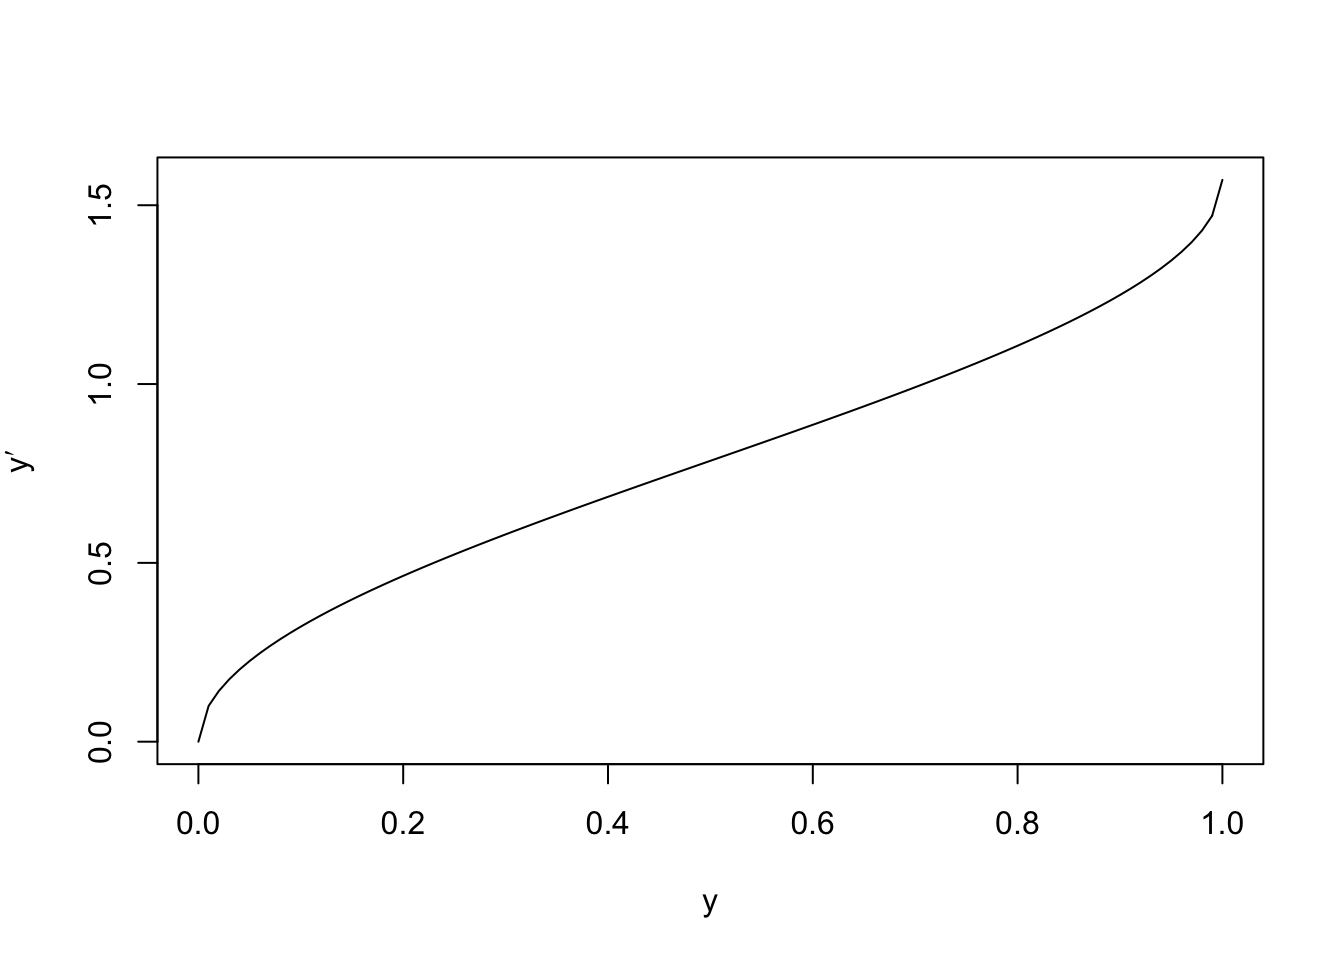
\includegraphics{MATH3714_files/figure-latex/arcsin-transform-1.pdf}

We can see that the transformation is approximately linear for most
of the interval, but has a steeper slope near the edges. The effect of
this is to increase the size of fluctations for small and large
\(y\)-values. We now consider residual plots for the original and transformed
data, for a simulated dataset:

\begin{Shaded}
\begin{Highlighting}[]
\NormalTok{n }\OtherTok{\textless{}{-}} \DecValTok{500}
\NormalTok{x }\OtherTok{\textless{}{-}} \FunctionTok{runif}\NormalTok{(n, }\DecValTok{0}\NormalTok{, }\DecValTok{1}\NormalTok{)}
\NormalTok{y }\OtherTok{\textless{}{-}} \FunctionTok{rbinom}\NormalTok{(n, }\DecValTok{100}\NormalTok{, x) }\SpecialCharTok{/} \DecValTok{100}

\FunctionTok{par}\NormalTok{(}\AttributeTok{mfrow =} \FunctionTok{c}\NormalTok{(}\DecValTok{1}\NormalTok{, }\DecValTok{2}\NormalTok{))}

\NormalTok{m1 }\OtherTok{\textless{}{-}} \FunctionTok{lm}\NormalTok{(y }\SpecialCharTok{\textasciitilde{}}\NormalTok{ x)}
\FunctionTok{plot}\NormalTok{(}\FunctionTok{fitted}\NormalTok{(m1), }\FunctionTok{resid}\NormalTok{(m1))}

\NormalTok{y.prime }\OtherTok{\textless{}{-}} \FunctionTok{asin}\NormalTok{(}\FunctionTok{sqrt}\NormalTok{(y))}
\NormalTok{m2 }\OtherTok{\textless{}{-}} \FunctionTok{lm}\NormalTok{(y.prime }\SpecialCharTok{\textasciitilde{}}\NormalTok{ x)}
\FunctionTok{plot}\NormalTok{(}\FunctionTok{fitted}\NormalTok{(m2), }\FunctionTok{resid}\NormalTok{(m2))}
\end{Highlighting}
\end{Shaded}

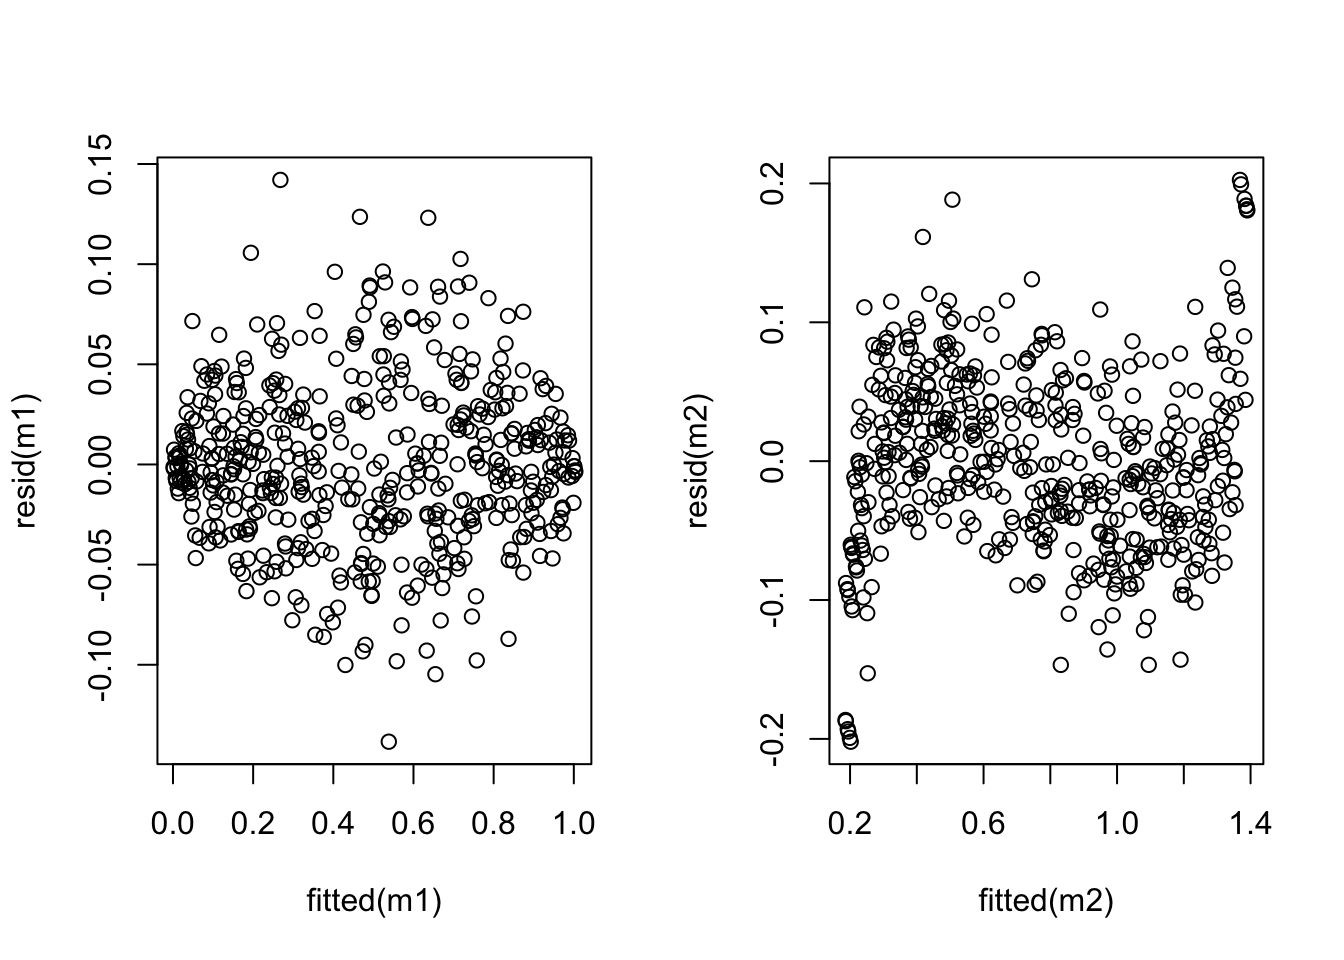
\includegraphics{MATH3714_files/figure-latex/binomial-sampling-1.pdf}

The plot shows that the variance has indeed improved, while linearity
has suffered (an S-shaped curve is now visible). Neither model is perfect and
whether the transformation
is benenficial or not depends on the particular circumstances.
\end{example}

\begin{example}
\protect\hypertarget{exm:electric}{}\label{exm:electric}An electric utility company is interested in developing a model relating the
peak hour demand (\(y\), measured in kW) to total energy usage during the month
(\(x\), in kWh). A scatter plot of the data is shown below:

\begin{Shaded}
\begin{Highlighting}[]
\CommentTok{\# data at https://www1.maths.leeds.ac.uk/\textasciitilde{}voss/2021/MATH3714/electric.dat}
\NormalTok{d }\OtherTok{\textless{}{-}} \FunctionTok{read.table}\NormalTok{(}\StringTok{"data/electric.dat"}\NormalTok{, }\AttributeTok{header=}\ConstantTok{FALSE}\NormalTok{)}
\FunctionTok{plot}\NormalTok{(d}\SpecialCharTok{$}\NormalTok{V1, d}\SpecialCharTok{$}\NormalTok{V2,}
     \AttributeTok{xlab=}\StringTok{"energy usage [kWh]"}\NormalTok{, }\AttributeTok{ylab=}\StringTok{"energy demand [kW]"}\NormalTok{)}
\NormalTok{m1 }\OtherTok{=} \FunctionTok{lm}\NormalTok{(V2 }\SpecialCharTok{\textasciitilde{}}\NormalTok{ ., }\AttributeTok{data =}\NormalTok{ d)}
\FunctionTok{abline}\NormalTok{(m1)}
\end{Highlighting}
\end{Shaded}

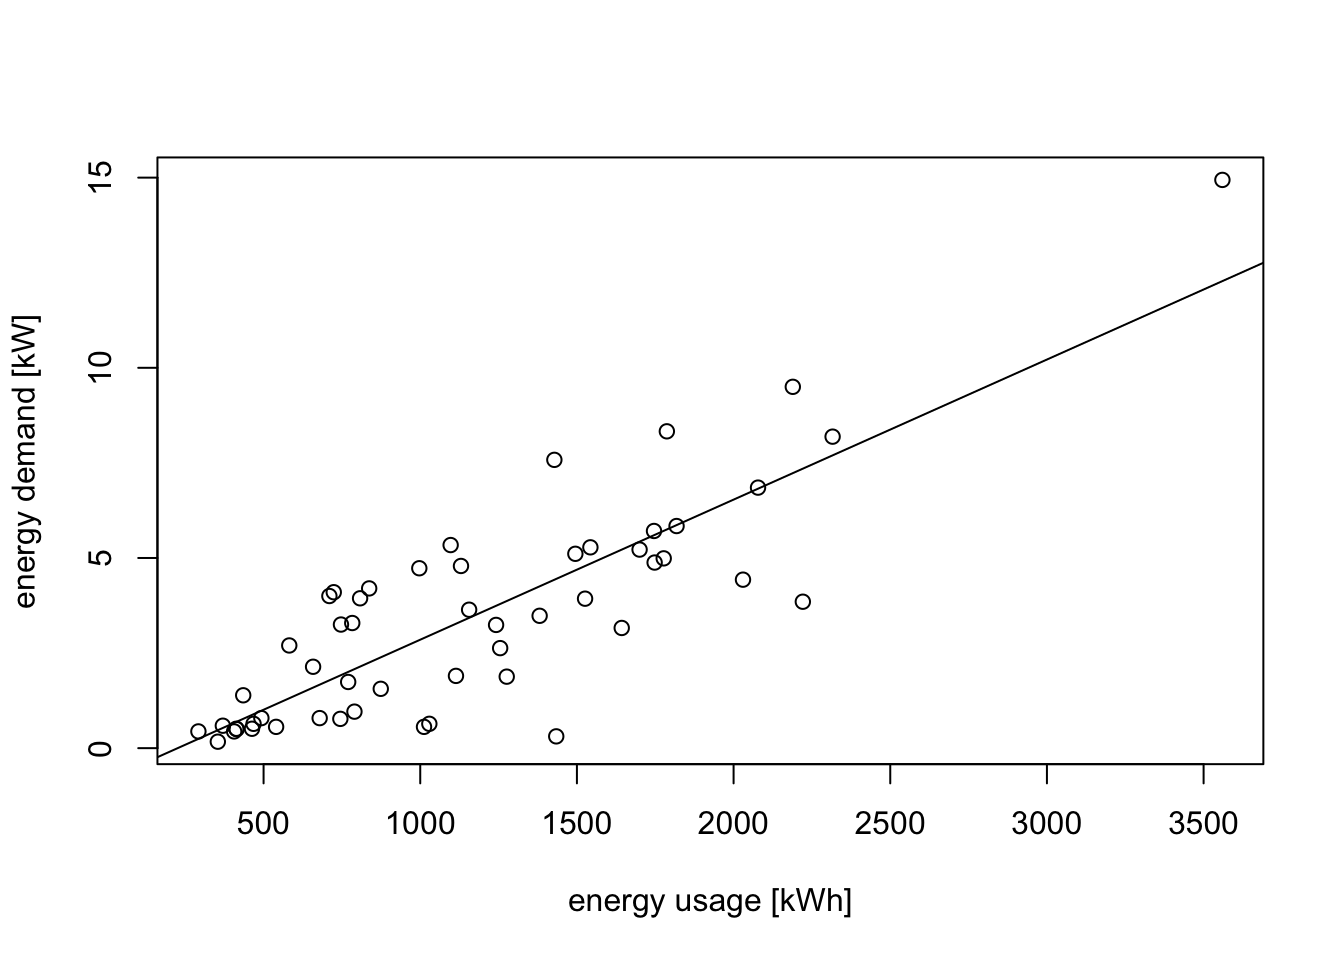
\includegraphics{MATH3714_files/figure-latex/electric1-1.pdf}

A linear relationship looks plausible, but we can see that the spread
of points around the regression line widens as energy usage increases.
this is more clearly visible in a residual plot:

\begin{Shaded}
\begin{Highlighting}[]
\FunctionTok{plot}\NormalTok{(}\FunctionTok{fitted}\NormalTok{(m1), }\FunctionTok{resid}\NormalTok{(m1),}
     \AttributeTok{xlab =} \StringTok{"fitted values"}\NormalTok{, }\AttributeTok{ylab =} \StringTok{"residuals"}\NormalTok{)}
\end{Highlighting}
\end{Shaded}

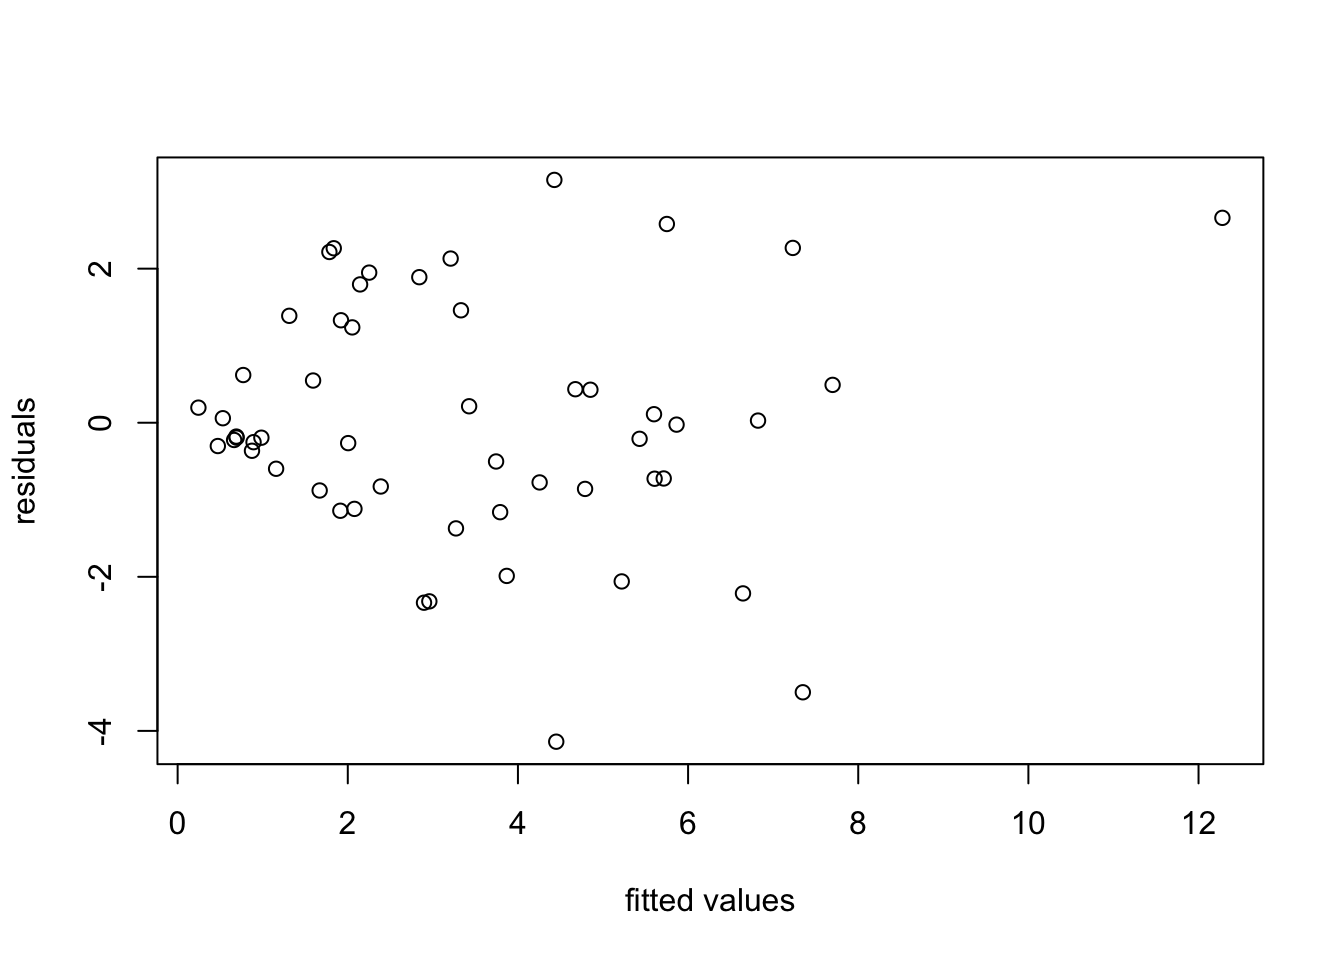
\includegraphics{MATH3714_files/figure-latex/electric2-1.pdf}

We try a transformation of the data to stabilise the variance.
From the ``wedge'' shape on the left hand side of the plot, it is clear
that the variance \(\sigma^2\) increases as \(y\) increases.
Thus we can try transformations like \(y' = \log(y)\) or
\(y' = \sqrt{y}\). Taking the logarithm for illustration, we get

\begin{Shaded}
\begin{Highlighting}[]
\NormalTok{m2 }\OtherTok{\textless{}{-}} \FunctionTok{lm}\NormalTok{(}\FunctionTok{log}\NormalTok{(V2) }\SpecialCharTok{\textasciitilde{}}\NormalTok{ ., }\AttributeTok{data =}\NormalTok{ d)}
\FunctionTok{plot}\NormalTok{(d}\SpecialCharTok{$}\NormalTok{V1, }\FunctionTok{log}\NormalTok{(d}\SpecialCharTok{$}\NormalTok{V2),}
     \AttributeTok{xlab=}\StringTok{"energy usage [kWh]"}\NormalTok{, }\AttributeTok{ylab=}\StringTok{"log{-}transformed y"}\NormalTok{)}
\FunctionTok{abline}\NormalTok{(m2)}
\end{Highlighting}
\end{Shaded}

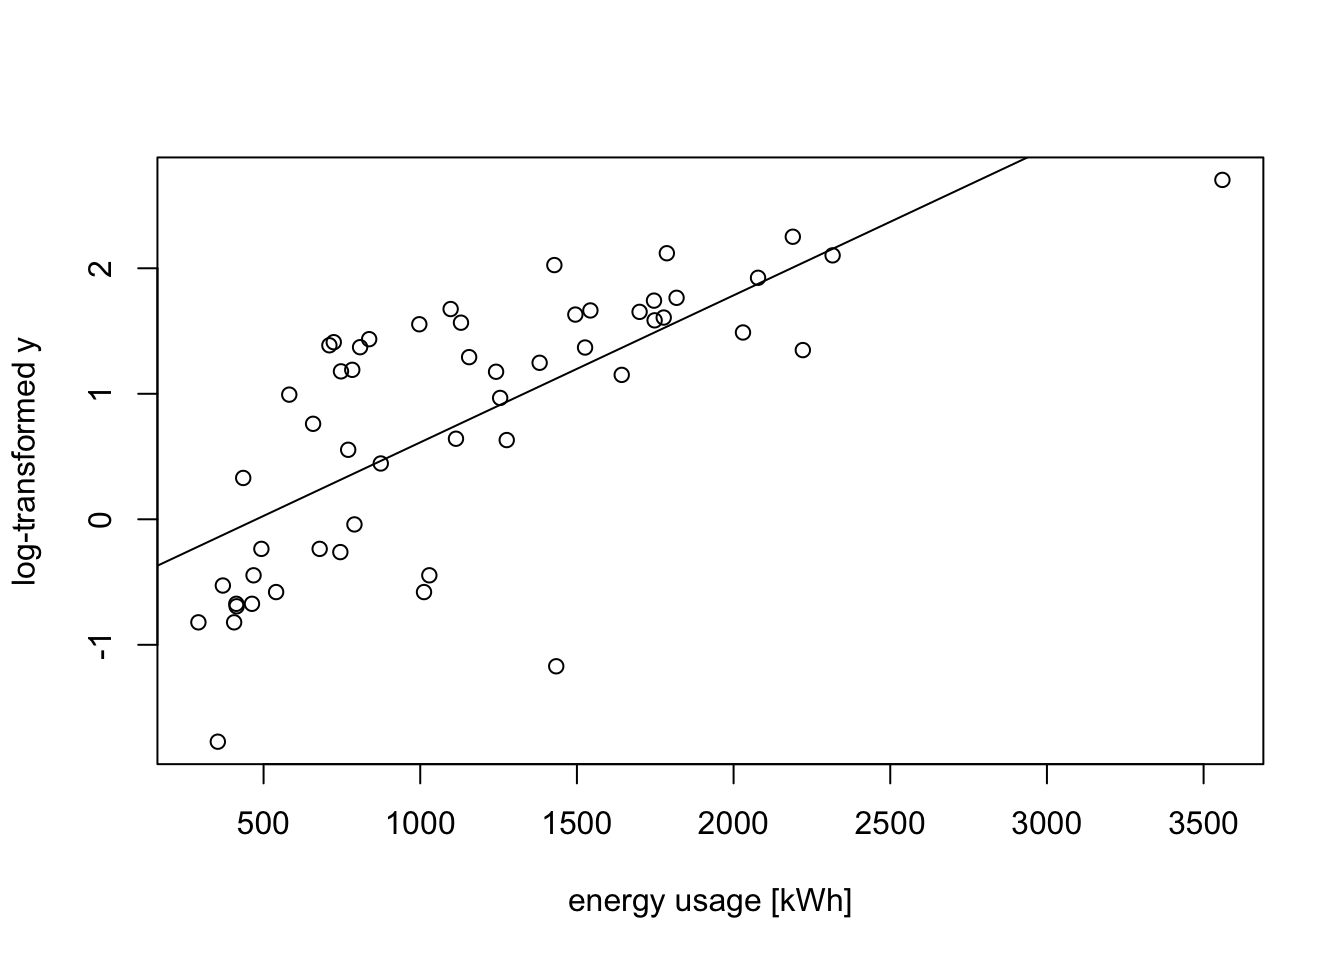
\includegraphics{MATH3714_files/figure-latex/electric3-1.pdf}

\begin{Shaded}
\begin{Highlighting}[]
\FunctionTok{plot}\NormalTok{(}\FunctionTok{fitted}\NormalTok{(m2), }\FunctionTok{resid}\NormalTok{(m2),}
     \AttributeTok{xlab =} \StringTok{"fitted values"}\NormalTok{, }\AttributeTok{ylab =} \StringTok{"residuals for log{-}transform"}\NormalTok{)}
\FunctionTok{abline}\NormalTok{(}\AttributeTok{h =} \DecValTok{0}\NormalTok{)}
\end{Highlighting}
\end{Shaded}

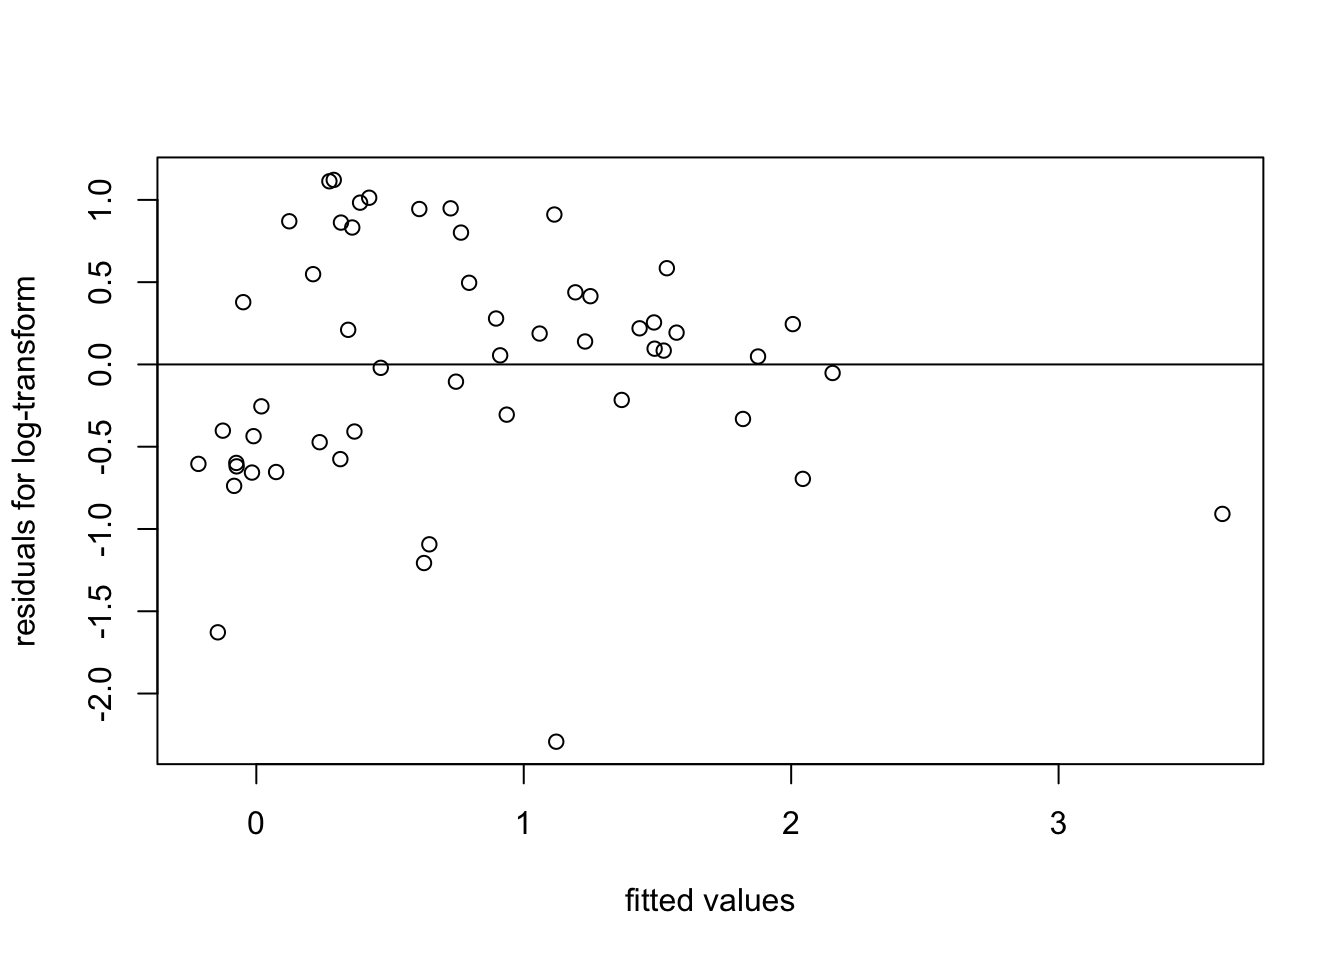
\includegraphics{MATH3714_files/figure-latex/electric4-1.pdf}

The spread of residuals now looks somewhat more reasonable.
\end{example}

\hypertarget{power-transform}{%
\subsection{The Power Transform}\label{power-transform}}

A family of transformations for the response variable \(y\) is given by the
\textbf{power transform}. These transformations only apply to strictly positive data,
\emph{i.e.}~\(y > 0\), and are defined by
\begin{equation*}
  y^{(\lambda)}
  = \begin{cases}
      \frac{\displaystyle y^\lambda-1}{\displaystyle\lambda g^{\lambda-1}} & \mbox{if $\lambda\ne 0$} \\
      g\log y & \mbox{if $\lambda=0$}
    \end{cases}
\end{equation*}
where \(g = (\prod_{i=1}^n y_i)^{1/n}\) is the geometric mean.

The geometric mean is a constant (it does not depend on \(i\)) and is not needed
for the power transform, but it is usually included to make values for
different \(\lambda\) more comparable. For \(\lambda = 1\) the transform is \(y' = y - 1\). This is a simple shift which has no effect on the fitted model, it just
decreases the intercept by \(1\) and leaves the residuals unchanged. Thus, this
case is that same as applying no transformation.

Using Taylor approximation on the numerator in the definition
of~\(y^{(\lambda)}\) we get
\begin{equation*}
  y^\lambda
  = \exp\bigl( \log(y^\lambda) \bigr)
  = \exp\bigl( \lambda \log(y) \bigr)
  \approx 1 + \lambda\log(y) + O\Bigl(\bigl(\lambda\log(y)\bigr)^2\Bigr),
\end{equation*}
where the \(O(\cdots)\) stands for terms which are negligible as
\(\lambda\) converges to \(0\). Thus the formula given for \(\lambda \neq 0\)
converges to the case for \(\lambda = 0\) as \(\lambda\) converges to \(0\).
This makes the transformation continuous as a function of \(\lambda\).

A heuristic rule to find a range of \(\lambda\) for which the power
transform is appropriate is based on how the the residual sum of
squares changes with~\(\lambda\): Let
\begin{equation*}
  r(\lambda)
  = \sum_{i=1}^n \bigl( y^{(\lambda)}_i - \hat y^{(\lambda)}_i \bigr)^2,
\end{equation*}
where \(\hat y^{(\lambda)}_i\) denotes the fitted value for the model
using the transformed data \(y^{(\lambda)}_i\). It is easy to plot
this function numerically. We want to choose \(\lambda\) close to
where the function has its minimum. The heuristic rule is to consider
all values of \(\lambda\) with
\begin{equation}
  r(\lambda)
  \leq r(\lambda_\mathrm{min}) \Bigl( 1 + \frac{t_{n-p-1}(\alpha/2)^2}{n-p-1} \Bigr),
      \label{eq:power-cutoff}
\end{equation}
where \(\lambda_\mathrm{min}\) is the value of \(\lambda\) where the residual
sum of squares has its minimum and \(t_{n-p-1}(\alpha/2)\) is the
\((1-\alpha/2)\)-quantile of the \(t(n-p-1)\)-distribution. One can show that this
is an approximate \((1-\alpha)\) confidence interval for \(\lambda\). If we want to
interpret the model, it is usually better to select a ``simple'' \(\lambda\),
\emph{e.g.}~\(\lambda=0.5\) rather than using the
``optimal'' value~\(\lambda_\mathrm{min}\).

\begin{example}
Continuing from example~\ref{exm:electric} above, we can try a power
transform for the data. We start by plotting \(r(\lambda)\) as a function
of \(\lambda\), together with the cutoff suggested by equation~\eqref{eq:power-cutoff}:

\begin{Shaded}
\begin{Highlighting}[]
\NormalTok{x }\OtherTok{\textless{}{-}}\NormalTok{ d}\SpecialCharTok{$}\NormalTok{V1}
\NormalTok{y }\OtherTok{\textless{}{-}}\NormalTok{ d}\SpecialCharTok{$}\NormalTok{V2}
\NormalTok{gm }\OtherTok{\textless{}{-}} \FunctionTok{exp}\NormalTok{(}\FunctionTok{mean}\NormalTok{(}\FunctionTok{log}\NormalTok{(y))) }\CommentTok{\# more stable way to compute geometric mean}
\NormalTok{lambda }\OtherTok{\textless{}{-}} \FunctionTok{seq}\NormalTok{(}\FloatTok{0.1}\NormalTok{, }\DecValTok{1}\NormalTok{, }\AttributeTok{length.out =} \DecValTok{101}\NormalTok{)}
\NormalTok{rss }\OtherTok{\textless{}{-}} \FunctionTok{numeric}\NormalTok{(}\FunctionTok{length}\NormalTok{(lambda))}
\ControlFlowTok{for}\NormalTok{ (i }\ControlFlowTok{in} \FunctionTok{seq\_along}\NormalTok{(lambda)) \{}
\NormalTok{    li }\OtherTok{\textless{}{-}}\NormalTok{ lambda[i]}
\NormalTok{    y.prime }\OtherTok{\textless{}{-}}\NormalTok{ (y}\SpecialCharTok{\^{}}\NormalTok{li }\SpecialCharTok{{-}} \DecValTok{1}\NormalTok{) }\SpecialCharTok{/}\NormalTok{ (li }\SpecialCharTok{*}\NormalTok{ gm}\SpecialCharTok{\^{}}\NormalTok{(li}\DecValTok{{-}1}\NormalTok{))}
\NormalTok{    mi }\OtherTok{\textless{}{-}} \FunctionTok{lm}\NormalTok{(y.prime }\SpecialCharTok{\textasciitilde{}}\NormalTok{ x)}
\NormalTok{    rss[i] }\OtherTok{\textless{}{-}} \FunctionTok{sum}\NormalTok{(}\FunctionTok{resid}\NormalTok{(mi)}\SpecialCharTok{\^{}}\DecValTok{2}\NormalTok{)}
\NormalTok{\}}
\FunctionTok{plot}\NormalTok{(lambda, rss, }\AttributeTok{type=}\StringTok{"l"}\NormalTok{)}

\NormalTok{cutoff }\OtherTok{\textless{}{-}} \FunctionTok{min}\NormalTok{(rss) }\SpecialCharTok{*}\NormalTok{ (}\DecValTok{1} \SpecialCharTok{+} \FunctionTok{qt}\NormalTok{(}\FloatTok{0.971}\NormalTok{, }\DecValTok{51}\NormalTok{)}\SpecialCharTok{\^{}}\DecValTok{2} \SpecialCharTok{/} \DecValTok{51}\NormalTok{)}
\FunctionTok{abline}\NormalTok{(}\AttributeTok{h =}\NormalTok{ cutoff)}
\end{Highlighting}
\end{Shaded}

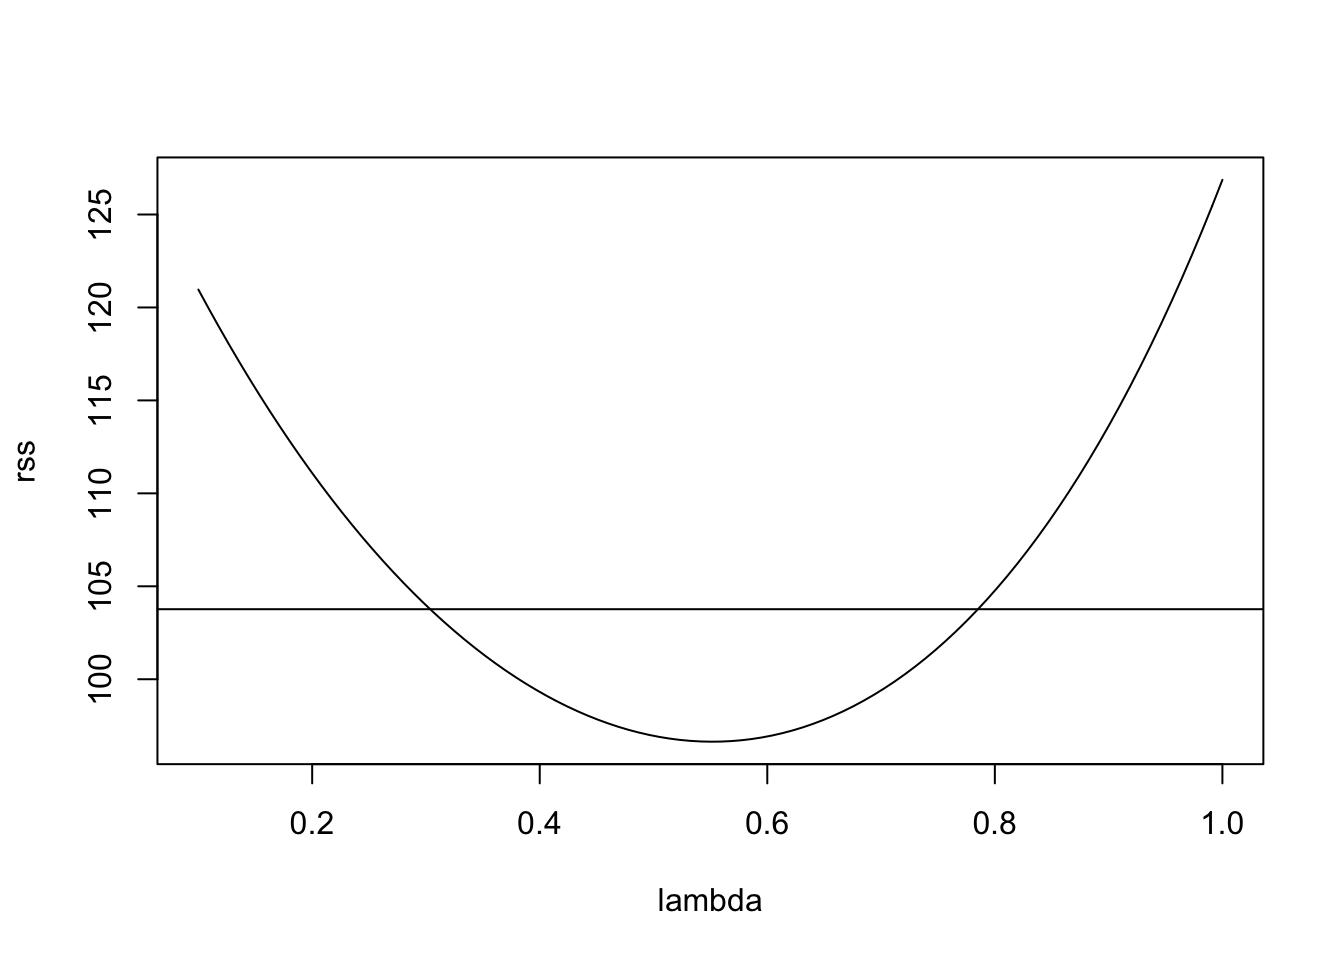
\includegraphics{MATH3714_files/figure-latex/electric5-1.pdf}

This suggests the range of reasonable \(\lambda\) values to be

\begin{Shaded}
\begin{Highlighting}[]
\FunctionTok{range}\NormalTok{(lambda[}\FunctionTok{which}\NormalTok{(rss }\SpecialCharTok{\textless{}=}\NormalTok{ cutoff)])}
\end{Highlighting}
\end{Shaded}

\begin{Shaded}
\begin{Highlighting}[]
\NormalTok{\# [1] 0.307 0.784}
\end{Highlighting}
\end{Shaded}

The value \(\lambda = 1\) (no transformation) is not contained in the interval,
suggesting that a transformation may be helpful.
Choosing a ``simple'' value inside the interval and close to the minimum,
we try \(\lambda = 0.5\). This leads to the following transformation:
\begin{equation*}
  y'
  = 2\sqrt{g} (\sqrt{y}-1).
\end{equation*}
Up to the shift and scaling, this just takes the square root of the data.

\begin{Shaded}
\begin{Highlighting}[]
\NormalTok{y.prime }\OtherTok{\textless{}{-}} \FunctionTok{sqrt}\NormalTok{(y)}
\FunctionTok{plot}\NormalTok{(x, y.prime,}
     \AttributeTok{xlab=}\StringTok{"energy usage [kWh]"}\NormalTok{, }\AttributeTok{ylab=}\StringTok{"sqrt{-}transformed y"}\NormalTok{)}
\NormalTok{m3 }\OtherTok{\textless{}{-}} \FunctionTok{lm}\NormalTok{(y.prime }\SpecialCharTok{\textasciitilde{}}\NormalTok{ x)}
\FunctionTok{abline}\NormalTok{(m3)}
\end{Highlighting}
\end{Shaded}

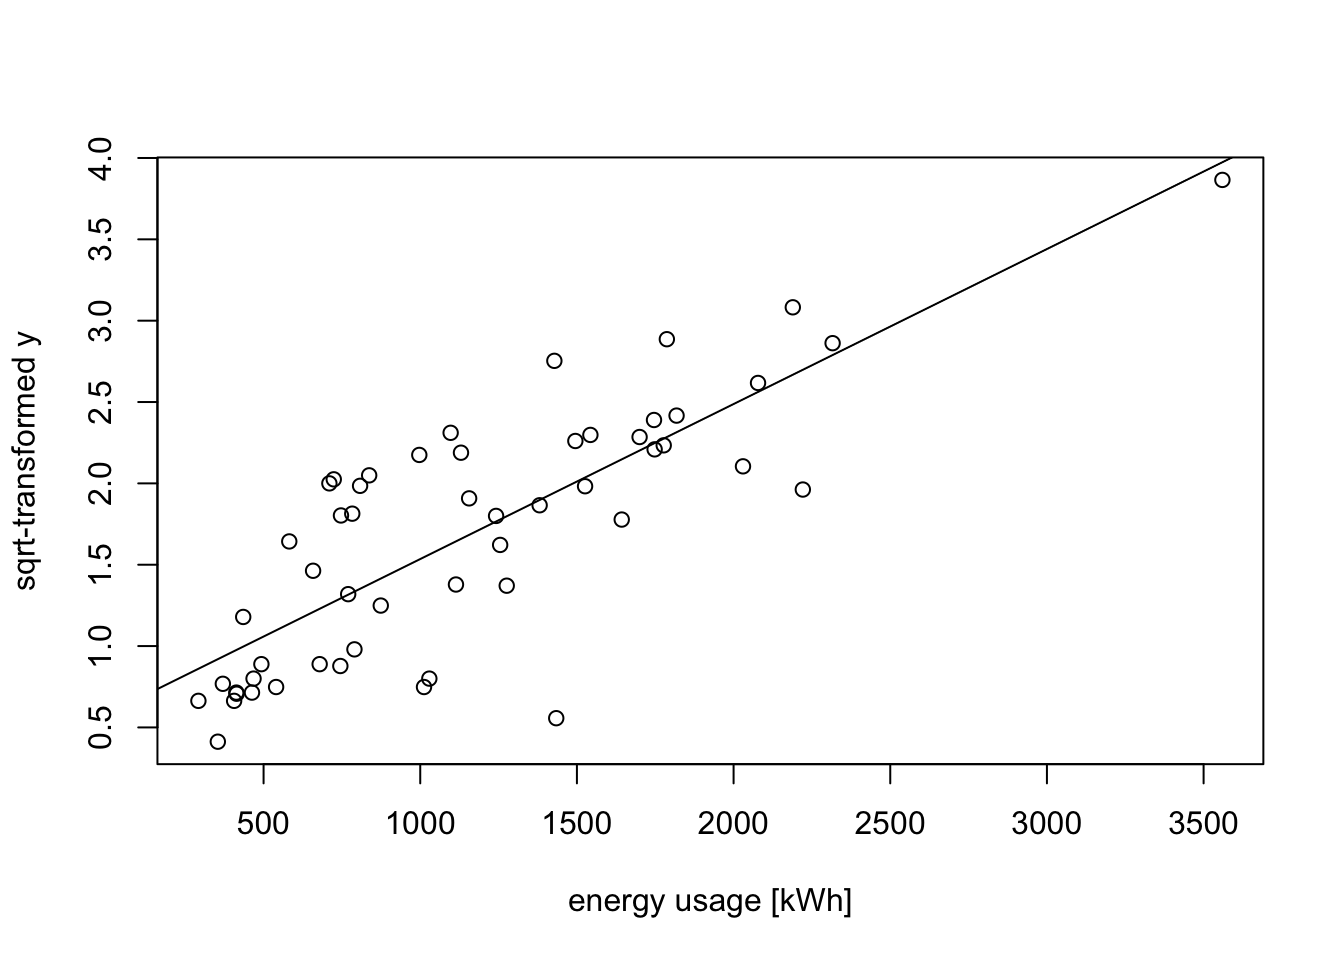
\includegraphics{MATH3714_files/figure-latex/electric6-1.pdf}

To see whether the variance of the residuals has improved, we consider
a residual plot:

\begin{Shaded}
\begin{Highlighting}[]
\FunctionTok{plot}\NormalTok{(}\FunctionTok{fitted}\NormalTok{(m3), }\FunctionTok{resid}\NormalTok{(m3),}
     \AttributeTok{xlab =} \StringTok{"fitted values"}\NormalTok{, }\AttributeTok{ylab =} \StringTok{"residuals for sqrt{-}transform"}\NormalTok{)}
\FunctionTok{abline}\NormalTok{(}\AttributeTok{h =} \DecValTok{0}\NormalTok{)}
\end{Highlighting}
\end{Shaded}

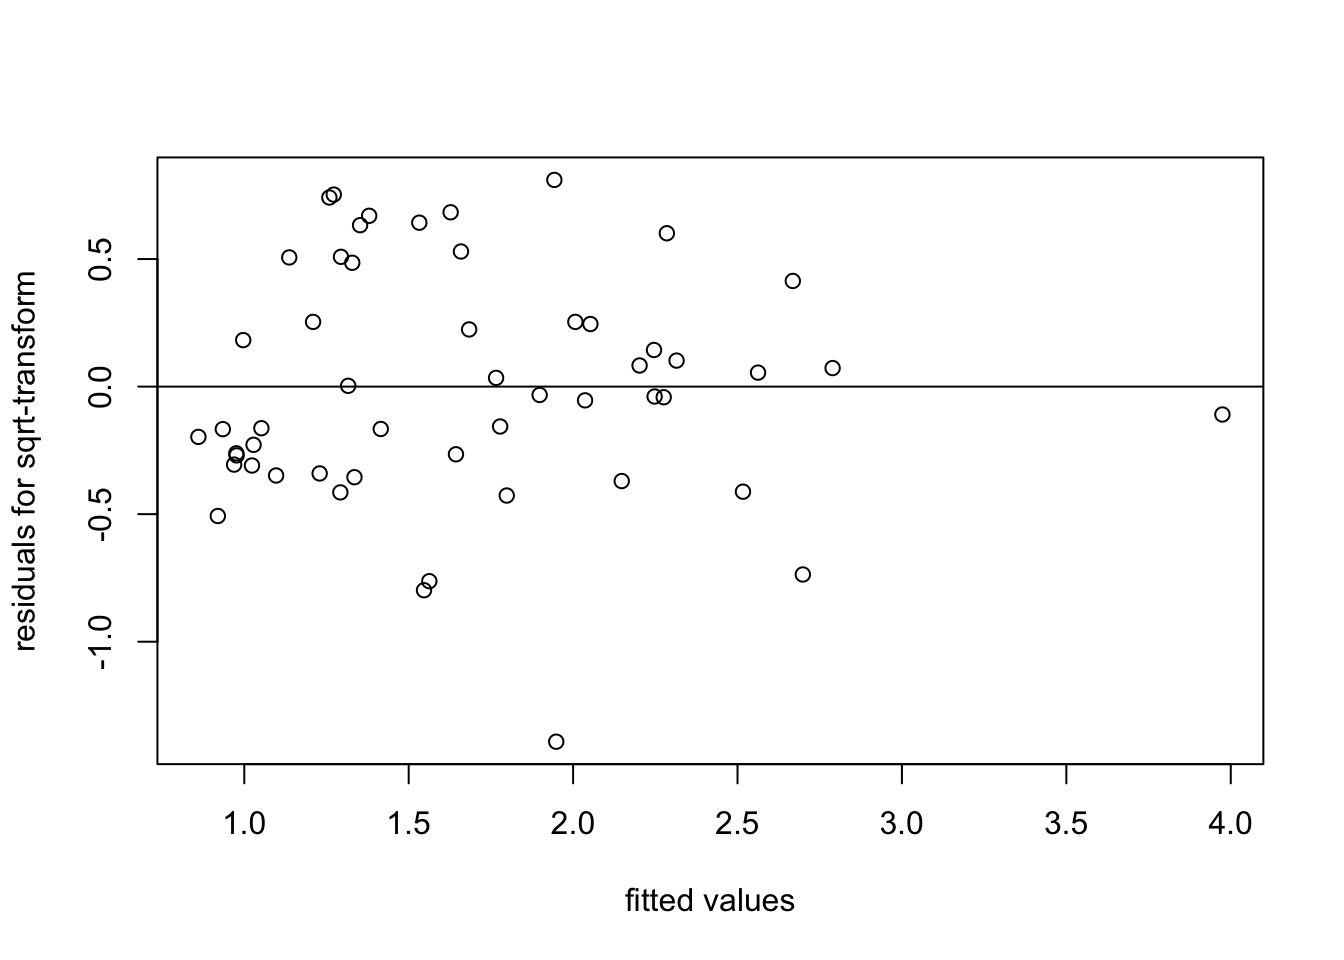
\includegraphics{MATH3714_files/figure-latex/electric7-1.pdf}

We see that the spread of the residuals has indeed improved, when compared to
fitting the original data.
\end{example}

\hypertarget{orthogonal-inputs}{%
\subsection{Orthogonal Inputs}\label{orthogonal-inputs}}

So far, this chapter has been concerned with what to do when there are problems
with a given model. In some cases we have the chance to ``plan ahead'' so that
problems are less likely to occur.

Collinearity occurs when there is high correlation amongst the explanatory
variables. In some situations we have the opportunity to \emph{choose} the design
space \(X\). In these cases, there are advantages in creating design variables
which are orthogonal, thus avoiding or reducing problems caused by
collinearity.

\begin{example}
Suppose we have observations \((x_i, y_i)\) for
\(i\in \{1, \ldots, n\}\) and we want to fit a polynomial model of the form
\begin{equation*}
  Y_i
  = \beta_0 + \beta_1 x_i + \beta_2 x_i^2 + \cdots + \beta_p x_i^p + \varepsilon_i.
\end{equation*}

If we use the actual \(x_i\) to create new variables, say \(x_j = x^j\), then
severe multicollinearity can arise. For example, for
\begin{equation*}
  x
  = (10000, 10001, \ldots, 10010),
\end{equation*}
we have
\begin{equation*}
  x^2
  = 10^8 + (0, 20001, 40004, \ldots, 200100)
\end{equation*}
and \(\mathop{\mathrm{cor}}(x, x^2) \approx 1 - 9.74\times 10^{-9}\):

\begin{Shaded}
\begin{Highlighting}[]
\NormalTok{x }\OtherTok{\textless{}{-}} \FunctionTok{seq}\NormalTok{(}\DecValTok{10000}\NormalTok{, }\DecValTok{10010}\NormalTok{)}
\FunctionTok{cor}\NormalTok{(x, x}\SpecialCharTok{\^{}}\DecValTok{2}\NormalTok{)}
\end{Highlighting}
\end{Shaded}

\begin{Shaded}
\begin{Highlighting}[]
\NormalTok{\# [1] 1}
\end{Highlighting}
\end{Shaded}

\begin{Shaded}
\begin{Highlighting}[]
\DecValTok{1} \SpecialCharTok{{-}} \FunctionTok{cor}\NormalTok{(x, x}\SpecialCharTok{\^{}}\DecValTok{2}\NormalTok{)}
\end{Highlighting}
\end{Shaded}

\begin{Shaded}
\begin{Highlighting}[]
\NormalTok{\# [1] 9.740257e{-}09}
\end{Highlighting}
\end{Shaded}

\begin{Shaded}
\begin{Highlighting}[]
\NormalTok{X }\OtherTok{\textless{}{-}} \FunctionTok{cbind}\NormalTok{(}\DecValTok{1}\NormalTok{, x, x}\SpecialCharTok{\^{}}\DecValTok{2}\NormalTok{)}
\FunctionTok{kappa}\NormalTok{(}\FunctionTok{t}\NormalTok{(X) }\SpecialCharTok{\%*\%}\NormalTok{ X, }\AttributeTok{exact =} \ConstantTok{TRUE}\NormalTok{)}
\end{Highlighting}
\end{Shaded}

\begin{Shaded}
\begin{Highlighting}[]
\NormalTok{\# [1] 1.47006e+23}
\end{Highlighting}
\end{Shaded}

The first result, for the correlation, is shown as \(1\) due to rounding.
The internal number representation of the correlation is actually less than
\(1\) and we can print the difference \texttt{1\ -\ cor(x,\ x\^{}2)} to get the result
stated above. Since this difference is close to \(0\) (instead of close to \(1\)),
R can now use scientific notation to show the very small result. The final line
of the output shows that the condition number is greater than \(10^{23}\),
so the problem indeed suffers severe multicollinearity.

We can greatly improve the conditioning of the problem
by using the centred data \(x^\ast_i = x_i - \bar x\) before taking powers:

\begin{Shaded}
\begin{Highlighting}[]
\NormalTok{x.star }\OtherTok{\textless{}{-}}\NormalTok{ x }\SpecialCharTok{{-}} \FunctionTok{mean}\NormalTok{(x)}
\FunctionTok{cor}\NormalTok{(x.star, x.star}\SpecialCharTok{\^{}}\DecValTok{2}\NormalTok{)}
\end{Highlighting}
\end{Shaded}

\begin{Shaded}
\begin{Highlighting}[]
\NormalTok{\# [1] 0}
\end{Highlighting}
\end{Shaded}

\begin{Shaded}
\begin{Highlighting}[]
\NormalTok{X.star }\OtherTok{\textless{}{-}} \FunctionTok{cbind}\NormalTok{(}\DecValTok{1}\NormalTok{, x.star, x.star}\SpecialCharTok{\^{}}\DecValTok{2}\NormalTok{)}
\FunctionTok{kappa}\NormalTok{(}\FunctionTok{t}\NormalTok{(X.star) }\SpecialCharTok{\%*\%}\NormalTok{ X.star, }\AttributeTok{exact =} \ConstantTok{TRUE}\NormalTok{)}
\end{Highlighting}
\end{Shaded}

\begin{Shaded}
\begin{Highlighting}[]
\NormalTok{\# [1] 408.7796}
\end{Highlighting}
\end{Shaded}

Now the correlation between \(x^\ast\) and \((x^\ast)^2\) is exactly zero,
and the condition number is much improved.
\end{example}

A more systematic approach to choose input variables for polynomial regression
is to use \textbf{orthogonal polynomials} of the form
\begin{align*}
  \psi_0(x) &=  1 \\
  \psi_1(x) &=  \alpha_{1,1} x + \alpha_{1,0} \\
  \psi_2(x) &=  \alpha_{2,2} x^2 + \alpha_{2,1} x + \alpha_{2,0} \\
  &\vdots \\
\end{align*}
where the coefficients \(\alpha_{j,k}\) are chosen such that
\begin{equation*}
  \sum_{i=1}^n \psi_j(x_i) \psi_k(x_i)
  = 0
\end{equation*}
for all \(j, k \in \{0, \ldots, p\}\) with \(j \neq k\). We can then use
input variables
\begin{equation*}
  x_j = \psi_j(x)
\end{equation*}
for \(j \in \{0, \ldots, p\}\) to get a design matrix \(X\) such that
\begin{align*}
  (X^\top X)_{jk}
  &= \sum_{i=1}^n X_{ij} X_{ik} \\
  &= \sum_{i=1}^n \psi_j(x_i) \psi_k(x_i) \\
  &= 0
\end{align*}
for all \(j, k \in \{0, \ldots, p\}\) with \(j \neq k\). In this case the columns
of \(X\) are orthogonal and there is no multicollinearity.
Our model is now
\begin{align*}
  y_i
  &= \beta_0 + \beta_1 x_{i,1} + \cdots + \beta_p x_{i,p} + \varepsilon_i \\
  &= \beta_0 \psi_0(x_i) + \beta_1 \psi_1(x_i) + \beta_2 \psi_2(x_i) + \cdots + \beta_p \psi_p(x_i) + \varepsilon_i.
\end{align*}
Since \(X^\top X\) is diagonal, the inverse of this matrix is trivial to
compute. If we denote the diagonal elements by
\begin{equation*}
  A_j
  = (X^\top X)_{jj},
\end{equation*}
then \(X^\top X = \mathrm{diag}(A_0, \ldots, A_p)\) and
\((X^\top X)^{-1} = \mathrm{diag}(1/A_0, \ldots, 1/A_p)\). Thus we get
\begin{align*}
  \hat\beta_j
  &= \bigl( (X^\top X)^{-1} X^\top y \bigr)_j \\
  &= \frac{1}{A_j} \sum_{i=1}^n \psi_j(x_i) y_i
\end{align*}
and similarly, using equation~\eqref{eq:beta-hat-i}, we find
\begin{equation*}
  \mathop{\mathrm{Var}}( \hat\beta_j )
  = \frac{\sigma^2}{A_j}.
\end{equation*}

An additional advantage of this approach is, that we can add another term,
\(\psi_{p+1}(x)\), without changing the previous estimates of the regression
coefficients. Since \(X^\top X\) is diagonal, the change will not affect the
estimates \(\hat\beta_j\) for \(j\in \{0, \ldots, p\}\) (but the change will affect
\(\sigma^2\)).

\begin{example}
In R we can create specific orthogonal entries for polynomial regression using
the command \texttt{poly(x,\ p)}. The output of this function is a matrix
with elements \(\psi_j(x_i)\) for \(j \in \{1, \ldots, p\}\) (omitting the intercept)
and \(i \in \{1, \ldots, n\}\). Continuing from the example above we find

\begin{Shaded}
\begin{Highlighting}[]
\NormalTok{x }\OtherTok{\textless{}{-}} \FunctionTok{seq}\NormalTok{(}\DecValTok{10000}\NormalTok{, }\DecValTok{10010}\NormalTok{)}
\NormalTok{X }\OtherTok{\textless{}{-}} \FunctionTok{cbind}\NormalTok{(}\DecValTok{1}\NormalTok{, }\FunctionTok{poly}\NormalTok{(x, }\DecValTok{2}\NormalTok{)) }\CommentTok{\# manually prepend a column of ones}
\FunctionTok{round}\NormalTok{(}\FunctionTok{t}\NormalTok{(X) }\SpecialCharTok{\%*\%}\NormalTok{ X, }\DecValTok{5}\NormalTok{)}
\end{Highlighting}
\end{Shaded}

\begin{Shaded}
\begin{Highlighting}[]
\NormalTok{\#      1 2}
\NormalTok{\#   11 0 0}
\NormalTok{\# 1  0 1 0}
\NormalTok{\# 2  0 0 1}
\end{Highlighting}
\end{Shaded}

Different from our previous approach, the last two columns are now also
orthogonal to the columns of ones. This further improves the conditioning
of the design matrix:

\begin{Shaded}
\begin{Highlighting}[]
\FunctionTok{kappa}\NormalTok{(X, }\AttributeTok{exact =} \ConstantTok{TRUE}\NormalTok{)}
\end{Highlighting}
\end{Shaded}

\begin{Shaded}
\begin{Highlighting}[]
\NormalTok{\# [1] 3.316625}
\end{Highlighting}
\end{Shaded}

We see that the use of orthogonal polynomials entirely eliminated any
problems with multicollinearity.
\end{example}

\begin{example}

To illustrate the use of \texttt{poly()} for fitting a polynomial model to
real data, we use the built-in \texttt{cars} dataset in R. This dataset
contains historic data (from the 1920s) about the speed of cars (in mph) and
the distances taken to stop (in ft). We first fit a second order polynomial
to the data using the naive approach:

\begin{Shaded}
\begin{Highlighting}[]
\NormalTok{m1 }\OtherTok{\textless{}{-}} \FunctionTok{lm}\NormalTok{(dist }\SpecialCharTok{\textasciitilde{}}\NormalTok{ speed }\SpecialCharTok{+} \FunctionTok{I}\NormalTok{(speed}\SpecialCharTok{\^{}}\DecValTok{2}\NormalTok{), }\AttributeTok{data =}\NormalTok{ cars)}
\FunctionTok{plot}\NormalTok{(cars)}
\FunctionTok{lines}\NormalTok{(}\FunctionTok{predict}\NormalTok{(m1, }\AttributeTok{newdata =} \FunctionTok{data.frame}\NormalTok{(}\AttributeTok{speed=}\FunctionTok{seq}\NormalTok{(}\DecValTok{0}\NormalTok{, }\DecValTok{30}\NormalTok{, }\AttributeTok{l=}\DecValTok{31}\NormalTok{))),}
      \AttributeTok{col=}\StringTok{"blue"}\NormalTok{)}
\end{Highlighting}
\end{Shaded}

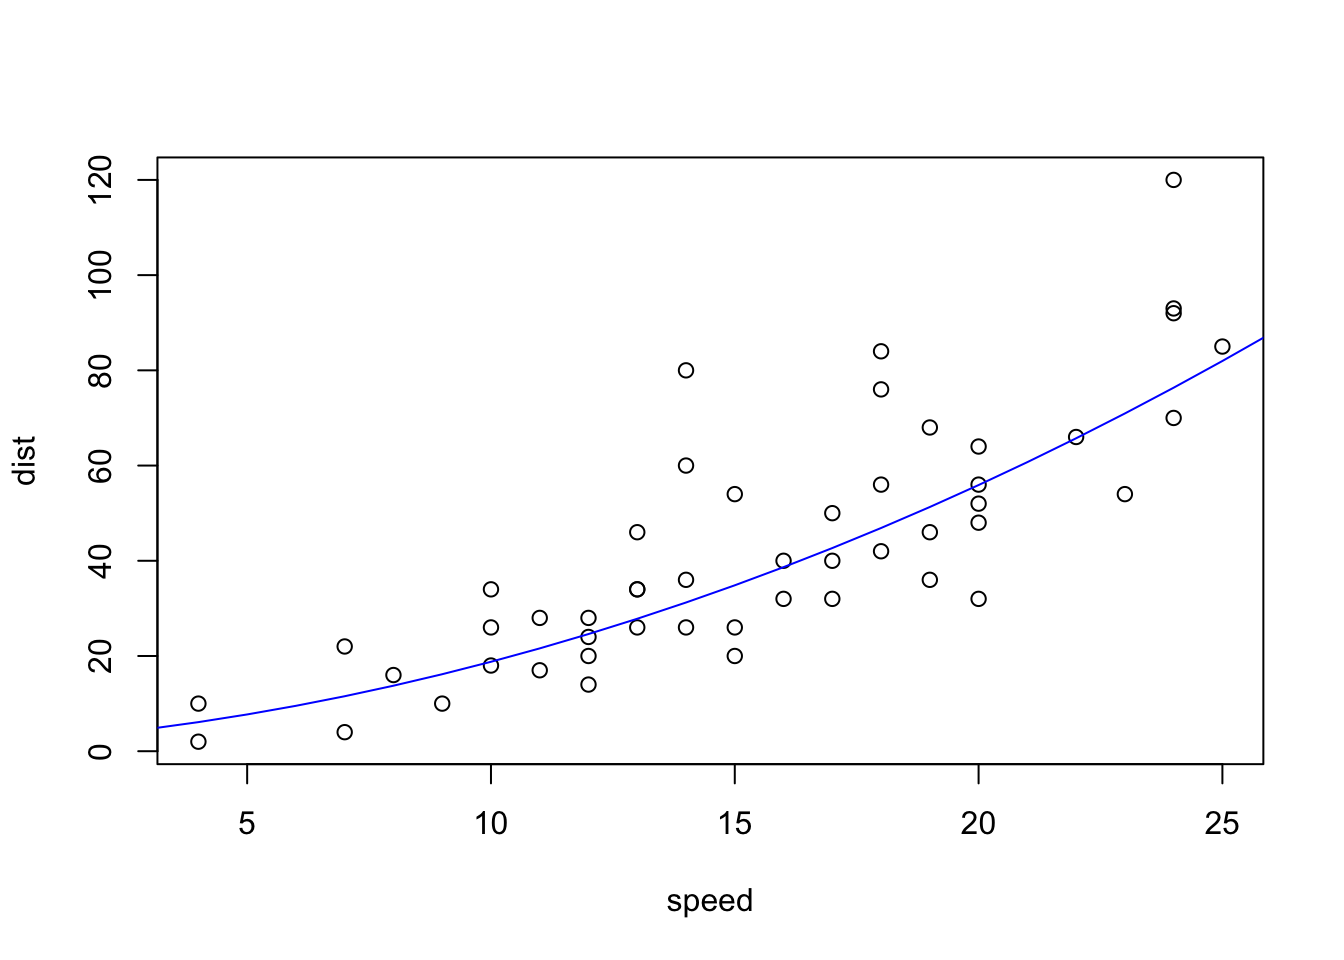
\includegraphics{MATH3714_files/figure-latex/cars-1.pdf}

Checking the condition number, we see that there is severe multicollinearity:

\begin{Shaded}
\begin{Highlighting}[]
\FunctionTok{kappa}\NormalTok{(m1, }\AttributeTok{exact =} \ConstantTok{TRUE}\NormalTok{)}
\end{Highlighting}
\end{Shaded}

\begin{Shaded}
\begin{Highlighting}[]
\NormalTok{\# [1] 2160.976}
\end{Highlighting}
\end{Shaded}

We can also see that none of the coefficients is significantly different from
zero, while the F-test rejects the hypothesis that the vector of all regression
coefficients is zero. We have seen previously that this effect can be an
indication of multicollinearity.

\begin{Shaded}
\begin{Highlighting}[]
\FunctionTok{summary}\NormalTok{(m1)}
\end{Highlighting}
\end{Shaded}

\begin{Shaded}
\begin{Highlighting}[]
\NormalTok{\# }
\NormalTok{\# Call:}
\NormalTok{\# lm(formula = dist \textasciitilde{} speed + I(speed\^{}2), data = cars)}
\NormalTok{\# }
\NormalTok{\# Residuals:}
\NormalTok{\#     Min      1Q  Median      3Q     Max }
\NormalTok{\# {-}28.720  {-}9.184  {-}3.188   4.628  45.152 }
\NormalTok{\# }
\NormalTok{\# Coefficients:}
\NormalTok{\#             Estimate Std. Error t value Pr(\textgreater{}|t|)}
\NormalTok{\# (Intercept)  2.47014   14.81716   0.167    0.868}
\NormalTok{\# speed        0.91329    2.03422   0.449    0.656}
\NormalTok{\# I(speed\^{}2)   0.09996    0.06597   1.515    0.136}
\NormalTok{\# }
\NormalTok{\# Residual standard error: 15.18 on 47 degrees of freedom}
\NormalTok{\# Multiple R{-}squared:  0.6673,  Adjusted R{-}squared:  0.6532 }
\NormalTok{\# F{-}statistic: 47.14 on 2 and 47 DF,  p{-}value: 5.852e{-}12}
\end{Highlighting}
\end{Shaded}

We can fit an improved model using orthogonal polynomials. Since \texttt{lm()}
automatically adds the intercept, we don't need to prepend a column of ones to
the \texttt{poly()} output here.

\begin{Shaded}
\begin{Highlighting}[]
\NormalTok{m2 }\OtherTok{\textless{}{-}} \FunctionTok{lm}\NormalTok{(dist }\SpecialCharTok{\textasciitilde{}} \FunctionTok{poly}\NormalTok{(speed, }\DecValTok{2}\NormalTok{), }\AttributeTok{data =}\NormalTok{ cars)}
\FunctionTok{kappa}\NormalTok{(m2)}
\end{Highlighting}
\end{Shaded}

\begin{Shaded}
\begin{Highlighting}[]
\NormalTok{\# [1] 6.670129}
\end{Highlighting}
\end{Shaded}

We see that in the new model there are no problems with multicollinearity any
more. The new model also has coefficients which are significantly different
from zero:

\begin{Shaded}
\begin{Highlighting}[]
\FunctionTok{summary}\NormalTok{(m2)}
\end{Highlighting}
\end{Shaded}

\begin{Shaded}
\begin{Highlighting}[]
\NormalTok{\# }
\NormalTok{\# Call:}
\NormalTok{\# lm(formula = dist \textasciitilde{} poly(speed, 2), data = cars)}
\NormalTok{\# }
\NormalTok{\# Residuals:}
\NormalTok{\#     Min      1Q  Median      3Q     Max }
\NormalTok{\# {-}28.720  {-}9.184  {-}3.188   4.628  45.152 }
\NormalTok{\# }
\NormalTok{\# Coefficients:}
\NormalTok{\#                 Estimate Std. Error t value Pr(\textgreater{}|t|)    }
\NormalTok{\# (Intercept)       42.980      2.146  20.026  \textless{} 2e{-}16 ***}
\NormalTok{\# poly(speed, 2)1  145.552     15.176   9.591 1.21e{-}12 ***}
\NormalTok{\# poly(speed, 2)2   22.996     15.176   1.515    0.136    }
\NormalTok{\# {-}{-}{-}}
\NormalTok{\# Signif. codes:  0 \textquotesingle{}***\textquotesingle{} 0.001 \textquotesingle{}**\textquotesingle{} 0.01 \textquotesingle{}*\textquotesingle{} 0.05 \textquotesingle{}.\textquotesingle{} 0.1 \textquotesingle{} \textquotesingle{} 1}
\NormalTok{\# }
\NormalTok{\# Residual standard error: 15.18 on 47 degrees of freedom}
\NormalTok{\# Multiple R{-}squared:  0.6673,  Adjusted R{-}squared:  0.6532 }
\NormalTok{\# F{-}statistic: 47.14 on 2 and 47 DF,  p{-}value: 5.852e{-}12}
\end{Highlighting}
\end{Shaded}

\end{example}

\textbf{Summary}

\begin{itemize}
\tightlist
\item
  We have seen different transformations which can be used
  to transform a nonlinear model into a linear one.
\item
  We have discussed transformations which can stabilise the
  variance of the errors in the model.
\item
  We have seen how orthogonal polynomials can be used to avoid
  multicollinearity in polynomial regression.
\end{itemize}

\clearpage

\hypertarget{S12-ridge}{%
\section{Ridge Regression}\label{S12-ridge}}

In cases where \(X\) shows approximate multicollinearity, the parameter estimates
\(\hat\beta\) have coefficients with large variance. In case of exact
multicollinearity, \(\hat\beta\) is no longer uniquely defined, and the minimum
of the residual sum of squares is attained on an (unbounded) subspace of the
parameter space. In both cases, a more stable estimate can be obtained by
changing the estimation procedure to include an additional penalty term which
discourages ``large'' values of \(\hat\beta\). This is the idea of ridge
regression. In this section we will see that the resulting estimates are
biased, but sometimes have smaller mean squared error than the least squares
estimator.

\hypertarget{definition-the-estimator}{%
\subsection{Definition the Estimator}\label{definition-the-estimator}}

\begin{definition}
In multiple linear regression, the \textbf{ridge regression} estimate for
the parameter vector \(\beta\) is given by
\begin{equation}
  \hat\beta^{(\lambda)}
  = \mathop{\mathrm{arg\,min}}\limits_\beta \Bigl(
      \sum_{i=1}^n \bigl( y_i - x_i^\top \beta \bigr)^2
      + \lambda \|\beta\|^2
    \Bigr).
\end{equation}
The parameter \(\lambda \geq 0\) is called the \textbf{regularisation parameter}.
\end{definition}

Here we write \(\mathop{\mathrm{arg\,min}}\limits\nolimits_\beta (\cdots)\) to denote the value of \(\beta\)
which minimises the expression on the right-hand side, and \(\|\beta\|\)
denotes the Euclidean norm of the vector \(\beta\), \emph{i.e.}
\begin{equation*}
  \|\beta\|^2
  = \sum_{j=0}^p \beta_j^2.
\end{equation*}

The term being minimised is
\begin{equation*}
  r^{(\lambda)}
  = \sum_{i=1}^n \bigl( y_i - x_i^\top \beta \bigr)^2
      + \lambda \|\beta\|^2,
\end{equation*}
consisting of the residual sum of squares plus a penalty term. The
regularisation parameter \(\lambda\) controls the relative weight of these two
terms. For large \(\lambda\), the main objective to minimise the norm
\(\|\beta\|\) and one can show that \(\lim_{\lambda \to\infty} \hat\beta^{(\lambda)} = 0\). For \(\lambda \downarrow 0\) only the residual sum
of squares is left and if \(X^\top X\) is invertible we get \(\hat\beta^{(0)} = \hat\beta\), \emph{i.e.}~here the ridge regression estimate coincides with the least
squares estimate.

As in lemma~\ref{lem:multiple-LSQ} we can find an explicit formula
for the ridge regression estimate. For this we write \(r^{(\lambda)}\)
as
\begin{equation*}
  r^{(\lambda)}
  = (y - X\top \beta)^\top (y - X\top \beta )
      + \lambda \beta^\top \beta
\end{equation*}
and then take derivatives to find the minimum. The result is
given by
\begin{equation}
  \hat\beta^{(\lambda)}
  = (X^\top X + \lambda I)^{-1} X^\top y.    \label{eq:1523}
\end{equation}

\begin{example}
\protect\hypertarget{exm:knorkel}{}\label{exm:knorkel}To illustrate the method, we compute the ridge regression estimate for
a badly conditioned toy dataset.

\begin{Shaded}
\begin{Highlighting}[]
\CommentTok{\# fix the true parameters for our simulated data:}
\NormalTok{beta }\OtherTok{\textless{}{-}} \FunctionTok{c}\NormalTok{(}\DecValTok{0}\NormalTok{, .}\DecValTok{5}\NormalTok{, .}\DecValTok{5}\NormalTok{)}
\NormalTok{sigma }\OtherTok{\textless{}{-}} \FloatTok{0.01}

\FunctionTok{set.seed}\NormalTok{(}\DecValTok{20211112}\NormalTok{)}
\NormalTok{x1 }\OtherTok{\textless{}{-}} \FunctionTok{c}\NormalTok{(}\FloatTok{1.01}\NormalTok{, }\FloatTok{2.00}\NormalTok{, }\FloatTok{2.99}\NormalTok{, }\FloatTok{4.02}\NormalTok{, }\FloatTok{5.01}\NormalTok{, }\FloatTok{5.99}\NormalTok{)}
\NormalTok{x2 }\OtherTok{\textless{}{-}} \FunctionTok{c}\NormalTok{(}\FloatTok{0.98}\NormalTok{, }\FloatTok{1.99}\NormalTok{, }\FloatTok{3.00}\NormalTok{, }\FloatTok{4.00}\NormalTok{, }\FloatTok{4.99}\NormalTok{, }\FloatTok{6.00}\NormalTok{)}
\CommentTok{\# beta[1] in R corresponds to \textbackslash{}beta\_0, beta[2] = \textbackslash{}beta\_1, beta[3] = \textbackslash{}beta\_2}
\NormalTok{y }\OtherTok{\textless{}{-}}\NormalTok{ beta[}\DecValTok{1}\NormalTok{] }\SpecialCharTok{+}\NormalTok{ beta[}\DecValTok{2}\NormalTok{] }\SpecialCharTok{*}\NormalTok{ x1 }\SpecialCharTok{+}\NormalTok{ beta[}\DecValTok{3}\NormalTok{] }\SpecialCharTok{*}\NormalTok{ x2 }\SpecialCharTok{+} \FunctionTok{rnorm}\NormalTok{(}\DecValTok{6}\NormalTok{, }\DecValTok{0}\NormalTok{, sigma)}

\NormalTok{lambda }\OtherTok{\textless{}{-}} \FloatTok{0.01}
\NormalTok{X }\OtherTok{\textless{}{-}} \FunctionTok{model.matrix}\NormalTok{(y }\SpecialCharTok{\textasciitilde{}}\NormalTok{ x1 }\SpecialCharTok{+}\NormalTok{ x2)}
\NormalTok{beta.ridge }\OtherTok{\textless{}{-}} \FunctionTok{solve}\NormalTok{(}\FunctionTok{t}\NormalTok{(X) }\SpecialCharTok{\%*\%}\NormalTok{ X }\SpecialCharTok{+}\NormalTok{ lambda }\SpecialCharTok{*} \FunctionTok{diag}\NormalTok{(}\FunctionTok{ncol}\NormalTok{(X)), }\FunctionTok{t}\NormalTok{(X) }\SpecialCharTok{\%*\%}\NormalTok{ y)}
\NormalTok{beta.ridge[,}\DecValTok{1}\NormalTok{] }\CommentTok{\# get first column instead of n × 1 matrix, for tidiness}
\end{Highlighting}
\end{Shaded}

\begin{Shaded}
\begin{Highlighting}[]
\NormalTok{\# (Intercept)          x1          x2 }
\NormalTok{\# {-}0.01620501  0.52739367  0.47343531}
\end{Highlighting}
\end{Shaded}

For comparison, we also compute the least squares estimate:

\begin{Shaded}
\begin{Highlighting}[]
\NormalTok{m }\OtherTok{\textless{}{-}} \FunctionTok{lm}\NormalTok{(y }\SpecialCharTok{\textasciitilde{}}\NormalTok{ x1 }\SpecialCharTok{+}\NormalTok{ x2)}
\FunctionTok{coef}\NormalTok{(m)}
\end{Highlighting}
\end{Shaded}

\begin{Shaded}
\begin{Highlighting}[]
\NormalTok{\# (Intercept)          x1          x2 }
\NormalTok{\# {-}0.02935851  1.03064453 {-}0.02749857}
\end{Highlighting}
\end{Shaded}

We see that despite the small value of \(\lambda\) there is a considerable
difference between the estimated values \(\hat\beta\) and
\(\hat\beta^{(\lambda)}\) in this example. Experimenting with different
values of the seed also shows that the variance of \(\hat\beta^{(\lambda)}\)
is much smaller than the variance of \(\hat\beta\). In the next section
we will see a theoretical explanation for this fact.
\end{example}

For \(\lambda > 0\) and \(v \neq 0\) we have \(\|v\| > 0\) and thus
\begin{align*}
  \| (X^\top X + \lambda I) v \|^2
  &= v^\top (X^\top X + \lambda I)^\top (X^\top X + \lambda I) v \\
  &= v^\top X^\top X X^\top X v + 2 \lambda v^\top X^\top X v + \lambda^2 v^\top v \\
  &= \| X X^\top X v \|^2 + 2 \lambda \| X v \|^2 + \lambda^2 \| v \|^2 \\
  &\geq \lambda^2 \| v \|^2 \\
  &> 0.
\end{align*}
This shows, by theorem~\ref{thm:matrix-inverse}, that
the matrix \(X^\top X + \lambda I\)
is invertible for every \(\lambda > 0\). Thus the
ridge regression estimate for \(\lambda > 0\) is always uniquely defined,
even in cases where the least squares estimate is \emph{not} uniquely defined.

There are variants of the method where the penalty term \(\|\beta\|^2\) is is
replaced with a different penalty term. One example of this is Lasso (least
absolute shrinkage and selection operator) regression, which uses \(\|\beta\|_1 = \sum_{j=0}^p |\beta_j|\) as the penalty term.

Outside statistics, ridge regression is known as \textbf{Tikhonov regularisation}.

\hypertarget{properties-of-the-estimate}{%
\subsection{Properties of the Estimate}\label{properties-of-the-estimate}}

Using the statistical model
\begin{equation*}
  Y = X \beta + \varepsilon
\end{equation*}
as before, we have
\begin{align*}
  \hat\beta^{(\lambda)}
  &= (X^\top X + \lambda I)^{-1} X^\top Y \\
  &= (X^\top X + \lambda I)^{-1} X^\top (X \beta + \varepsilon) \\
  &= (X^\top X + \lambda I)^{-1} (X^\top X + \lambda I) \beta \\
    &\hskip15mm - (X^\top X + \lambda I)^{-1} \lambda I \beta \\
    &\hskip15mm + (X^\top X + \lambda I)^{-1} X^\top \varepsilon
\end{align*}
and simplifying the first term on the right-hand side we get
\begin{equation}
  \hat\beta^{(\lambda)}
  = \beta
    - \lambda (X^\top X + \lambda I)^{-1} \beta
    + (X^\top X + \lambda I)^{-1} X^\top \varepsilon.   \label{eq:ridge-def}
\end{equation}

\hypertarget{bias}{%
\subsubsection{Bias}\label{bias}}

Using the formula for \(\hat\beta^{(\lambda)}\) we get
\begin{equation*}
  \mathbb{E}\bigl( \hat\beta^{(\lambda)} \bigr)
  = \beta - \lambda (X^\top X + \lambda I)^{-1} \beta + 0
\end{equation*}
and thus
\begin{equation*}
  \mathop{\mathrm{bias}}\bigl( \hat\beta^{(\lambda)} \bigr)
  = - \lambda (X^\top X + \lambda I)^{-1} \beta.
\end{equation*}
Since this term in general is non-zero, we see that \(\hat\beta^{(\lambda)}\)
is a biased estimate. The amount of bias depends on the unknown, true
coefficient vector~\(\beta\).

\hypertarget{variance}{%
\subsubsection{Variance}\label{variance}}

The covariance matrix of the vector \(\hat\beta^{(\lambda)}\) is given
by
\begin{align*}
  \mathop{\mathrm{Cov}}\bigl(\hat\beta^{(\lambda)}\bigr)
  &= \mathop{\mathrm{Cov}}\Bigl(
      \beta
      - \lambda (X^\top X + \lambda I)^{-1} X^\top X \beta
      + (X^\top X + \lambda I)^{-1} X^\top \varepsilon
    \Bigr) \\
  &= \mathop{\mathrm{Cov}}\Bigl(
      (X^\top X + \lambda I)^{-1} X^\top \varepsilon
    \Bigr) \\
  &= (X^\top X + \lambda I)^{-1} X^\top \mathop{\mathrm{Cov}}(\varepsilon) X (X^\top X + \lambda I)^{-1} \\
  &= \sigma^2 (X^\top X + \lambda I)^{-1} X^\top X (X^\top X + \lambda I)^{-1} \\
  &= \sigma^2 (X^\top X + \lambda I)^{-1} - \lambda \sigma^2 (X^\top X + \lambda I)^{-2}.
\end{align*}
While this is an explicit formula, the resulting covariance matrix
depends on the unknown error variance~\(\sigma^2\).

If \(X^\top X\) is invertible, this covariance will convert to the
covariance of the least squares estimator as \(\lambda \downarrow 0\).
From this we can find the variance of individual components
as \(\mathop{\mathrm{Var}}\bigl( \hat\beta^{(\lambda)}_j \bigr) = \mathop{\mathrm{Cov}}( \hat\beta^{(\lambda)} )_{jj}\).

\hypertarget{mean-squared-error}{%
\subsubsection{Mean Squared Error}\label{mean-squared-error}}

The Mean Squared Error (MSE) of an estimator \(\hat \beta_j\) for \(\beta_j\) is
given by
\begin{equation*}
  \mathop{\mathrm{MSE}}\nolimits( \hat\beta_j )
  = \mathbb{E}\Bigl( \bigl( \hat\beta_j - \beta_j \bigr)^2 \Bigr).
\end{equation*}
It is an easy exercise to show that this can equivalently be written as
\begin{equation*}
  \mathop{\mathrm{MSE}}\nolimits\bigl( \hat\beta_j \bigr)
  = \mathop{\mathrm{Var}}\bigl( \hat\beta_j \bigr) + \mathop{\mathrm{bias}}\bigl( \hat\beta_j \bigr)^2.
\end{equation*}
Using the formulas for the variance and bias from above, we
can find an formula for \(\mathop{\mathrm{MSE}}\nolimits(\hat\beta^{(\lambda)}_j)\),
but the result is hard to interpret. Instead of considering these analytical
expressions, we illustrate the MSE using a numerical
example.

\begin{example}
Continuing from example~\ref{exm:knorkel} above, we can determine
the MSE for every value of~\(\lambda\). Here we
use the fact that this is simulated data where we know the true
values of \(\beta\) and~\(\sigma^2\).

We start with the bias:

\begin{Shaded}
\begin{Highlighting}[]
\NormalTok{lambda }\OtherTok{\textless{}{-}} \FloatTok{0.1}
\NormalTok{Q }\OtherTok{\textless{}{-}} \FunctionTok{t}\NormalTok{(X) }\SpecialCharTok{\%*\%}\NormalTok{ X }\SpecialCharTok{+}\NormalTok{ lambda }\SpecialCharTok{*} \FunctionTok{diag}\NormalTok{(}\FunctionTok{ncol}\NormalTok{(X))}
\NormalTok{lambda }\SpecialCharTok{*} \FunctionTok{solve}\NormalTok{(Q, }\FunctionTok{t}\NormalTok{(X) }\SpecialCharTok{\%*\%}\NormalTok{ X }\SpecialCharTok{\%*\%}\NormalTok{ beta)}
\end{Highlighting}
\end{Shaded}

\begin{Shaded}
\begin{Highlighting}[]
\NormalTok{\#                     [,1]}
\NormalTok{\# (Intercept) 0.0009178679}
\NormalTok{\# x1          0.0497789499}
\NormalTok{\# x2          0.0499545553}
\end{Highlighting}
\end{Shaded}

For the covariance matrix we get the following:

\begin{Shaded}
\begin{Highlighting}[]
\NormalTok{C1 }\OtherTok{\textless{}{-}} \FunctionTok{solve}\NormalTok{(Q) }\CommentTok{\# Compute the inverse Q\^{}\{{-}1\} ...}
\NormalTok{C2 }\OtherTok{\textless{}{-}}\NormalTok{ C1 }\SpecialCharTok{\%*\%}\NormalTok{ C1 }\CommentTok{\# ... and also Q\^{}\{{-}2\}, to get}
\NormalTok{sigma}\SpecialCharTok{\^{}}\DecValTok{2} \SpecialCharTok{*}\NormalTok{ (C1 }\SpecialCharTok{{-}}\NormalTok{ lambda}\SpecialCharTok{*}\NormalTok{C2) }\CommentTok{\# the covariance matrix.}
\end{Highlighting}
\end{Shaded}

\begin{Shaded}
\begin{Highlighting}[]
\NormalTok{\#               (Intercept)            x1            x2}
\NormalTok{\# (Intercept)  7.291379e{-}05 {-}7.580602e{-}06 {-}9.226941e{-}06}
\NormalTok{\# x1          {-}7.580602e{-}06  3.831264e{-}06 {-}1.540098e{-}06}
\NormalTok{\# x2          {-}9.226941e{-}06 {-}1.540098e{-}06  4.221464e{-}06}
\end{Highlighting}
\end{Shaded}

Now we repeat these calculations in a loop, to plot the MSE
as a function of~\(\lambda\):

\begin{Shaded}
\begin{Highlighting}[]
\NormalTok{lambda }\OtherTok{\textless{}{-}} \DecValTok{10}\SpecialCharTok{\^{}}\FunctionTok{seq}\NormalTok{(}\SpecialCharTok{{-}}\DecValTok{4}\NormalTok{, }\DecValTok{0}\NormalTok{, }\AttributeTok{length.out =} \DecValTok{100}\NormalTok{) }\CommentTok{\# range of lambda to try}
\NormalTok{j.plus}\FloatTok{.1} \OtherTok{\textless{}{-}} \DecValTok{1} \SpecialCharTok{+} \DecValTok{1} \CommentTok{\# we plot the error of \textbackslash{}beta\_1}

\NormalTok{variance }\OtherTok{\textless{}{-}} \FunctionTok{numeric}\NormalTok{(}\FunctionTok{length}\NormalTok{(lambda))}
\NormalTok{bias }\OtherTok{\textless{}{-}} \FunctionTok{numeric}\NormalTok{(}\FunctionTok{length}\NormalTok{(lambda))}
\ControlFlowTok{for}\NormalTok{ (i }\ControlFlowTok{in} \FunctionTok{seq\_along}\NormalTok{(lambda)) \{}
\NormalTok{    lambda.i }\OtherTok{\textless{}{-}}\NormalTok{ lambda[i]}
\NormalTok{    Q }\OtherTok{\textless{}{-}} \FunctionTok{t}\NormalTok{(X) }\SpecialCharTok{\%*\%}\NormalTok{ X }\SpecialCharTok{+}\NormalTok{ lambda.i }\SpecialCharTok{*} \FunctionTok{diag}\NormalTok{(}\FunctionTok{ncol}\NormalTok{(X))}
\NormalTok{    C1 }\OtherTok{\textless{}{-}} \FunctionTok{solve}\NormalTok{(Q)}
\NormalTok{    bias[i] }\OtherTok{\textless{}{-}}\NormalTok{ (lambda.i }\SpecialCharTok{*} \FunctionTok{solve}\NormalTok{(Q, }\FunctionTok{t}\NormalTok{(X) }\SpecialCharTok{\%*\%}\NormalTok{ X }\SpecialCharTok{\%*\%}\NormalTok{ beta))[j.plus}\FloatTok{.1}\NormalTok{]}
\NormalTok{    C2 }\OtherTok{\textless{}{-}}\NormalTok{ C1 }\SpecialCharTok{\%*\%}\NormalTok{ C1}
\NormalTok{    C }\OtherTok{\textless{}{-}}\NormalTok{ C1 }\SpecialCharTok{{-}}\NormalTok{ lambda.i}\SpecialCharTok{*}\NormalTok{C2}
\NormalTok{    variance[i] }\OtherTok{\textless{}{-}}\NormalTok{ sigma}\SpecialCharTok{\^{}}\DecValTok{2} \SpecialCharTok{*}\NormalTok{ C[j.plus}\FloatTok{.1}\NormalTok{, j.plus}\FloatTok{.1}\NormalTok{]}
\NormalTok{\}}
\NormalTok{MSE }\OtherTok{\textless{}{-}}\NormalTok{ variance }\SpecialCharTok{+}\NormalTok{ bias}\SpecialCharTok{\^{}}\DecValTok{2}

\FunctionTok{plot}\NormalTok{(lambda, MSE, }\AttributeTok{type =} \StringTok{"l"}\NormalTok{, }\AttributeTok{log =} \StringTok{"x"}\NormalTok{, }\AttributeTok{ylim =} \FunctionTok{c}\NormalTok{(}\DecValTok{0}\NormalTok{, }\FloatTok{0.1}\NormalTok{))}
\FunctionTok{lines}\NormalTok{(lambda, bias}\SpecialCharTok{\^{}}\DecValTok{2}\NormalTok{, }\AttributeTok{col=}\StringTok{"\#1b9e77"}\NormalTok{, }\AttributeTok{lw =} \DecValTok{3}\NormalTok{)}
\FunctionTok{lines}\NormalTok{(lambda, variance, }\AttributeTok{col=}\StringTok{"\#d95f02"}\NormalTok{, }\AttributeTok{lw =} \DecValTok{3}\NormalTok{)}
\FunctionTok{lines}\NormalTok{(lambda, MSE) }\CommentTok{\# make sure MSE is not obscured by bias/variance}
\FunctionTok{abline}\NormalTok{(}\AttributeTok{v =}\NormalTok{ lambda[}\FunctionTok{which.min}\NormalTok{(MSE)]) }\CommentTok{\# mark the minimum}

\FunctionTok{legend}\NormalTok{(}\StringTok{"topleft"}\NormalTok{,}
       \FunctionTok{c}\NormalTok{(}\StringTok{"bias squared"}\NormalTok{, }\StringTok{"variance"}\NormalTok{, }\StringTok{"MSE"}\NormalTok{),}
       \AttributeTok{col =} \FunctionTok{c}\NormalTok{(}\StringTok{"\#1b9e77"}\NormalTok{, }\StringTok{"\#d95f02"}\NormalTok{, }\StringTok{"black"}\NormalTok{),}
       \AttributeTok{lw =} \FunctionTok{c}\NormalTok{(}\DecValTok{3}\NormalTok{, }\DecValTok{3}\NormalTok{, }\DecValTok{1}\NormalTok{))}
\end{Highlighting}
\end{Shaded}

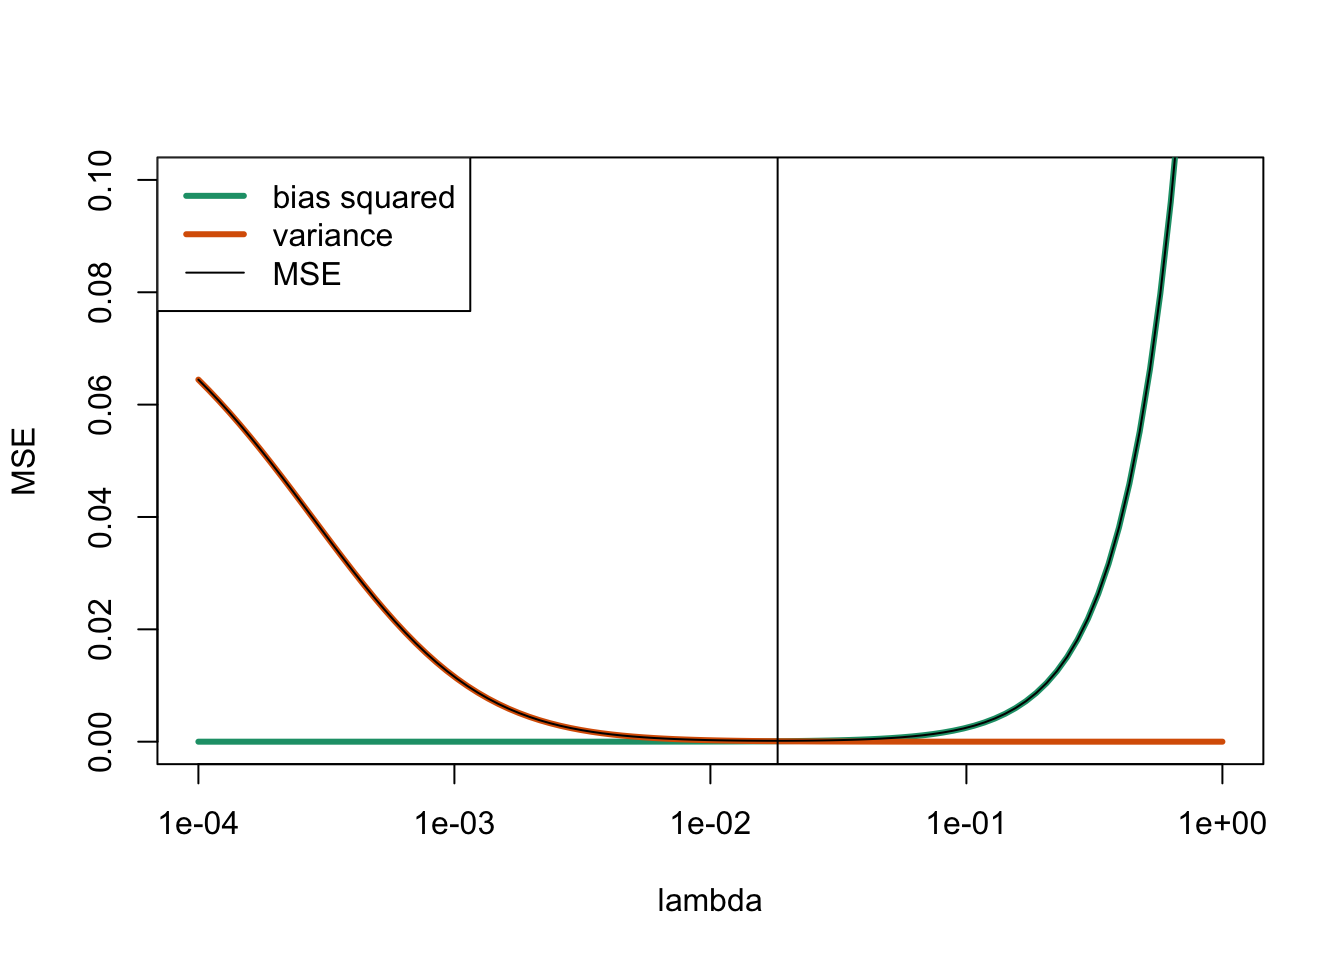
\includegraphics{MATH3714_files/figure-latex/ridge-MSE-1.pdf}

The vertical line at \(\lambda = 0.0183\)
marks the optimal value of \(\lambda\). We can see that for small \(\lambda\) the
MSE is dominated by the variance, whereas for large \(\lambda\) the main
contribution is from the bias.
\end{example}

\hypertarget{standardisation}{%
\subsection{Standardisation}\label{standardisation}}

While ridge regression can be applied directly to the original data, the
penalty is only comparable between the components of \(\beta\), if the components
have similar magnitude. Also, we do not want a method which is depends on the
units in which the \(x\) variables are measured. To address these issues, it is
common practice to first standardise each of the \(x\). In this way the
penalty will apply equally to all of the coefficients, and the results can be
transformed back to obtain \(\hat{y}\) on the original scale.

We standardise every column of the input separately: For
the input variable \(x_j\), where \(j\in\{1, \ldots, p\}\), we get
\begin{equation*}
  w_{ij}
  := \frac{x_{ij} - \overline{x_j}}{\mathrm{s}_{x_j}},
\end{equation*}
for all \(i \in \{1, \ldots, n\}\).
where \(\overline{x_j} = \frac1n \sum_{i=1}^n x_{ij}\) and
\begin{equation*}
  \mathrm{s}_{x_j}^2
  = \frac{1}{n-1} \sum_{i=1}^n (x_{ij} - \overline{x_j})^2
\end{equation*}
is the sample variance. We similarly standardise the outputs:
\begin{equation*}
  z_i
  := \frac{y_i - \overline{y}}{\mathrm{s}_y},
\end{equation*}
where \(\overline{y}\) and \(\mathrm{s}_y\) are the mean and standard
deviation of the \(y_i\). If we denote the regression coefficients
for the transformed data by \(\gamma\), then the residual sum of
squares for the transformed data is
\begin{equation*}
  r_\mathrm{tfm}(\gamma)
  = \sum_{i=1}^n \bigl(y_i - \gamma_0 - \gamma_1 w_{i1} - \cdots - \gamma_p w_{ip} \bigr)^2.
\end{equation*}

The transformed inputs satisfy
\begin{equation*}
  \sum_{i=1}^n w_{ij} = 0
\end{equation*}
for all \(j\in\{1, \ldots, p\}\) and a similar relation holds for the output.
Using these relations we find
\begin{align*}
  r_\mathrm{tfm}(\gamma)
  &= \sum_{i=1}^n \Bigl(
      \bigl( y_i - \gamma_1 w_{i1} - \cdots - \gamma_p w_{ip} \bigr)^2 \Bigr. \\
    &\hskip2cm \Bigl.
      - 2 \gamma_0 \bigl( y_i - \gamma_1 w_{i1} - \cdots - \gamma_p w_{ip} \bigr)
      + \gamma_0^2
    \Bigr) \\
  &= \sum_{i=1}^n
      \bigl( y_i - \gamma_1 w_{i1} - \cdots - \gamma_p w_{ip} \bigr)^2 \\
    &\hskip2cm
      - 2 \gamma_0 \sum_{i=1}^n \bigl( y_i - \gamma_1 w_{i1} - \cdots - \gamma_p w_{ip} \bigr)
      + n \gamma_0^2 \\
  &= \sum_{i=1}^n
      \bigl( y_i - \gamma_1 w_{i1} - \cdots - \gamma_p w_{ip} \bigr)^2 \\
    &\hskip2cm
      - 2 \gamma_0 \Bigl( \sum_{i=1}^n y_i - \gamma_1 \sum_{i=1}^n w_{i1} - \cdots - \gamma_p \sum_{i=1}^n w_{ip} \Bigr)
      + n \gamma_0^2 \\
  &= \sum_{i=1}^n
      \bigl( y_i - \gamma_1 w_{i1} - \cdots - \gamma_p w_{ip} \bigr)^2
      + n \gamma_0^2.
\end{align*}
Thus, the coefficient for the intercept can be minimised separately and
the optimal value is always~\(\gamma_0 = 0\). For this reason we do
not include the intercept in our model for the standardised data.
The design matrix is thus
\begin{equation*}
  W
  = \begin{pmatrix}
    w_{1,1} & \cdots & w_{1,p} \\
    w_{2,1} & \cdots & w_{2,p} \\
    \vdots & \ddots & \vdots \\
    w_{n,1} & \cdots & w_{n,p}
  \end{pmatrix} \in \mathbb{R}^{n\times p},
\end{equation*}
and the reduced coefficient vector is \(\gamma \in \mathbb{R}^p\).
The least squares estimator for the transformed data is then given by
\begin{equation*}
  \hat\gamma
  = (W^\top W)^{-1} W^\top z
\end{equation*}
and the ridge regression estimate is given by
\begin{equation*}
  \hat\gamma^{(\lambda)}
  = (W^\top W + \lambda I)^{-1} W^\top z.
\end{equation*}

To transform back regression estimates obtained for the transformed data,
we need to revert the standardisation: we have
\begin{equation*}
  x_{ij}
  = \mathrm{s}_{x_j} w_{ij} + \overline{x_j}
\end{equation*}
and
\begin{equation*}
  y_i
  = \mathrm{s}_y z_i + \overline{y}.
\end{equation*}
To obtain fitted values for an input \((\tilde x_1, \ldots, \tilde x_p)\)
we have to first transform these inputs:
\(\tilde w_j = (\tilde x_j - \overline{x_j}) / \mathrm{s}_{x_j}\).
Note that the mean and standard deviation come from the data used to fit
the model, and are not computed from the \(\tilde x_i\).
We then find the model mean for the transformed data:
\begin{align*}
  \hat z
  &= \sum_{j=1}^p \hat\gamma_j \tilde w_j \\
  &= \sum_{j=1}^p \hat\gamma_j \frac{\tilde x_j - \overline{x_j}}{\mathrm{s}_{x_j}} \\
  &= - \sum_{k=1}^p \frac{1}{\mathrm{s}_{x_k}} \hat\gamma_k \overline{x_k}
    + \sum_{j=1}^p \frac{1}{\mathrm{s}_{x_j}} \hat\gamma_j \tilde x_j.
\end{align*}
Finally, transforming back the response we get
\begin{align*}
  \hat y
  &= \bigl( \overline{y} - \sum_{k=1}^p \frac{\mathrm{s}_y}{\mathrm{s}_{x_k}} \hat\gamma_k \overline{x_k} \bigr)
    + \sum_{j=1}^p \frac{\mathrm{s}_y}{\mathrm{s}_{x_j}} \hat\gamma_j \tilde x_j \\
  &= \hat\beta_0 + \sum_{j=1}^p \hat\beta_j \tilde x_j,
\end{align*}
where
\begin{equation*}
  \hat\beta_j
  = \frac{\mathrm{s}_y}{\mathrm{s}_{x_j}} \hat\gamma_j
\end{equation*}
for all \(j \in \{1, \ldots, p\}\) and
\begin{equation*}
  \hat\beta_0
  = \overline{y} - \sum_{k=1}^p \frac{\mathrm{s}_y}{\mathrm{s}_{x_k}} \hat\gamma_k \overline{x_k}
  = \overline{y} - \sum_{k=1}^p \hat\beta_k \overline{x_k}.
\end{equation*}
This transformation can be used both for least squares regression
and ridge regression estimates.

\textbf{Summary}

\begin{itemize}
\tightlist
\item
  Ridge regression is an alternative estimator for the regression coefficients.
\item
  The method is useful when multicollinearity is present.
\item
  Often it is advantageous to standardise the data before performing
  ridge regression.
\end{itemize}

\clearpage

\hypertarget{S13-models}{%
\section{Model selection}\label{S13-models}}

The aim of linear regression is to find a model with the following
properties:

\begin{enumerate}
\def\labelenumi{\arabic{enumi}.}
\tightlist
\item
  The model gives good predictions \(\hat y\).
\item
  The model is easy to interpret.
\item
  The modelling assumptions are satisfied.
\end{enumerate}

These three aims can sometimes contradict: models with fewer parameters
are often easier to interpret, whereas good predictions sometimes require
a large number of parameters. Some trade-off
between these constraints must be made. In this section we discuss how
to choose the inputs for a model in a systematic way.

\hypertarget{candidates-models}{%
\subsection{Candidates Models}\label{candidates-models}}

Here we assume that we are given data with input variables \(x_1, \ldots, x_p\).
The standard model which we have discussed so far adds an intercept to these
inputs, so that there are \(p+1\) model parameters in total. We can modify
this model in various ways:

\begin{itemize}
\item
  When we discussed hypothesis tests, we allowed for the possibility that
  some inputs do not influence the output. A reasonable approach would
  be to fit a model with these inputs omitted. Since each input
  may either be included in or excluded from the model, independent of
  the others, and similarly the intercept may be included or not,
  there are \(2^{p+1}\) possible models to consider.
\item
  In the section about \protect\hyperlink{S11-improving}{Improving the Model Fit} we have seen that
  sometimes it is useful to transform input variables before using them
  in the model. This can either happen individually, \emph{e.g.}~\(x_2' = \log x_2\), or collectively, \emph{e.g.}~\(x^\ast = x_1 x_2\). The number of
  models we may obtain in this way is unlimited.
\end{itemize}

If we want to compare these candidate models in a systematic way,
we need to use efficient methods for comparison, since a often a large
number of models needs to be considered.

\hypertarget{misspecified-models}{%
\subsection{Misspecified Models}\label{misspecified-models}}

The model is said to be \textbf{misspecified}, if the data we are using
comes from a different model than the one we use to estimate
the coefficients.

\hypertarget{missing-variables}{%
\subsubsection{Missing Variables}\label{missing-variables}}

Assume that the data comes from the model
\begin{equation*}
  Y = \beta_1 x_1 + \beta_2 x_2 + \cdots + \beta_p x_p + \varepsilon,
\end{equation*}
(we can include the intercept as \(x_1 = 1\) if needed),
but we are only using the first \(q\) variables \(x_1, \ldots, x_q\),
where \(q < p\), to estimate the coefficients. Then the least squares
estimate of \(\beta = (\beta_1, \ldots, \beta_q)\) is given by
\begin{equation*}
  \hat\beta
  = (X^\top X)^{-1} X^\top y
\end{equation*}
where \(X \in \mathbb{R}^{n\times q}\),
and our estimate for the error variance \(\sigma^2\) is
\begin{equation*}
  \hat\sigma^2
  = \frac{1}{n-q} y^\top (I - H) y,
\end{equation*}
where \(H = X (X^\top X)^{-1} X^\top\) is the hat matrix computed
without using \(x_{q+1}, \ldots, x_p\).

If we write \(\tilde X \in \mathbb{R}^{n\times (p-q)}\) for the matrix with columns
\(x_{q+1}, \ldots, x_p\) and \(\tilde\beta = (\beta_{q+1}, \ldots, \beta_p) \in \mathbb{R}^{p-q}\), then the full model can be written as
\begin{equation*}
  Y
  = X \beta + \tilde X \tilde\beta + \varepsilon
\end{equation*}
and we get
\begin{align*}
  \hat\beta
  &= (X^\top X)^{-1} X^\top Y \\
  &= (X^\top X)^{-1} X^\top (X \beta + \tilde X \tilde\beta + \varepsilon) \\
  &= (X^\top X)^{-1} X^\top X \beta + (X^\top X)^{-1} X^\top \tilde X \tilde\beta + (X^\top X)^{-1} X^\top \varepsilon\\
  &= \beta + (X^\top X)^{-1} X^\top \tilde X \tilde\beta + (X^\top X)^{-1} X^\top \varepsilon.
\end{align*}
Thus, we have
\begin{equation*}
  \mathbb{E}(\hat\beta)
  = \beta + (X^\top X)^{-1} X^\top \tilde X \tilde\beta
\end{equation*}
and
\begin{equation*}
  \mathop{\mathrm{bias}}(\hat\beta)
  = (X^\top X)^{-1} X^\top \tilde X \tilde\beta.
\end{equation*}
This shows that now the estimate is biased in general. There are two
special cases when omitting variables does not introduce a bias:
The first is when all of the omitted coefficients equal zero, \emph{i.e.}~when
we have \(\tilde\beta = 0\). The second case is when the omitted inputs are
orthogonal to the included inputs, since then we have \(X^\top \tilde X = 0\).

Using the formula for \(\hat\beta\) we find
\begin{align*}
  \mathop{\mathrm{Cov}}( \hat\beta )
  &= \mathop{\mathrm{Cov}}\Bigl( \beta + (X^\top X)^{-1} X^\top \tilde X \tilde\beta + (X^\top X)^{-1} X^\top \varepsilon\Bigr) \\
  &= \mathop{\mathrm{Cov}}\Bigl( (X^\top X)^{-1} X^\top \varepsilon\Bigr) \\
  &= \sigma^2 (X^\top X)^{-1} X^\top I X (X^\top X)^{-1} \\
  &= \sigma^2 (X^\top X)^{-1}.
\end{align*}
Similar to our derivation in the section \protect\hyperlink{var-est-bias}{Estimating the Error Variance}
one can show that
\begin{equation*}
  \mathbb{E}\bigl( \hat\sigma^2 \bigr)
  = \sigma^2 + \frac{\tilde\beta^\top \tilde X^\top (I - H) \tilde X \tilde \beta}{n-q}.
\end{equation*}
This shows that the estimate of the error variance is in general also biased.

This shows that our estimates can become biased if some of the inputs
are missing from our model. As in the previous section, it may happen
that the MSE of the parameter estimates in the reduced model
is smaller than the MSE in the correct model; this is the case if the
variance of the estimates decreases enough to compensate for the
introduced bias.

\hypertarget{unnecessary-variables}{%
\subsubsection{Unnecessary Variables}\label{unnecessary-variables}}

If the data comes from a model with fewer inputs than the ones we are using,
the model is not ``misspecified'' in the strict sense. It is just the case that
some of the true \(\beta_j\) exactly equal zero. In this case, our previous
results show that the least squares estimate is unbiased.

Including additional variables into a model still can cause problems:
One can show that each unnecessary variable added increases the variance of the
estimates \(\hat\beta_j\). Instead of giving a proof of this fact,
we illustrate the effect using a numerical example.

\begin{example}
Here we consider the \texttt{stackloss} data set with an added column of
noise. We have see that
\begin{equation*}
  \mathop{\mathrm{Var}}( \hat\beta_j )
  = \sigma^2 \bigl( X^\top X \bigr)^{-1}_{jj}.
\end{equation*}
While we don't know the true value of \(\sigma^2\), we can determine
the relative change in variance when adding a column, since this process
does not change \(\sigma^2\) and thus \(\sigma^2\) will cancel when we
determine the relative change in variance.

We first compute the diagonal elements of \(\bigl( X^\top X \bigr)^{-1}\)
for the original dataset:

\begin{Shaded}
\begin{Highlighting}[]
\NormalTok{X1 }\OtherTok{\textless{}{-}} \FunctionTok{model.matrix}\NormalTok{(stack.loss }\SpecialCharTok{\textasciitilde{}}\NormalTok{ ., }\AttributeTok{data =}\NormalTok{ stackloss)}
\NormalTok{d1 }\OtherTok{\textless{}{-}} \FunctionTok{diag}\NormalTok{(}\FunctionTok{solve}\NormalTok{(}\FunctionTok{t}\NormalTok{(X1) }\SpecialCharTok{\%*\%}\NormalTok{ X1))}
\NormalTok{d1}
\end{Highlighting}
\end{Shaded}

\begin{Shaded}
\begin{Highlighting}[]
\NormalTok{\#  (Intercept)     Air.Flow   Water.Temp   Acid.Conc. }
\NormalTok{\# 13.452726695  0.001728874  0.012875424  0.002322167}
\end{Highlighting}
\end{Shaded}

Now we add a column of noise and re-compute the values:

\begin{Shaded}
\begin{Highlighting}[]
\FunctionTok{set.seed}\NormalTok{(}\DecValTok{20211115}\NormalTok{)}
\NormalTok{n }\OtherTok{\textless{}{-}} \FunctionTok{nrow}\NormalTok{(X1)}
\NormalTok{X2 }\OtherTok{\textless{}{-}} \FunctionTok{cbind}\NormalTok{(X1, }\FunctionTok{rnorm}\NormalTok{(n))}
\NormalTok{d2 }\OtherTok{\textless{}{-}} \FunctionTok{diag}\NormalTok{(}\FunctionTok{solve}\NormalTok{(}\FunctionTok{t}\NormalTok{(X2) }\SpecialCharTok{\%*\%}\NormalTok{ X2))}
\NormalTok{d2}
\end{Highlighting}
\end{Shaded}

\begin{Shaded}
\begin{Highlighting}[]
\NormalTok{\#  (Intercept)     Air.Flow   Water.Temp   Acid.Conc.              }
\NormalTok{\# 14.397515774  0.001730570  0.015195467  0.002796487  0.064828744}
\end{Highlighting}
\end{Shaded}

Finally, we determine the change in variance in percent:

\begin{Shaded}
\begin{Highlighting}[]
\FunctionTok{round}\NormalTok{(}\DecValTok{100} \SpecialCharTok{*}\NormalTok{ (d2[}\SpecialCharTok{{-}}\DecValTok{5}\NormalTok{] }\SpecialCharTok{{-}}\NormalTok{ d1) }\SpecialCharTok{/}\NormalTok{ d1, }\DecValTok{3}\NormalTok{)}
\end{Highlighting}
\end{Shaded}

\begin{Shaded}
\begin{Highlighting}[]
\NormalTok{\# (Intercept)    Air.Flow  Water.Temp  Acid.Conc. }
\NormalTok{\#       7.023       0.098      18.019      20.426}
\end{Highlighting}
\end{Shaded}

We see that the variances of the \(\hat\beta_j\) increased by up to \(20\%\)
when we added the unnecessary input.
\end{example}

The example illustrates that it is important to keep the model as small
as possible.

\hypertarget{criteria}{%
\subsection{Assessing Models}\label{criteria}}

A variety of criteria is used in practice to select variables to include
in a regression model.

\begin{enumerate}
\def\labelenumi{\arabic{enumi}.}
\item
  The \protect\hyperlink{def:R-squared}{coefficient of multiple determination}, \(R^2\), can be used
  to compare models. ``Good'' models have large \(R^2\).
  If comparisons are made between models with different
  numbers of inputs then the \protect\hyperlink{def:adjusted-R-squared}{adjusted \(R^2\)-value},
  \(R^2_\mathrm{adj}\), must be used.
\item
  The estimate for the error variance,
  \begin{equation*}
   \hat\sigma^2 = \frac{1}{n - q} \sum_{i=1}^n (y_i - \hat y_i)^2
    \end{equation*}
  can be used, where \(q\) is the number of columns of the design matrix.
  (For the full model with an intercept we have \(q = p+1\).)
  ``Good'' models have small \(\hat\sigma^2\). Since
  \begin{align*}
   R^2_\mathrm{adj}
   &= 1 - \frac{\frac{1}{n-q}\mathrm{s}_{\hat\varepsilon}^2}{\frac{1}{n-1}\mathrm{s}_y^2} \\
   &= 1 - \frac{\frac{n-1}{n-q}\mathrm{s}_{\hat\varepsilon}^2}{\mathrm{s}_y^2} \\
   &= 1 - \frac{\frac{1}{n-q} \sum_{i=1}^n (y_i - \hat y_i)^2}{\mathrm{s}_y^2} \\
   &= 1 - \frac{\hat\sigma^2}{\mathrm{s}_y^2},
    \end{align*}
  where \(\mathrm{s}_{\hat\varepsilon}^2\) and \(\mathrm{s}_y^2\) are the sample variances
  as before, minimising \(\hat\sigma^2\) is equivalent to
  maximising \(R^2_\mathrm{adj}\). Thus, this criterion is equivalent to
  the first one.
\item
  The \textbf{Prediction Error Sum of Squares (PRESS)} compares each
  output \(y_i\) to the fitted value \(\hat y^{(i)}_i\) for observation i,
  computed without using sample~\(i\):
  \begin{equation*}
    \mathrm{PRESS}
    := \sum_{i=1}^n \bigl( y_i - \hat y^{(i)}_i \bigr)^2.
  \end{equation*}
  In the comparison, \(\hat y^{(i)}_i\) is used instead of \(\hat y_i\)
  so that in models with too many parameters, overfitting does not
  result in overoptimistic estimates.
  ``Good'' models have small PRESS. The following lemma helps to compute
  PRESS without having to fit \(n\) separate models.

  \begin{lemma}
  \protect\hypertarget{lem:PRESS}{}\label{lem:PRESS}We have
  \begin{equation*}
    \mathrm{PRESS}
    = \sum_{i=1}^n \Bigl( \frac{\hat\varepsilon_i}{1 - h_{ii}} \Bigr)^2,
  \end{equation*}
  where \(h_{ii}\) denotes the diagonal elements of the hat matrix~\(H\).
  \end{lemma}

  \begin{proof}
  From equation~\eqref{eq:dbeta-i} we know how the estimated regression
  coefficients change, when observation \(i\) is deleted from the model:
  \begin{equation*}
    \hat\beta^{(i)} - \hat\beta
    = - (X^\top X)^{-1} x_i \frac{\hat\varepsilon_i}{1 - h_{ii}}.
  \end{equation*}
  Thus we have
  \begin{align*}
    \hat y^{(i)}_i - \hat y_i
    &= \bigl( X \hat\beta^{(i)} - X \hat\beta \bigr)_i \\
    &= - \bigl( X (X^\top X)^{-1} x_i \frac{\hat\varepsilon_i}{1 - h_{ii}} \bigr)_i \\
    &= - x_i^\top (X^\top X)^{-1} x_i \frac{\hat\varepsilon_i}{1 - h_{ii}} \\
    &= - \frac{h_{ii}}{1 - h_{ii}} \hat\varepsilon_i.
  \end{align*}
  From this we get
  \begin{align*}
    y_i - \hat y^{(i)}_i
    &= y_i - \hat y_i + \hat y_i - \hat y^{(i)}_i \\
    &= \hat\varepsilon_i + \frac{h_{ii}}{1 - h_{ii}} \hat\varepsilon_i \\
    &= \frac{1}{1 - h_{ii}} \hat\varepsilon_i.
  \end{align*}
  Substituting this expression into the definition of PRESS
  completes the proof.
  \end{proof}
\item
  We can consider
  \begin{equation*}
    C_q
    := \frac{1}{\hat{\sigma}^2} \sum_{i=1}^n (y_i - \hat y_i)^2 - n + 2q.
  \end{equation*}
  The subscript \(q\) in \(C_q\) denotes the number of parameters in the model.
  This quantity is called \textbf{Mallows' Cp} or sometimes
  \textbf{Mallows' Ck}. ``Good'' models have \(C_q \approx q\).

  The form of \(C_q\) is explained by the fact that it approximates the
  quantity
  \begin{equation*}
    \Gamma_q
    := \frac{1}{\sigma^2} \sum_{i=1}^n \mathop{\mathrm{MSE}}\nolimits(\hat y_i).
  \end{equation*}
  To see that \(C_q \approx \Gamma_q\) we first rewrite \(\Gamma_q\) as
  \begin{align*}
    \Gamma_q
    &= \sum_{i=1}^n \Bigl( \mathop{\mathrm{Var}}(\hat y_i) + \mathop{\mathrm{bias}}(\hat y_i)^2 \Bigr) \\
    &= \frac{1}{\sigma^2} \sum_{i=1}^n \mathop{\mathrm{bias}}(\hat y_i)^2 + \frac{1}{\sigma^2} \sum_{i=1}^n \mathop{\mathrm{Var}}(\hat y_i).
  \end{align*}
  Since \(\hat y = HY \sim \mathcal{N}(HX\beta, \sigma^2 HIH^\top) = \mathcal{N}(X\beta, \sigma^2 H)\) we have \(\mathop{\mathrm{Var}}(\hat y_i) = \sigma^2 h_{ii}\) were \(h_{ii}\) are
  the diagonal elements of the hat matrix. Furthermore, using the trace
  operator (see appendix~\ref{trace}) we find
  \begin{align*}
    \sum_{i=1}^n h_{ii}
    &= \mathop{\mathrm{tr}}(H) \\
    &= \mathop{\mathrm{tr}}\bigl(X (X^\top X)^{-1} X^\top \bigr) \\
    &= \mathop{\mathrm{tr}}\bigl((X^\top X)^{-1} X^\top X \bigr) \\
    &= \mathop{\mathrm{tr}}(I) \\
    &= q,
  \end{align*}
  and thus
  \begin{equation}
    \Gamma_q
    = \frac{1}{\sigma^2} \sum_{i=1}^n \mathop{\mathrm{bias}}(\hat y_i)^2 + q.  \label{eq:Gamma-q}
  \end{equation}
  This shows that for a model where the \(\hat y_i\) are unbiased,
  we have \(\Gamma_q = q\), and if there is a bias we have \(\Gamma_q > q\).
  We now show that \(C_q \approx \Gamma_q\).

  We also have \(\hat y = \mathop{\mathrm{bias}}(\hat y) + HY\) and thus
  \begin{equation*}
    Y - \hat y
    = (I - H)Y - \mathop{\mathrm{bias}}(\hat y)
    = (I - H) \varepsilon- \mathop{\mathrm{bias}}(\hat y).
  \end{equation*}
  Using this relation, one can show that
  \begin{align*}
    \mathbb{E}\Bigl( \sum_{i=1}^n (y_i - \hat y_i)^2 \Bigr)
    &= (Y - \hat y)^\top (Y - \hat y) \\
    &= \dots \\
    &= \sum_{i=1}^n \mathop{\mathrm{bias}}(\hat y_i)^2 + (n-q) \sigma^2.
  \end{align*}
  Substituting this result into the formula for \(\Gamma_q\) we get
  \begin{align*}
    \Gamma_q
    &= \frac{1}{\sigma^2} \mathbb{E}\Bigl( \sum_{i=1}^n (y_i - \hat y_i)^2 \Bigr)
        - (n-q)
        + q \\
    &\approx \frac{1}{\sigma^2} \sum_{i=1}^n (y_i - \hat y_i)^2 - n + 2q \\
    &\approx \frac{1}{\hat\sigma^2} \sum_{i=1}^n (y_i - \hat y_i)^2 - n + 2q \\
    &= C_q.
  \end{align*}

  A plot of \(C_q\) \emph{vs.}~\(q\) will show adequate models as points
  close to the line \(C_q=q\). Points far from the line are not recommended,
  and, of those which lie close to the line, we generally prefer smaller
  models. The method relies on having a good estimate of~\(\sigma^2\).
\item
  \textbf{Akaike's Information Criterion (AIC)} is defined as
  \begin{equation*}
    \mathrm{AIC}
    = 2q - 2 \log(\hat L),
  \end{equation*}
  where \(q\) is the number of parameters in the model, and \(\hat L\)
  is the maximum of the likelihood function when these \(q\) parameters
  are chosen optimally. ``Good'' models have small AIC.

  Since we assume \(\varepsilon_i \sim \mathcal{N}(0, \sigma^2)\), i.i.d. and
  we have \(\varepsilon_i = y_i - x_i^\top\beta\), the likelihood function
  for our model is
  \begin{align*}
    L(\beta, \sigma^2; X, y)
    &= \prod_{i=1}^n \frac{1}{\sqrt{2\pi\sigma^2}} \exp\Bigl( - \frac{(y_i - x_i^\top\beta)^2}{2\sigma^2} \Bigr) \\
    &= \frac{1}{(2\pi\sigma^2)^{n/2}} \exp\Bigl( - \sum_{i=1}^n \frac{(y_i - x_i^\top\beta)^2}{2\sigma^2} \Bigr).
  \end{align*}
  Taking logarithms we get
  \begin{align*}
    \log L(\beta, \sigma^2; X, y)
    &= -\frac{n}{2} \log(2\pi\sigma^2) - \sum_{i=1}^n \frac{(y_i - x_i^\top\beta)^2}{2\sigma^2} \\
    &= -\frac{n}{2} \log(2\pi\sigma^2) - \frac{1}{2\sigma^2} r(\beta),
  \end{align*}
  where \(r(\beta)\) is the residual sum of squares, as introduced
  in the section about \protect\hyperlink{S02-multiple}{Least Squares Estimates}. To compute the AIC
  we need to maximise this expression. The values of \(\beta\) and \(\sigma^2\)
  where the maximum is taken are called the \textbf{maximum likelihood estimate (MLE)}
  for \(\beta\) and \(\sigma^2\). From lemma~\ref{lem:multiple-LSQ} we know
  that for fixed \(\sigma^2\), \(L\) takes its maximum when \(\beta\) equals the
  least squares estimate \(\hat\beta\). Taking derivatives we can then
  find the optimal value of \(\sigma^2\). The result is
  \begin{equation*}
    \hat\sigma^2_\mathrm{MLE}
    = \frac1n r(\hat\beta)
    = \frac{1}{n} \sum_{i=1}^n (y_i - x_i^\top \hat\beta)^2
    = \frac{n-q}{n} \hat\sigma^2.
  \end{equation*}
  Thus we get
  \begin{align*}
    \mathrm{AIC}
    &= 2q + n \log(2\pi\hat\sigma^2_\mathrm{MLE}) + \frac{1}{\hat\sigma^2_\mathrm{MLE}} r(\hat\beta) \\
    &= 2q + n \log\bigl( 2\pi r(\hat\beta) / n \bigr) + n \\
    &= 2q + n \log\bigl( \|\hat\varepsilon\|^2 \bigr) + n + n \log( 2\pi / n )
  \end{align*}
\end{enumerate}

\textbf{Summary}

\begin{itemize}
\tightlist
\item
  We have discussed how different models can be considered by omitting
  existing variables or by adding non-linear functions of the inputs
  as new variables.
\item
  We have seen that removing too many variables can introduce a bias.
\item
  We have seen that adding too many variables can increase the variance
  of the estimate.
\item
  We have considered different criteria for choosing the ``best'' model.
\end{itemize}

\clearpage

\hypertarget{P04}{%
\section*{Problem Sheet 4}\label{P04}}
\addcontentsline{toc}{section}{Problem Sheet 4}

\excludecomment{myanswers}

You should attempt all these questions and write up your solutions in advance
of your workshop in week~9 where the answers will be discussed.

\textbf{13} Consider the data set \texttt{pressure}, built into~R, which
describes the vapour pressure~\(P\) of mercury as a function of
temperature~\(T\).

\begin{enumerate}
\def\labelenumi{\alph{enumi}.}
\tightlist
\item
  For given \(T_0\), explain how a model of the form
  \(P = \beta_0 + T \beta_1 + \max(0, T-T_0) \beta_2 + \varepsilon\) can be
  fitted to the data.
\end{enumerate}

\begin{myanswers}

We can fit a model with an intercept and two inputs,
\(T\) and \(\max(0, T-T_0)\). In R we can use the following
commands to fit such a model:

\begin{Shaded}
\begin{Highlighting}[]
\NormalTok{T0 }\OtherTok{\textless{}{-}}\NormalTok{ the.given.value }\CommentTok{\# substitute the value of T0 here}
\NormalTok{m }\OtherTok{\textless{}{-}} \FunctionTok{lm}\NormalTok{(pressure }\SpecialCharTok{\textasciitilde{}}\NormalTok{ temperature }\SpecialCharTok{+} \FunctionTok{I}\NormalTok{(}\FunctionTok{pmax}\NormalTok{(}\DecValTok{0}\NormalTok{, temperature}\SpecialCharTok{{-}}\NormalTok{T0)),}
        \AttributeTok{data =}\NormalTok{ pressure)}
\end{Highlighting}
\end{Shaded}

\end{myanswers}

\begin{enumerate}
\def\labelenumi{\alph{enumi}.}
\setcounter{enumi}{1}
\tightlist
\item
  Why might a model of this form make sense for the given data?
\end{enumerate}

\begin{myanswers}
Such a model may make sense, because the slope of the
samples increases faster than linear as the temperature~\(T\)
increases. The term \(\max(0, T-T_0)\) is zero for small~\(T\),
but adds an additional slope once \(T\) exceeds the cutoff
temperature~\(T_0\).

\end{myanswers}

\begin{enumerate}
\def\labelenumi{\alph{enumi}.}
\setcounter{enumi}{2}
\tightlist
\item
  What is a good value of \(T_0\) for this data set?
\end{enumerate}

\begin{myanswers}
\(T_0\) should be placed at the end of the ``flat'' part
of the plot, where the pressure starts increasing more
quickly. A quick experiment shows that the best \(R^2\)
value is achieved for \(T_0 \approx 273\):

\begin{Shaded}
\begin{Highlighting}[]
\NormalTok{T0 }\OtherTok{\textless{}{-}} \DecValTok{273}
\NormalTok{m }\OtherTok{\textless{}{-}} \FunctionTok{lm}\NormalTok{(pressure }\SpecialCharTok{\textasciitilde{}}\NormalTok{ temperature }\SpecialCharTok{+} \FunctionTok{I}\NormalTok{(}\FunctionTok{pmax}\NormalTok{(}\DecValTok{0}\NormalTok{, temperature }\SpecialCharTok{{-}}\NormalTok{ T0)),}
        \AttributeTok{data=}\NormalTok{pressure)}
\FunctionTok{summary}\NormalTok{(m)}
\end{Highlighting}
\end{Shaded}

\begin{Shaded}
\begin{Highlighting}[]
\NormalTok{\# }
\NormalTok{\# Call:}
\NormalTok{\# lm(formula = pressure \textasciitilde{} temperature + I(pmax(0, temperature {-} }
\NormalTok{\#     T0)), data = pressure)}
\NormalTok{\# }
\NormalTok{\# Residuals:}
\NormalTok{\#     Min      1Q  Median      3Q     Max }
\NormalTok{\# {-}53.125 {-}17.553  {-}6.308  13.017  55.839 }
\NormalTok{\# }
\NormalTok{\# Coefficients:}
\NormalTok{\#                               Estimate Std. Error t value Pr(\textgreater{}|t|)    }
\NormalTok{\# (Intercept)                  {-}17.62933   14.63735  {-}1.204   0.2459    }
\NormalTok{\# temperature                    0.25472    0.08774   2.903   0.0104 *  }
\NormalTok{\# I(pmax(0, temperature {-} T0))   7.77118    0.38024  20.437 6.85e{-}13 ***}
\NormalTok{\# {-}{-}{-}}
\NormalTok{\# Signif. codes:  0 \textquotesingle{}***\textquotesingle{} 0.001 \textquotesingle{}**\textquotesingle{} 0.01 \textquotesingle{}*\textquotesingle{} 0.05 \textquotesingle{}.\textquotesingle{} 0.1 \textquotesingle{} \textquotesingle{} 1}
\NormalTok{\# }
\NormalTok{\# Residual standard error: 29.86 on 16 degrees of freedom}
\NormalTok{\# Multiple R{-}squared:  0.9843,  Adjusted R{-}squared:  0.9823 }
\NormalTok{\# F{-}statistic: 501.3 on 2 and 16 DF,  p{-}value: 3.705e{-}15}
\end{Highlighting}
\end{Shaded}

To get a better understanding of how the extra term
\(\max(0, T-T_0)\) improves model fit, we plot the data
together with the fitted model:

\begin{Shaded}
\begin{Highlighting}[]
\FunctionTok{plot}\NormalTok{(pressure)}
\NormalTok{T.plot }\OtherTok{\textless{}{-}} \FunctionTok{seq}\NormalTok{(}\DecValTok{0}\NormalTok{, }\DecValTok{360}\NormalTok{, }\AttributeTok{l=}\DecValTok{100}\NormalTok{)}
\NormalTok{p.plot }\OtherTok{\textless{}{-}} \FunctionTok{predict}\NormalTok{(m, }\FunctionTok{data.frame}\NormalTok{(}\AttributeTok{temperature=}\NormalTok{T.plot))}
\FunctionTok{lines}\NormalTok{(T.plot, p.plot)}
\end{Highlighting}
\end{Shaded}

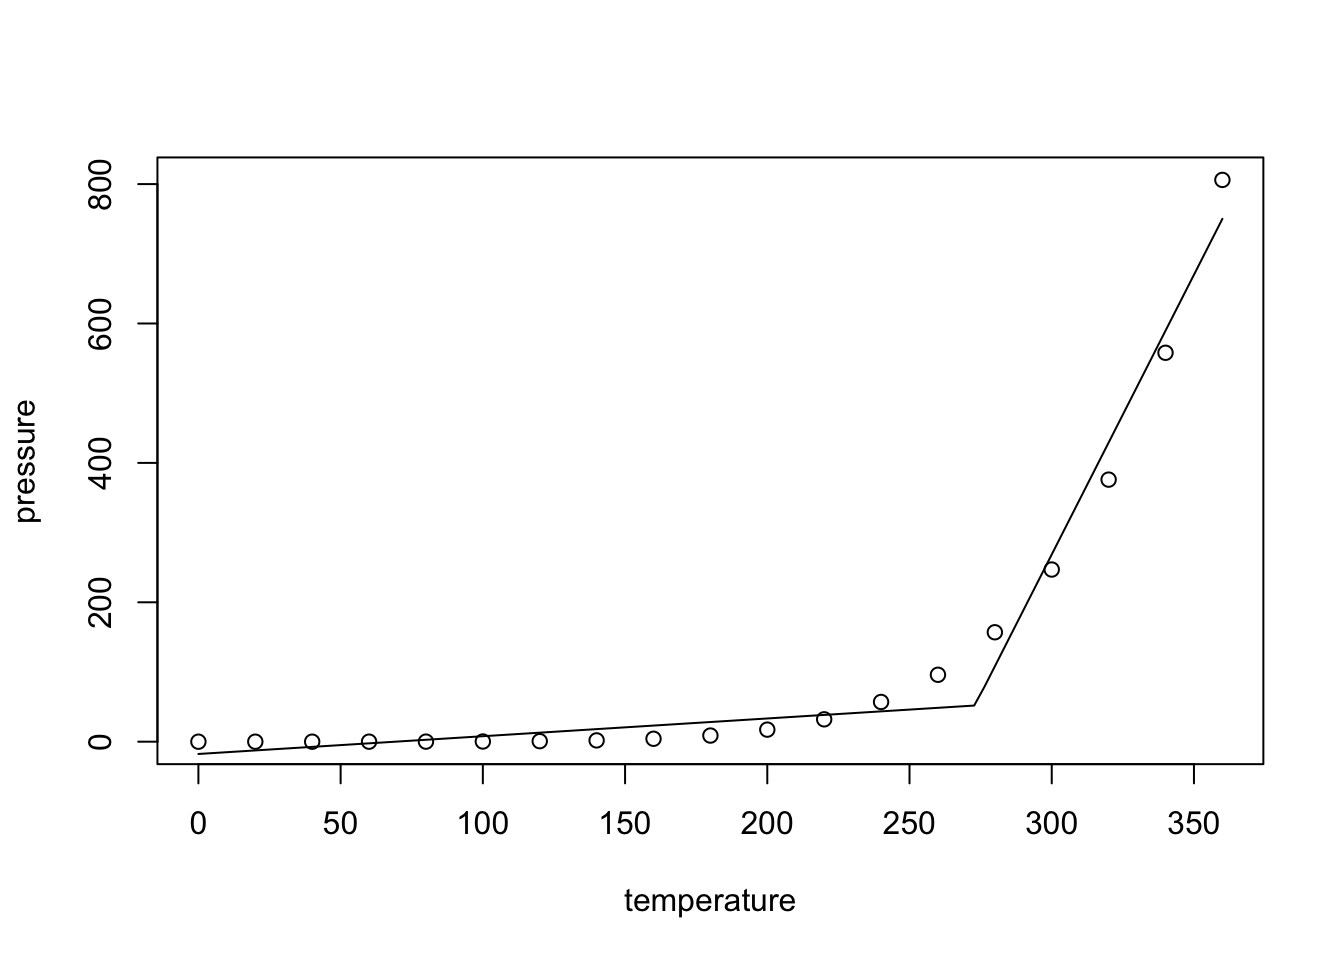
\includegraphics{MATH3714_files/figure-latex/P04Q13c-1.pdf}

As expected, for \(T > 273 = T_0\), the slope of the
fitted line increases, leading to greatly improved
model fit. (An alternative, and probably superior approach would
be to transform the data and try to fit a straight line to the
transformed data instead.)

\end{myanswers}

\textbf{14} Where possible, rewrite the following regression models in linear form.

\begin{enumerate}
\def\labelenumi{\alph{enumi}.}
\tightlist
\item
  \(y = \beta_0 \beta_1^x\)
\end{enumerate}

\begin{myanswers}
We can take logarithms:
\begin{equation*}
  \log(y)
  = \log(\beta_0) + x \log(\beta_1)
  =: \beta_0' + x \beta_1'.
\end{equation*}
Notice that writing \(\log(y) = \beta_0' + x \beta_1' + \varepsilon\)
implies \(y = \beta_0 \beta_1^x \exp(\varepsilon)\).

\end{myanswers}

\begin{enumerate}
\def\labelenumi{\alph{enumi}.}
\setcounter{enumi}{1}
\tightlist
\item
  \(y = \beta_0 + \beta_1 \sin(x_1) + \beta_2 \exp(x_2)\)
\end{enumerate}

\begin{myanswers}
We can simply set \(x_1' = \sin(x_1)\) and \(x_2' = \exp(x_2)\).
This transformation does not affect the error term.

\end{myanswers}

\begin{enumerate}
\def\labelenumi{\alph{enumi}.}
\setcounter{enumi}{2}
\tightlist
\item
  \(y = \frac{x}{\beta_0 + \beta_1 x}\)
\end{enumerate}

\begin{myanswers}
We can write
\begin{equation*}
  \frac1y
  = \frac{\beta_0 + \beta_1 x}{x}
  = \beta_0 \frac1x + \beta_1.
\end{equation*}
Thus we can use \(x' = 1/x\), \(y' = 1/y\), \(\beta_0' = \beta_1\) and
\(\beta_1' = \beta_0\). This transformation affects the noise, too,
so some care is needed.

\end{myanswers}

\textbf{15} Consider the dataset from

\begin{itemize}
\tightlist
\item
  \url{http://www1.maths.leeds.ac.uk/~voss/2021/MATH3714/P04Q14.csv}
\end{itemize}

The dataset contains samples \((x_{i,1}, x_{i,2}, y_i)\). We want to
find a model for \(y\) as a function of \(x_1\) and~\(x_2\).

\begin{enumerate}
\def\labelenumi{\alph{enumi}.}
\tightlist
\item
  Fit a linear model to the data and produce a residual plot.
  Based on the plot, discuss how well the model fits the data.
\end{enumerate}

\begin{myanswers}
We can fit the model as follows:

\begin{Shaded}
\begin{Highlighting}[]
\CommentTok{\# data from http://www1.maths.leeds.ac.uk/\textasciitilde{}voss/2021/MATH3714/P04Q14.csv}
\NormalTok{d }\OtherTok{\textless{}{-}} \FunctionTok{read.csv}\NormalTok{(}\StringTok{"data/P04Q14.csv"}\NormalTok{)}
\NormalTok{m }\OtherTok{\textless{}{-}} \FunctionTok{lm}\NormalTok{(y }\SpecialCharTok{\textasciitilde{}}\NormalTok{ x1 }\SpecialCharTok{+}\NormalTok{ x2, }\AttributeTok{data =}\NormalTok{ d)}
\FunctionTok{plot}\NormalTok{(}\FunctionTok{fitted}\NormalTok{(m), }\FunctionTok{resid}\NormalTok{(m))}
\end{Highlighting}
\end{Shaded}

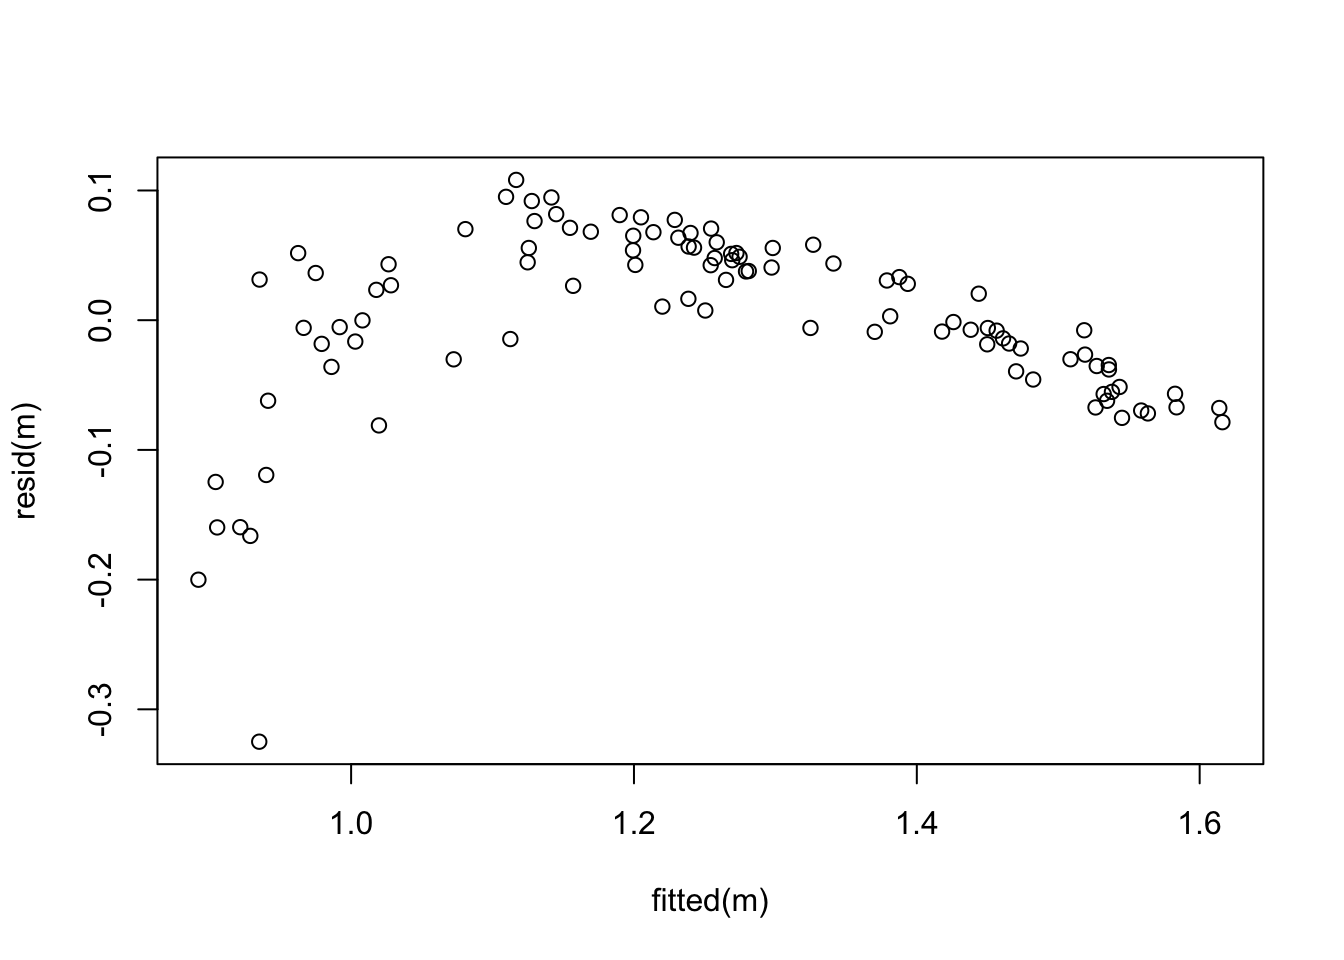
\includegraphics{MATH3714_files/figure-latex/P04Q14a-1.pdf}

The mean of the residuals does not form a straight line, so the
dependency of \(y\) on the \(x_i\) seems to be nonlinear. Also, the variance
of the residuals decreases as \(\hat y\) increases. Model fit is not good
and a transformation of the data may be useful.

\end{myanswers}

\begin{enumerate}
\def\labelenumi{\alph{enumi}.}
\setcounter{enumi}{1}
\tightlist
\item
  Apply a Power Transform to the model, as described in
  section~\ref{power-transform} of the notes. Explain your choice of \(\lambda\).
\end{enumerate}

\begin{myanswers}
To choose the exponent \(\lambda\), we plot the residual sum of squares
as a function of \(\lambda\).

\begin{Shaded}
\begin{Highlighting}[]
\NormalTok{gm }\OtherTok{\textless{}{-}} \FunctionTok{exp}\NormalTok{(}\FunctionTok{mean}\NormalTok{(}\FunctionTok{log}\NormalTok{(d}\SpecialCharTok{$}\NormalTok{y)))}
\NormalTok{lambda }\OtherTok{\textless{}{-}} \FunctionTok{seq}\NormalTok{(}\DecValTok{3}\NormalTok{, }\DecValTok{5}\NormalTok{, }\AttributeTok{length.out =} \DecValTok{101}\NormalTok{)}
\NormalTok{rss }\OtherTok{\textless{}{-}} \FunctionTok{numeric}\NormalTok{(}\FunctionTok{length}\NormalTok{(lambda))}
\ControlFlowTok{for}\NormalTok{ (i }\ControlFlowTok{in} \FunctionTok{seq\_along}\NormalTok{(lambda)) \{}
\NormalTok{    li }\OtherTok{\textless{}{-}}\NormalTok{ lambda[i]}
\NormalTok{    y.prime }\OtherTok{\textless{}{-}}\NormalTok{ (d}\SpecialCharTok{$}\NormalTok{y}\SpecialCharTok{\^{}}\NormalTok{li }\SpecialCharTok{{-}} \DecValTok{1}\NormalTok{) }\SpecialCharTok{/}\NormalTok{ (li }\SpecialCharTok{*}\NormalTok{ gm}\SpecialCharTok{\^{}}\NormalTok{(li}\DecValTok{{-}1}\NormalTok{))}
\NormalTok{    mi }\OtherTok{\textless{}{-}} \FunctionTok{lm}\NormalTok{(y.prime }\SpecialCharTok{\textasciitilde{}}\NormalTok{ x1 }\SpecialCharTok{+}\NormalTok{ x2, }\AttributeTok{data =}\NormalTok{ d)}
\NormalTok{    rss[i] }\OtherTok{\textless{}{-}} \FunctionTok{sum}\NormalTok{(}\FunctionTok{resid}\NormalTok{(mi)}\SpecialCharTok{\^{}}\DecValTok{2}\NormalTok{)}
\NormalTok{\}}
\FunctionTok{plot}\NormalTok{(lambda, rss, }\AttributeTok{type=}\StringTok{"l"}\NormalTok{)}

\NormalTok{cutoff }\OtherTok{\textless{}{-}} \FunctionTok{min}\NormalTok{(rss) }\SpecialCharTok{*}\NormalTok{ (}\DecValTok{1} \SpecialCharTok{+} \FunctionTok{qt}\NormalTok{(}\FloatTok{0.971}\NormalTok{, }\DecValTok{51}\NormalTok{)}\SpecialCharTok{\^{}}\DecValTok{2} \SpecialCharTok{/} \DecValTok{51}\NormalTok{)}
\FunctionTok{abline}\NormalTok{(}\AttributeTok{h =}\NormalTok{ cutoff)}
\end{Highlighting}
\end{Shaded}

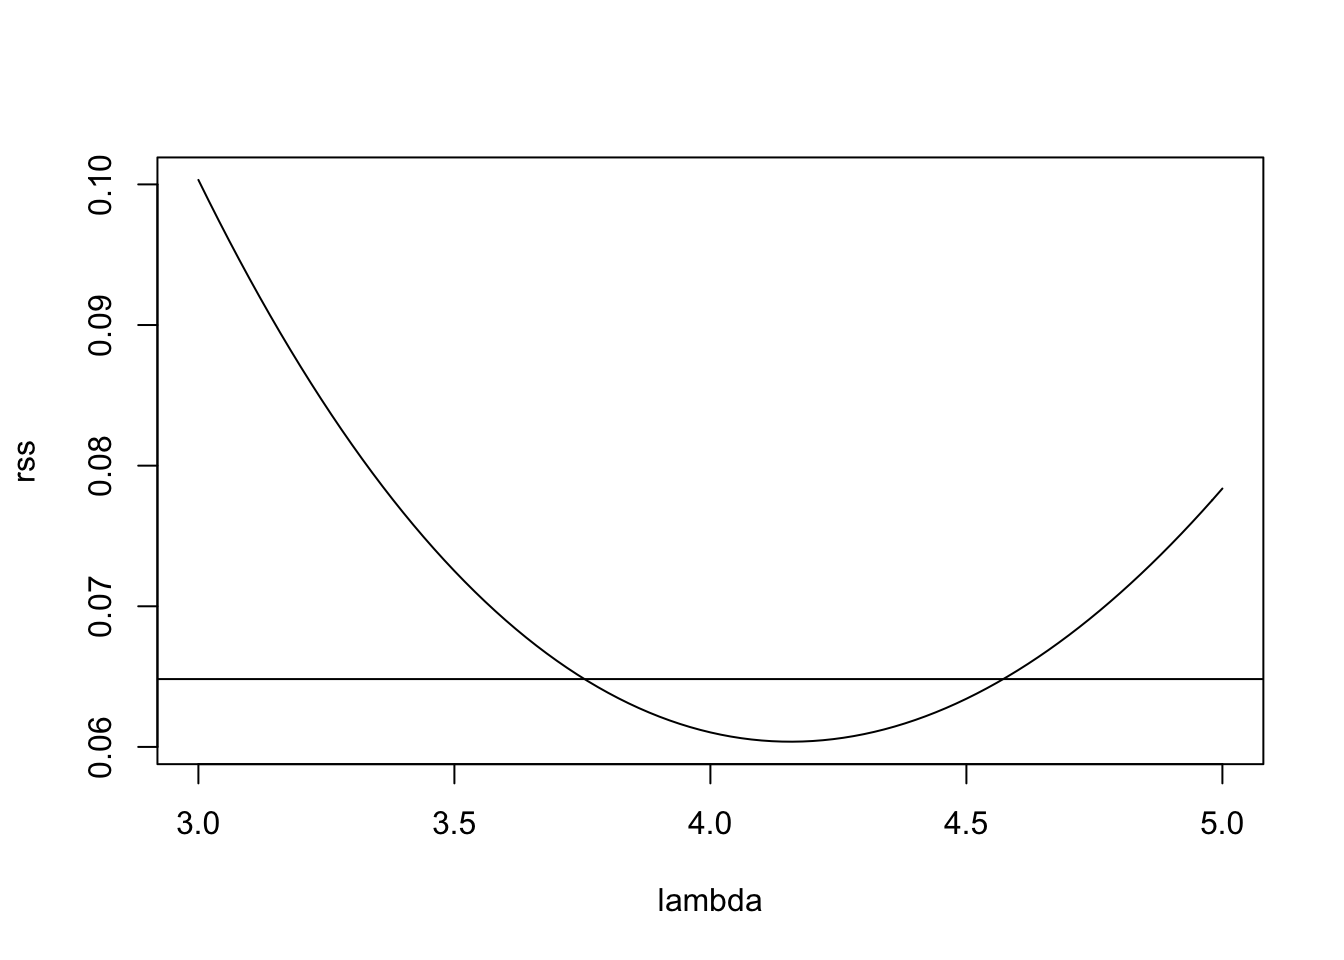
\includegraphics{MATH3714_files/figure-latex/P04Q14b-1.pdf}

The horizonal line in this plot indicates the cutoff suggested by the
rule of thumb in~\eqref{eq:power-cutoff}. Of the values of \(\lambda\)
where \texttt{rss} is below the cutoff, \(\lambda = 4\) seems the most ``simple'',
so we try this value here.

\begin{Shaded}
\begin{Highlighting}[]
\NormalTok{y.prime }\OtherTok{\textless{}{-}}\NormalTok{ d}\SpecialCharTok{$}\NormalTok{y }\SpecialCharTok{\^{}} \DecValTok{4}
\NormalTok{m }\OtherTok{\textless{}{-}} \FunctionTok{lm}\NormalTok{(y.prime }\SpecialCharTok{\textasciitilde{}}\NormalTok{ x1 }\SpecialCharTok{+}\NormalTok{ x2, }\AttributeTok{data =}\NormalTok{ d)}
\FunctionTok{plot}\NormalTok{(}\FunctionTok{fitted}\NormalTok{(m), }\FunctionTok{resid}\NormalTok{(m))}
\end{Highlighting}
\end{Shaded}

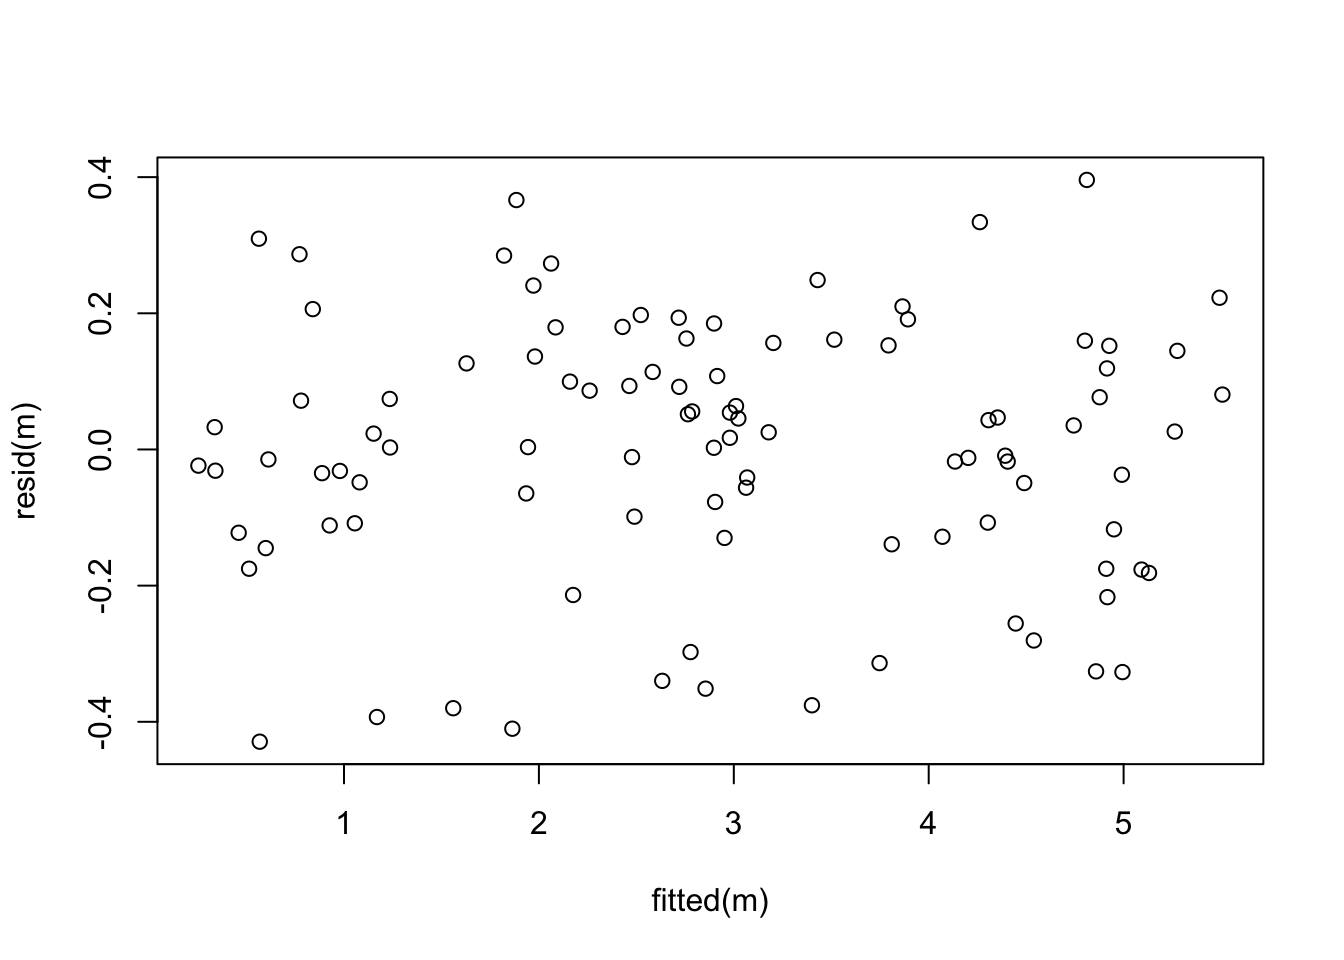
\includegraphics{MATH3714_files/figure-latex/P04Q14c-1.pdf}

Now the residual plot looks perfect!

\end{myanswers}

\textbf{16} The Prediction Error Sum of Squares (PRESS) is defined as
\begin{equation*}
  \mathrm{PRESS}
  = \sum_{i=1}^n \bigl( y_i - \hat y^{(i)}_i \bigr)^2.
\end{equation*}
Using lemma~\ref{lem:PRESS}, or otherwise, determine the PRESS
value for the \texttt{stackloss} dataset built into R (using \texttt{stack.loss}
as the response variable).

\begin{myanswers}

We can use the formula
\begin{equation*}
  \mathrm{PRESS}
  = \sum_{i=1}^n \Bigl( \frac{\hat\varepsilon_i}{1 - h_{ii}} \Bigr)^2
\end{equation*}
from the lemma. Implementation in R is straightforward.

\begin{Shaded}
\begin{Highlighting}[]
\NormalTok{m }\OtherTok{\textless{}{-}} \FunctionTok{lm}\NormalTok{(stack.loss }\SpecialCharTok{\textasciitilde{}}\NormalTok{ ., }\AttributeTok{data =}\NormalTok{ stackloss)}
\NormalTok{X }\OtherTok{\textless{}{-}} \FunctionTok{model.matrix}\NormalTok{(m)}
\NormalTok{H }\OtherTok{\textless{}{-}}\NormalTok{ X }\SpecialCharTok{\%*\%} \FunctionTok{solve}\NormalTok{(}\FunctionTok{t}\NormalTok{(X) }\SpecialCharTok{\%*\%}\NormalTok{ X, }\FunctionTok{t}\NormalTok{(X))}
\NormalTok{hii }\OtherTok{\textless{}{-}} \FunctionTok{diag}\NormalTok{(H)}
\FunctionTok{sum}\NormalTok{((}\FunctionTok{resid}\NormalTok{(m)}\SpecialCharTok{/}\NormalTok{(}\DecValTok{1} \SpecialCharTok{{-}}\NormalTok{ hii))}\SpecialCharTok{\^{}}\DecValTok{2}\NormalTok{)}
\end{Highlighting}
\end{Shaded}

\begin{Shaded}
\begin{Highlighting}[]
\NormalTok{\# [1] 291.8689}
\end{Highlighting}
\end{Shaded}

\end{myanswers}

\clearpage

\hypertarget{S14-methods}{%
\section{Methods for Model Selection}\label{S14-methods}}

For a model with \(p\) input variables, there are
\(2^p\) different choices for which variables to include in the
model (or \(2^{p+1}\), if we also have to decide whether to include the intercept).
This value increases quickly with \(p\): for \(p = 10\) we
have \(1024\) models to consider, for \(p = 20\) there are \(1048576\) possible
models, and for large \(p\) it becomes infeasible to simply try all possible
models to find the best one. In this section we consider algorithms
for finding a good selection inputs when \(p\) is large.

\hypertarget{exhaustive-search}{%
\subsection{Exhaustive Search}\label{exhaustive-search}}

Efficient algorithms are available to find the best model out of the
\(2^p\) possible models for small to moderate \(p\). Here we present
a method which can often find the model with the largest \(R^2_\mathrm{adj}\)
without having to fit all \(2^p\) models. We consider the least squares
estimate throughout.

We can characterise each possible model by the set \(J \subseteq \{1, \ldots p\}\) of variables included in the model. The model includes variable \(x_j\), if
and only if \(j \in J\). Here we assume that the intercept is always included,
so that \(J=\emptyset\) corresponds to the model \(Y = \beta_0 + \varepsilon\).

The method described in this section is based on the following three observations:

\begin{itemize}
\item
  In order to \emph{maximise} \(R^2_\mathrm{adj}\), we can equivalently also
  find the \(J\) which \emph{minimises}
  \begin{equation*}
    \hat\sigma^2(J)
      := \frac{1}{n - |J| - 1} \sum_{i=1}^n (y_i - \hat y_i)^2,
  \end{equation*}
  where \(|J|\) is the number of variables in \(J\) and the
  \(\hat y_i\) are the fitted values for the model with inputs \(j \in J\).
  We have seen that these criteria are equivalent in section~\ref{criteria}.
\item
  For \(J \subseteq \{1, \ldots p\}\), define
  \begin{equation*}
    r(J)
      := \sum_{i=1}^n (y_i - \hat y_i)^2
  \end{equation*}
  where \(\hat y_i\) are the fitted values for the model corresponding to~\(J\).
  This gives the residual sum of squares for each model. The we have
  \begin{align*}
    \min_J \hat\sigma^2(J)
      &= \min_J \frac{1}{n - |J|} \sum_{i=1}^n (y_i - \hat y_i)^2 \\
      &= \min_{q \in \{0, 1, \ldots, p\}} \min_{J, |J|=q} \frac{1}{n - q} r(J) \\
      &= \min_{q \in \{0, 1, \ldots, p\}} \frac{1}{n - q} \min_{J, |J|=q} r(J).
  \end{align*}
  This means that we can first minimise the residual sum of squares
  for each fixed number \(q\) of inputs, and then find the \(q\)
  which gives the best~\(\hat\sigma^2\) in a second step.
\item
  Adding a variables never increases the residual sum of squares.
  Thus we have \(r(J) \leq r(K)\) whenever \(J \supseteq K\).
  We can use this result to exclude certain models without having to fit them.
\end{itemize}

\hypertarget{search-algorithm}{%
\subsection{Search Algorithm}\label{search-algorithm}}

To find the model with optimal adjusted R-squared value, we perform the
following steps. The algorithm is based on the ideas explained in the previous
section.

\begin{enumerate}
\def\labelenumi{\Alph{enumi}.}
\item
  Let \(\varphi_j\) denote the residual sum of squares for the model containing
  all variables except \(x_j\):
  \begin{equation*}
        \varphi_j := r\bigl( \{ 1, \ldots, p \} \setminus \{ j \} \bigr).
    \end{equation*}
  Suppose that the \(x_j\) are ordered so that
  \begin{equation*}
        \varphi_1 \geq \varphi_2 \geq \cdots \geq \varphi_p.
    \end{equation*}
  Any model \(J\) with \(j \notin J\) has \(r(J) \geq \varphi_j\).
\item
  Compute \(\min_{J, |J|=0} r(J) = r(\emptyset)\). This is the residual
  sum of squares of the model which consists only of the intercept.
\item
  For each \(q := 1, \ldots, p-2\):

  \begin{enumerate}
  \def\labelenumii{\arabic{enumii}.}
  \item
    Let
    \begin{equation*}
         r := r\bigl( \{1, \ldots, q\} \bigr).
     \end{equation*}
    This is the only model with \(q\) inputs where the first
    excluded variable has index \(k = q+1\).
    If \(r \leq \varphi_{k-1} = \varphi_q\), we know from step~A that
    \(J = \{1, \ldots, q\}\) is the best
    model with \(q\) inputs, since any other model will exclude
    one of the \(x_j\) with \(j \leq q\).
    In this case we have found
    \begin{equation*}
       \min_{J, |J|=q} r(J)
       = r.
     \end{equation*}
    and we continue step B by trying the next value of~\(q\).
    If \(r > \varphi_{k-1}\), no decision can be taken at this point and we
    continue with step~2.
  \item
    For \(j \in \{q+1, \ldots, p\}\) let
    \begin{equation*}
         r_j := r\bigl( \{1, \ldots, q-1\} \cup \{j\} \bigr).
     \end{equation*}
    These are all models with \(q\) inputs where the first excluded
    variable has index \(k = q\).
    If \(\min(r, r_1, \ldots, r_q) \leq \varphi_{k-1} = \varphi_{q-1}\), then we know
    from step~A that the \(J\) corresponing to the minimum is the best model
    with \(q\) inputs. In this case we continue step B by trying the next
    value of~\(q\). Otherwise we proceed to step~3.
  \item
    Similarly to the previous step, we consider all models with \(q\)
    variables where the first excluded variable has index \(k = q-1\).
    If the best RSS amonst these and the previously considered
    models is less than or equal to \(\varphi_{k-1}\) we are done
    and consider the next \(q\). Otherwise we decrease \(k\) until we reach
    \(k = 1\). At this point we have considered all models with \(q\)
    variables and have found \(\min_{J, |J|=q} r(J)\).
  \end{enumerate}
\item
  Compute \(\min_{J, |J|=p-1} r(J) = \min_{j \in \{1, \ldots, p\}} \varphi_j\).
\item
  Compute \(\min_{J, |J|=p} r(J) = r\bigl( \{1, \ldots, p\} \bigr)\).
\item
  Find the \(q \in \{0, \ldots, p\}\) for which \(\min_{J, |J|=q} r(J) / (n-q-1)\)
  is smallest. Output the model which has minimal RSS for this~\(q\).
\end{enumerate}

This algorithm finds the model with the maximal \(R^2_\mathrm{adj}\).
Often, large savings are achieved by the early exits in step~C.
Only in the worst case, when all of the comparisons with \(\varphi_j\) in step
C fail, this algorithms needs to fit all \(2^p\) models.

\begin{example}
\protect\hypertarget{exm:qsar-search}{}\label{exm:qsar-search}To demonstrate the steps of the algorithm, we implement the method
``by hand''. We use the QSAR dataset, which we have already seen
in section~\ref{S07-examples}:

\begin{Shaded}
\begin{Highlighting}[]
\CommentTok{\# data from https://archive.ics.uci.edu/ml/datasets/QSAR+aquatic+toxicity}
\NormalTok{qsar }\OtherTok{\textless{}{-}} \FunctionTok{read.csv}\NormalTok{(}\StringTok{"data/qsar\_aquatic\_toxicity.csv"}\NormalTok{,}
                 \AttributeTok{sep =} \StringTok{";"}\NormalTok{, }\AttributeTok{header =} \ConstantTok{FALSE}\NormalTok{)}
\NormalTok{fields }\OtherTok{\textless{}{-}} \FunctionTok{c}\NormalTok{(}
    \StringTok{"TPSA"}\NormalTok{,}
    \StringTok{"SAacc"}\NormalTok{,}
    \StringTok{"H050"}\NormalTok{,}
    \StringTok{"MLOGP"}\NormalTok{,}
    \StringTok{"RDCHI"}\NormalTok{,}
    \StringTok{"GATS1p"}\NormalTok{,}
    \StringTok{"nN"}\NormalTok{,}
    \StringTok{"C040"}\NormalTok{,}
    \StringTok{"LC50"}
\NormalTok{)}
\FunctionTok{names}\NormalTok{(qsar) }\OtherTok{\textless{}{-}}\NormalTok{ fields}
\end{Highlighting}
\end{Shaded}

To make it easy to add/remove columns automatically, we first construct
the design matrix, remove columns as needed, and then use the resulting
matrix in the call to \texttt{lm()} (instead of specifying the terms to include
by name).

\begin{Shaded}
\begin{Highlighting}[]
\NormalTok{X }\OtherTok{\textless{}{-}} \FunctionTok{model.matrix}\NormalTok{(LC50 }\SpecialCharTok{\textasciitilde{}}\NormalTok{ ., }\AttributeTok{data =}\NormalTok{ qsar)}
\NormalTok{X }\OtherTok{\textless{}{-}}\NormalTok{ X[, }\SpecialCharTok{{-}}\DecValTok{1}\NormalTok{] }\CommentTok{\# remove the intercept, since lm() will re{-}add it later}
\NormalTok{n }\OtherTok{\textless{}{-}} \FunctionTok{nrow}\NormalTok{(X)}
\NormalTok{p }\OtherTok{\textless{}{-}} \FunctionTok{ncol}\NormalTok{(X)}

\NormalTok{y }\OtherTok{\textless{}{-}}\NormalTok{ qsar}\SpecialCharTok{$}\NormalTok{LC50}

\NormalTok{m }\OtherTok{\textless{}{-}} \FunctionTok{lm}\NormalTok{(y }\SpecialCharTok{\textasciitilde{}}\NormalTok{ X) }\CommentTok{\# full model}
\FunctionTok{summary}\NormalTok{(m)}
\end{Highlighting}
\end{Shaded}

\begin{Shaded}
\begin{Highlighting}[]
\NormalTok{\# }
\NormalTok{\# Call:}
\NormalTok{\# lm(formula = y \textasciitilde{} X)}
\NormalTok{\# }
\NormalTok{\# Residuals:}
\NormalTok{\#     Min      1Q  Median      3Q     Max }
\NormalTok{\# {-}4.4934 {-}0.7579 {-}0.1120  0.5829  4.9778 }
\NormalTok{\# }
\NormalTok{\# Coefficients:}
\NormalTok{\#              Estimate Std. Error t value Pr(\textgreater{}|t|)    }
\NormalTok{\# (Intercept)  2.698887   0.244554  11.036  \textless{} 2e{-}16 ***}
\NormalTok{\# XTPSA        0.027201   0.002661  10.220  \textless{} 2e{-}16 ***}
\NormalTok{\# XSAacc      {-}0.015081   0.002091  {-}7.211 1.90e{-}12 ***}
\NormalTok{\# XH050        0.040619   0.059787   0.679 0.497186    }
\NormalTok{\# XMLOGP       0.446108   0.063296   7.048 5.60e{-}12 ***}
\NormalTok{\# XRDCHI       0.513928   0.135565   3.791 0.000167 ***}
\NormalTok{\# XGATS1p     {-}0.571313   0.153882  {-}3.713 0.000227 ***}
\NormalTok{\# XnN         {-}0.224751   0.048301  {-}4.653 4.12e{-}06 ***}
\NormalTok{\# XC040        0.003194   0.077972   0.041 0.967340    }
\NormalTok{\# {-}{-}{-}}
\NormalTok{\# Signif. codes:  0 \textquotesingle{}***\textquotesingle{} 0.001 \textquotesingle{}**\textquotesingle{} 0.01 \textquotesingle{}*\textquotesingle{} 0.05 \textquotesingle{}.\textquotesingle{} 0.1 \textquotesingle{} \textquotesingle{} 1}
\NormalTok{\# }
\NormalTok{\# Residual standard error: 1.203 on 537 degrees of freedom}
\NormalTok{\# Multiple R{-}squared:  0.4861,  Adjusted R{-}squared:  0.4785 }
\NormalTok{\# F{-}statistic:  63.5 on 8 and 537 DF,  p{-}value: \textless{} 2.2e{-}16}
\end{Highlighting}
\end{Shaded}

Comparing the output to what we have seen in section~\ref{S07-examples}
shows that the new method of calling \texttt{lm()} gives the same results
as before. Now we follow the steps of the algorithm.

\textbf{A.} The values \(\varphi_1, \ldots, \varphi_p\) can be computed as follows:

\begin{Shaded}
\begin{Highlighting}[]
\NormalTok{phi }\OtherTok{\textless{}{-}} \FunctionTok{numeric}\NormalTok{(p) }\CommentTok{\# pre{-}allocate an empty vector}
\ControlFlowTok{for}\NormalTok{ (j }\ControlFlowTok{in} \DecValTok{1}\SpecialCharTok{:}\NormalTok{p) \{}
\NormalTok{    idx }\OtherTok{\textless{}{-}}\NormalTok{ (}\DecValTok{1}\SpecialCharTok{:}\NormalTok{p)[}\SpecialCharTok{{-}}\NormalTok{j] }\CommentTok{\# all variables except x[j]}
\NormalTok{    m }\OtherTok{\textless{}{-}} \FunctionTok{lm}\NormalTok{(y }\SpecialCharTok{\textasciitilde{}}\NormalTok{ X[,idx])}
\NormalTok{    phi[j] }\OtherTok{\textless{}{-}} \FunctionTok{sum}\NormalTok{(}\FunctionTok{resid}\NormalTok{(m)}\SpecialCharTok{\^{}}\DecValTok{2}\NormalTok{)}
\NormalTok{\}}

\CommentTok{\# change the order of columns in X, so that the phi\_j are decreasing}
\NormalTok{jj }\OtherTok{\textless{}{-}} \FunctionTok{order}\NormalTok{(phi, }\AttributeTok{decreasing =} \ConstantTok{TRUE}\NormalTok{)}
\NormalTok{X }\OtherTok{\textless{}{-}}\NormalTok{ X[, jj]}
\NormalTok{phi }\OtherTok{\textless{}{-}}\NormalTok{ phi[jj]}
\FunctionTok{plot}\NormalTok{(phi, }\AttributeTok{xlab =} \StringTok{"j"}\NormalTok{, }\AttributeTok{ylab =} \FunctionTok{expression}\NormalTok{(varphi[j]))}
\end{Highlighting}
\end{Shaded}

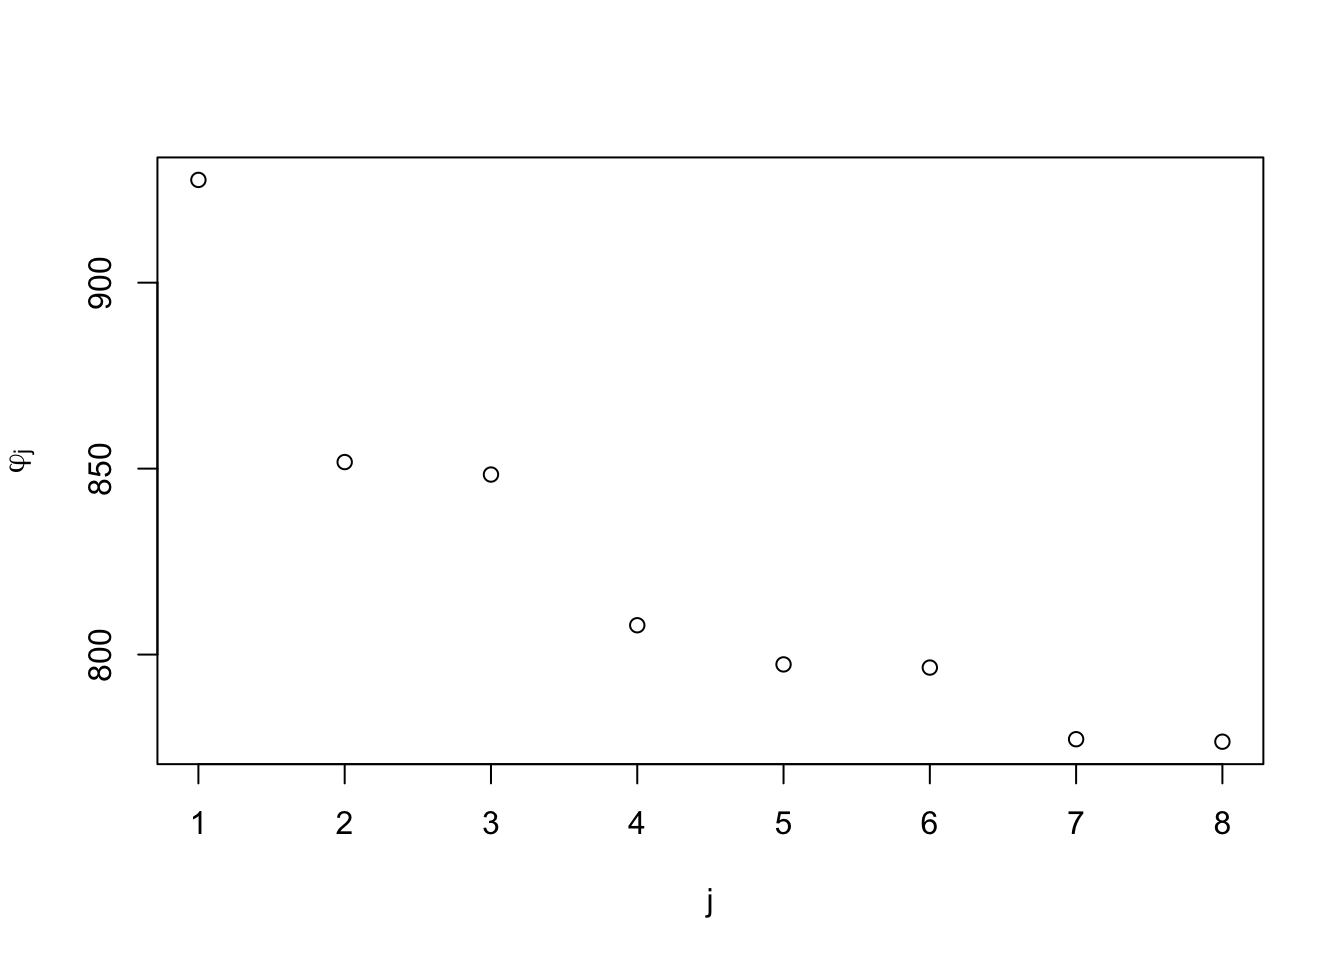
\includegraphics{MATH3714_files/figure-latex/exhaustiveA-1.pdf}

The plot shows the residual sum of squares for the model with input \(x_j\)
omitted, for \(j\) ranging from 1 to~8.

\textbf{B.} Next, we compute the residual
sum of squares of the model which consists only of the intercept.
This is the case \(q = 0\).

\begin{Shaded}
\begin{Highlighting}[]
\NormalTok{all.q }\OtherTok{\textless{}{-}} \DecValTok{0}\SpecialCharTok{:}\NormalTok{p}
\NormalTok{best.rss }\OtherTok{\textless{}{-}} \FunctionTok{numeric}\NormalTok{(p }\SpecialCharTok{+} \DecValTok{1}\NormalTok{) }\CommentTok{\# For storing the best RSS for q = 0, ..., p,}
\NormalTok{best.model }\OtherTok{\textless{}{-}} \FunctionTok{vector}\NormalTok{(}\StringTok{"list"}\NormalTok{, p }\SpecialCharTok{+} \DecValTok{1}\NormalTok{) }\CommentTok{\# and the corresponding models.}

\NormalTok{m }\OtherTok{\textless{}{-}} \FunctionTok{lm}\NormalTok{(y }\SpecialCharTok{\textasciitilde{}} \DecValTok{1}\NormalTok{)}
\NormalTok{best.rss[}\DecValTok{0} \SpecialCharTok{+} \DecValTok{1}\NormalTok{] }\OtherTok{\textless{}{-}} \FunctionTok{sum}\NormalTok{(}\FunctionTok{resid}\NormalTok{(m)}\SpecialCharTok{\^{}}\DecValTok{2}\NormalTok{)}
\NormalTok{best.model[[}\DecValTok{0} \SpecialCharTok{+} \DecValTok{1}\NormalTok{]] }\OtherTok{\textless{}{-}} \FunctionTok{integer}\NormalTok{(}\DecValTok{0}\NormalTok{) }\CommentTok{\# a vector of length 0 (no columns)}

\NormalTok{count }\OtherTok{\textless{}{-}} \DecValTok{1} \CommentTok{\# number of models fitted so far}
\end{Highlighting}
\end{Shaded}

\textbf{C.} Now we consider \(q \in \{1, \ldots, p-2\}\). The algorithm groups
these cases by the position \(k\) of the first column omitted in the model,
starting with \(k = q+1\) and then decreasing \(k\) in each step.
We use the function \texttt{combn} from the \texttt{sets} package
to get all possible choices of
\(q - k + 1\) columns out of \(\{k+1, \ldots, p\}\).

\begin{Shaded}
\begin{Highlighting}[]
\FunctionTok{library}\NormalTok{(sets) }\CommentTok{\# this defines "combn()"}
\ControlFlowTok{for}\NormalTok{ (q }\ControlFlowTok{in} \DecValTok{1}\SpecialCharTok{:}\NormalTok{(p}\DecValTok{{-}2}\NormalTok{)) \{}
\NormalTok{    best.rss[q }\SpecialCharTok{+} \DecValTok{1}\NormalTok{] }\OtherTok{\textless{}{-}} \ConstantTok{Inf}

    \CommentTok{\# Consider all sets of q columns, ...}
    \ControlFlowTok{for}\NormalTok{ (k }\ControlFlowTok{in}\NormalTok{ (q}\SpecialCharTok{+}\DecValTok{1}\NormalTok{)}\SpecialCharTok{:}\DecValTok{1}\NormalTok{) \{}
        \CommentTok{\# ... where the first omitted column is k.}

        \CommentTok{\# We have to include 1, ..., k{-}1, and ...}
\NormalTok{        a }\OtherTok{\textless{}{-}} \FunctionTok{seq\_len}\NormalTok{(k}\DecValTok{{-}1}\NormalTok{)}

        \CommentTok{\# ... for the remaining q {-} (k{-}1) inputs, we try all}
        \CommentTok{\# possible combinations.}
\NormalTok{        bb }\OtherTok{\textless{}{-}} \FunctionTok{combn}\NormalTok{((k}\SpecialCharTok{+}\DecValTok{1}\NormalTok{)}\SpecialCharTok{:}\NormalTok{p, q }\SpecialCharTok{{-}}\NormalTok{ k }\SpecialCharTok{+} \DecValTok{1}\NormalTok{)}
        \ControlFlowTok{for}\NormalTok{ (l }\ControlFlowTok{in} \FunctionTok{seq\_len}\NormalTok{(}\FunctionTok{ncol}\NormalTok{(bb))) \{}
\NormalTok{            b }\OtherTok{\textless{}{-}}\NormalTok{ bb[, l]}
\NormalTok{            included }\OtherTok{\textless{}{-}} \FunctionTok{c}\NormalTok{(a, b)}

\NormalTok{            m }\OtherTok{\textless{}{-}} \FunctionTok{lm}\NormalTok{(y }\SpecialCharTok{\textasciitilde{}}\NormalTok{ X[, included])}
\NormalTok{            count }\OtherTok{\textless{}{-}}\NormalTok{ count }\SpecialCharTok{+} \DecValTok{1}
\NormalTok{            rss }\OtherTok{\textless{}{-}} \FunctionTok{sum}\NormalTok{(}\FunctionTok{resid}\NormalTok{(m)}\SpecialCharTok{\^{}}\DecValTok{2}\NormalTok{)}

            \ControlFlowTok{if}\NormalTok{ (rss }\SpecialCharTok{\textless{}}\NormalTok{ best.rss[q }\SpecialCharTok{+} \DecValTok{1}\NormalTok{]) \{}
\NormalTok{                best.rss[q }\SpecialCharTok{+} \DecValTok{1}\NormalTok{] }\OtherTok{\textless{}{-}}\NormalTok{ rss}
\NormalTok{                best.model[[q }\SpecialCharTok{+} \DecValTok{1}\NormalTok{]] }\OtherTok{\textless{}{-}}\NormalTok{ included}
\NormalTok{            \}}
\NormalTok{        \}}

        \ControlFlowTok{if}\NormalTok{ (k }\SpecialCharTok{\textgreater{}} \DecValTok{1} \SpecialCharTok{\&\&}\NormalTok{ best.rss[q] }\SpecialCharTok{\textless{}=}\NormalTok{ phi[k}\DecValTok{{-}1}\NormalTok{]) \{}
            \CommentTok{\# If we reach this point, we know that we found the best}
            \CommentTok{\# arrangement and we can exit the loop over k early.}
            \CommentTok{\# This is what makes the algorithm efficient.}
            \ControlFlowTok{break}
\NormalTok{        \}}
\NormalTok{    \}}
\NormalTok{\}}
\end{Highlighting}
\end{Shaded}

\textbf{D.} We already fitted all models with \(p-1\) inputs, when we computed~\texttt{phi}.
Since we sorted the models, the best of these models is last in the list.
This covers the case \(q = p - 1\).

\begin{Shaded}
\begin{Highlighting}[]
\NormalTok{best.rss[(p }\SpecialCharTok{{-}} \DecValTok{1}\NormalTok{) }\SpecialCharTok{+} \DecValTok{1}\NormalTok{] }\OtherTok{\textless{}{-}} \FunctionTok{min}\NormalTok{(phi)}
\NormalTok{omitted }\OtherTok{\textless{}{-}}\NormalTok{ jj[}\FunctionTok{length}\NormalTok{(jj)]}
\NormalTok{best.model[[(p }\SpecialCharTok{{-}} \DecValTok{1}\NormalTok{) }\SpecialCharTok{+} \DecValTok{1}\NormalTok{]] }\OtherTok{\textless{}{-}}\NormalTok{ (}\DecValTok{1}\SpecialCharTok{:}\NormalTok{p)[}\SpecialCharTok{{-}}\NormalTok{omitted]}
\NormalTok{count }\OtherTok{\textless{}{-}}\NormalTok{ count }\SpecialCharTok{+} \FunctionTok{length}\NormalTok{(phi)}
\end{Highlighting}
\end{Shaded}

\textbf{E.} Finally, for \(q = p\) we fit the full model:

\begin{Shaded}
\begin{Highlighting}[]
\NormalTok{m }\OtherTok{\textless{}{-}} \FunctionTok{lm}\NormalTok{(y }\SpecialCharTok{\textasciitilde{}}\NormalTok{ X)}
\NormalTok{best.rss[p }\SpecialCharTok{+} \DecValTok{1}\NormalTok{] }\OtherTok{\textless{}{-}} \FunctionTok{sum}\NormalTok{(}\FunctionTok{resid}\NormalTok{(m)}\SpecialCharTok{\^{}}\DecValTok{2}\NormalTok{)}
\NormalTok{best.model[[p }\SpecialCharTok{+} \DecValTok{1}\NormalTok{]] }\OtherTok{\textless{}{-}} \DecValTok{1}\SpecialCharTok{:}\NormalTok{p}
\NormalTok{count }\OtherTok{\textless{}{-}}\NormalTok{ count }\SpecialCharTok{+} \DecValTok{1}
\end{Highlighting}
\end{Shaded}

\textbf{F.} Now we can find the model with the best \(R^2_\mathrm{adj}\):

\begin{Shaded}
\begin{Highlighting}[]
\FunctionTok{plot}\NormalTok{(all.q, best.rss }\SpecialCharTok{/}\NormalTok{ (n }\SpecialCharTok{{-}}\NormalTok{ all.q }\SpecialCharTok{{-}} \DecValTok{1}\NormalTok{),}
     \AttributeTok{xlab =} \StringTok{"q"}\NormalTok{, }\AttributeTok{ylab =} \StringTok{"residual variance"}\NormalTok{)}
\NormalTok{best.q }\OtherTok{\textless{}{-}} \FunctionTok{which.min}\NormalTok{(best.rss }\SpecialCharTok{/}\NormalTok{ (n }\SpecialCharTok{{-}}\NormalTok{ all.q }\SpecialCharTok{{-}}\NormalTok{ q))}
\FunctionTok{abline}\NormalTok{(}\AttributeTok{v =}\NormalTok{ best.q)}
\end{Highlighting}
\end{Shaded}

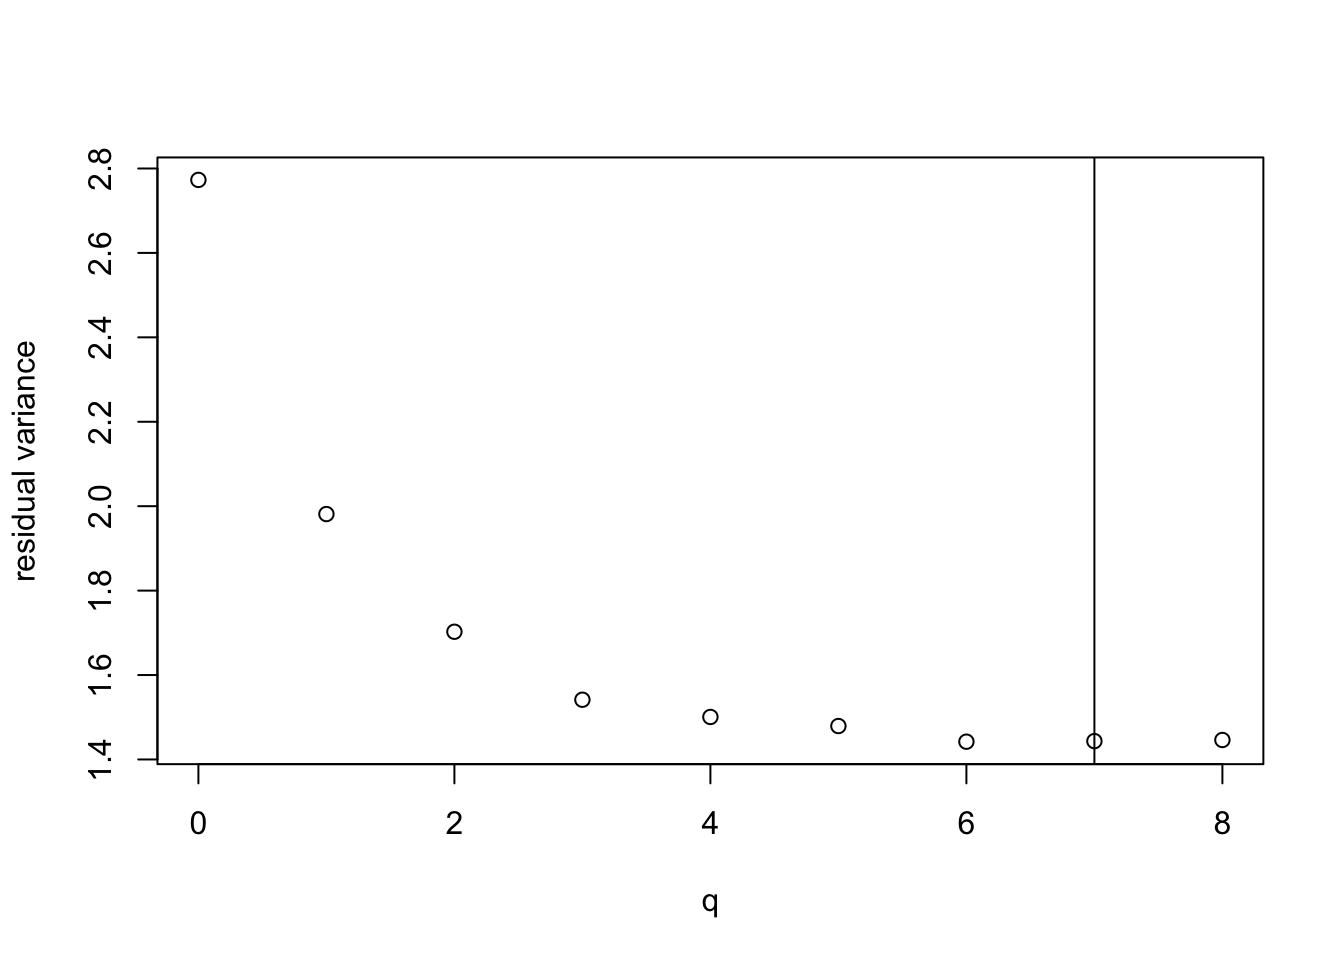
\includegraphics{MATH3714_files/figure-latex/exhaustiveB-1.pdf}

We see that the model with \(q = 7\) variables has the the
lowest \(\hat\sigma^2\) and thus the highest \(R^2_\mathrm{adj}\).
The values for \(q = 6\) and \(q = 8\) are very close to
optimal. The best model uses the following variables:

\begin{Shaded}
\begin{Highlighting}[]
\FunctionTok{colnames}\NormalTok{(X)[best.model[[}\DecValTok{7} \SpecialCharTok{+} \DecValTok{1}\NormalTok{]]]}
\end{Highlighting}
\end{Shaded}

\begin{Shaded}
\begin{Highlighting}[]
\NormalTok{\# [1] "TPSA"   "SAacc"  "MLOGP"  "nN"     "RDCHI"  "GATS1p" "H050"}
\end{Highlighting}
\end{Shaded}

We can fit the optimal model from the original data:

\begin{Shaded}
\begin{Highlighting}[]
\NormalTok{m.best }\OtherTok{\textless{}{-}} \FunctionTok{lm}\NormalTok{(LC50 }\SpecialCharTok{\textasciitilde{}}\NormalTok{ TPSA }\SpecialCharTok{+}\NormalTok{ SAacc }\SpecialCharTok{+}\NormalTok{ MLOGP }\SpecialCharTok{+}\NormalTok{ nN }\SpecialCharTok{+}\NormalTok{ RDCHI }\SpecialCharTok{+}\NormalTok{ GATS1p }\SpecialCharTok{+}\NormalTok{ H050,}
             \AttributeTok{data =}\NormalTok{ qsar)}
\FunctionTok{summary}\NormalTok{(m.best)}
\end{Highlighting}
\end{Shaded}

\begin{Shaded}
\begin{Highlighting}[]
\NormalTok{\# }
\NormalTok{\# Call:}
\NormalTok{\# lm(formula = LC50 \textasciitilde{} TPSA + SAacc + MLOGP + nN + RDCHI + GATS1p + }
\NormalTok{\#     H050, data = qsar)}
\NormalTok{\# }
\NormalTok{\# Residuals:}
\NormalTok{\#     Min      1Q  Median      3Q     Max }
\NormalTok{\# {-}4.4951 {-}0.7585 {-}0.1125  0.5838  4.9769 }
\NormalTok{\# }
\NormalTok{\# Coefficients:}
\NormalTok{\#              Estimate Std. Error t value Pr(\textgreater{}|t|)    }
\NormalTok{\# (Intercept)  2.698271   0.243863  11.065  \textless{} 2e{-}16 ***}
\NormalTok{\# TPSA         0.027193   0.002651  10.256  \textless{} 2e{-}16 ***}
\NormalTok{\# SAacc       {-}0.015056   0.002001  {-}7.523 2.26e{-}13 ***}
\NormalTok{\# MLOGP        0.445763   0.062674   7.112 3.65e{-}12 ***}
\NormalTok{\# nN          {-}0.224511   0.047900  {-}4.687 3.52e{-}06 ***}
\NormalTok{\# RDCHI        0.514866   0.133492   3.857 0.000129 ***}
\NormalTok{\# GATS1p      {-}0.571629   0.153546  {-}3.723 0.000218 ***}
\NormalTok{\# H050         0.039811   0.056388   0.706 0.480485    }
\NormalTok{\# {-}{-}{-}}
\NormalTok{\# Signif. codes:  0 \textquotesingle{}***\textquotesingle{} 0.001 \textquotesingle{}**\textquotesingle{} 0.01 \textquotesingle{}*\textquotesingle{} 0.05 \textquotesingle{}.\textquotesingle{} 0.1 \textquotesingle{} \textquotesingle{} 1}
\NormalTok{\# }
\NormalTok{\# Residual standard error: 1.201 on 538 degrees of freedom}
\NormalTok{\# Multiple R{-}squared:  0.4861,  Adjusted R{-}squared:  0.4795 }
\NormalTok{\# F{-}statistic: 72.71 on 7 and 538 DF,  p{-}value: \textless{} 2.2e{-}16}
\end{Highlighting}
\end{Shaded}

This shows that \(R^2_\mathrm{adj}\) has indeed marginally inproved,
from \(0.4785\) to \(0.4795\)

To conclude, we check that the complicated algorithm indeed saved some work:

\begin{Shaded}
\begin{Highlighting}[]
\NormalTok{total }\OtherTok{\textless{}{-}} \DecValTok{2}\SpecialCharTok{\^{}}\NormalTok{p}
\FunctionTok{cat}\NormalTok{(count,}
    \StringTok{" models fitted ("}\NormalTok{, }\FunctionTok{round}\NormalTok{(}\DecValTok{100} \SpecialCharTok{*}\NormalTok{ count }\SpecialCharTok{/}\NormalTok{ total,}\DecValTok{1}\NormalTok{ ), }\StringTok{"\%)}\SpecialCharTok{\textbackslash{}n}\StringTok{"}\NormalTok{,}
    \AttributeTok{sep =} \StringTok{""}\NormalTok{)}
\end{Highlighting}
\end{Shaded}

\begin{Shaded}
\begin{Highlighting}[]
\NormalTok{\# 88 models fitted (34.4\%)}
\end{Highlighting}
\end{Shaded}

This shows that we only needed to fit 88 of the 256 models under consideration.
\end{example}

\begin{example}
We can perform the analysis from the previous example automatically,
using the function \texttt{regsubsets()} from the \texttt{leaps} package:

\begin{Shaded}
\begin{Highlighting}[]
\FunctionTok{library}\NormalTok{(leaps)}
\NormalTok{m }\OtherTok{\textless{}{-}} \FunctionTok{regsubsets}\NormalTok{(LC50 }\SpecialCharTok{\textasciitilde{}}\NormalTok{ ., }\AttributeTok{data =}\NormalTok{ qsar,}
                \AttributeTok{method =} \StringTok{"exhaustive"}\NormalTok{)}
\FunctionTok{summary}\NormalTok{(m)}
\end{Highlighting}
\end{Shaded}

\begin{Shaded}
\begin{Highlighting}[]
\NormalTok{\# Subset selection object}
\NormalTok{\# Call: regsubsets.formula(LC50 \textasciitilde{} ., data = qsar, method = "exhaustive")}
\NormalTok{\# 8 Variables  (and intercept)}
\NormalTok{\#        Forced in Forced out}
\NormalTok{\# TPSA       FALSE      FALSE}
\NormalTok{\# SAacc      FALSE      FALSE}
\NormalTok{\# H050       FALSE      FALSE}
\NormalTok{\# MLOGP      FALSE      FALSE}
\NormalTok{\# RDCHI      FALSE      FALSE}
\NormalTok{\# GATS1p     FALSE      FALSE}
\NormalTok{\# nN         FALSE      FALSE}
\NormalTok{\# C040       FALSE      FALSE}
\NormalTok{\# 1 subsets of each size up to 8}
\NormalTok{\# Selection Algorithm: exhaustive}
\NormalTok{\#          TPSA SAacc H050 MLOGP RDCHI GATS1p nN  C040}
\NormalTok{\# 1  ( 1 ) " "  " "   " "  "*"   " "   " "    " " " " }
\NormalTok{\# 2  ( 1 ) "*"  " "   " "  "*"   " "   " "    " " " " }
\NormalTok{\# 3  ( 1 ) "*"  "*"   " "  "*"   " "   " "    " " " " }
\NormalTok{\# 4  ( 1 ) "*"  "*"   " "  "*"   " "   " "    "*" " " }
\NormalTok{\# 5  ( 1 ) "*"  "*"   " "  "*"   " "   "*"    "*" " " }
\NormalTok{\# 6  ( 1 ) "*"  "*"   " "  "*"   "*"   "*"    "*" " " }
\NormalTok{\# 7  ( 1 ) "*"  "*"   "*"  "*"   "*"   "*"    "*" " " }
\NormalTok{\# 8  ( 1 ) "*"  "*"   "*"  "*"   "*"   "*"    "*" "*"}
\end{Highlighting}
\end{Shaded}

This shows the best model of each size. The only step left is
to decide which \(q\) to use. This choice depends on the cost-complexity
tradeoff. Here we consider \(R^2_\mathrm{adj}\) again:

\begin{Shaded}
\begin{Highlighting}[]
\FunctionTok{round}\NormalTok{(}\FunctionTok{summary}\NormalTok{(m)}\SpecialCharTok{$}\NormalTok{adjr2, }\DecValTok{4}\NormalTok{)}
\end{Highlighting}
\end{Shaded}

\begin{Shaded}
\begin{Highlighting}[]
\NormalTok{\# [1] 0.2855 0.3860 0.4441 0.4588 0.4666 0.4799 0.4795 0.4785}
\end{Highlighting}
\end{Shaded}

This gives the \(R^2_\mathrm{adj}\) for the optimal model of each size
again. At the end of the list we recognise the values \texttt{0.4795} and
\texttt{0.4785} from our previous analysis.
\end{example}

\hypertarget{other-methods}{%
\subsection{Other Methods}\label{other-methods}}

There are other, approximate methods available which can be used
when the number \(p\) of model parameters is too large for an exhaustives
search.

\hypertarget{stepwise-forward-selection}{%
\subsubsection{Stepwise Forward Selection}\label{stepwise-forward-selection}}

Here the idea is to start with a minimal model, and then add variables one by
one, until no further (large enough) improvements can be achieved.

Start with only intercept term: \(y=\beta_0 + \varepsilon\), then
consider each of \(p\) models:
\begin{equation*}
  y
  = \beta_0 + \beta_j x_j + \varepsilon,
\end{equation*}
for \(j \in \{1, \ldots, p\}\).

Choose the model with the smallest residual sum of squares, provided that the
``significance of the fitted model'' achieves a specified threshold. The process
continues by adding more variables, one at a time, until either

\begin{itemize}
\tightlist
\item
  All variables are in the model.
\item
  The significance level can not be achieved by any variable not in the model.
\end{itemize}

The ``significance of the model'' can be examined by considering a
\(t\)-test as in lemma~\ref{lem:t-test}.

\hypertarget{stepwise-backward-selection}{%
\subsubsection{Stepwise Backward Selection}\label{stepwise-backward-selection}}

Here the idea is to start with the full model, and to remove variables
one by one until no good enough candidates for removal are left.

In each step we consider the test statistic \(|T_j|\) for the tests
\begin{equation*}
  H_0\colon \beta_j = 0
  \quad\mbox{\textit{vs.}}\quad
  H_1\colon \beta_j \neq 0
\end{equation*}
for \(j \in \{1, \ldots, p\}\), again as in lemma~\ref{lem:t-test}.
The method selects \(x_j\) corresponding to the smallest \(|T_j|\).
If this is below a given threshold, then remove \(x_j\) and re-fit the model.
Repeat until either:

\begin{itemize}
\tightlist
\item
  No variables are left in the model.
\item
  The smallest \(|T_j|\) is above the threshold.
\end{itemize}

\hypertarget{hybrid-methods}{%
\subsubsection{Hybrid Methods}\label{hybrid-methods}}

Either start with a full model or just intercept. At each stage consider:

\begin{itemize}
\tightlist
\item
  removing least significant variable already in the model,
\item
  adding most significant variable not currently in the model,
\end{itemize}

with significance levels set to avoid a cyclical behaviour.

\textbf{Summary}

\begin{itemize}
\tightlist
\item
  We discussed different algorithms to perform model selection in practice.
\end{itemize}

\clearpage

\hypertarget{S15-factors}{%
\section{Factors}\label{S15-factors}}

In this section we will learn how to fit linear models when some or all
of the inputs are categorical. Such inputs are sometimes called ``factors''.
These can be
binary (\emph{e.g.}~sex recorded as male/female)
or ordered (\emph{e.g.}~quality recorded as poor/medium/good)
or unordered (\emph{e.g.}~marital status recorded as single/married/divorced/widowed).

\hypertarget{indicator-variables}{%
\subsection{Indicator Variables}\label{indicator-variables}}

Our aim here is to include categorical input variables within the
usual regression model
\begin{equation*}
  y
  = X\beta + \varepsilon.
\end{equation*}

Assume that \(x_j \in \{a_1, \ldots, a_k\}\) is a factor which has \(k\) possible
values. The possible values of the factor, \(a_1, \ldots, a_k\) are also called
the \textbf{levels} of the factor. The easiest way to include a factor in a
regression model is via \textbf{indicator variables}. For this we represent \(x_j\)
using \(k-1\) columns in the design matrix, say \(\tilde x_1, \ldots, \tilde x_{k-1}\), where
\begin{equation*}
  \tilde x_{\ell i}
  = \begin{cases}
    1 & \mbox{if $x_{ji} = a_\ell$ and} \\
    0 & \mbox{otherwise,}
  \end{cases}
\end{equation*}
for all \(\ell \in \{1, \ldots, k-1\}\) and \(i \in \{1, \ldots, n\}\).
Using this convention, \(x_{ji} = k\) is represented by setting
\(\tilde x_{1,i} = \cdots = \tilde x_{k-1,i} = 0\). The value \(a_k\)
which is not represented as a separate column is called the
\textbf{reference level}. The regression coefficients corresponding to the
columns \(\tilde x_1, \ldots, \tilde x_{k-1}\) can be interpreted
as the effect of level \(a_\ell\), relative to the effect
of level \(a_k\). Since the indicator is constant \(1\) for all samples
corresponding to a given factor, regression coefficients representing factors
lead to changes of the intercept, rather than of slopes.

We are using only \(k-1\) columns to represent a factor
with \(k\) levels in order to avoid collinearity. If we would use \(k\) columns,
defined as above, we would get
\begin{equation*}
  \sum_{\ell=1}^k \tilde x_{\ell i}
  = \mathbf{1},
\end{equation*}
and in a model with an intercept we would have exact collinearity of
the corresponding columns in the design matrix~\(X\).

\begin{example}

Consider a dataset consisting of a numerical input variable
and a binary factor for gender (\texttt{female}, \texttt{male}).
Assume we are given data
\((1, \mathrm{male})\), \((2, \mathrm{female})\), \((3, \mathrm{female})\).
Then we can encode this data using the following design matrix:

\begin{longtable}[]{@{}ccc@{}}
\toprule
intercept & \(x_1\) & \(1_\mathrm{\{female\}}(x_2)\) \\
\midrule
\endhead
1 & 1 & 0 \\
1 & 2 & 1 \\
1 & 3 & 1 \\
\bottomrule
\end{longtable}

\end{example}

In R there is a dedicated type \texttt{factor} for categorical variables.
If factors appear in the input of linear regression problem, the
function \texttt{lm()} will automatically create the indicator variables
for us.

\begin{example}
Here we simulated data which could describe the effect of some
medical treatment.
In the simulated data we have two groups, one which has been ``treated''
and a control group. There is a ``value'' which decreases with age,
and is lower for the group which has been treated (the intercept is 10
instead of 12).

\begin{Shaded}
\begin{Highlighting}[]
\NormalTok{age1 }\OtherTok{\textless{}{-}} \FunctionTok{runif}\NormalTok{(}\DecValTok{25}\NormalTok{, }\DecValTok{18}\NormalTok{, }\DecValTok{40}\NormalTok{)}
\NormalTok{group1 }\OtherTok{\textless{}{-}} \FunctionTok{data.frame}\NormalTok{(}
    \AttributeTok{value=}\DecValTok{10} \SpecialCharTok{{-}} \FloatTok{0.2} \SpecialCharTok{*}\NormalTok{ age1 }\SpecialCharTok{+} \FunctionTok{rnorm}\NormalTok{(}\DecValTok{25}\NormalTok{, }\AttributeTok{sd=}\FloatTok{0.5}\NormalTok{),}
    \AttributeTok{age=}\NormalTok{age1,}
    \AttributeTok{treated=}\StringTok{"yes"}\NormalTok{)}
\NormalTok{age2 }\OtherTok{\textless{}{-}} \FunctionTok{runif}\NormalTok{(}\DecValTok{25}\NormalTok{, }\DecValTok{18}\NormalTok{, }\DecValTok{80}\NormalTok{)}
\NormalTok{group2 }\OtherTok{\textless{}{-}} \FunctionTok{data.frame}\NormalTok{(}
    \AttributeTok{value=}\DecValTok{12} \SpecialCharTok{{-}} \FloatTok{0.2} \SpecialCharTok{*}\NormalTok{ age2 }\SpecialCharTok{+} \FunctionTok{rnorm}\NormalTok{(}\DecValTok{25}\NormalTok{, }\AttributeTok{sd=}\FloatTok{0.5}\NormalTok{),}
    \AttributeTok{age=}\NormalTok{age2,}
    \AttributeTok{treated=}\StringTok{"no"}\NormalTok{)}
\NormalTok{data }\OtherTok{\textless{}{-}} \FunctionTok{rbind}\NormalTok{(group1, group2)}

\NormalTok{data}\SpecialCharTok{$}\NormalTok{treated }\OtherTok{\textless{}{-}} \FunctionTok{factor}\NormalTok{(data}\SpecialCharTok{$}\NormalTok{treated, }\AttributeTok{levels =} \FunctionTok{c}\NormalTok{(}\StringTok{"no"}\NormalTok{, }\StringTok{"yes"}\NormalTok{))}
\end{Highlighting}
\end{Shaded}

The last line of the code tells R explicitely that the \texttt{treated} column
represents a factor with levels ``no'' and ``yes''. Internally, this column will
now be represented by numbers 1 (for ``no'') and 2 (for ``yes''), but this numeric representation
is mostly hidden from the user. Now we fit a regression model:

\begin{Shaded}
\begin{Highlighting}[]
\NormalTok{m }\OtherTok{\textless{}{-}} \FunctionTok{lm}\NormalTok{(value }\SpecialCharTok{\textasciitilde{}}\NormalTok{ ., }\AttributeTok{data =}\NormalTok{ data)}
\FunctionTok{summary}\NormalTok{(m)}
\end{Highlighting}
\end{Shaded}

\begin{Shaded}
\begin{Highlighting}[]
\NormalTok{\# }
\NormalTok{\# Call:}
\NormalTok{\# lm(formula = value \textasciitilde{} ., data = data)}
\NormalTok{\# }
\NormalTok{\# Residuals:}
\NormalTok{\#      Min       1Q   Median       3Q      Max }
\NormalTok{\# {-}1.76041 {-}0.22188  0.04535  0.23802  1.29250 }
\NormalTok{\# }
\NormalTok{\# Coefficients:}
\NormalTok{\#              Estimate Std. Error t value Pr(\textgreater{}|t|)    }
\NormalTok{\# (Intercept) 11.525306   0.282369   40.82  \textless{} 2e{-}16 ***}
\NormalTok{\# age         {-}0.189367   0.005557  {-}34.08  \textless{} 2e{-}16 ***}
\NormalTok{\# treatedyes  {-}1.845246   0.180890  {-}10.20 1.68e{-}13 ***}
\NormalTok{\# {-}{-}{-}}
\NormalTok{\# Signif. codes:  0 \textquotesingle{}***\textquotesingle{} 0.001 \textquotesingle{}**\textquotesingle{} 0.01 \textquotesingle{}*\textquotesingle{} 0.05 \textquotesingle{}.\textquotesingle{} 0.1 \textquotesingle{} \textquotesingle{} 1}
\NormalTok{\# }
\NormalTok{\# Residual standard error: 0.5452 on 47 degrees of freedom}
\NormalTok{\# Multiple R{-}squared:  0.9635,  Adjusted R{-}squared:  0.962 }
\NormalTok{\# F{-}statistic: 620.5 on 2 and 47 DF,  p{-}value: \textless{} 2.2e{-}16}
\end{Highlighting}
\end{Shaded}

We see that R used ``no'' as the reference factor, here. The
regression coefficient \texttt{treatedyes} gives the relative change
of the ``yes'', compared to ``no''. The true value is
the difference of the means: \(10 - 12 = -2\), and the estimated
value \texttt{-1.89} is reasonably close to this. The fitted values
for this model are
\begin{equation*}
  \hat y
  = \begin{cases}
    \beta_0 + \beta_1 x_1 & \mbox{if not treated, and} \\
    (\beta_0 + \beta_2) + \beta_1 x_1 & \mbox{if treated}.
  \end{cases}
\end{equation*}

To get a better
idea of the model fit, we plot the data together with
separate regression lines for ``yes'' (red) and ``no'' (black):

\begin{Shaded}
\begin{Highlighting}[]
\FunctionTok{par}\NormalTok{(}\AttributeTok{mfrow =} \FunctionTok{c}\NormalTok{(}\DecValTok{1}\NormalTok{, }\DecValTok{2}\NormalTok{))}
\FunctionTok{plot}\NormalTok{(value }\SpecialCharTok{\textasciitilde{}}\NormalTok{ age, }\AttributeTok{data =}\NormalTok{ data,}
     \AttributeTok{col =} \FunctionTok{ifelse}\NormalTok{(treated }\SpecialCharTok{==} \StringTok{"yes"}\NormalTok{, }\StringTok{"red"}\NormalTok{, }\StringTok{"black"}\NormalTok{))}

\CommentTok{\# regression line for the reference level \textasciigrave{}treatment == "no"\textasciigrave{}}
\FunctionTok{abline}\NormalTok{(}\AttributeTok{a =} \FunctionTok{coef}\NormalTok{(m)[}\DecValTok{1}\NormalTok{], }\AttributeTok{b =} \FunctionTok{coef}\NormalTok{(m)[}\DecValTok{2}\NormalTok{])}

\CommentTok{\# regression line for the level \textasciigrave{}treatment = "yes"\textasciigrave{}:}
\CommentTok{\# here we need to add the coefficient for \textasciigrave{}treatedyes\textasciigrave{}}
\CommentTok{\# to the intercept}
\FunctionTok{abline}\NormalTok{(}\AttributeTok{a =} \FunctionTok{coef}\NormalTok{(m)[}\DecValTok{1}\NormalTok{] }\SpecialCharTok{+} \FunctionTok{coef}\NormalTok{(m)[}\DecValTok{3}\NormalTok{], }\AttributeTok{b =} \FunctionTok{coef}\NormalTok{(m)[}\DecValTok{2}\NormalTok{], }\AttributeTok{col=}\StringTok{"red"}\NormalTok{)}

\FunctionTok{legend}\NormalTok{(}\StringTok{"bottomleft"}\NormalTok{, }\FunctionTok{c}\NormalTok{(}\StringTok{"no"}\NormalTok{, }\StringTok{"yes"}\NormalTok{),}
       \AttributeTok{col =} \FunctionTok{c}\NormalTok{(}\StringTok{"black"}\NormalTok{, }\StringTok{"red"}\NormalTok{), }\AttributeTok{lwd =} \DecValTok{2}\NormalTok{)}

\CommentTok{\# also show a boxplot for comparison}
\FunctionTok{boxplot}\NormalTok{(value }\SpecialCharTok{\textasciitilde{}}\NormalTok{ treated, }\AttributeTok{data =}\NormalTok{ data,}
        \AttributeTok{border =} \FunctionTok{c}\NormalTok{(}\StringTok{"black"}\NormalTok{, }\StringTok{"red"}\NormalTok{))}
\end{Highlighting}
\end{Shaded}

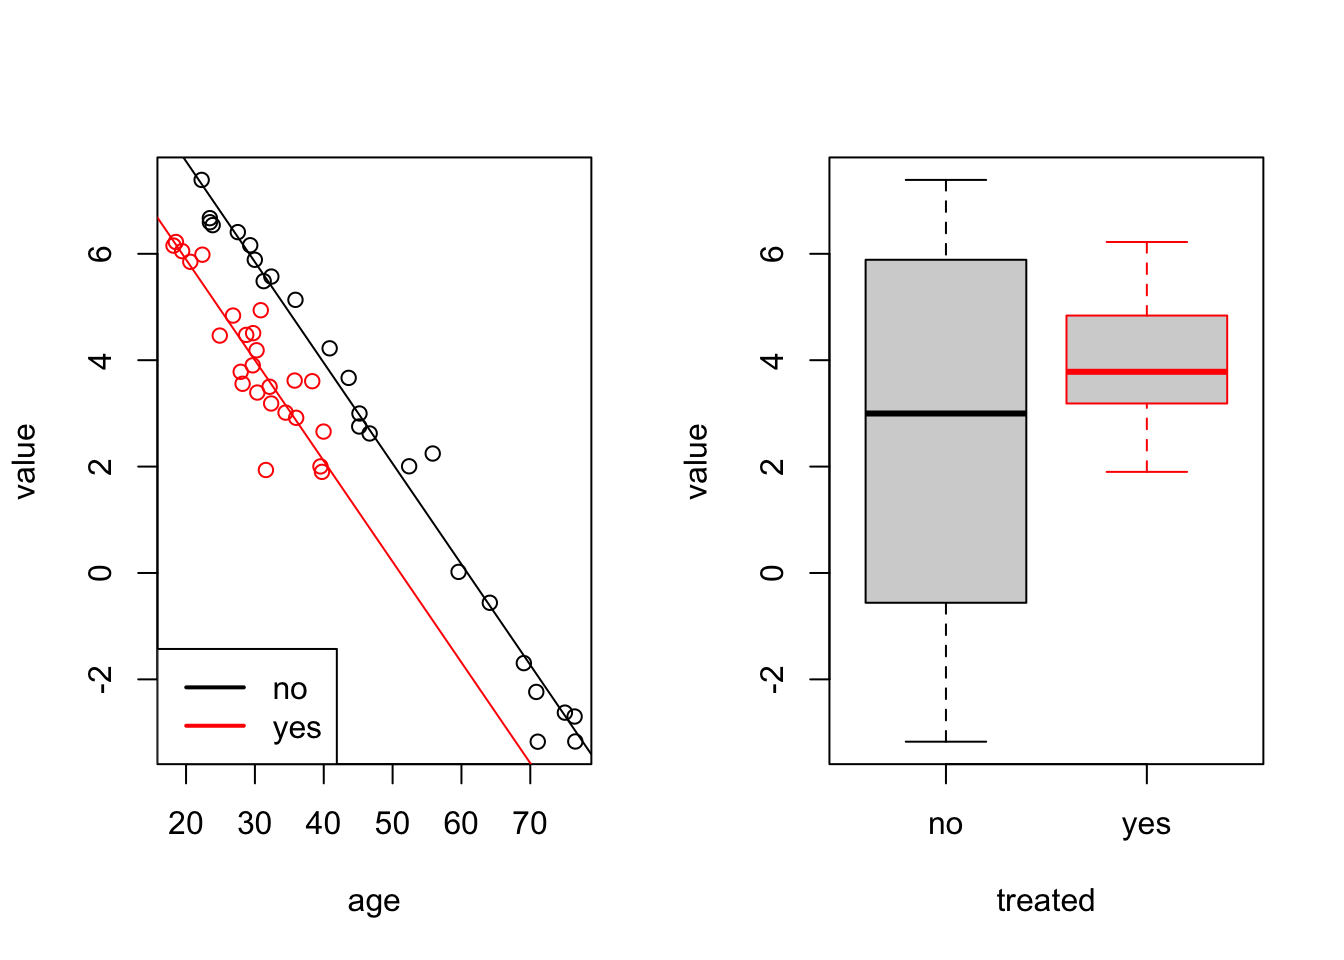
\includegraphics{MATH3714_files/figure-latex/factors-1.pdf}

We can see that the two regression lines, corresponding to the two levels
are parallel. They have the same slope but different intercepts.

The last command shows a boxplot of \texttt{value} for comparison.
The boxplot does not allow to conclude that the treatment had an effect,
whereas the linear model, which accounts for age, shows the effect
of the treatment as a difference in intercepts. The \texttt{***}
in the \texttt{treatedyes} row of the \texttt{summary(m)} output shows that the
difference in intercepts is statistically significant.
\end{example}

\hypertarget{interactions}{%
\subsection{Interactions}\label{interactions}}

In some situations, the strength of the dependency of the response \(y\) to an
input \(x_1\) might depend on another input, say \(x_2\). The simplest such
situation would be, if the coefficient \(\beta_1\), corresponding on \(x_1\) is
itself proportional to \(x_2\), say \(\beta_1 = \gamma x_2\). In this case we have
\(y = \cdots + \beta_1 x_1 = \cdots + \gamma x_1 x_2\). Traditionally, inputs
added to a model which are the product of two or more of the original inputs
are called \textbf{interactions}. As a general rule, an interaction is only included
if the ``main effects'' are also included in the model, so in any variable
selection procedure, we would not drop \(x_1\) or \(x_2\) if \(x_1 x_2\) is still in
the model. An exception to this is when one can directly interpret the
interaction term without the main effect.

In R, interactions (\emph{i.e.}~products of inputs) are represented by the
symbol~\texttt{:} and \texttt{*} can be used to include two variables together with their
product. Note also, that if a variable is known to be a factor, and it is
included as an interaction term, then R will make sure to only remove the
interaction term in a backward variable selection procedure whilst the main
effects are also included.

\begin{example}

Consider the following toy dataset:

\begin{Shaded}
\begin{Highlighting}[]
\NormalTok{x1 }\OtherTok{\textless{}{-}} \FunctionTok{c}\NormalTok{(}\DecValTok{2}\NormalTok{,}\DecValTok{2}\NormalTok{,}\DecValTok{2}\NormalTok{)}
\NormalTok{x2 }\OtherTok{\textless{}{-}} \DecValTok{1}\SpecialCharTok{:}\DecValTok{3}
\end{Highlighting}
\end{Shaded}

In \texttt{lm()} and related functions we can write \texttt{x1:x2} as a shorthand
for \texttt{I(x1*x2)}:

\begin{Shaded}
\begin{Highlighting}[]
\FunctionTok{model.matrix}\NormalTok{(}\SpecialCharTok{\textasciitilde{}}\NormalTok{ x1 }\SpecialCharTok{+}\NormalTok{ x1}\SpecialCharTok{:}\NormalTok{x2)}
\end{Highlighting}
\end{Shaded}

\begin{Shaded}
\begin{Highlighting}[]
\NormalTok{\#   (Intercept) x1 x1:x2}
\NormalTok{\# 1           1  2     2}
\NormalTok{\# 2           1  2     4}
\NormalTok{\# 3           1  2     6}
\NormalTok{\# attr(,"assign")}
\NormalTok{\# [1] 0 1 2}
\end{Highlighting}
\end{Shaded}

We can write \texttt{x1*x2} as a shorthand for \texttt{x1\ +\ x2\ +\ x1:x2}:

\begin{Shaded}
\begin{Highlighting}[]
\FunctionTok{model.matrix}\NormalTok{(}\SpecialCharTok{\textasciitilde{}}\NormalTok{ x1}\SpecialCharTok{*}\NormalTok{x2)}
\end{Highlighting}
\end{Shaded}

\begin{Shaded}
\begin{Highlighting}[]
\NormalTok{\#   (Intercept) x1 x2 x1:x2}
\NormalTok{\# 1           1  2  1     2}
\NormalTok{\# 2           1  2  2     4}
\NormalTok{\# 3           1  2  3     6}
\NormalTok{\# attr(,"assign")}
\NormalTok{\# [1] 0 1 2 3}
\end{Highlighting}
\end{Shaded}

\end{example}

Interactions also work for factors. In this case, products with all of
the corresponding indicator variables are added to the model. while
the base effect of factor variables is to have different intercepts for
the different groups, using interactions with a factor allows to have
different slopes for the different groups.

\begin{example}
The classical example of an interaction is to consider how the
yield~\(y\) of a crop is related to temperature~\(x_1\) and rainfall~\(x_2\).
All these variables are continuous, but we might categorize rainfall as ``wet''
and ``dry''. Then a simplistic view could be that, for high rainfall, the yield
will be positively correlated with temperature, whereas for low rainfall the
correlation may be slightly negative, because in hot weather, plants need more
water, and if it is very hot and dry, the plants may even die.

We generate a toy dataset in R to represent such a situation:

\begin{Shaded}
\begin{Highlighting}[]
\NormalTok{T }\OtherTok{\textless{}{-}} \FunctionTok{runif}\NormalTok{(}\DecValTok{25}\NormalTok{, }\DecValTok{15}\NormalTok{, }\DecValTok{35}\NormalTok{)}
\NormalTok{wet }\OtherTok{\textless{}{-}} \FunctionTok{data.frame}\NormalTok{(}
    \AttributeTok{yield=}\DecValTok{40} \SpecialCharTok{+} \DecValTok{7}\SpecialCharTok{*}\NormalTok{T }\SpecialCharTok{+} \FunctionTok{rnorm}\NormalTok{(}\DecValTok{25}\NormalTok{, }\AttributeTok{sd =} \DecValTok{10}\NormalTok{),}
    \AttributeTok{temperature=}\NormalTok{T,}
    \AttributeTok{rainfall=}\StringTok{"high"}\NormalTok{)}
\NormalTok{T }\OtherTok{\textless{}{-}} \FunctionTok{runif}\NormalTok{(}\DecValTok{25}\NormalTok{, }\DecValTok{15}\NormalTok{, }\DecValTok{35}\NormalTok{)}
\NormalTok{dry }\OtherTok{\textless{}{-}} \FunctionTok{data.frame}\NormalTok{(}
    \AttributeTok{yield=}\DecValTok{120} \SpecialCharTok{{-}} \DecValTok{2}\SpecialCharTok{*}\NormalTok{T }\SpecialCharTok{+} \FunctionTok{rnorm}\NormalTok{(}\DecValTok{25}\NormalTok{, }\AttributeTok{sd =} \DecValTok{10}\NormalTok{),}
    \AttributeTok{temperature=}\NormalTok{T,}
    \AttributeTok{rainfall=}\StringTok{"low"}\NormalTok{)}
\NormalTok{crops }\OtherTok{\textless{}{-}} \FunctionTok{rbind}\NormalTok{(wet, dry)}
\NormalTok{crops}\SpecialCharTok{$}\NormalTok{rainfall }\OtherTok{\textless{}{-}} \FunctionTok{factor}\NormalTok{(crops}\SpecialCharTok{$}\NormalTok{rainfall, }\AttributeTok{levels =} \FunctionTok{c}\NormalTok{(}\StringTok{"low"}\NormalTok{, }\StringTok{"high"}\NormalTok{))}
\end{Highlighting}
\end{Shaded}

Now we fit a model, including \texttt{temperature}, \texttt{rainfall} and
an interaction term:

\begin{Shaded}
\begin{Highlighting}[]
\NormalTok{m }\OtherTok{\textless{}{-}} \FunctionTok{lm}\NormalTok{(yield }\SpecialCharTok{\textasciitilde{}}\NormalTok{ temperature}\SpecialCharTok{*}\NormalTok{rainfall, }\AttributeTok{data =}\NormalTok{ crops)}
\FunctionTok{summary}\NormalTok{(m)}
\end{Highlighting}
\end{Shaded}

\begin{Shaded}
\begin{Highlighting}[]
\NormalTok{\# }
\NormalTok{\# Call:}
\NormalTok{\# lm(formula = yield \textasciitilde{} temperature * rainfall, data = crops)}
\NormalTok{\# }
\NormalTok{\# Residuals:}
\NormalTok{\#      Min       1Q   Median       3Q      Max }
\NormalTok{\# {-}22.8996  {-}6.3555   0.0346   5.9355  25.0553 }
\NormalTok{\# }
\NormalTok{\# Coefficients:}
\NormalTok{\#                          Estimate Std. Error t value Pr(\textgreater{}|t|)    }
\NormalTok{\# (Intercept)              114.2722     9.0929  12.567  \textless{} 2e{-}16 ***}
\NormalTok{\# temperature               {-}1.8873     0.3617  {-}5.219 4.21e{-}06 ***}
\NormalTok{\# rainfallhigh             {-}71.5892    13.0342  {-}5.492 1.66e{-}06 ***}
\NormalTok{\# temperature:rainfallhigh   8.7043     0.5299  16.428  \textless{} 2e{-}16 ***}
\NormalTok{\# {-}{-}{-}}
\NormalTok{\# Signif. codes:  0 \textquotesingle{}***\textquotesingle{} 0.001 \textquotesingle{}**\textquotesingle{} 0.01 \textquotesingle{}*\textquotesingle{} 0.05 \textquotesingle{}.\textquotesingle{} 0.1 \textquotesingle{} \textquotesingle{} 1}
\NormalTok{\# }
\NormalTok{\# Residual standard error: 10.42 on 46 degrees of freedom}
\NormalTok{\# Multiple R{-}squared:  0.9814,  Adjusted R{-}squared:  0.9802 }
\NormalTok{\# F{-}statistic: 810.2 on 3 and 46 DF,  p{-}value: \textless{} 2.2e{-}16}
\end{Highlighting}
\end{Shaded}

The fitted values for this model are
\begin{equation*}
  \hat y
  = \begin{cases}
    \beta_0 + \beta_1 x_1 & \mbox{for low rainfall, and} \\
    (\beta_0 + \beta_2) + (\beta_1 + \beta_3) x_1 & \mbox{for high rainfall}.
  \end{cases}
\end{equation*}
Finally, we can generate a plot of the data together
with the two regression lines.

\begin{Shaded}
\begin{Highlighting}[]
\FunctionTok{plot}\NormalTok{(yield }\SpecialCharTok{\textasciitilde{}}\NormalTok{ temperature, }\AttributeTok{data=}\NormalTok{crops,}
     \AttributeTok{col =} \FunctionTok{ifelse}\NormalTok{(rainfall }\SpecialCharTok{==} \StringTok{"low"}\NormalTok{, }\StringTok{"black"}\NormalTok{, }\StringTok{"red"}\NormalTok{))}
\FunctionTok{abline}\NormalTok{(}\AttributeTok{a =} \FunctionTok{coef}\NormalTok{(m)[}\DecValTok{1}\NormalTok{], }\AttributeTok{b =} \FunctionTok{coef}\NormalTok{(m)[}\DecValTok{2}\NormalTok{])}
\FunctionTok{abline}\NormalTok{(}\AttributeTok{a =} \FunctionTok{coef}\NormalTok{(m)[}\DecValTok{1}\NormalTok{] }\SpecialCharTok{+} \FunctionTok{coef}\NormalTok{(m)[}\DecValTok{3}\NormalTok{], }\AttributeTok{b =} \FunctionTok{coef}\NormalTok{(m)[}\DecValTok{2}\NormalTok{] }\SpecialCharTok{+} \FunctionTok{coef}\NormalTok{(m)[}\DecValTok{4}\NormalTok{],}
       \AttributeTok{col=}\StringTok{"red"}\NormalTok{)}
\FunctionTok{legend}\NormalTok{(}\StringTok{"topleft"}\NormalTok{, }\FunctionTok{c}\NormalTok{(}\StringTok{"dry"}\NormalTok{, }\StringTok{"wet"}\NormalTok{),}
       \AttributeTok{col =} \FunctionTok{c}\NormalTok{(}\StringTok{"black"}\NormalTok{, }\StringTok{"red"}\NormalTok{), }\AttributeTok{pch =} \DecValTok{1}\NormalTok{)}
\end{Highlighting}
\end{Shaded}

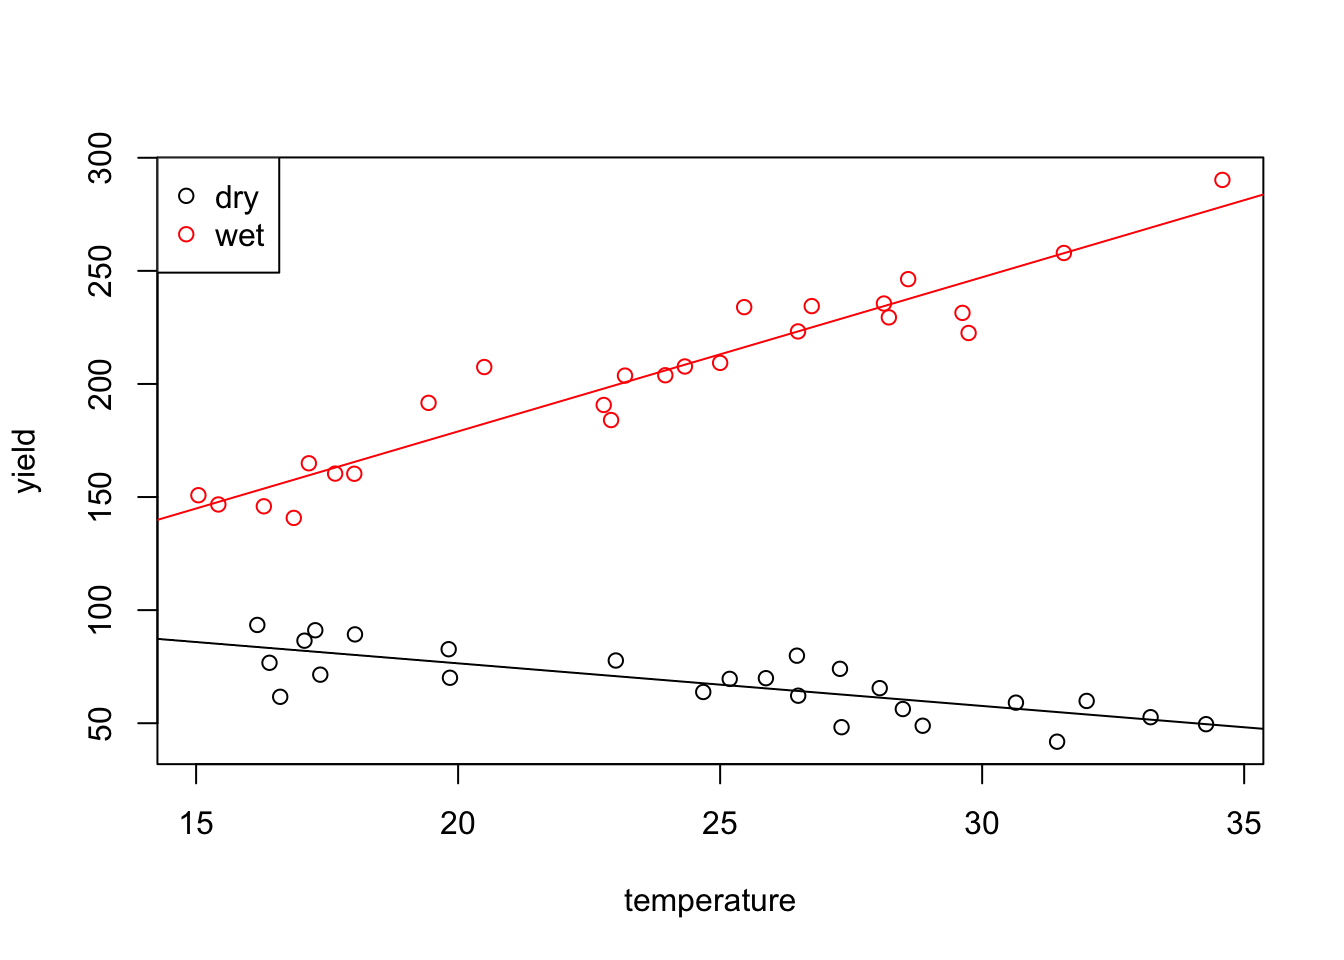
\includegraphics{MATH3714_files/figure-latex/interactions-1.pdf}

As expected, the two lines have different intercepts and different slopes.
\end{example}

\textbf{Summary}

\begin{itemize}
\tightlist
\item
  Indicator variables can be used to represent categorical inputs
  in linear regression models.
\item
  The levels of a factor correspond to different intercepts for
  the regression line.
\item
  If interaction terms are used, the levels also affect the slope.
\end{itemize}

\clearpage

\hypertarget{practical}{%
\section*{Practical}\label{practical}}
\addcontentsline{toc}{section}{Practical}

\begin{itemize}
\tightlist
\item
  The MATH3714 and MATH5714M modules are assessed by an examination (80\%)
  and a practical (20\%). This is the practical, worth 20\% of your final
  module mark.
\item
  You must hand in your solution
  by \textbf{Thursday, 9th December 2021, 5pm}, via Gradescope.
\item
  Reports must be typeset (not handwritten) and should be no more than 10 pages in length
  (but can be shorter).
\item
  Within reason you may talk to your friends about this piece of work,
  but you should not send R code (or output) to each other.
  Your report must be only your own work.
\end{itemize}

\hypertarget{dataset}{%
\subsection*{Dataset}\label{dataset}}
\addcontentsline{toc}{subsection}{Dataset}

In this practical we are interesting in factors which influence
the life expectancy at birth. We consider the following dataset:

\begin{itemize}
\tightlist
\item
  \url{https://www1.maths.leeds.ac.uk/~voss/2021/MATH3714/practical.csv}
\end{itemize}

You can read the data into R using the following command:

\begin{Shaded}
\begin{Highlighting}[]
\NormalTok{d }\OtherTok{\textless{}{-}} \FunctionTok{read.csv}\NormalTok{(}\StringTok{"https://www1.maths.leeds.ac.uk/\textasciitilde{}voss/2021/MATH3714/practical.csv"}\NormalTok{,}
              \AttributeTok{stringsAsFactors =} \ConstantTok{TRUE}\NormalTok{)}
\end{Highlighting}
\end{Shaded}

The dataset contain the following variables:

\begin{itemize}
\tightlist
\item
  \texttt{country}: country
\item
  \texttt{region}: geographic region the country is in
\item
  \texttt{sub.region}: geographic sub-region the country is in
\item
  \texttt{year}: year the data refers to
\item
  \texttt{gdp.per.capita}: Per capita GDP at current prices (USD)
\item
  \texttt{health.spending}: Per capita government expenditure on health at average exchange rate (USD,
  only until 2010)
\item
  \texttt{hiv}: Prevalence of HIV among adults aged 15 to 49 (\%)
\item
  \texttt{alcohol}: Alcohol, recorded per capita (15+) consumption (in litres of pure alcohol)
\item
  \texttt{tobacco}: Prevalence of current tobacco use among adults aged \(\geq 15\) years
\item
  \texttt{pop.size}: population size, for the given country and year (thousands)
\item
  \texttt{pop.density}: Population per square kilometre, for the given country and year (thousands)
\item
  \texttt{life.expectancy}: Life expectancy at birth (years). This is the variable we are interested in.
\end{itemize}

\hypertarget{tasks}{%
\subsection*{Tasks}\label{tasks}}
\addcontentsline{toc}{subsection}{Tasks}

The aim of this practical is to fit an appropriate model to these data, which
predicts the life expectancy \texttt{life.expectancy} from the other variables.

This practical is deliberately open-ended, with little guidance on how to proceed.

\textbf{Task 1.} We start by considering \texttt{life.expectancy} as a function
of \texttt{gdp.per.capita} only.

\begin{itemize}
\item
  Using appropriate transformations of the data, find a linear model which can
  describe the relationship between \texttt{life.expectancy} (response) and
  \texttt{gdp.per.capita} (input).
\item
  Using appropriate diagnostics, confirm that your model is acceptable.
  In your answer, you only need to describe your final model, and \emph{one} other
  model which you have examined, but deemed less appropriate.
\item
  Using your model obtain a 95\% confidence interval for the mean (expected)
  life expectancy at birth, for a country with a per capita GDP of 4000~USD.
\end{itemize}

\textbf{Task 2.} Now we also consider the remaining variables in the dataset.

\begin{itemize}
\item
  With due consideration to

  \begin{itemize}
  \tightlist
  \item
    transformations (where, and if, necessary)
  \item
    appropriate choice of variables
  \item
    model selection
  \item
    model checking
  \item
    variable selection
  \item
    missing data
  \item
    \emph{etc.}
  \end{itemize}

  obtain a model which is able to predict \texttt{life.expectancy} from some or all
  of the other variables.
\item
  Justify your choice by comparing at least two ``competing'' models.
  The comparison should take note of at
  least (a) model selection criteria, (b) diagnostics, and (c) interpretability.
\item
  Interpret the parameters in your preferred model.
\end{itemize}

There is no single right or wrong answer to this practical.
The important thing is that you justify your approach.

\hypertarget{references}{%
\subsection*{References}\label{references}}
\addcontentsline{toc}{subsection}{References}

The data were collected from the following sources.

\begin{itemize}
\tightlist
\item
  \url{https://www.who.int/data/gho/data/indicators/indicator-details/GHO/life-expectancy-at-birth-(years)}
  \texttt{country}, \texttt{year}, \texttt{lift.expectancy}
\item
  \url{https://population.un.org/wpp/Download/Standard/CSV/}
  \texttt{country}, \texttt{year}, \texttt{pop.size}, \texttt{pop.density}, \texttt{region}, \texttt{sub.region}
\item
  \url{https://data.un.org/Data.aspx?d=SNAAMA\&f=grID\%3A101\%3BcurrID\%3AUSD\%3BpcFlag\%3A1}
  \texttt{country}, \texttt{year}, \texttt{gdp.per.capita}
\item
  \url{http://data.un.org/Data.aspx?d=WHO\&f=MEASURE_CODE\%3aWHS7_104}
  \texttt{country}, \texttt{year}, \texttt{health.spending}
\item
  \url{https://www.who.int/data/gho/data/indicators/indicator-details/GHO/alcohol-recorded-per-capita-(15-)-consumption-(in-litres-of-pure-alcohol)}
  \texttt{country}, \texttt{year}, \texttt{alcohol}
\item
  \url{https://www.who.int/data/gho/data/indicators/indicator-details/GHO/age-standardized-prevalence-of-current-tobacco-smoking-among-persons-aged-15-years-and-older}
  \texttt{country}, \texttt{year}, \texttt{tobacco}
\item
  \url{https://www.who.int/data/gho/data/indicators/indicator-details/GHO/prevalence-of-hiv-among-adults-aged-15-to-49-(-)}
  \texttt{country}, \texttt{year}, \texttt{hiv}
\end{itemize}

\clearpage

\hypertarget{appendix-appendices}{%
\appendix}


\hypertarget{Sx1-matrices}{%
\section{Linear Algebra Reminders}\label{Sx1-matrices}}

\hypertarget{vectors}{%
\subsection{Vectors}\label{vectors}}

We write \(v \in \mathbb{R}^d\) if \(v = (v_1, \ldots, v_d)\) for numbers
\(v_1, \ldots, v_d \in\mathbb{R}\). We say that \(v\) is a \(d\)-dimensional vector,
and \(\mathbb{R}^d\) is the \(d\)-dimensional Euclidean space. Vectors are
often graphically represented as ``column vectors'':
\begin{equation*}
  v = \begin{pmatrix}
      v_1 \\ v_2 \\ \vdots \\ v_d
  \end{pmatrix}.
\end{equation*}

If \(u,v\in\mathbb{R}^d\) are two vectors, the \textbf{inner product} of \(u\) and~\(v\)
is given by
\begin{equation}
  u^\top v
  = \sum_{i=1}^d u_i v_i.  \label{eq:inner-product}
\end{equation}
Note that the two vectors must have the same length for the inner product
to exist.

Using this notation, the \textbf{Euclidean length} of a vector~\(v\)
can be written as
\begin{equation*}
  \|v\|
  = \sqrt{\sum_{i=1}^d v_i^2}
  = \sqrt{v^\top v}.
\end{equation*}

Vectors \(v_1, \ldots, v_n\) are said to be \textbf{orthogonal},
if \(v_i^\top v_j = 0\) for all \(i \neq j\). The vectors are said to be
\textbf{orthonormal}, if they are orthogonal and satisfy \(\|v_i\| = 1\)
for all~\(i\).

\hypertarget{matrix-rules}{%
\subsection{Matrices}\label{matrix-rules}}

We write \(A \in \mathbb{R}^{m\times n}\) if
\begin{equation*}
  A
  = \begin{pmatrix}
    a_{1,1} & \ldots  & a_{1,n}\\
    a_{2,1} & \ldots  & a_{2,n}\\
    \vdots & \ddots  & \vdots\\
    a_{m,1} & \ldots  & a_{m,n}
  \end{pmatrix},
\end{equation*}
where \(a_{i,j}\), sometimes also written as \(a_{ij}\) are numbers
for \(i \in \{1, \ldots, m\}\) and \(j \in \{1, \ldots, n\}\).

\hypertarget{transpose}{%
\subsubsection{Transpose}\label{transpose}}

If \(A \in \mathbb{R}^{m\times n}\), then the \textbf{transpose} of \(A\) is the matrix
\(A^\top \in \mathbb{R}^{n\times m}\), with \((A^\top)_{ij} = a_{ji}\) for all \(i \in \{1, \ldots, n\}\) and \(j \in \{1, \ldots, m\}\). Graphically,
this can be written as
\begin{equation*}
  A^\top
  = \begin{pmatrix}
    a_{1,1} & a_{2,1} \ldots  & a_{m,1}\\
    \vdots & \vdots & \ddots  & \vdots\\
    a_{1,n} & a_{2,n} \ldots  & a_{m,n}
  \end{pmatrix},
\end{equation*}

\begin{definition}
A matrix \(A\) is called \textbf{symmetric}, if \(A^\top = A\).
\end{definition}

\hypertarget{matrix-vector-product}{%
\subsubsection{Matrix-vector Product}\label{matrix-vector-product}}

If \(A \in \mathbb{R}^{m \times n}\) and \(v \in \mathbb{R}^n\), then
\(Av \in \mathbb{R}^m\) is the vector with
\begin{equation*}
  (Av)_i
  = \sum_{j=1}^n a_{ij} v_j
\end{equation*}
for all \(i \in \{1, \ldots, m\}\).

If we consider \(v\) to be a \((n\times 1)\)-matrix instead of a vector,
\(Av\) can also be interpreted as a matrix-matrix product between an \(m \times n\) and an \(n\times 1\) matrix. Using this convention, \(v^\top\)
is then interpreted as an \(1 \times n\) matrix and if \(u\in\mathbb{R}^m\) we
have \(u^\top A \in \mathbb{R}^{1 \times n} \cong \mathbb{R}^n\) with
\begin{equation*}
  (u^\top A)_j
  = \sum_{i=1}^m u_i a_{ij}
\end{equation*}
for all \(j \in \{1, \ldots, n\}\). Going one step further, this
notation also motivates the expression \(u^\top v\) in
equation~\eqref{eq:inner-product}.

\hypertarget{matrix-matrix-product}{%
\subsubsection{Matrix-matrix Product}\label{matrix-matrix-product}}

If \(A \in \mathbb{R}^{\ell \times m}\) and \(B \in \mathbb{R}^{m\times n}\), then
\(AB \in \mathbb{R}^{\ell \times n}\) is the matrix with
\begin{equation*}
  (AB)_{ik}
  = \sum_{j=1}^m a_{ij} b_{jk}
\end{equation*}
for all \(i \in \{1, \ldots, \ell\}\) and \(j \in \{1, \ldots, n\}\).
This is called the \textbf{matrix product} of \(A\) and \(B\). Note
that \(A\) and \(B\) must have compatible shapes for the product to exist.

Properties:

\begin{itemize}
\item
  The matrix product is associative: if \(A\), \(B\) and \(C\) are matrices
  with shapes such that \(AB\) and \(BC\) exist, then we have \(A(BC) = (AB)C\).
  It does not matter in which order we perform the matrix products here.
\item
  The matrix product is transitive: if \(A\), \(B\) and \(C\) have the
  correct shapes, we have \(A(B+C) = AB + AC\).
\item
  The matrix product is \emph{not} commutative: if \(AB\) exists, in general
  \(A\) and \(B\) don't have the correct shapes for \(BA\) to also exist,
  and even if \(BA\) exists, in general we have \(AB \neq BA\).
\item
  Taking the transpose swaps the order in a matrix product:
  we have
  \begin{equation}
    (AB)^\top = B^\top A^\top  \label{eq:AB-trans}
  \end{equation}
\end{itemize}

\hypertarget{rank}{%
\subsubsection{Rank}\label{rank}}

\begin{definition}
The \textbf{rank} of a matrix~\(A \in \mathbb{R}^{m \times n}\) is the dimension of the
image space of~\(A\):
\begin{equation*}
  \mathop{\mathrm{rank}}(A)
  = \dim \bigl\{ Av \bigm| v\in \mathbb{R}^n \}.
\end{equation*}
\end{definition}

The rank can also be characterised as the largest number of linearly
independent columns of \(A\), or the largest number of linearly
independent rows of \(A\). Thus, for \(A \in \mathbb{R}^{m \times n}\) we
always have \(\mathop{\mathrm{rank}}(A) \leq \min(m, n)\). The matrix \(A\)
is said to have ``full rank'' if \(\mathop{\mathrm{rank}}(A) = \min(m, n)\).

\hypertarget{trace}{%
\subsubsection{Trace}\label{trace}}

\begin{definition}
The \textbf{trace} of a matrix \(A \in \mathbb{R}^{n\times n}\) is given by
\begin{equation*}
  \mathop{\mathrm{tr}}(A) = \sum_{i=1}^n a_ii.
\end{equation*}
\end{definition}

Properties:

\begin{itemize}
\item
  \(\mathop{\mathrm{tr}}(A+B) = \mathop{\mathrm{tr}}(A) + \mathop{\mathrm{tr}}(B)\)
\item
  \(\mathop{\mathrm{tr}}(A^\top) = \mathop{\mathrm{tr}}(A)\)
\item
  \(\mathop{\mathrm{tr}}(ABC) = \mathop{\mathrm{tr}}(BCA) = \mathop{\mathrm{tr}}(CAB)\). The individual matrices \(A, B, C\) don't
  need to be square for this relation to hold, but the relation only holds for
  cyclic permutations as shown. In general \(\mathop{\mathrm{tr}}(ABC) \neq \mathop{\mathrm{tr}}(ACB)\).
\end{itemize}

\hypertarget{matrix-inverse}{%
\subsubsection{Matrix Inverse}\label{matrix-inverse}}

If \(A\) is a square matrix and if there is a matrix \(B\) such that
\(AB = I\), then \(A\) is called \textbf{invertible} and the matrix \(B\) is
called the \textbf{inverse} of~\(A\), denoted by \(A^{-1} := B\).
Some important properties of the inverse:

\begin{itemize}
\item
  The inverse, if it exists, is unique.
\item
  Left-inverse and right-inverse for matrices are the same:
  \(A^{-1} A = I\) holds if and only if \(A A^{-1} = I\).
\item
  If \(A\) is symmetric and invertible, then \(A^{-1}\) is also
  symmetric. This is true because \(A (A^{-1})^\top = (A^{-1} A)^\top = I^\top = I\) and thus \((A^{-1})^\top\) is an inverse of \(A\).
  Since the inverse is unique, \((A^{-1})^\top = A^{-1}\).
\end{itemize}

\begin{theorem}
\protect\hypertarget{thm:matrix-inverse}{}\label{thm:matrix-inverse}

Let \(A \in \mathbb{R}^{n\times n}\). Then the following statements are equivalent:

\begin{enumerate}
\def\labelenumi{\alph{enumi}.}
\tightlist
\item
  \(A\) is invertible
\item
  \(A\) has full rank, \emph{i.e.} \(\mathop{\mathrm{rank}}(A) = n\).
\item
  The equation \(Ax = 0\) has \(x = 0\) as its only solution.
\item
  The equation \(Ax = b\) has exactly one solution \(x\) for every
  \(b\in\mathbb{R}^n\).
\end{enumerate}

\end{theorem}

\hypertarget{orthogonal-matrices}{%
\subsubsection{Orthogonal Matrices}\label{orthogonal-matrices}}

\begin{definition}
A matrix \(U\) is called \textbf{orthogonal}, if \(U^\top U = I = U U^\top\).
\end{definition}

Some important properties of orthogonal matrices:

\begin{itemize}
\item
  If \(U\) is orthogonal, the inverse and the transpose are the same:
  \(U^\top = U^{-1}\).
\item
  We have \(\| U x \|^2 = x^\top U^\top U x = x^\top x = \| x \|^2\).
  Thus, multiplying a vector \(x\) by an orthogonal matrix \(U\) does
  not change its length.
\end{itemize}

\hypertarget{positive-definite}{%
\subsubsection{Positive Definite Matrices}\label{positive-definite}}

\begin{definition}
A symmetric matrix \(A \in \mathbb{R}^{n\times n}\) is called \textbf{positive definite}, if
\begin{equation*}
  x^\top A x > 0
\end{equation*}
for all \(x \in \mathbb{R}^n\) with \(x\neq 0\). The matrix is called
\textbf{positive semi-definite}, if
\begin{equation*}
  x^\top A x \geq 0
\end{equation*}
for all \(x \in \mathbb{R}^n\).
\end{definition}

\hypertarget{idempotent}{%
\subsubsection{Idempotent Matrices}\label{idempotent}}

\begin{definition}
The matrix \(A\) is \textbf{idempotent}, if \(A^2 = A\).
\end{definition}

\hypertarget{eigenvalues}{%
\subsection{Eigenvalues}\label{eigenvalues}}

\begin{definition}
Let \(A \in\mathbb{R}^{n\times n}\) be a square matrix and \(\lambda\in R\).
The number \(\lambda\) is called an \textbf{eigenvalue} of \(A\), if there
exists a vector \(v \neq 0\) such that \(A x = \lambda x\). Any
such vector \(x\) is called an \textbf{eigenvector} of \(A\) with eigenvalue~\(\lambda\).
\end{definition}

While there are very many results about eigenvectors and eigenvalues
in Linear Algebra, here we will only use a small number of these results.
We summarise what we need for this module:

\begin{itemize}
\tightlist
\item
  If \(A\) is idempotent and \(x\) is an eigenvector with eigenvalue \(\lambda\),
  then we have \(\lambda x = A x = A^2 x = \lambda Ax = \lambda^2 x\). Thus we
  have \(\lambda^2 = \lambda\). This shows that the only eigenvalues possible
  for idempotent matrices are \(0\) and~\(1\).
\end{itemize}

\begin{theorem}
\protect\hypertarget{thm:spectral}{}\label{thm:spectral}Let \(A\in\mathbb{R}^{n\times n}\) be symmetric. Then there is an orthogonal
matrix \(U\) such that \(D := U A U^\top\) is diagonal. The diagonal
elements of \(D\) are the eigenvalues of \(A\) and the rows of \(U\)
are corresponding eigenvectors.
\end{theorem}

\clearpage

\hypertarget{Sx2-probability}{%
\section{Probability Reminders}\label{Sx2-probability}}

\hypertarget{independence}{%
\subsection{Independence}\label{independence}}

\begin{definition}
Two random variables \(X\) and \(Y\) are (statistically) \textbf{independent}, if
\(P(X\in A, Y\in B) = P(X\in A) P(Y\in B)\) for all sets \(A\) and~\(B\).
\end{definition}

We list some properties of independent random variables:

\begin{itemize}
\tightlist
\item
  If \(X\) and \(Y\) are independent, and if \(f\) and \(g\) are functions,
  then \(f(X)\) and \(g(Y)\) are also independent.
\end{itemize}

\hypertarget{chi-square}{%
\subsection{The Chi-Squared Distribution}\label{chi-square}}

\begin{definition}
\protect\hypertarget{def:chi-squared-dist}{}\label{def:chi-squared-dist}Let \(X_1, \ldots, X_\nu \sim \mathcal{N}(0, 1)\) be i.i.d. Then the
distribution of \(\sum_{i=1}^\nu X_i^2\) is called the
\(\chi^2\)-distribution with \(\nu\) degrees of freedom. The
distribution is denoted by~\(\chi^2(\nu)\).
\end{definition}

Some important results about the \(\chi^2\)-distribution are:

\begin{itemize}
\item
  \(\chi^2\)-distributed random variables are always positive.
\item
  If \(Y\sim \chi^2(\nu)\), then \(\mathbb{E}(Y) = \nu\) and \(\mathop{\mathrm{Var}}(Y) = 2\nu\).
\item
  The R command \texttt{pchisq(\textbar{}}\(x\)\texttt{,}\(\nu\)\texttt{)} gives the value
  \(\Phi_\nu(x)\) of the CDF of the \(\chi^2(\nu)\)-distribution.
\item
  The R command \texttt{qchisq(}\(\alpha\)\texttt{,}\(\nu\)\texttt{)} can
  be used to obtain the
  \(\alpha\)-quantile of the \(\chi^2(\nu)\)-distribution.
\item
  More properties can be found
  \href{https://en.wikipedia.org/wiki/Chi-squared_distribution}{on Wikipedia}.
\end{itemize}

\hypertarget{t}{%
\subsection{The t-distribution}\label{t}}

\begin{definition}
\protect\hypertarget{def:t-dist}{}\label{def:t-dist}Let \(Z \sim \mathcal{N}(0,1)\) and \(Y \sim \chi^2(\nu)\) be independent. Then
the distribution of
\begin{equation}
  T
  = \frac{\,Z\,}{\,\sqrt{Y / \nu}\,}  \label{eq:t-def}
\end{equation}
is called the \(t\)-distribution with \(\nu\) degrees of freedom.
This distribution is denoted by~\(t(\nu)\).
\end{definition}

Some important results about the \(t\)-distribution are:

\begin{itemize}
\item
  The \(t\)-distribution is symmetric: if \(T \sim t(\nu)\), then
  \(-T \sim t(\nu)\)
\item
  If \(T\sim t(\nu)\), then \(\mathbb{E}(T) = 0\).
\item
  The R command \texttt{pt(\textbar{}}\(x\)\texttt{,}\(\nu\)\texttt{)} gives the value
  \(\Phi_\nu(x)\) of the CDF of the \(t(\nu)\)-distribution.
\item
  The R command \texttt{qt(}\(\alpha\)\texttt{,}\(\nu\)\texttt{)} can
  be used to obtain the
  \(\alpha\)-quantile of the \(t(\nu)\)-distribution.
\item
  More properties can be found
  \href{https://en.wikipedia.org/wiki/Student\%27s_t-distribution}{on Wikipedia}.
\end{itemize}

\clearpage

\end{document}
